% ******************************* PhD Thesis Template **************************

% Print version
%\documentclass[a4paper,11pt,times,custombib,print,index,custommargin]{Classes/PhDThesisPSnPDF}

% Online version
%\documentclass[a4paper,11pt,times,custombib,custommargin]{Classes/PhDThesisPSnPDF}
\documentclass[a4paper,11pt,times,custombib,custommargin,draftclassic]{Classes/PhDThesisPSnPDF}



% ******************************************************************************
% ******************************* Class Options ********************************
% ******************************************************************************

% `a4paper'(The University of Cambridge PhD thesis guidelines recommends a page size a4 - default option)
%
% `11pt' (default) or `12pt': Font Size 10pt is NOT recommended by the University guidelines
%
% `oneside' or `twoside'(default): Printing double side or single side.
%
% `print': Use `print' for print version with appropriate margins and page
% layout. Leaving the options field blank will activate Online version.
%
% `index': For index at the end of the thesis
%
% `draftclassic': For draft mode without loading any images (same as draft in book)
%
% `draft': Special draft mode with line numbers, images, and water mark with
% timestamp and custom text. Position of the text can also be modified.
%
% `abstract': To generate only the title page and abstract page with
% dissertation title and name, to submit to the Student Registry
%
% `chapter`: This option enables only the specified chapter and it's references
%  Useful for review and corrections.
%
% ************************* Custom Page Margins ********************************
%
% `custommargin`: Use `custommargin' in options to activate custom page margins,
% which can be defined in the preamble.tex. Custom margin will override
% print/online margin setup.
%
% *********************** Choosing the Fonts in Class Options ******************
%
% `times' : Times font with math support. (in Cambridge University guidelines)
%
% `fourier': Utopia Font with Fourier Math font (Font has to be installed)
%            It's a free font.
%
% `customfont': Use `customfont' option in the document class and load the
% package in the preamble.tex
%
% default or leave empty: `Latin Modern' font will be loaded.
%
% ********************** Choosing the Bibliography style ***********************
%
% `authoryear': For author-year citation eg., Krishna (2013)
%
% `numbered': (Default Option) For numbered and sorted citation e.g., [1,5,2]
%
% `custombib': Define your own bibliography style in the `preamble.tex' file.
%              `\RequirePackage[square, sort, numbers, authoryear]{natbib}'.
%              This can be also used to load biblatex instead of natbib
%              (See Preamble)
%
% **************************** Choosing the Page Style *************************
%
% `default (leave empty)': For Page Numbers in Header (Left Even, Right Odd) and
% Chapter Name in Header (Right Even) and Section Name (Left Odd). Blank Footer.
%
% `PageStyleI': Chapter Name next & Page Number on Even Side (Left Even).
% Section Name & Page Number in Header on Odd Side (Right Odd). Footer is empty.
%
% `PageStyleII': Chapter Name on Even Side (Left Even) in Header. Section Number
% and Section Name in Header on Odd Side (Right Odd). Page numbering in footer

% Uncomment to change page style
%\pagestyle{PageStyleII}

% ********************************** Preamble **********************************

% Contains packages and user-defined commands and settings
% ****************************** Custom Margin *********************************

% Add `custommargin' in the document class options to use this section
% Set {innerside margin / outerside margin / topmargin / bottom margin}  and
% other page dimensions
\ifsetCustomMargin
  \RequirePackage[left=23mm,right=23mm,top=27mm,bottom=22mm]{geometry}
%  \RequirePackage[left=37mm,right=30mm,top=35mm,bottom=30mm]{geometry}
  %\setFancyHdr % To apply fancy header after geometry package is loaded
\fi

% Define paragraph settings
\setlength{\parskip}{0.7em}  % space between paragraphs
\setlength{\parindent}{0pt}  % indentation

% Ragged bottom avoids extra whitespaces between paragraphs
\raggedbottom

% To remove the excess top spacing for enumeration, list and description
%\usepackage{enumitem}
%\setlist[enumerate,itemize,description]{topsep=0em}

% To remove the excess top spacing for titles
\usepackage{titlesec}
\titleformat{\chapter}[display]{\normalfont\huge\bfseries}{\chaptertitlename\ \thechapter}{20pt}{\Huge}   
\titleformat*{\section}{\LARGE\bfseries}
\titleformat*{\subsection}{\Large\bfseries}
\titleformat*{\subsubsection}{\large\bfseries}
\titleformat*{\paragraph}{\large\bfseries}


\titlespacing*{\chapter}{0pt}{-30pt}{20pt}
% \titlespacing*{\section}{0pt}{0pt}{0pt}
% \titlespacing*{\subsection}{0pt}{0pt}{0pt}
% \titlespacing*{\subsubsection}{0pt}{0pt}{0pt}

% Don't change this
% \titlespacing*{\section}{0pt}{12pt plus 4pt minus 2pt}{0pt plus 2pt minus 2pt}
% \titlespacing*{\subsection}{0pt}{12pt plus 4pt minus 2pt}{0pt plus 2pt minus 2pt}
% \titlespacing*{\subsubsection}{0pt}{12pt plus 4pt minus 2pt}{0pt plus 2pt minus 2pt}

% ************************* Algorithms and Pseudocode **************************
\usepackage{algorithm}
%\usepackage{algpseudocode}
%\usepackage[noend]{algpseudocode}


% ********************Captions and Hyperreferencing / URL **********************

% to support older versions of captions.sty
%\renewcommand{\figurename}{Fig.} 

% Captions for figures and subfigures
%\RequirePackage[small,bf]{caption} % This makes captions of figures use a boldfaced small font.
%\RequirePackage[labelsep=space,tableposition=top]{caption}
\RequirePackage[font={small}, margin=20pt, labelfont=bf]{caption}
\RequirePackage[font={footnotesize}, margin=20pt]{subcaption}


% Classic Draft Mode
\ifsetDraftClassic
\DeclareCaptionFormat{empty}{}
\captionsetup{format=empty}
%\captionsetup{format=empty,aboveskip=0pt,belowskip=0pt}
\fi


% *************************** Graphics and figures *****************************

%\usepackage{rotating}
%\usepackage{wrapfig}
\usepackage[section]{placeins}

% Uncomment the following two lines to force Latex to place the figure.
% Use [H] when including graphics. Note 'H' instead of 'h'
% \usepackage{float}
% \restylefloat{figure}

% Subcaption package is also available in the sty folder you can use that by
% uncommenting the following line
% This is for people stuck with older versions of texlive
%\usepackage{sty/caption/subcaption}
\usepackage{subcaption}

% ********************************** Tables ************************************
\usepackage{booktabs} % For professional looking tables
\usepackage{multirow}

\usepackage{multicol}
\usepackage{longtable}
\usepackage{tabularx}


% *********************************** SI Units *********************************

%\usepackage{siunitx}

% ******************************* Line Spacing *********************************

% Default is one-half line spacing as per the University guidelines

% \doublespacing
\onehalfspacing
% \singlespacing


% ************************ Formatting / Footnote *******************************

% Don't break enumeration (etc.) across pages in an ugly manner (default 10000)
%\clubpenalty=500
%\widowpenalty=500

%\usepackage[perpage]{footmisc} %Range of footnote options


% *************************** Graphical models ********************

\usepackage{tikz}
\usetikzlibrary{positioning}
\usetikzlibrary{bayesnet}

% *************************** Bibliography  and References ********************

% References
%\usepackage{hyperref}             % Hyperlink in references
\usepackage[nameinlink]{cleveref}  % Clever references (Cref)

% Per-chapter numbering of figures
\usepackage{chngcntr}
\counterwithin{figure}{chapter}


% Bibliography
% \RequirePackage[backend=biber, style=numeric-comp, citestyle=numeric, sorting=nty, natbib=true]{biblatex}
\RequirePackage[hyperref=true, url=false, backref=false, backend=biber, style=numeric,giveninits=true]{biblatex}

% Add bib resources
\addbibresource{references/references_chapter1.bib}
\addbibresource{references/references_chapter2.bib}
\addbibresource{references/references_chapter3.bib}
\addbibresource{references/references_chapter4.bib}
\addbibresource{references/references_chapter5.bib}

% changes the default name `Bibliography` -> `References'
% \renewcommand{\bibname}{References}

% ******************************************************************************
% ************************* User Defined Commands ******************************
% ******************************************************************************

% *********** To change the name of Table of Contents / LOF and LOT ************

%\renewcommand{\contentsname}{My Table of Contents}
%\renewcommand{\listfigurename}{My List of Figures}
%\renewcommand{\listtablename}{My List of Tables}

% ********************** TOC depth and numbering depth *************************

% Spacing in the TOC
\usepackage{tocloft}
\renewcommand\cftchapafterpnum{\vskip1pt}
\renewcommand\cftsecafterpnum{\vskip1pt}

% Depth in the TOC
% The sectioning levels have the following numbers:
% -1 part     1 section     3 subsubsection  5 subparagraph
%  0 chapter  2 subsection  4 paragraph

% The "tocdepth" value determines to which level the sectioning commands are printed in the ToC
\setcounter{tocdepth}{2}  % Default was 2

% The "secnumdepth" value determines up to what level the sectioning titles are numbered
\setcounter{secnumdepth}{2}  % Default was 2



% ******************************* Nomenclature *********************************

% To change the name of the Nomenclature section, uncomment the following line

%\renewcommand{\nomname}{Symbols}


% ********************************* Appendix ***********************************

% The default value of both \appendixtocname and \appendixpagename is `Appendices'. These names can all be changed via:

\renewcommand{\appendixtocname}{List of appendices}
\renewcommand{\appendixname}{Appendix}

% *********************** Configure Draft Mode **********************************

% Uncomment to disable figures in `draft'
%\setkeys{Gin}{draft=true}  % set draft to false to enable figures in `draft'

% These options are active only during the draft mode
% Default text is "Draft"
%\SetDraftText{DRAFT}

% Default Watermark location is top. Location (top/bottom)
%\SetDraftWMPosition{bottom}

% Draft Version - default is v1.0
%\SetDraftVersion{v1.1}

% Draft Text grayscale value (should be between 0-black and 1-white)
% Default value is 0.75
%\SetDraftGrayScale{0.8}


% ******************************** Todo Notes **********************************
%% Uncomment the following lines to have todonotes.

%\ifsetDraft
%	\usepackage[colorinlistoftodos]{todonotes}
%	\newcommand{\mynote}[1]{\todo[author=kks32,size=\small,inline,color=green!40]{#1}}
%\else
%	\newcommand{\mynote}[1]{}
%	\newcommand{\listoftodos}{}
%\fi

% Example todo: \mynote{Hey! I have a note}

% ******************* Better enumeration *************
\usepackage{enumitem}
 

% ************************ Thesis Information & Meta-data **********************

% ************************ Thesis Information & Meta-data **********************

%% The title of the thesis
\title{Statistical framework for the integration of single-cell multi-omics data sets}
%\texorpdfstring is used for PDF metadata. Usage:
%\texorpdfstring{LaTeX_Version}{PDF Version (non-latex)} eg.,
%\texorpdfstring{$sigma$}{sigma}

%% Subtitle (Optional)
% \subtitle{and applications to spatial expression data}

%% The full name of the author
\author{Ricard Argelaguet}

%% Department (eg. Department of Engineering, Maths, Physics)
\dept{European Bioinformatics Institute}

%% University and Crest
\university{University of Cambridge}
% Crest minimum should be 30mm.
\crest{
\includegraphics[width=0.2\textwidth]{University_Crest}}
%% Use this crest, if you are using the college crest
%% Crest long miminum should be 65mm
%\crest{
\includegraphics[width=0.45\textwidth]{University_Crest_Long}}

%% College shield [optional]
% Crest minimum should be 30mm.
%\collegeshield{\includegraphics[width=0.2\textwidth]{CollegeShields/Kings}}


%% Supervisor (optional)
%% for multiple supervisors, append each supervisor with the \newline command
%\supervisor{Prof. A.B. Supervisor\newline
%Prof. C.D. Supervisor}

%% Supervisor Role (optional) - Supervisor (default) or advisor
% \supervisorrole{\textbf{Supervisors: }}
%% if no title is desired:
% \supervisorrole{}

%% Supervisor line width: required to align supervisors
%\supervisorlinewidth{0.35\textwidth}

%% Advisor (optional)
%% for multiple advisors, append each advisor with the \newline command
%\advisor{Dr. A. Advisor\newline
%Dr. B. Advisor}

%% Advisor Role (optional) - Advisor (default) or leave empty
% \advisorrole{Advisors: }
%% if no title is required
% \advisorrole{}

%% Advisor line width: required to align supervisors
%\advisorlinewidth{0.25\textwidth}


%% You can redefine the submission text:
% Default as per the University guidelines:
% ``This dissertation is submitted for the degree of''
%\renewcommand{\submissiontext}{change the default text here if needed}

%% Full title of the Degree
\degreetitle{Doctor of Philosophy}

%% College affiliation (optional)
\college{Robinson College}

%% Submission date
% Default is set as {\monthname[\the\month]\space\the\year}
%\degreedate{September 2014}

%% Meta information
% \subject{LaTeX} \keywords{{LaTeX} {PhD Thesis} {Engineering} {University of
% Cambridge}}


%%%%% PERSONAL STUFF HERE %%%%%%%%%%%%

\usepackage{listings}

\usepackage{graphicx}
\usepackage{multicol}
\usepackage{stmaryrd}

% Math
\usepackage{dsfont} % Dirac Delta
\usepackage{amsmath}

% %TODO declare not as math operator to avoid weird upperscript
% \DeclareMathOperator*{\argmax}{\mathop{arg\,max}}
% \DeclareMathOperator*{\argmin}{\mathop{arg\,min}}
% \newcommand{\N}{\mathcal{N}}
% \newcommand{\dd}{\mathrm{d}}
% \newcommand{\KL}{\mathrm{KL}}
% \newcommand{\LL}{\mathcal{L}}
% \newcommand{\cov}{\mathrm{cov}}
% \DeclareMathOperator*{\E}{\mathop{\mathbb{E}}}
% \newcommand{\diff}{\mathrm{d}}
% \newcommand{\la}{\left\langle}
% \newcommand{\ra}{\right\rangle}
% \renewcommand{\labelenumi}{\roman{enumi}) }


\definecolor{codegreen}{rgb}{0,0.6,0}
\definecolor{codegray}{rgb}{0.5,0.5,0.5}
\definecolor{codepurple}{rgb}{0.58,0,0.82}
\definecolor{backcolour}{rgb}{0.95,0.95,0.92}

\lstdefinestyle{mystyle}{
    backgroundcolor=\color{backcolour},
    commentstyle=\color{codegreen},
    keywordstyle=\color{magenta},
    numberstyle=\tiny\color{codegray},
    stringstyle=\color{codepurple},
    basicstyle=\footnotesize,
    breakatwhitespace=false,
    breaklines=true,
    captionpos=b,
    keepspaces=true,
    numbers=none,
    numbersep=5pt,
    showspaces=false,
    showstringspaces=false,
    showtabs=false,
    tabsize=2
}

\lstset{style=mystyle}


% Load personalised math commands
%%%%%%%%%%%%%%%%%%%%%%%%%%%%%%%%%%%%%%%%%%%%%%%%%%%%%%%%%%%%%%%%%%%%
%
%  File: utils.tex
%
%  Utilities for typesetting in latex
%
%
%
%%%%%%%%%%%%%%%%%%%%%%%%%%%%%%%%%%%%%%%%%%%%%%%%%%%%%%%%%%%%%%%%%%%%

%Help:
%- Difference between boldsymbol, boldmath, bm, mathbf ??
%- Differnece betwen \def and \newcommand: \def is a tex primitive, \newcommand is a LaTeX overlay on top of \def. Advantages: checks whether commanda lready exists, allows you to define optional arguments.
% \ensuremath?: around math components in every macro that I define use mathrm for default non-italic letters

%% Math abbreviations %%

\newcommand{\beq}{\begin{equation*}}
\newcommand{\eeq}{\end{equation*}}

\newcommand{\baln}{\begin{align*}}
\newcommand{\ealn}{\end{align*}}
\def\baln#1\ealn{\begin{align*}#1\end{align*}}

\newcommand{\bmat}{\begin{bmatrix}}
\newcommand{\emat}{\end{bmatrix}}
%\def\bmat#1\emat{\begin{bmatrix}#1\end{bmatrix}}

% For commenting:
%\newcommand{\comment}[1]{\textsl{\textcolor{Gray}{#1}}}
%\newcommand{\fixme}[1]{\textsl{\textcolor{Gray}{Fixme: #1}}}

%MathBold-Font
%\newcommand{\mbf}[1]{{\ensuremath{\mathbf{#1}}}}

%Standard commands used throughout the thesis
%\newcommand{\data}{\mathcal{D}}
%\newcommand{\model}{\mathcal{H}}
%\newcommand{\GPM}{\mathcal{H}_{\text{GP}}}
%\newcommand{\datatest}{\mathcal{D}_{\text{test}}}
%\newcommand{\pl}{\ensuremath{p_{\textnormal{L}}}}
%\newcommand{\TK}{\ensuremath{\bTheta_{\textnormal{K}}}}
%\newcommand{\hTL}{\ensuremath{\hat{\btheta}_{\textnormal{L}}}}
%\newcommand{\hTK}{\ensuremath{\hat{\bTheta}_{\textnormal{K}}}}
%\newcommand{\TL}{\ensuremath{\btheta_{\textnormal{L}}}}
%\newcommand{\TT}{\ensuremath{\btheta}}
%\newcommand{\x}{\ensuremath{\bfx}}
%\newcommand{\X}{\ensuremath{\bfX}}

%\newcommand{\rmd}{\mathrm{d}}

%% Sets of numbers (real, natural, complex) etc. %%

%\newcommand{\R}{{\sf R\hspace*{-0.9ex}\rule{0.15ex} {1.5ex}\hspace*{0.9ex}}}
\newcommand{\R}{\ensuremath{\mathbb{R}}}
\newcommand{\N}{{\sf N\hspace*{-1.0ex}\rule{0.15ex}{1.3ex}\hspace*{1.0ex}}}
%\newcommand{\C}{{\sf C\hspace*{-0.9ex}\rule{0.15ex}{1.3ex}\hspace*{0.9ex}}}

% constant
\newcommand{\const}{{\rm const.}}

% argmin and argmax
\DeclareMathOperator*{\argmin}{arg\,min}
\DeclareMathOperator*{\argmax}{arg\,max}
%\newcommand{\argmax}{\operatornamewithlimits{argmax}}

%% Commonly used line/arrow symbols %%
\newcommand{\indep}{\bot \hspace{-0.6em} \bot}  % orthogonal/independent variables
\newcommand{\arrow}{\rightarrow}
\newcommand{\given}{\,|\,}
\newcommand{\twolines}{\,||\,}
\newcommand{\narroweq}{\!\!=\!\!}


%% Authors %%
%\newcommand{\TODO}[1]{{\color{red}\fbox{TODO} #1}}
%\newcommand{\OLI}[1]{{\color{blue}\fbox{OLI} #1}}
%\newcommand{\FLO}[1]{{\color{green}\fbox{FLO} #1}}
%\newcommand{\RIC}[1]{{\color{orange}\fbox{CL} #1}}
%\newcommand{\new}[1]{{\color{magenta}#1}}
%\newcommand{\old}[1]{{\color[rgb]{0.4,0.6,0.4}#1}}

%% Distributions %%
\newcommand{\Ndist}[2]{\mathcal{N}\left(#1 \given #2\right)} % normal(x|mean,variance)
\newcommand{\Gdist}[2]{\mathcal{G}\left(#1 \given #2\right)} % gamma(x|a,b)
\newcommand{\Udist}[2]{\mathcal{U}\left(#1 \given #2\right)} % uniform(x|min,max)
\newcommand{\Wdist}[2]{\mathcal{W}\left(#1 \given #2\right)} % wishart(x|v,K)
\newcommand{\Bdist}[2]{\text{Beta}\left(#1 \given #2\right)} % bernoulli(x|theta)
%\newcommand{\Bdist}[2]{\mathcal{B}\left(#1 \given #2\right)} % binomial(x|N,theta)
%\newcommand{\Uniformdist}{\mathbb{U}}
%\newcommand{\Bernoulli}{\mathcal{B}}
%\newcommand{\Binomial}{\mathcal{B}}
%\newcommand{\Normal}{\mathcal{N}} %\gamma{x}{0,1}.
%\newcommand{\simnormal}[3]{#1\sim\mathcal{N}(#2 \;,\; #3)}   %\Normal{x}{0,1}.
%\newcommand{\Normal}[3]{\normal{#1}{\;#2\;,\;#3}}
%\newcommand{\sige}{\sigma^2_{\mathrm{e}}}
%\newcommand{\sigg}{\sigma^2_{\mathrm{g}}}
%\newcommand{\hatsige}{\hat\sigma^2_{\mathrm{e}}}
%\newcommand{\hatsigg}{\hat\sigma^2_{\mathrm{g}}}

% Parents and children
%\newcommand{\pa}[1]{{\rm pa_\mathit{#1}}}
%\newcommand{\cp}[2]{{\rm cp_\mathit{#1}^{(\mathit{#2})}}}
%\newcommand{\ch}[1]{{\rm ch_\mathit{#1}}}

% Neighbours
%\newcommand{\neigh}[1]{{\rm ne_\mathit{#1}}}

% KL divergence
\newcommand{\KL}{{\rm KL}}

% Variance and Covariance
\newcommand{\var}{{\rm Var}}
\newcommand{\cov}{{\rm Cov}}

% Entropy
\newcommand{\entropy}{{\mathbb{H}}}

\newcommand{\Tau}{\mathrm{T}}

\newcommand{\cip}{\mbox{$\perp\!\!\!\perp$}}
\newcommand{\condindep}[3]{#1~\cip~#2~|~#3}
\newcommand{\nocondindep}[3]{#1~\mbox{$\not\!\perp\!\!\!\perp$}~#2~|~#3}
\newcommand{\dir}[2]{{\rm Dir}(#1|#2)}

\newcommand{\Lagr}{\mathcal{L}}
\newcommand{\bTau}{\mbox{\boldmath $\Tau$}}
\newcommand{\bDelta}{\mbox{\boldmath $\Delta$}}
\newcommand{\bbeta}{\mbox{\boldmath $\beta$}}
\newcommand{\bmu}{\mbox{\boldmath $\mu$}}
\newcommand{\bnu}{\mbox{\boldmath $\nu$}}
\newcommand{\balpha}{\mbox{\boldmath $\alpha$}}
\newcommand{\bepsilon}{\mbox{\boldmath $\epsilon$}}
\newcommand{\bgamma}{\mbox{\boldmath $\gamma$}}
\newcommand{\bvarsigma}{\mbox{\boldmath $\varsigma$}}
\newcommand{\bsigma}{\mbox{\boldmath $\sigma$}}
\newcommand{\bSigma}{\mbox{\boldmath $\Sigma$}}
\newcommand{\btau}{\mbox{\boldmath $\tau$}}
\newcommand{\blambda}{\mbox{\boldmath $\lambda$}}
\newcommand{\bLambda}{\mbox{\boldmath $\Lambda$}}
\newcommand{\bpi}{\mbox{\boldmath $\pi$}}
\newcommand{\bpsi}{\mbox{\boldmath $\psi$}}
\newcommand{\bchi}{\mbox{\boldmath $\chi$}}
\newcommand{\bxi}{\mbox{\boldmath $\xi$}}
\newcommand{\bXi}{\mbox{\boldmath $\Xi$}}
\newcommand{\bPsi}{\mbox{\boldmath $\Psi$}}
\newcommand{\bphi}{\mbox{\boldmath $\phi$}}
\newcommand{\bPhi}{\mbox{\boldmath $\Phi$}}
\newcommand{\bZeta}{\mbox{\boldmath $\zeta$}}

\newcommand{\btheta}{\mbox{\boldmath $\theta$}}
\newcommand{\bTheta}{\mbox{\boldmath $\Theta$}}
\newcommand{\bOmega}{\mbox{\boldmath $\Omega$}}

\newcommand{\Bmath}[1]{\mbox{\boldmath $#1$}}

%\newcommand{\fastfig}[4]{
%\begin{center}
%\begin{figure}[htb!]
%\centerline{\epsfig{figure=#1,width=#2}}
%\caption[short]{#3}
%\label{#4}
%\end{figure}
%\end{center}
%}

\newcommand{\I}{{\bf I}}
\newcommand{\boldzero}{{\bf 0}}
\newcommand{\boldone}{{\bf 1}}

\newcommand{\bfa}{{\bf a}}
\newcommand{\bfb}{{\bf b}}
\newcommand{\bfc}{{\bf c}}
\newcommand{\bfd}{{\bf d}}
\newcommand{\bfe}{{\bf e}}
\newcommand{\bff}{{\bf f}}
\newcommand{\bfg}{{\bf g}}
\newcommand{\bfh}{{\bf h}}
\newcommand{\bfi}{{\bf i}}
\newcommand{\bfk}{{\bf k}}
\newcommand{\bfl}{{\bf l}}
\newcommand{\bfm}{{\bf m}}
\newcommand{\bfp}{{\bf p}}
\newcommand{\bfr}{{\bf r}}
\newcommand{\bfs}{{\bf s}}
\newcommand{\bft}{{\bf t}}
\newcommand{\bfu}{{\bf u}}
\newcommand{\bfv}{{\bf v}}
\newcommand{\bfw}{{\bf w}}
\newcommand{\bfx}{{\bf x}}
\newcommand{\bfy}{{\bf y}}
\newcommand{\bfz}{{\bf z}}

\newcommand{\E}{\mathbb{E}}
\newcommand{\bfA}{{\bf A}}
\newcommand{\bfB}{{\bf B}}
\newcommand{\bfC}{{\bf C}}
\newcommand{\bfD}{{\bf D}}
\newcommand{\bfE}{{\bf E}}
\newcommand{\bfF}{{\bf F}}
\newcommand{\bfG}{{\bf G}}
\newcommand{\bfH}{{\bf H}}
\newcommand{\bfI}{{\bf I}}
\newcommand{\bfJ}{{\bf J}}
\newcommand{\bfK}{{\bf K}}
\newcommand{\bfL}{{\bf L}}
\newcommand{\bfM}{{\bf M}}
\newcommand{\bfQ}{{\bf Q}}
\newcommand{\bfR}{{\bf R}}
\newcommand{\bfS}{{\bf S}}
\newcommand{\bfT}{{\bf T}}
\newcommand{\bfU}{{\bf U}}
\newcommand{\bfV}{{\bf V}}
\newcommand{\bfW}{{\bf W}}
\newcommand{\bfX}{{\bf X}}
\newcommand{\bfY}{{\bf Y}}
\newcommand{\bfZ}{{\bf Z}}
\newcommand{\llangle}{{\langle \hspace{-0.7mm} \langle}}
\newcommand{\rrangle}{{\rangle \hspace{-0.7mm} \rangle}}
\newcommand{\define}{\stackrel{\mathrm{def}}{=}}

\newcommand{\la}{\langle}
\newcommand{\ra}{\rangle}
\newcommand{\La}{\left\langle}
\newcommand{\Ra}{\right\rangle}
%\newcommand{\EXP}[1]{\left\langle #1 \right\rangle}
%\newcommand{\vectwo}[2]{\left[\begin{array}{c} #1 \\ #2 \end{array}\right]}
%\newcommand{\vecn}[1]{\left[\begin{array}{c} #1 \end{array}\right]}
%\newcommand{\half}{{\scriptstyle \frac{1}{2}}}
%\newcommand{\col}{\mathrm{vec}}

%\newcommand{\trans}[1]{{#1}^{\ensuremath{\mathsf{T}}}}
%\newcommand{\T}{{\rm T}}
\newcommand{\diag}{{\rm diag}}
%\newcommand{\exp}{\mathcal{exp}}
\newcommand{\Tr}{\mbox{Tr}}
\newcommand{\tr}{\mbox{tr}}
%\newcommand{\diff}[1]{{\,d#1}}
%\newcommand{\vgraph}[1]{
%  \newpage
%  \begin{center}
%  {\large \bf #1}
%  \end{center}
%  \vspace{2mm}
%}

%\newcommand{\high}[1]{\textcolor{blue}{\emph{#1}}}
%\newcommand{\cut}[1]{}
%\newcommand{\citeasnoun}[1]{\citeN{#1}}
%\newcommand{\citemulti}[2]{(#1, \citeyearNP{#2})}
%\newcommand{\citemultiN}[2]{#1 (\citeyearNP{#2})}
%\newcommand{\Sum}{{\displaystyle \sum}}

%%%%%%%%%%%%%%%%%%%%%%%%%%%%%%%%%%%%%%%%%%%%%%%%%%%%%%%%%%%%%%%%%%%%


% ***************************** Abstract Separate ******************************
% To printout only the titlepage and the abstract with the PhD title and the
% author name for submission to the Student Registry, use the `abstract' option in
% the document class.

\ifdefineAbstract
 \pagestyle{empty}
 \includeonly{Declaration/declaration, Abstract/abstract}
\fi

% ***************************** Chapter Mode ***********************************
% The chapter mode allows user to only print particular chapters with references
% Title, Contents, Frontmatter are disabled by default
% Useful option to review a particular chapter or to send it to supervisior.
% To use choose `chapter' option in the document class

% \ifdefineChapter
%  \includeonly{Chapter2/chapter2}
% \fi

% ******************************** Front Matter ********************************
\begin{document}

%\frontmatter

\maketitle

%% ******************************* Thesis Dedication ********************************

\begin{dedication}

\begin{center}
\textit{I am tired of reading about the achievements\\ of better men}
\end{center}

\begin{flushright}
Samwell Tarly\\
(GoT, S07E05)
\end{flushright}

\end{dedication}

% % ******************************* Thesis Declaration ***************************

\begin{declaration}

This dissertation is my own work and contains nothing which is the outcome of work done in collaboration with others, except as specified in the individual declarations at the beginning of each chapter. To further indicate the parts of the thesis for which I used data of others or for which others were involved in interpreting the results, I use the pronoun "we". For the parts of my thesis that are purely my own work, I use the pronoun "I". The contents of this dissertation are original and have not been submitted in whole or in part for consideration for any other degree or qualification in this, or any other university. This dissertation contains fewer than 60,000 words exclusive of tables, footnotes, bibliography, and appendices and contains less than 150 figures.

\end{declaration}

% % ************************** Thesis Acknowledgements **************************

\begin{acknowledgements}

My supervisor John Marioni for his guidance and continuous support throughout my PhD.

My supervisor Oliver Stegle for hiring me as a MSc student and introducing me to the exciting field of factor analysis models and single-cell genomics. 

Wolf Reik, Stephen Clark, Tim Lohoff and Carine Stapel for being the best experimental collaborators one could ask for. 

Damien Arnol, for for making my PhD journey much more fun.

Andreas Kapourani, for insightful discussions on Bayesian statistics and for being an excellent host in Greece. 

Marc Jan Bonder, Davis McCarthy, Daniel Seaton and Yuanhua Huang for being excellent role models.

Leah Rosen, for providing me with much needed motivation in my last year.

The entire MOFA team: Britta Velten, Damien Arnol, Danila Bredikhin and Yonatan Deloro, for making me feel so proud of the tool we developed.

Bas Haak, for introducing me to the world of the microbiome.

The Robinson College community, for being my second home.

The Cambridge Blues Basketball Team, for unforgettable trainings, games and Varsity matches.

My friends, for being there.

Last, but not least, my family and my girlfriend Mari for your patience and unconditional support, this thesis is dedicated to you.

\end{acknowledgements}

%% ************************** Thesis Abstract *****************************

\begin{abstract}

%In particular the maturation of single-cell RNA-sequencing technologies has enabled the identification of transcriptional profiles associated in a myriad of biological processses, including lineage diversification and cell fate commitment.
%Consequently, the profiling of the epigenome at the single-cell resolution level is receiving increasing attention, but without associated transcriptomic readouts, the conclusions that can be extracted from epigenetic measurements are limited.\\

Single-cell profiling techniques have provided an unprecented opportunity to study cellular heterogeneity at multiple molecular levels. This represents a remarkable advance over traditional bulk sequencing methods, particularly to study lineage diversification and cell fate commitment events in heterogeneous biological processes, including the immune system, embryonic development and cancer.\\ 
The maturation of single-cell RNA-sequencing technologies has enabled the identification of transcriptional profiles, but the accompanying epigenetic changes and the role of other molecular layers in driving cell fate decisions remains poorly understood.\\
More recently, technological advances enabled multiple biological layers to be probed in parallel at single-cell resolution, unveling a powerful approach for investigating regulatory relationships. Such single-cell multi-modal technologies can reveal multiple dimensions of cellular heterogeneity and uncover how this variation is coupled between the different molecular layers, hence enabling a more profound mechanistic insight than can be inferred by analysing a single data modality.\\
The increasing availability of multi-modal data sets needs to be accompanied by the development of novel integrative strategies. Yet, the high levels of missing information, the inherent amounts of technical noise and the potentially large number of cells, makes the integrative analysis of single-cell omics one of the most challenging problems in computational biology. \\

In this PhD thesis we propose an experimental methodology and a computational framework for the integrative study of multiple omics in single cells.\\

In Chapter 1 we present single-cell nucleosome, methylation and transcription sequencing (scNMT-seq), an experimental protocol for the genome-wide profiling of RNA expression, DNA methylation and chromatin accessibility in single cells. In a proof of concept application, we validate the quality of the readouts and we compare it against similar technologies. Finally, we show how scNMT-seq can be used to study coordinated epigenetic and transcriptomic heterogeneity along a simple differentiation process, hence expanding our ability to investigate the dynamics of the epigenome across cell fate transitions.\\

In Chapter 2 we discuss Multi-Omics Factor Analysis (MOFA), a statistical framework for the integration of multi-omics data sets. MOFA is a latent variable model that offers a principled approach to interrogate multi-omics data sets in a completely unsupervised manner, revealing the underlying sources of sample heterogeneity. Once the model is trained, the infered low-dimensional space can be queried using a toolkit of downstream analysis, including visualisation, clusteirng, imputation or prediction of clinical outcomes.\\
First, we validate the different features of the model using simulated data. Second, we demonstrate the potential of MOFA in a study of 200 chronic lymphocytic leukaemia patients. In a quick unsupervised analysis, MOFA revealed the most important dimensions of disease heterogeneity and connected them to clinical markers that are commonly used in practice. In a second application we show how MOFA can reveal biological insights from noisy single-cell multi-modal data.\\

In Chapter 3 we use scNMT-seq to generate the first triple-omics roadmap of mouse gastrulation. Using MOFA, we perform an integrative study of all molecular layers, revealing novel insights on the dynamics of the epigenome. Notably, we show that cells commited to mesoderm and endoderm undergo widespread epigenetic rearrangements, driven by demethylation in enhancer marks and by concerted changes in chromatin accessibility. In contrast, the epigenetic landscape of ectoderm cells remains in a “default” state, resembling earlier stage epiblast cells is epigenetically established in the early epiblast. This work provides a comprehensive insight into the molecular logic for a hierarchical emergence of the primary germ layers, hence revealing underlying molecular constituents of the Waddington's landscape.\\

In Chapter 4 we propose an improved formulation of the MOFA framework with the aim of performing integrative analysis of large-scale single-cell data sets across multiple studies/conditions as well as data modalities.\\
To tailor MOFA to the statistical challenges of single-cell data, we introduce key methodological developments, including a fast stochastic variational inference framework, a new structured sparsity prior and the relaxation of the assumption of independent samples.\\
First, we benchmark the new features of the model using simulated data. Next, we use a single-cell DNA methylation data set of neurons from mouse frontal cortex to demonstrate how from a seemingly unimodal data set, one can investigate hypothesis using a multi-group and multi-view setting. Finally, we apply MOFA to the scNMT-seq data set generated in Chapter 3, disentangling the sources of heterogeneity assocaited with early cell fate decisions.\\

Finally, Chapter 5 summarises this thesis and provides an outlook of future research.

\end{abstract}


% *********************** Adding TOC and List of Figures ***********************

% \tableofcontents

%\listoffigures
% \listoftables

% \printnomenclature[space] space can be set as 2em between symbol and description
%\printnomenclature[3em]

%\printnomenclature

% ******************************** Main Matter *********************************
\mainmatter

% Introduction
%\graphicspath{{Introduction/Figs/}}

\chapter{Introduction}

\section{Introduction to single-cell sequencing}

Next-generation sequencing technologies have revolutionised the study of biological systems by enabling the genome-wide profiling of molecular layers in un unbiased manner, including the genome \cite{Fleischmann1995} the epigenome \cite{Frommer1992} and the transcriptome \cite{Lister2008,Bainbridge2006,Nagalakshmi2008,Mortazavi2008}, among others. However, bulk sequencing approaches rely on a large number of cells to report an average molecular readout, and are hence limited for the study of complex biological processes where heterogeneity is expected at single cell resolution \cite{Griffiths2018,Papalexi2017,Patel2014}. The progressive development of low-input sequencing techniques resulted in an explosion of single-cell sequencing technologies, mostly for the transcriptome. In contrast to bulk protocols, single-cell techniques provide an unprecedented opportunity to study the molecular variation associated with cellular heterogeneity, lineage diversification and cell fate commitment \cite{Kolodziejczyk2015}.

The field of single-cell sequencing has largely been driven by the quantification of the messenger RNA (mRNA). In less than a decade, the field of single-cell transcriptomics has experienced an exponential growth of scale, driven by incremental optimisations of reagent volumes and consumable costs, as well as profound changes in the nature of the technology \cite{Svensson2018}. The earliest high-throughput single-cell RNA sequencing (scRNA-seq) technologies were published between 2009 and 2011, yielding a handful of cells. In 2019, there are studies that have achieved the astonishing milestone of profiling the transcriptome for more than a million cells in a single experiment \cite{Cao2019}. With the development of efficient commercial platforms, the maturation of scRNA-sequencing technologies has provided major insights on the study of lineage diversification and cell fate commitment \cite{Kolodziejczyk2015,Griffiths2018,Papalexi2017,Patel2014}. In 2020, we are at the stage of a major endeavour to generate transcriptomic atlases for different tissues, embryos and even entire adult organisms. The most ambitious of all is the Human Cell Atlas, aimed at building a reference map for all cells in the human body \cite{Aviv2017}.

\subsection{Single-cell RNA sequencing} \label{section:rna_expresssion}

scRNA-seq protocols differ extensively in terms of scalability, costs and sensitivity \cite{Svensson2018, Lafzi2018}. Broadly speaking, they can be classified into plate-based and droplet-based methods. In plate-based methods such as CEL-seq \cite{Hashimshony2012} and Smart-seq \cite{Ramskold2012, Picelli2014}, cells are isolated using micropipettes or flow cytometry into individual wells of a plate, where the library preparation is performed. Although plate-based strategies have limitations in terms of throughput and scalability, their main advantage is the higher quality of libraries and the full length transcript information (in the case of Smart-seq) which enables a more accurate quantification of splice variants \cite{Huang2017}, allele-specific expression \cite{Deng2014} and RNA velocity information \cite{LaManno2018}.
	
Droplet-based methods are based on the use of droplet microfluidics technology \cite{Zhang2019}. By capturing cells in individual droplets, each containing all necessary reagents for library preparation, this protocol allows the profiling of thousands of cells in a single experiment. These class of methods include InDrop \cite{Klein2015,Zilionis2016}, Drop-seq \cite{Macosko2015} and the commercial 10x Genomics Chromium \cite{Zheng2017}. As a trade-off, the increased high throughput of droplet-based approaches comes at the expense of reduced sensitivity \cite{Ziegenhain2017,Wang2019a,Svensson2017}.

More recently, a third type of scRNA-seq methodology emerged based on a combinatorial cellular indexing strategy \cite{Cao2017,Rosenberg2018,Cao2019}, which has permitted the sequencing of more than a million cells in a single experiment for a fraction of the cost of other methods, albeit at the cost of much lower sensitivity.

\subsection{Single-cell sequencing of the epigenome}

While the large majority of single-cell studies are focused on quantifying RNA expression, transcriptomic readouts provide a single dimension of cellular heterogeneity and hence contain limited information to characterise the molecular determinants of phenotypic variation \cite{Ritchie2015}. Consequently, gene expression markers have been identified for a myriad of biological systems, but the role of the accompanying epigenetic changes in driving cell fate decisions remains poorly understood \cite{Griffiths2018,Kelsey2017,Bheda2014}. Significant effort has been placed to obtain epigenetic measurements at single-cell resolution by adapting bulk methods to low-input material, a strategy thas has been successful for a variety of molecular layers, including chromatin accessibility \cite{Cusanovich2015,Cao2018,Chen2018}, DNA methylation \cite{Smallwood2014}, histone modifications \cite{Ku2019}, chromatin conformation \cite{Ku2019}, among others.

\subsubsection{DNA methylation} \label{section:dna_methylation}

DNA methylation is a stable epigenetic modification that is strongly associated with transcriptional regulation and lineage diversification in both developmental and adult tissues \cite{Jin2018, Harrison2011, Lee2014, Smith2013}. Its classical roles include the silencing of repetitive elements, inactivation of the X chromosome, gene imprinting, and repression of gene expression \cite{Jones2012}. Consistently, the disruption of the DNA methylation machinery is associated with multiple dysfunctions, including cancer \cite{Baylin2011}, autoimmune diseases \cite{Liu2013} and neurological disorders \cite{Amir1999}.
% In mammalian genomes, DNA methylation predominantly occurs at CpG dinucleotides (mCG). The presence of DNA methylation in non-CpG contexts (mCH) has been confirmed, albeit its functional role remains controversial \cite{He2015, Ramsahoye2000, Lister2009}.

% The establishment of DNA methylation signatures begin during development by the interplay of \textit{de novo} methylation and demethylation events. In mammals, methylation events are orchestrated by three different DNA methyltransferase enzymes with similar structure but different activity patterns: Dnmt1, Dnmt3a, Dnmt3b.
Protocols for the profiling of DNA methylation in single cells have emerged from its bulk counterparts, most notably bisulfite sequencing (BS-seq) \cite{Smallwood2014,Guo2013,Gravina2016,Farlik2015}. The underlying principle of BS-seq is the treatment of the DNA with sodium bisulfite before DNA sequencing, which converts unmethylated cytosine (C) residues to uracil (and eventually to thymine (T), after PCR amplification), leaving 5-methylcytosine residues intact. The resulting C$\to$T transitions can then be detected by DNA sequencing \cite{Frommer1992,Clark2016,Clark2017}. Nevertheless, the high degree of DNA degradation caused by the purification steps and the bisulfite treatment impaired the use of conventional BS-seq with low starting amounts of DNA. To address this problem, \cite{Smallwood2014} adapted the post-bisulfite adaptor tagging (PBAT) protocol with multiple rounds of 3' random primer amplification. When the bisulfite treatment is performed before ligation of adaptors, rather than afterwards, loss of adapter-tagged molecules is minimised, demonstrating the potential to use scBS-seq from low-input material. 
%In a proof of concept study, \cite{Smallwood2014} applied scBS-seq on ovulated metaphase II oocytes and mouse ESCs, reporting an average coverage of 3.7 million CpG dinucleotides (17.7\%) per cell.

% \begin{figure}[H]
% 	\centering
% 	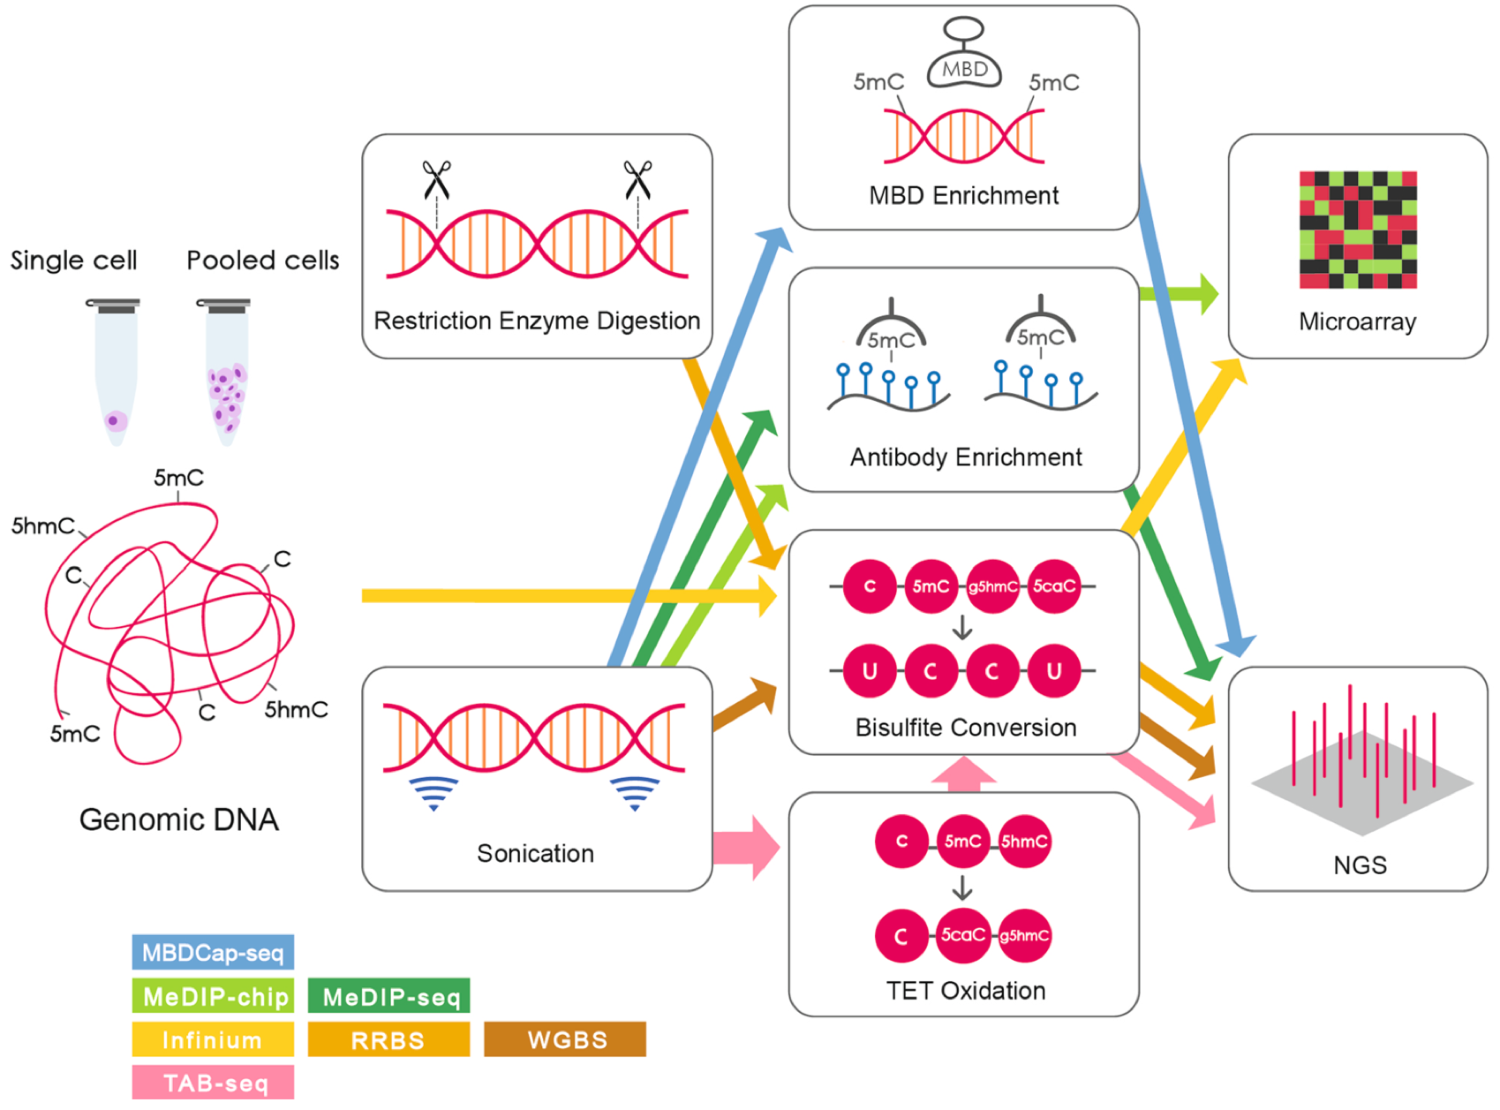
\includegraphics[width=0.8\linewidth]{methylation_protocols}
% 	\caption[]{Workflow of DNA methylation profiling protocols. Reprinted from \cite{Yong2016}}
% 	\label{fig:methylation_protocols}
% \end{figure}

% Alongside scBS, other bulk sequencing methods were also adapted to the single cell resolution, with different trade-offs between coverage and costs. For instance, \cite{Guo2015} adapted the reduced-representation bisulfite sequencing (RRBS-seq) to low starting material by performing all experimental steps before PCR amplification in a single tube. The key principle behind RRBS-seq is to digest the DNA with a restriction endonuclease, followed by a size-selection strategy to enrich for CpG-dense areas \cite{Meissner2005}. This approach significantly reduces sequencing costs at the expense of low coverage in CpG-poor genomic areas, which include repetitive elements, gene bodies and enhancer elements.

\subsubsection{Chromatin accessibility} \label{section:chromatin_accessibility}

In eukaryotes, the genome is packed into a compact complex of DNA, RNA and proteins called chromatin. Several layers of chromatin condensation have been identified, the fundamental unit being the nucleosome, which consists of a string of $\approx$  150bp of DNA wrapped around histone proteins, with linker DNA of $\approx$ 80bp connecting them \cite{Klemm2019,Tsompana2014}. The positioning of the nucleosomes in the nucleus provide an important layer of gene regulation, mostly by exposing or sheltering transcription factor binding sites \cite{Jiang2009}. In general, active regulatory regions tend to have low occupancy of nucleosomes, whereas inactive regions show a high density of nucleosomes \cite{Struhl2013}. Thus, the profiling of DNA accessibility and transcription factor footprints represents an important dimension to understand the regulation of gene expression.

% The N-terminal tails of the histones emerge from the nucleosome and are a strong hotspot for chemical modifications, including methylation, acetylation, phosphorylation and others \cite{Bannister2011}. The complex interaction between a histone modification and the corresponding position, often called the histone code, is an important driver of epigenetic regulation and an active area of research \cite{Zhao2015}.

Traditionally, three main experimental approaches have been used to map bulk chromatin accessibility in a genome-wide and high-throughput manner \cite{Nordstrom2019} (\Cref{fig:ChromatinAcc_protocols}): DNase sequencing (DNase-seq) \cite{Song2010}, transposase-accessible chromatin followed by sequencing (ATAC-seq) \cite{Buenrostro2013} and Nucleosome Occupancy and Methylome-sequencing (NOMe-seq) \cite{Kelly2012}.

\begin{itemize}

	\item \textbf{DNase-seq}: cells are incubated with DNAse I, an enzyme that in low concentrations cuts nucleosome-free regions, hence releasing accessible sites that are subsequently sequenced \cite{Song2010}. Although this methodology became one of the gold standards to map chromatin accessibility by the ENCODE consortium \cite{ENCODE2012,Thurman2012}, it has now been reported that DNase I introduces significant cleavage biases, thus affecting its reliability to infer transcription factor footprints \cite{He2013}.

	\item \textbf{ATAC-seq}: cells are incubated with hyperactive mutant Tn5 transposase, an enzyme that inserts artifical sequencing adapters into nucleosome-free regions. Subsequently, the adaptors are purified, PCR-amplified  and sequenced. In the recent years it has displaced DNase-seq as the \textit{de facto} method for profiling chromatin accessibility due to its fast and sensitive protocol \cite{Buenrostro2015b,Tsompana2014}.

	\item \textbf{NOMe-seq}: follows a very different strategy than the previous technologies. Cells are incubated with a GpC methyltransferase (M.CviPI), which labels accessible (or nucleosome depleted) GpC sites by DNA methylation. In mammalian genomes, cytosine residues in GpC dinucleotides are methylated at a very low rate \cite{Kilgore2007}. Hence, after M.CviPI treatment, GpC methylation marks can be interpreted as direct read outs for chromatin accessibility. \cite{Kelly2012}. NOMe-seq has a range of appealing properties in comparison with count-based methods such as ATAC-seq or DNAseq-seq. First, one can obtain simultaneous information of CpG DNA methylation with little additional cost, permitting the user to effectively measure two molecular layers for the price of one. Second, the resolution of the method is determined by the frequency of GpC sites within the genome ($\approx$ 1 in 16 bp), rather than the size of a library fragment (usually >100 bp). This allows the quantification of nucleosome positioning and transcription factor footprints at high resolution \cite{Kelly2012,Pott2016}. Third, missing data can be easily discriminated from inaccessible chromatin. This implies that lowly accessible sites will not suffer from increased technical variation (due to low read counts) compared to highly accessible sites. The downsides of the approach are the high sequencing depth requirements and the need to discard read outs from GCG positions (21\% of all CG sites) and CGC positions (27\%), as I will discuss later in this thesis.

\end{itemize}


\begin{figure}[H]
	\centering
	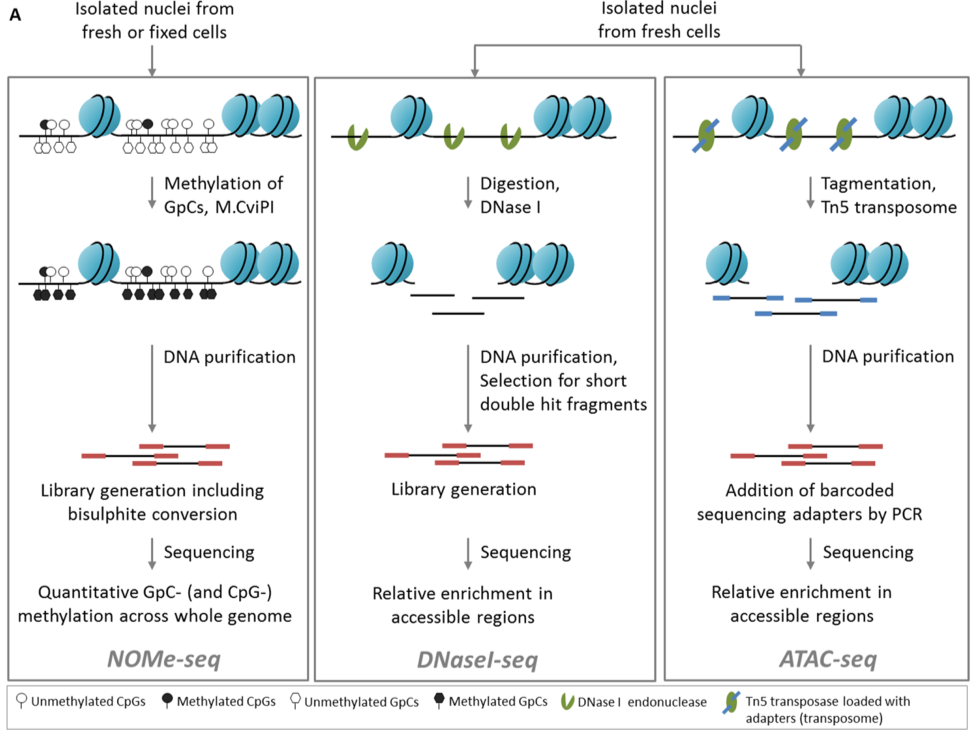
\includegraphics[width=0.75\linewidth]{ChromatinAcc_protocols}
	\caption[]{High-level overview of the workflows for the three main chromatin accessibility assays: NOMe-seq, DNase-seq and ATAC-seq. Reprinted from \cite{Nordstrom2019} with minor modifications.}
	\label{fig:ChromatinAcc_protocols}
\end{figure}

As with DNA methylation, single-cell profiling methods for chromatin accessibility also emerged from its bulk counterparts, including ATAC-seq \cite{Buenrostro2015a}, NOMe-seq \cite{Pott2016} and DNase-seq \cite{Jin2015}. Due to its cost-effective strategy, single-cell ATAC-seq (scATAC-seq) has become the most popular technique to map open chromatin \cite{Cusanovich2015,Cao2018,Chen2018}. Compared to bulk ATAC-seq, scATAC-seq libraries are notably sparse. In a saturated library, \cite{Cusanovich2015} reported a range of $\approx$ 500 to $\approx$ 70,000 mapped reads per cell, with a median of $\approx$ 2500. As the authors report, this represents less than 25\% of the molecular complexity expected from 500-cell bulk experiments. Yet, despite the low coverage, the authors showed that cell-type mixtures can be confidently deconvoluted. Later, in a pioneer effort, \cite{Cusanovich2018b} generated an atlas of chromatin accessibility for different mouse tissues, defining the first \textit{in vivo} landscape of the regulatory genome at single-cell resolution.

\subsection{Multi-modal single-cell sequencing} \label{section:single_cell_multi_modal}

Cellular phenotypes result from the combination of multiple sources of biological information. Undoubtedly, no single "-omics" technology can capture the intricacy of complex molecular mechanisms, but the collective information has the potential to draw a more comprehensive picture of biological processes \cite{Hasin2017,Ritchie2015}.

The profiling of multi-omic readouts at the bulk level is relatively simple, as the same tissue can be dissociated into different aliquots, where each assay can be performed independently \cite{Ritchie2015}. This strategy is also used with single-cell assays, but it has the important downside that the different molecular layers cannot be unambiguously matched, hence limiting the insights that can be inferred from the data. The ultimate goal in single-cell sequencing is to obtain multiple molecular readouts from the same cell, what is termed single-cell multi-omics. The development of these technologies will help us understand the fundamental regulatory principles that connect the different molecular layers. In addition, integrative analyses that simultaneously pool information across multiple data modalities (-omics) and across multiple studies promise to deliver a more comprehensive insights into the complex variation that underlies cellular populations .

Notably, the early success and rapid development of single-cell multi-modal methods has led to their recognition as Method of the year in 2019 by the journal \textit{Nature Methods} \cite{NatMethods2020}. However, their development is still in pilot stages and at the time of writing there is no commercial platform available, limiting its widespread use by the community. As reviewed in \cite{Stuart2019,Chappell2018}, multi-modal measurements can be obtained using three broad strategies:
\begin{itemize}
	
	\item \textbf{Application of a non-destructive assay before a destructive assay}: a prominent example is the sorting of cells based on protein surface markers using (multiparameter) fluorescence-activated cell sorting (FACS) followed by high-throughput sequencing \cite{Paul2015}. Although simple and efficient, this approach requires prior knowledge of protein surface markers, and is limited by the spectral overlap of fluorescence reporters.

	\item \textbf{Physical isolation of different cellular fractions followed by high-throughput sequencing}: this technique was pioneered with the introduction of genome and transcriptome sequencing (G\&T-seq) \cite{Macaulay2015}. After cell lysis, the mRNA fraction is separated from the genomic DNA fraction using biotinylated or paramagnetic oligo(dT) beads, followed by the independent sequencing of the mRNA and the DNA. This strategy allows the simultaneous profiling of transcriptomic measurements with (epi)-genomic measurements, including DNA sequence, copy number variation, DNA methylation or chromatin accessibility \cite{Macaulay2015,Hou2016,Angermueller2016,Hu2016}.

	\item \textbf{Conversion of different molecular layers to a common format that can be measured using the same readout}: prominent examples are the simultaneous measurement of surface proteins and mRNA expression as in Cellular indexing of transcriptomes and epitopes by sequencing (CITE-seq \cite{Stoeckius2017}) and RNA expression and protein sequencing assay (REAP-seq \cite{Peterson2017}). The idea is to incubate cells with antibodies tagged with oligonucleotides that target specific protein surface proteins. This allows both protein surface markers and mRNA levels to be simultaneously measured using a single sequencing round. Notably, this strategy is significantly more powerful than FACS, as the DNA barcodes can be resolved at the sequence level with much higher sensitivity than using fluorescence markers. A second prominent example is NOMe-seq, described in \Cref{section:chromatin_accessibility}. By labelling accessibile GpC sites with DNA methylation marks, one can simultaneously measure endogenous DNA methylation and chromatin accessibility using a single bisulfite sequencing assay.
\end{itemize}

Although single-cell multi-modal have proven successful, they still face numerous difficulties, both from the experimental and the computational front, including limited scalability, low coverage and high levels of technical noise. These difficulties, also inherent to single-cell uni-modal techniques, generally get exacerbated when doing multi-modal profiling. Quoting Cole Trapnell, one of the pioneers of single-cell data analysis: \textit{When you do a multi-omic assay, you're combining all the bad things from multiple protocols} \cite{Eisenstein2020}. A clear example of these challenges is sci-CAR \cite{Cao2018a}, a combinatorial indexing strategy that combines scRNA-seq and scATAC-seq to profile gene expression and chromatin accessibility in the same cell. This is a promising approaches that reported, for the first time, the profiling of both modalities in thousands of cells. However, the  chromatin accessibility modality yielded $\approx$ 10-fold less complexity than (already sparse) scATAC-seq experiments.

I envision that a significant effort will be placed in the next few years to obtain more scalable and cheaper multi-modal measurements from single cells. However, as cost and scalability remain a barrier for high-resolution multi-modal technologies, the development of computational methods that are capable of uncovering biological signal across multiple data modalities while overcoming the technical biases and missing information that are inherent to single-cell experiments, will be a cornerstone of data analysis.


\section{Single-cell data analysis}

From the computational perspective, the rapid development of single-cell technologies has introduced unprecedented challenges for the statistical community, and novel computational methods need to be developed (or adapted) for interrogating the data generated \cite{Stegle2015}. The vast majority of methods are focused on RNA expression, spanning multiple tasks that include normalisation \cite{Lun2016a}, feature selection \cite{Townes2019}, differential expression \cite{Kharchenko2014}, clustering \cite{Kiselev2017}, cell type recognition \cite{Abdelaal2019}, pseudotime inference \cite{Haghverdi2016}, detection of gene regulatory networks \cite{Aibar2017} and batch correction \cite{Haghverdi2018}, among others. Analysis tools have been wrapped into popular platforms such as \textit{Seurat} \cite{Butler2018}, the \textit{Bioconductor} class \textit{SingleCellExperiment} \cite{Amezquita2020} and \textit{Scanpy} \cite{Wolf2018}.

In this section I will provide a brief overview of a typical scRNA-seq analysis pipeline, paying particular attention to the methods that I have used throughout this thesis.

\subsection{Read alignment and gene expression quantification}

The first step in the computational pipeline is to demultiplex the DNA barcodes in order to identify reads that originate from the same cell. This is particularly important when multiple experiments are pooled into a common sequencing library. This task is significantly more complex than in bulk data, owing to the large number of cells and the high rates of errors that can introduce nucleotide missmatches \cite{Tambe2019}.

Subsequently, trimmed reads are aligned to the appropriate reference transcriptome. Gene expression is represented as an integer matrix of counts, with rows representing genomic features (typically genes) and the columns representing individual cells. 

\subsection{Quality control}

Incomplete cell lysis or failures during library preparation may result in poor quality cells that need to be removed for a successful downstream analysis. Typical quality control metrics are the total number of reads detected per cell, the number of genes expressed and the fraction of mitochondrial genes. Cells that are outliers for some of these metrics are filtered out. Importantly, even though there is a generic strategy to assess the quality control for scRNA-seq samples, the specific thresholds vary between data sets and technologies, and care must be taken to always visualise the quality control metrics \cite{Luecken2019}.

A common source of technical variability in single-cell experiments is the existence of doublets, which occurs when multiple cells co-locate in the same well or in the same droplet and are thus assigned the same cell barcode. This results in cells that appear as mixtures of different cellular populations and can be mistaken for non-existing intermediate populations or transitory states.  Thus, it is important to remove doublets so that they do not compromise the downstream analysis. In small-scale plate-based technologies, most doublets can be excluded simply by microscope inspection, but in large-scale droplet-based technologies one needs to adopt data-driven heuristics to exclude multiplet libraries \cite{McGinnis2019}. 


\subsection{Normalisation}

The first step of quality control is essential to remove poor quality cells, but the quality control metrics can vary widely even between cells that pass the filtering criteria. These sources of technical variation arise from any of the library preparation steps, and include PCR amplification biases, differences in RNA capture and reverse transcription efficiency, among others. In addition, the stochasticity of the amplification process produces dropout events, in which no read counts are observed for genes that are expressed \cite{VandenBerge2018}. There has been considerable debate on how to deal with the high proportion of zero counts, and multiple statistical frameworks have been devised, including zero-inflated negative binomial models \cite{Risso2018}. However, recent reports suggest that droplet-based scRNA-seq measurements can be explained by simple Poisson statistics \cite{Svensson2020,Sarkar2020}.

Regardless of the observational model, data normalisation steps are mandatory to eliminate (or at least reduce) the technical variation. Methods that were developed for bulk RNA-seq, including \textit{TMM} \cite{Robinson2010} and \textit{DEseq2} \cite{Love2014} are not successful for scRNA-seq owing to large number of zeros that dominate the gene expression matrix.

In this thesis I adopted the methodology implemented in the \textit{scran} package \cite{Lun2016a}. Briefly, this normalisation procedure divides the gene counts by a size factor per cell and subsequently applies a log transformation with pseudocount on each observation. The essential innovation for single-cell data is to pool expression values from multiple cells (resulting in less zeros) and subsequently deconvolves the cell-specific size factors using a linear system of equations.

Recent works have suggested that global size factors do not effectively normalise all genes at the same time, and different groups of genes require specific size factors in order to remove technical biases \cite{Hafemeister2019}. In this thesis I have not explored this approach, but it showcases how data normalisation is still an open and debated topic in scRNA-seq.

\subsection{Dimensionality reduction}

A key principle of biological data sets is that covariation patterns between the features (i.e. genes) results from differences in underlying processes that can be inferred and interpreted. This key assumption sets off an entire statistical framework of exploiting the redundancy encoded in the data set to reduce the dimensionality of the data in an unsupervised fashion.

Principal Component Analysis (PCA) is the most popular technique for dimensionality reduction of scRNA-seq data \cite{Luecken2019}. A typical analysis pipeline performs clustering, graph inference and other downstream analyses on the (denoised) latent PCA space defined by the top N principal components (where components are ranked by variance explained). Importantly, by maximising the variance explained, PCA implicitly assumes a normal distribution for each feature, and it therefore requires the log transformation above to turn integer counts into continuous measurements. In addition, the log transformation prevents signal being driven by a small number of extremely highly-expressed genes (because in the raw counts the variance of each gene is proportional to its mean expression). 

PCA defines a linear transformation from the high-dimensional space to the low-dimensional space where each component captures an orthogonal source of variation. Capturing the biological signal in most single-cell data sets require a relatively high number of components. Unfortunately, humans do not have the ability to make visual representations of more than three dimensions at the same time, so further dimensionality reduction is typically applied using non-linear techniques, including t-Distributed Stochastic Neighbor Embedding (t-SNE) \cite{vanDerMaaten2008} and Uniform Manifold Approximation and Projection (UMAP) \cite{McInnes2018}. Both methods have been extensively applied, although UMAP is gaining popularity for larger data sets because it preserves better the global structure, whereas t-SNE is largely aimed at preserving local structure. 

\subsection{Clustering}

Unsupervised clustering is arguably one of the most powerful applications of single-cell genomics, as it underpins the ability to define cell types in a coherent, systematic and unbiased manner. Although clustering is still largely empirical and no strong consensus exists on the methodology and the parameters, it is applied in virtually any single-cell data set \cite{Kiselev2019}. The most popular clustering algorithm has traditionally been $k$-means, which iteratively identifies $k$ cluster centroids, and assigns each cell to the nearest centroid. This method is simple, fast and efficient for medium-sized data sets. For large-scale data sets, however, the use of community-detection algorithms on coarse-grained graphs has become more popular \cite{Luecken2019}. Briefly, the first step of commnity-detection methods is to build a k-nearest-neigbourhood graph using a cell-to-cell similarity metric, where each node corresponds to one cell. Then, tighly connected communities are detected by maximising a modularity score, where the modularity quantifies the assignment of nodes to communities when contrasted to a random network.

\subsection{Inference of developmental trajectories}

In many biological systems, and particularly during embryonic development, cells display a continuous spectrum of states where discretisation by clustering may be inappropriate. Due to the destructive nature of single-cell assays, experiments are limited to snapshots and thus are not capable of measuring continuous \textit{real} time. However, differentiating cells are typically asynchronised and display a continuous spectrum of molecular states that reflect the underlying trajectory. Computational methods have been developed to reconstruct this continuity using latent mathematical representations, and are often termed pseudotime methods \cite{Saelens2019}. The aim of pseudotime methods is to generate an ordering of cells according to some metric, which is usually (but not necessarily) some approximation of real time that is inferred from the data. A myriad of pseudotime methods have been developed, with tailored assumptions depending on the nature of the input data and the expected topology of the trajectory (linear, bifurcating, etc.), among other variables \cite{Saelens2019}. 

\section{Integrative analysis of single-cell omics}

Despite the explosion of statistical methods for scRNA-seq data analysis, to date only a few methods have been published with the aim of performing data integration across experiments and data modalities. This is currently defined as one of the grand challenges in single-cell data science \cite{Lahnemann2020}.

\subsection{Defining the common coordinate framework}

The first step when performing data integration is to consider a common coordinate framework to anchor the different data modalities. This defines three broad types of strategies for data integration (\Cref{fig:overview_data_integration}): 

\begin{itemize}

	\item Cells as the common coordinate (\textit{vertical} integration): when the different data modalities are derived from the same cell in \textit{matched} multi-omic assays. This is exemplified by assays such as single-cell Methylome \& Transcriptome (scM\&T-seq) \cite{Angermueller2016}, Cellular Indexing of Transcriptomes and Epitopes by sequencing (CITE-seq) \cite{Stoeckius2017} or Single-nucleus chromatin accessibility and RNA expression sequencing (SHARE-seq) \cite{Ma2020}.

	\item Genomic features as the common coordinate framework (\textit{horizontal} integration): when multiple data modalities of the same type are derived from different subsets of cells. We call this \textit{non-matched} multi-omics and the main advantage is that it is significantly easier and cheaper to obtain than \textit{matched} multi-omics, and as a result most of the current data sets to date belong to this category. An example could be the profiling of scRNA-seq experiments from cells from the same tissue across different groups of donors, where the set of genes represents the anchors.

	\item No common coordinate framework in the high-dimensional space (\textit{diagonal} integration): when both cells and genomic features are different between experiments. This is exemplified by profiling RNA expression and chromatin accessibility from independent sets of cells.

\end{itemize}

\begin{figure}[H]
	\centering
	\includegraphics[width=0.75\linewidth]{overview_data_integration}
	\caption{\textbf{Defining the data integration strategy: choosing the common coordinate framework}.\\Schematic representation of (a) \textit{Horizontal} integration, when features act as anchors (b) \textit{Vertical} integration, when cells act as anchors (c) \textit{Diagonal} integration, when no anchors exist. }
	\label{fig:overview_data_integration}
\end{figure}

\subsection{Challenges of data integration} \label{integrative_analysis_challenges}

The joint analysis of multiple data sources must tackle numerous challenges, some of which are:

\begin{itemize}
	\item \textbf{Heterogeneous data modalities}: measurements collected using different techniques generally exhibit heterogeneous statistical properties and have to be modelled under different statistical assumptions. For example, combining count (i.e. gene expression) and binary traits (i.e.somatic mutations) under the same statistical framework is not a trivial task. In the statistics community, this is commonly refered to as the multi-view learning problem \cite{Xu2013,Li2016}.

	\item \textbf{Overfitting}: as the number of molecular layers increase but the number of samples remain limited, modelling strategies need to account for the risk of overfitting, which can lead to poor generalisation. For example, scM\&T-seq captures the methylation status for potentially millions of CpG sites, but the experimental designs are typically restricted to only a few hundred cells. This is a classic case of a large p and small n problem in high-dimensional statistics, which poses important challenges for most statistical inference procedures.

	\item \textbf{Undesired sources of heterogeneity}: multi-omics data sets typically contain undesired sources of heterogeneity, both technical and biological \cite{Ritchie2015}. Prominent examples are batch effects or cell cycle variation, respectively. If not accounted for, such strong sources of variability can hidden the signal of interest \cite{Buettner2015}. Therefore, understanding and correcting for the underlying principal components of the data represent a critical step before other computational pipelines are applied \cite{Meng2016}.

	\item \textbf{Missing data}: a major problem in some single-cell methodologies is the large amounts of missing information. For example, in a typical single-cell bisulfite experiment less than 10\% of all CpG sites in the genome are measured \cite{Smallwood2014}. This imposes important challenges to some of the conventional statistical methods that do not handle missing information. Furthermore, different assays differ on how missing data is defined. For bisulfite sequencing methods, the missing values are clearly distinguishable from the observed values. However, for other methods such as scRNA-seq or scATAC-seq, the absence of sequence reads do not distinguish between the event that the genomic feature was not measured from that the readout was indeed zero \cite{Clark2018}. Handling of missing information is an important aspect of multi-omics data integration, as some of the standard applications of statistical tools do not handle missing information.

	\item \textbf{Discriminating biological vs technical noise}: multi-omics datasets from relatively complex experimental designs typically contain multiple sources of heterogeneity, both technical and biological. If not accounted for, technical variability can mask biological signal of interest \cite{Buettner2015}. Understanding and correcting technical variation is a critical step to ensure a successful computational analysis.

	\item \textbf{Scalability}: as sequencing costs decrease and technologies improve, we anticipate that multi-modal data sets will follow a similar trend as scRNA-seq, where in the span of less than ten years the size of the experiments ranged from the order of tens to milions of cells \cite{Svensson2018}. The interrogation of exceptionally large data sets requires computational methods to scale accordingly.

	\item \textbf{Noise}: because of the small amounts of starting material, single-cell technologies are inherently noisy and result in large amounts of technical noise \cite{Stegle2015}. Hence, in most cases, inspection of individual genes or cells tends to be unreliable. To overcome this challenge, computational frameworks are required to leverage information on the similarities between cells and/or genes to delinate the signal from noise in order to obtain reliable estimates \cite{Vallejos2015}. Prominent examples are (empirical) Bayesian approaches that are able to borrow information across cells and/or genes and propagate uncertainity when doing inference and predictions \cite{Kharchenko2014}.

	% \item \textbf{Data-driven hypothesis}: the exponential accumulation of biological data is empowering a new type of scientific method where the sheer data itself guides the researcher to formulate specific hypothesis. Importantly, rather than inverting the direction of the scientific method from data to hypothesis, the exploitation of the information hidden in big data sets has the potential to make this relationship bidirectional. Consequently, there is a growing interest in the use of unsupervised methods that, under some specific (hypothesis-driven) assumptions, are able to extract biological insights from the data.

	\item \textbf{Principled validation of the model outputs}: The assessment of data integration outputs is one of the most challenging steps. For most cases, no ground truth is available and one has to assess the model fit by relying on quality control statistics and/or assessing the impact of the integration on downstream analysis tasks (i.e. differential expression, dimensionality reduction, clustering, etc.). The evaluation of the model fit is particularly hard for non-linear methods that can be prone to overfit. 

\end{itemize}

\subsection{Defining the methodology}

Once the common coordinate framework is defined, one needs to choose the data integration strategy. These can fall into two classes: \textit{local} and \textit{global}, a notation inspired from integrative approaches that have been pursued at the bulk level \cite{Ritchie2015}. 

\textit{Local} analyses refer to associations between specific features across different molecular layers, with the aim of detecting putative interactions between them. Prominent examples are associations between genetic variants and gene expression (expression quantitative trait loci, eQTL) or correlations between the epigenetic status of putative regulatory elements and gene expression of nearby genes. The restriction to a local search space is often necessary, to ensure the problem is computationally tractable. For example, cis eQTL mapping is most prevalent because by testing only proximal genetic variants for each gene, the effects of the multiple testing burden is reduced \cite{Nica2013}. Since such association analyses are typically performed per feature (across cells), \textit{local} analyses generally require unambiguous matching between the modalities, as given only by \textit{matched} multi-modal assays, and thus belongs to the category of \textit{vertical} analysis. As for methods, most \textit{local} analyses rely on different flavours of linear regression models, with different modelling assumptions depending on the nature of the molecular readouts. This can include non-gaussian likelihoods, sparsity assumptions to prevent overfitting or probabilistic terms to account for random effects. For example, linear mixed models (LMMs) are a popular framework for performing genetic analyses \cite{Moore2019}. In a LMM, a random effect term is added to account for the population structure and relatedness between individuals, which may affect both the phenotype and the genotype, thus leading to spurious associations if not accounted for.

While useful for characterising genetic variants or identifying putative regulatory elements, \textit{local} analyses have limited capacity to discover complex maps of molecular heterogeneity that result from interactions between genomic features. An alternative strategy for data integration is to exploit the full spectrum of measurements to identify cellular states defined by the coordinated action of multiple genomic elements. For example, cell cycle phase or pluripotency potential are cellular properties that are determined by gene regulatory networks and thus cannot be studied with \textit{local} analyses. \textit{Global} integration is typically (but not always) performed using unsupervised dimensionality reduction approaches that find common modes of variation between molecular layers. Alternatives have been proposed that perform transformations on each data type before merging them into a common similarity network, e.g. using kernel or graph-based approaches \cite{Lanckriet2004, Wang2014}. Nonetheless, both of these approaches have important limitations that will be discussed in this thesis.

Popular examples of global integration methods that have been adapted from the statistical literature are derived as different flavours of matrix factorisation: PCA, Canonical Correlation Analysis (CCA, implemented in Seurat \cite{Butler2018}), Group Factor Analysis (MOFA \cite{Argelaguet2018,Argelaguet2019}, which is introduced in this thesis), Projected Least Squares (PLS, implemented in DIABLO \cite{Singh2018}) and Non-negative Matrix factorisation (NMF, implemented in LIGER \cite{Welch2019}), among others. Although all of these methods share important similarities, the assumptions underlying each model are heavily dependent on the common coordinate framework adopted. As such, the output of each data integration model results from different assumptions and thus has specific challenges and diagnostics that must be addressed accordingly.

\subsubsection{Horizontal integration}

\textit{Horizontal} integration strategies define features as the common anchors in \textit{unmatched} experiments of the same type. This task is faced in most large-scale scRNA projects where data is generated across multiple batches, as uncontrollable differences in the experimental procedure result in systematic deviations in the observed RNA expression (or even cell type composition) across the different batches. If left unaccounted for, these sources of technical variation can mask relevant biological variability and thus complicate the interpretation of the downstream analysis. \textit{Horizontal} integration is currently the most common integrative task, and it is typically regarded as a batch correction problem, where the aim is to remove undesired technical variation across batches while preserving the biological variation contained within each batch \cite{Tran2020}. With the growing availability of reference atlases, epitomised by the Human Cell Atlas project \cite{Aviv2017}, this is arguably one of the most important steps in a single-cell analysis pipeline. 

Linear batch correction methods that were originally developed for bulk datasets such as \textit{limma} \cite{Ritchie2015b} and \textit{ComBat} \cite{Johnson2006}) are not successful for single-cell experiments, mainly because they assume identical (or at least, known) cell type composition across batches. In practice, however, the abundance of cellular subpopulations can vary even between biological replicates due to subtle differences in the library preparation or in the sampling proceudres. As a consequence, the majority of \textit{horizontal} integration methods developed for single-cell data rely on non-linear (or locally linear) strategies that account for differences in cell type compositions.

Several integrative methods have been developed and benchmarked. This includes MNN \cite{Haghverdi2018}, Seurat \cite{Butler2018}, LIGER \cite{Welch2019}, Harmony \cite{Korsunsky2019}, BBKNN \cite{Polanski2019}, scVI \cite{Lopez2018}, Conos \cite{Barkas2019}, among others, which have been benchmarked in an independent study \cite{Luecken2020}. Despite sharing similar principles, these each employ different methodologies. In particular, MNN and Seurat v3 detect mutual nearest neighbors in a joint low-dimensional space, defined by either principal components (MNN) or canonical covariates (Seurat v3). Instead, LIGER performs integrative NMF and disentangles dataset-specific factors versus shared factors, followed by the construction of a neighborhood graph using the shared factors. Harmony learns a cell-specific linear correction function by successive rounds of k-means clustering on a principal component space. BBKNN performs correction on a neighbourhood graph, which results in much faster computations at the expense of losing single-cell resolution. Finally, scVI is a Bayesian variational autoencoder with a probabilistic formulation which includes random variables that account for batch-specific variation.

Most of these methods also share a common set of challenges. First, a classical problem of non-linear integration methods is over-correction, which occurs when the batch correction vector is wrongly estimated and the algorithm forcibly merges non-matching subpopulations of cells \cite{Luecken2020}. This can occur for example when no common axes of biological variation are preserved between the datasets. Second, most methods perform data integration in a denoised latent space, typically using principal components or canonical covariates. This step undoubtedly improves most batch correction algorithms, and is extremely useful for some downstream analysis tasks such as manifold embedding (t-SNE or UMAP plots), graph inference and clustering. However, the high-dimensional observations (i.e. the gene expression counts) can be severely distorted as a result of the batch alignment, and other downstream gene-based analyses such as gene marker detection or differential expression analysis can be problematic \cite{Haghverdi2018}.

\subsubsection{Vertical integration}

\textit{Vertical} integration strategies take advantage of the unambiguous assignment between the molecular profiles in \textit{matched} multi-modal experiments and thus define cells as anchors between data modalities. This facilitates the detection of co-variation patterns across features and permits two data integration strategies: gene-based \textit{local} analysis and a cell-based \textit{global} analysis.

\textbf{Local analysis}

In \textit{local} analyses, the challenge is to distinguish true interactions between features from spurious associations that can result from global confounding effects. To correct for global confounding effects (both technical and biological) affecting the expression phenotype in eQTL mapping, methods such as Principal Component Analysis and PEER \cite{Stegle2010} are often used to identify factors that capture global expression trends, which can be added as covariates in the linear (mixed) model framework. Similarly, the use of a kinship matrix is used to account for global genotype effects that result from population substructure and individual relatedness. Mapping eQTLs using single-cell genomics has led to the identification of cell type-specific eQTL in rare cell populations, which would have been masked using bulk assays \cite{VanDerWijst2018}. Additionally, \cite{Cuomo2020} combined differentiations of iPSCs across multiple donors and single cell expression profiles to show how eQTL influence expression dynamically along a differentiation trajectory. Single cell eQTL mapping is growing as a field, and it promises to provide an extra layer to our understanding of genetic regulation at the molecular level. As methods to assay various molecular traits at single cell resolution become more established, non-expression single cell QTL mapping, where genomic variants are associated with changes in DNA methylation (mQTL), histone modifications (hQTL) or protein (pQTL) level at single cell resolution may also become routine.

\textbf{Global analysis}

% A key principle of biological data is that at least some of the variation observed in the molecular measurements results from differences in underlying, often unobserved, processes. Such processes, whether driven by biological or technical effects, are manifested by coordinated changes in multiple features and thus could be retrieved by learning useful mathematical representations that can be linked to the latent biological processes.

When having a single data modality, PCA is the paradigmatic method for global analysis, and will be discussed in more detail in Chapter 3. Briefly, PCA infers an orthogonal projection of the data onto a low-dimensional space such that the variance explained by the projected data is maximised. The key for the popularity of PCA is its linearity assumption, which ensures that the resulting principal components are simple and interpretable. PCA has also been applied as an integrative method for multi-modal data by extracting principal components from each modality and subsequently comparing them. This approach was attempted in one of the first multi-modal datasets, where scM\&T-seq was used to simultaneously profile RNA expression and DNA methylation on 61 embryonic stem cells \cite{Angermueller2016}. The authors found that a small number of PCs derived from mRNA expression displayed significant correlations with PCs derived from DNA methylation, which suggests that some global sources of variation are preserved across data modalities, but a large fraction of the variation is uncorrelated. This simple analysis provides the intuition for some of the more advanced multi-omic integration methods aimed at performing variance decomposition across data modalities.

An alternative strategy has been to apply PCA after concatenation of the datasets, but this has important limitations when applied to datasets where the features are structured into non-overlapping views (referred to as multi-view data in the machine learning literature). First, PCA extracts components that maximise the variance explained, but it is difficult to quantify the contribution that each component has from each data modality. Second, in its vanilla implementation, PCA does not handle missing values and hence imputation is required when cells do not have measurements available in all data modalities. This is a frequent problem in \textit{matched assays}, as cells might pass quality control for one data modality but not the other. Third, by maximising the variance explained, PCA implicitly assumes a normal distribution for each feature, and is not well suited for the integration of binary and count-based readouts. 

Generalisations of PCA for the integration of multi-omics data have been devised by adapting multi-view learning methods from the statistics literature. Although most of these methods were originally devised for bulk data, the majority of them remain applicable to single-cell multi-modal data. This includes MOFA \cite{Argelaguet2018}, JIVE \cite{Lock2013}, PLS \cite{Singh2018}, MCIA \cite{Meng2014} and iNMF \cite{Welch2019}, all being unsupervised dimensionality reduction methods derived as different flavours of matrix factorisation. As I will discuss in this thesis, the matrix factorisation framework is very appealing due to its simplicity, interpretability, scalability and limited overfitting. Also, it has shown to be an excellent choice for extracting interpretable signatures from sparse and noisy observations such as single-cell measurements.


\subsubsection{Diagonal integration}

The third type of data integration problem is faced when no common coordinate framework exists in the high-dimensional space. This task is faced in \textit{unmatched} experiments when different molecular layers are profiled in different subsets of cells, and is arguably the hardest type of integration. \textit{Diagonal} integration methods are generally aimed at reconstructing a low-dimensional manifold that captures co-variation across data modalities. Thus, a critical assumption of this integrative strategy is the existence of a latent manifold that is shared between the data modalities. For example, this could represent cells sampled from a common differentiation trajectory or cells sampled from a common set of discrete subpopulations.

The simplest strategy that has been employed to solve a \textit{diagonal} integration task is to transform it into a simpler \textit{horizontal} integration task. This can be achieved by summarising molecular measurements over genomic elements that can be unambiguously linked (i.e. RNA expression and promoter methylation). Using this strategy, methods such as LIGER \cite{Welch2019} and Seurat \cite{Stuart2019b} have been successful at integrating unmatched epigenetic and transcriptomic experiments from the same tissue, and even across different species. However, this strategy relies on fragile biological assumptions and is prone to fail in scenarios where molecular layers are not strongly correlated. A good example is early embryonic development where promoter DNA methylation and/or chromatin accessibility are not as predictive of RNA expression \cite{Argelaguet2019} as in terminally differentiated cell types. 

Alternatively, a few methods have attempted to solve this problem by reconstructing technology-invariant integrated latent spaces. The first method to be developed was MATCHER \cite{Welch2017}, a gaussian process latent variable model. However, this method relies upon the strong assumption that biological variation is defined by a unidimensional axis of variation. Some recent methods, including MMD-MA \cite{Liu2019a}, SCIM \cite{Stark2020} and UnionCom \cite{Cao2020} have generalised MATCHER to account for complex multivariate trajectories. However, no independent benchmarking has yet been performed, and the biological insights extracted from these methods have been relatively limited. 


\section{Thesis overview}

In this PhD thesis I sought to develop computational strategies for data integration for single-cell multi-omics. In particular my research focused on the \textit{vertical} integration task, where cells are the common coordinate framework in \textit{matched} assays.

In Chapter 2 I introduce single-cell nucleosome, methylation and transcription sequencing (scNMT-seq), an experimental protocol for the genome-wide profiling of RNA expression, DNA methylation and chromatin accessibility in single cells. While some approaches have reported unbiased genome-wide measurements of up to two molecular layers, scNMT-seq allows, for the first time, the simultaneous profiling of three molecular layers at single cell resolution. We validate the readouts using a simple prototype experiment, and we show how scNMT-seq can be used to study coordinated epigenetic and transcriptomic heterogeneity along a simple differentiation process.

In Chapter 3 I present Multi-Omics Factor Analysis (MOFA), a statistical framework for the integration of multi-omics data sets. MOFA is a latent variable model that offers a principled approach to explore, in a completely unsupervised manner, the underlying sources of sample heterogeneity in a multi-omics data After validating the model features using simulated data, we applied MOFA to a cohort of chronic lymphocytic leukaemia patients. In a quick unsupervised analysis, MOFA revealed the most important dimensions of disease heterogeneity, connected to clinical markers that are commonly used in practice. In a second application we show how MOFA can cope with noisy single-cell multi-modal data, identifying coordinated transcriptional and epigenetic changes along a differentiation process.

In Chapter 4 I discuss how we combined scNMT-seq and MOFA to study the role of epigenetic layers during mouse gastrulation, a critical embryonic stage that spans exit from pluripotency to primary germ layer specification. In this study we built the first triple-omics roadmap of mouse gastrulation, which enabled us to perform an integrative study that revealed novel insights on the dynamics of the epigenome. Notably, we show that cells committed to mesoderm and endoderm undergo widespread epigenetic rearrangements, driven by demethylation in enhancer marks and by concerted changes in chromatin accessibility. In contrast, the epigenetic landscape of ectoderm cells remains in a \textit{default} state, resembling earlier stage epiblast cells. This work provides a comprehensive insight into the molecular logic for a hierarchical emergence of the primary germ layers.

In Chapter 5 I propose an improved formulation of the MOFA framework (MOFA+) aimed at performing integrative analysis of large-scale (single-cell) data sets not only across data modalities but also across independent groups of cells. We introduce key methodological developments, including a fast stochastic variational inference framework and multi-group generalisation in the structure of the prior distributions. All together, this allows MOFA+ to  disentangle heterogeneity across sample groups (i.e. studies or experimental conditions) and data modalities (i.e. omics) in very large data sets. After benchmarking the new features using simulated data, we applied it to single-cell data sets of different scales and designs.

Finally, Chapter 6 summarises this thesis and provides an outlook of future research.


% Chapter 1
%\graphicspath{{Chapter1/Figs/}}

\chapter{Joint profiling of chromatin accessibility DNA methylation and transcription in single cells}

\section{Introduction to single-cell (multi-) omics sequencing}

Next-generation sequencing technologies have revolutionised the study of biological systems by allowing the unbiased profiling of multiple molecular layers, ranging from the genome\cite{Fleischmann1995} and the epigenome\cite{Frommer1992} to the transcriptome\cite{Lister2008,Bainbridge2006,Nagalakshmi2008,Mortazavi2008}. However, bulk sequencing approaches require the pooling of large number of cells to report an average readout, and are hence limited for the study of complex heterogeneous processes, including the immune system, embryonic development or cancer \cite{Griffiths2018,Papalexi2017,Patel2014}.\\
The progressive development of low-input sequencing techniques resulted in an explosion of single-cell sequencing technologies, mostly for the transcriptome (scRNA-seq). In contrast to bulk protocols, single-cell profiling techniques provide an unprecented opportunity to study the molecular variation associated with cellular heterogeneity, lineage diversification and cell fate commitment \cite{Kolodziejczyk2015}.

\subsection{Single-cell RNA sequencing} \label{section:rna_expresssion}
scRNA-seq protocols differ extensively in terms of scalability, costs and sensitivity \cite{Svensson2018, Lafzi2018}. Broadly, there are two groups of methods, plate-based and dropled-based \Cref{fig:scrna_methods}.

In plate-based methods, cells are isolated using micropipettes or flow cytometry into individual wells of a plate, where the library preparation is performed. These class of methods include single-cell tagged reverse transcription sequencing (STRT-seq \cite{Islam2011}), Cell Expression by Linear amplification and Sequencing (CEL-seq \cite{Hashimshony2012}) and Smart-seq\cite{Ramskold2012, Picelli2014}. The main advantage of plate-based methods is the higher quality of libraries and the full length transcript information, in the case of Smart-seq, which enables the quantification of splice variants\cite{Huang2017}, allele-specific fractions\cite{Deng2014} and even RNA velocity information \cite{LaManno2018}. In contrast, the main drawback lies on the low throughput. Yet, multiplexing techniques, the addition of molecular barcodes to cDNA fragments, allow the parallel processing of multiple experiments, thereby increasing the scale of each experiment \cite{Hashimshony2012}.
	
Droplet-based methods are based on the use of droplet microfluidics technology \cite{Zhang2019}. By capturing cells in individual droplets, each containing all necessary reagents for library preparation, this protocol allows the profiling of thousands or even milions of cells in a single experiment. These class of methods include InDrop \cite{Klein2015,Zilionis2016}, Drop-seq\cite{Macosko2015} and the comercial 10x Genomics Chromium \cite{Zheng2017}. All three protocols share similar technologies, including the use of unique molecular identifiers (UMI) to correct for biases in PCR amplifications \cite{Kivioja2011}. Differences lie in the barcode design, cDNA amplification step and bead manufacturing \cite{Zhang2019}. As a trade-off, the increased high throughput of droplet-based approaches comes at the expense of reduced sensitivity\cite{Ziegenhain2017,Wang2019,Svensson2017} (\Cref{fig:scRNA_seq_comparison}).

\begin{figure}[H]
	\centering
	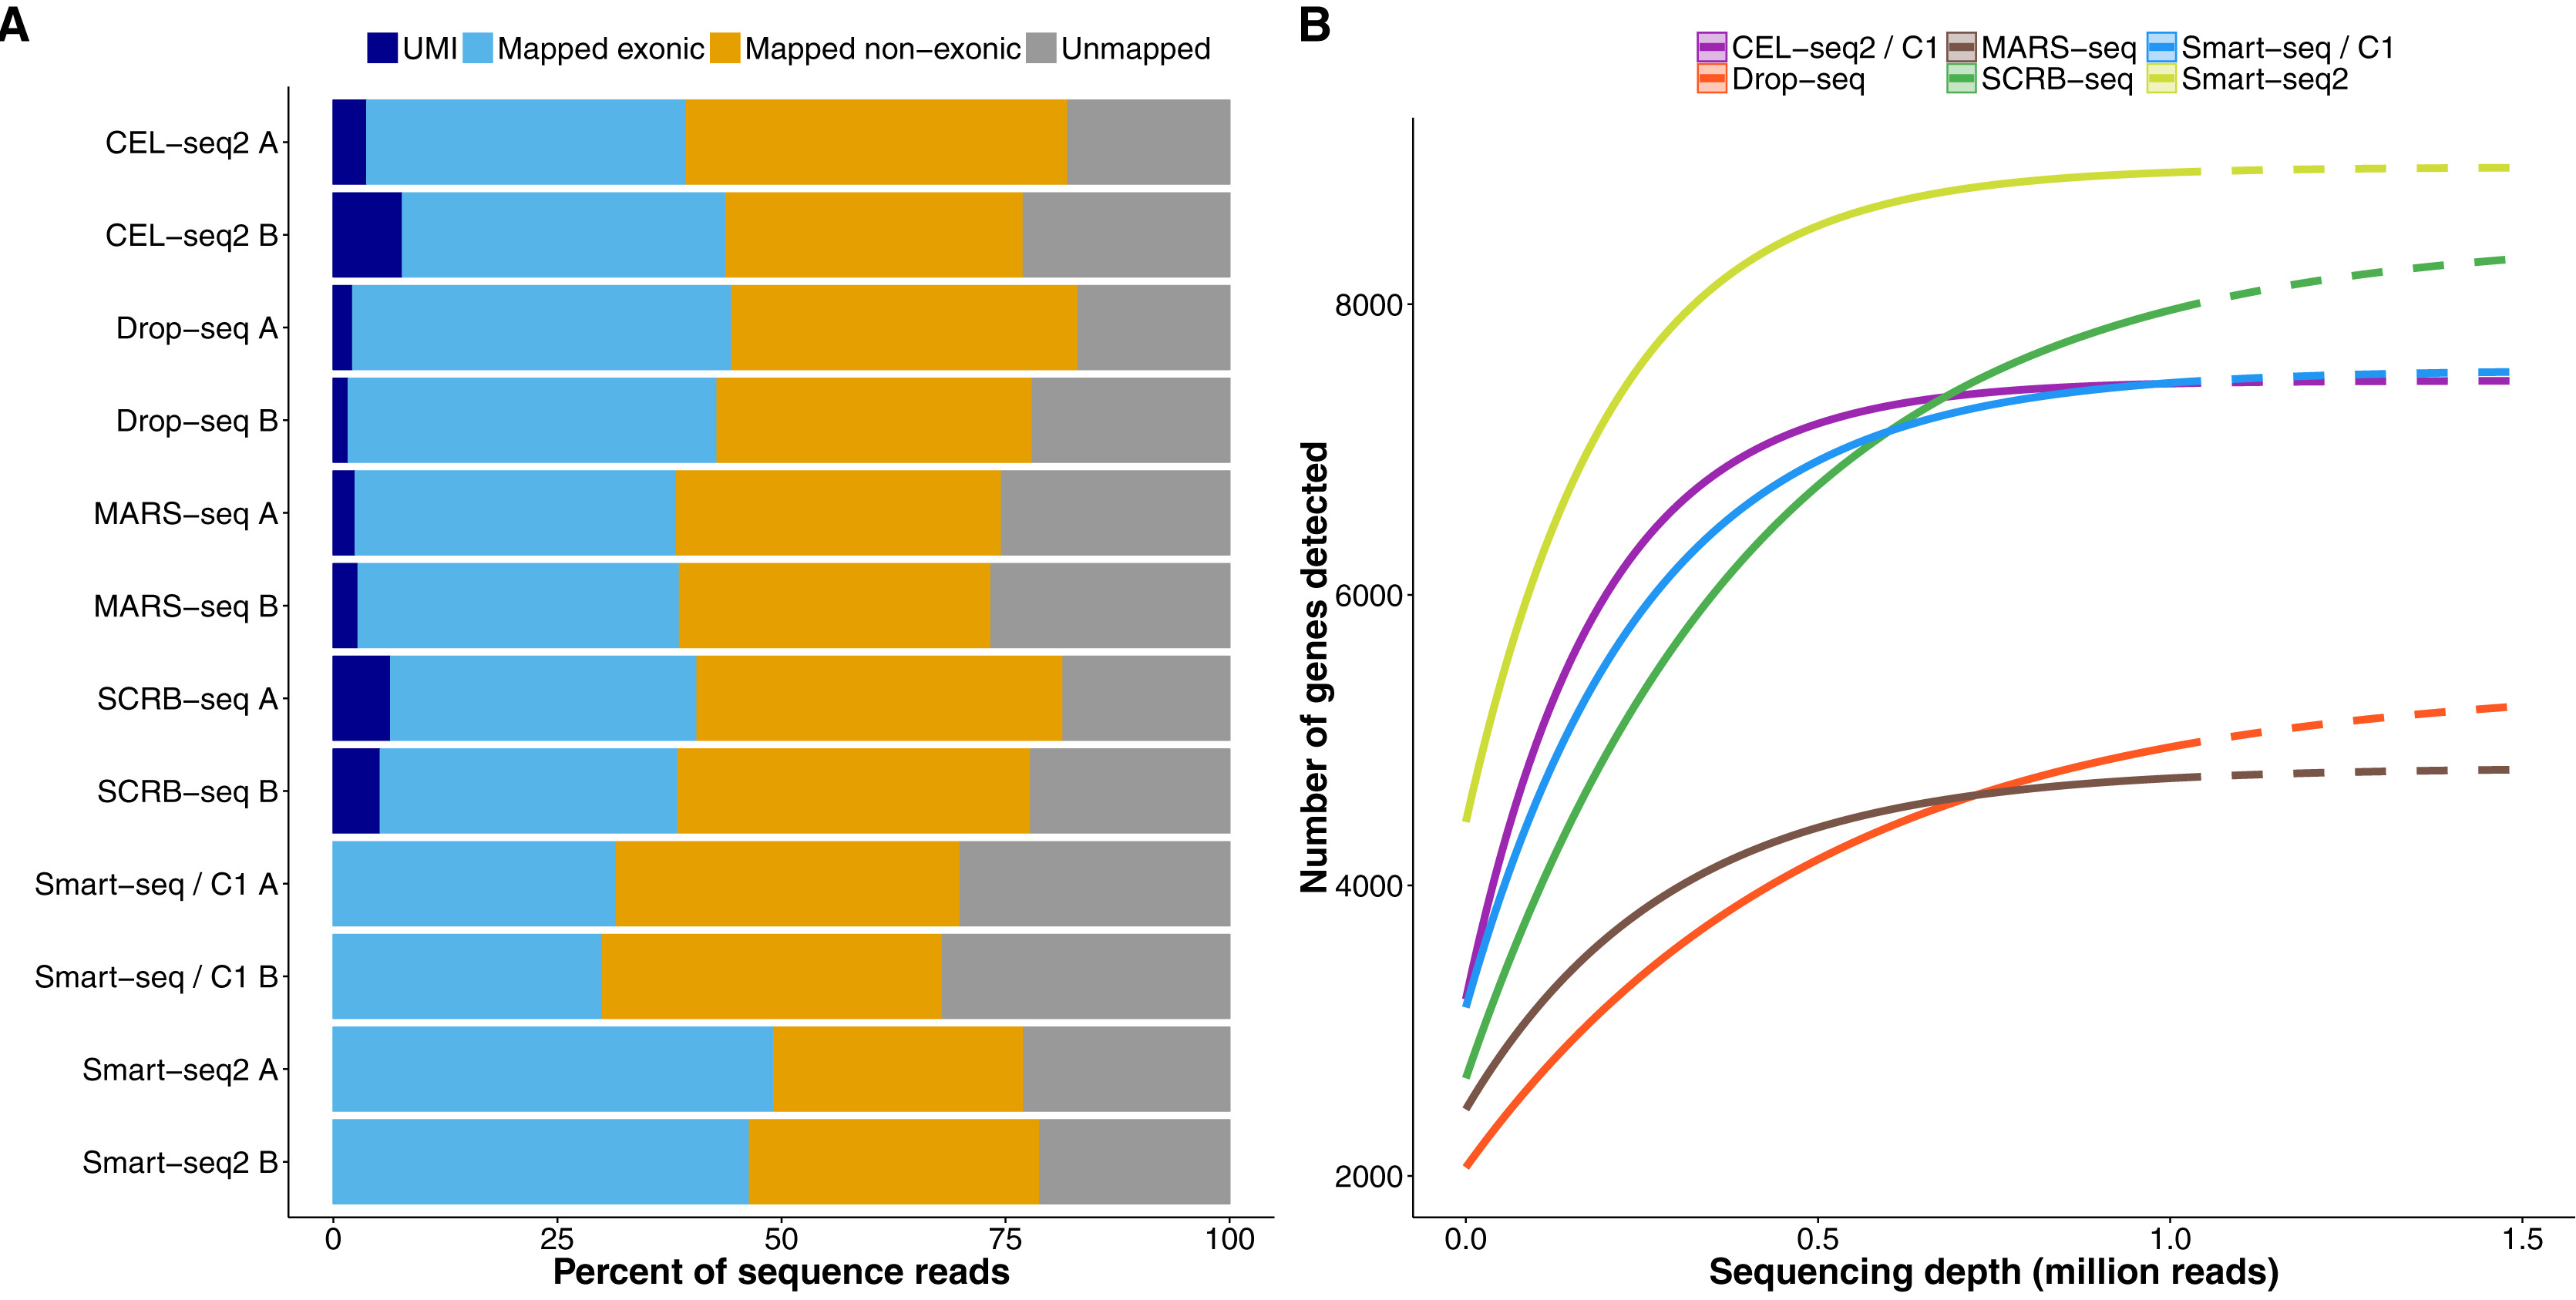
\includegraphics[width=0.85\linewidth]{scRNA_seq_comparison}
	\caption[]{Comparison of quality metrics between different scRNA-seq technologies. (a) Overview of the two types of scRNA-seq methods: plate-based and dropled-based. (b) Fraction of reads mapped to exons (cyan), outside exons (orange) and unmapped (gray). -A and -B denote different replicates. For UMI methods, also shown is the fraction of reads mapping to unique UMIs (dark blue). (c) Median number of genes detected per cell (more than one count) as a function of the (downsampled) sequencing depth. Dashed lines represent extrapolated fits assuming a saturating model. Figure reprinted from \cite{Ziegenhain2017} }
	\label{fig:scRNA_seq_comparison}
\end{figure}

More recently, a third type of scRNA-seq emerged based on a combinatorial cellular indexing strategy \cite{Cao2017,Rosenberg2018}. As demonstrated in a study of mouse organogenesis \cite{Cao2019}, this enables the sequencing of more than a milion cells in a single experiment for a fraction of the cost of other methods. Notably, the same combinatorial indexing strategy has been successfully applied to other data modalities, providing the unprecented opportunity to study multiple molecular layers in an unbiased and high-throughput setting \cite{Vitak2017, Ramani2017, Mulqueen2018}.

\subsection{Single-cell sequencing of the epigenome}

While the large majority of single-cell studies are focused on measuring RNA expression, transcriptomic readouts are just a single dimension of cellular heterogeneity and hence contain limited information to characterise the molecular determinants of phenotypic variation \cite{Ritchie2015}. Consequently, gene expression markers have been identified for a myriad of biological systems, but the accompanying epigenetic changes and the role of other molecular layers in driving cell fate decisions remains poorly understood \cite{Griffiths2018,Kelsey2017,Bheda2014}.

\subsubsection{DNA methylation} \label{section:dna_methylation}
DNA methylation is a stable epigenetic modification that is strongly associated with transcriptional regulation and lineage diversification in both developmental and adult tissues \cite{Jin2018, Harrison2011, Lee2014, Smith2013}. Its classical roles include the silencing of repeating elements, inactivation of the X chromosome, gene imprinting, and repression of gene expression \cite{Jones2012}. Consistently, the disruption of the DNA methylation machinery is associated with multiple dysfunctions, including cancer \cite{Baylin2011}, autoimmune diseases \cite{Liu2013} and neurological disorders \cite{Amir1999}.\\
In mammalian genomes, DNA methylation predominantly occurs at CpG dinucleotides (mCG). The presence of DNA methylation in non-CpG contexts (mCH) has been confirmed, albeit its functional role remains controversial \cite{He2015, Ramsahoye2000, Lister2009}.\\
% The establishment of DNA methylation signatures begin during development by the interplay of \textit{de novo} methylation and demethylation events. In mammals, methylation events are orchestrated by three different DNA methyltransferase enzymes with similar structure but different activity patterns: Dnmt1, Dnmt3a, Dnmt3b.
% Dnmt1 binds hemi-methylated cytosines and is responsible for the maintenance of DNA methylation in replicating cells. In contrast, Dnmt3a and Dnmt3b are known as the de novo methyltransferases and are responsible for establishing the DNA methylation profiles in early development.

Alongisde developments in scRNA-seq technologies, protocols for the profiling of DNA methylation at the single-cell level also emerged from its bulk counterparts (\Cref{fig:methylation_protocols}), notably bisulfite sequencing (BS-seq) \cite{Smallwood2014,Guo2013,Gravina2016,Farlik2015}. The underlying principle of BS-seq is the treatment of the DNA with sodium bisulfite before DNA sequencing, which converts unmethylated cytosine residues to uracil (and eventually to thymine, after PCR amplification), leaving 5-methylcytosine residues intact. The resulting C$\to$T transitions are detected by DNA sequencing, thereby yelding DNA methylation information at single-nucleotide resolution \cite{Frommer1992,Clark2016,Clark2017}.

\begin{figure}[H]
	\centering
	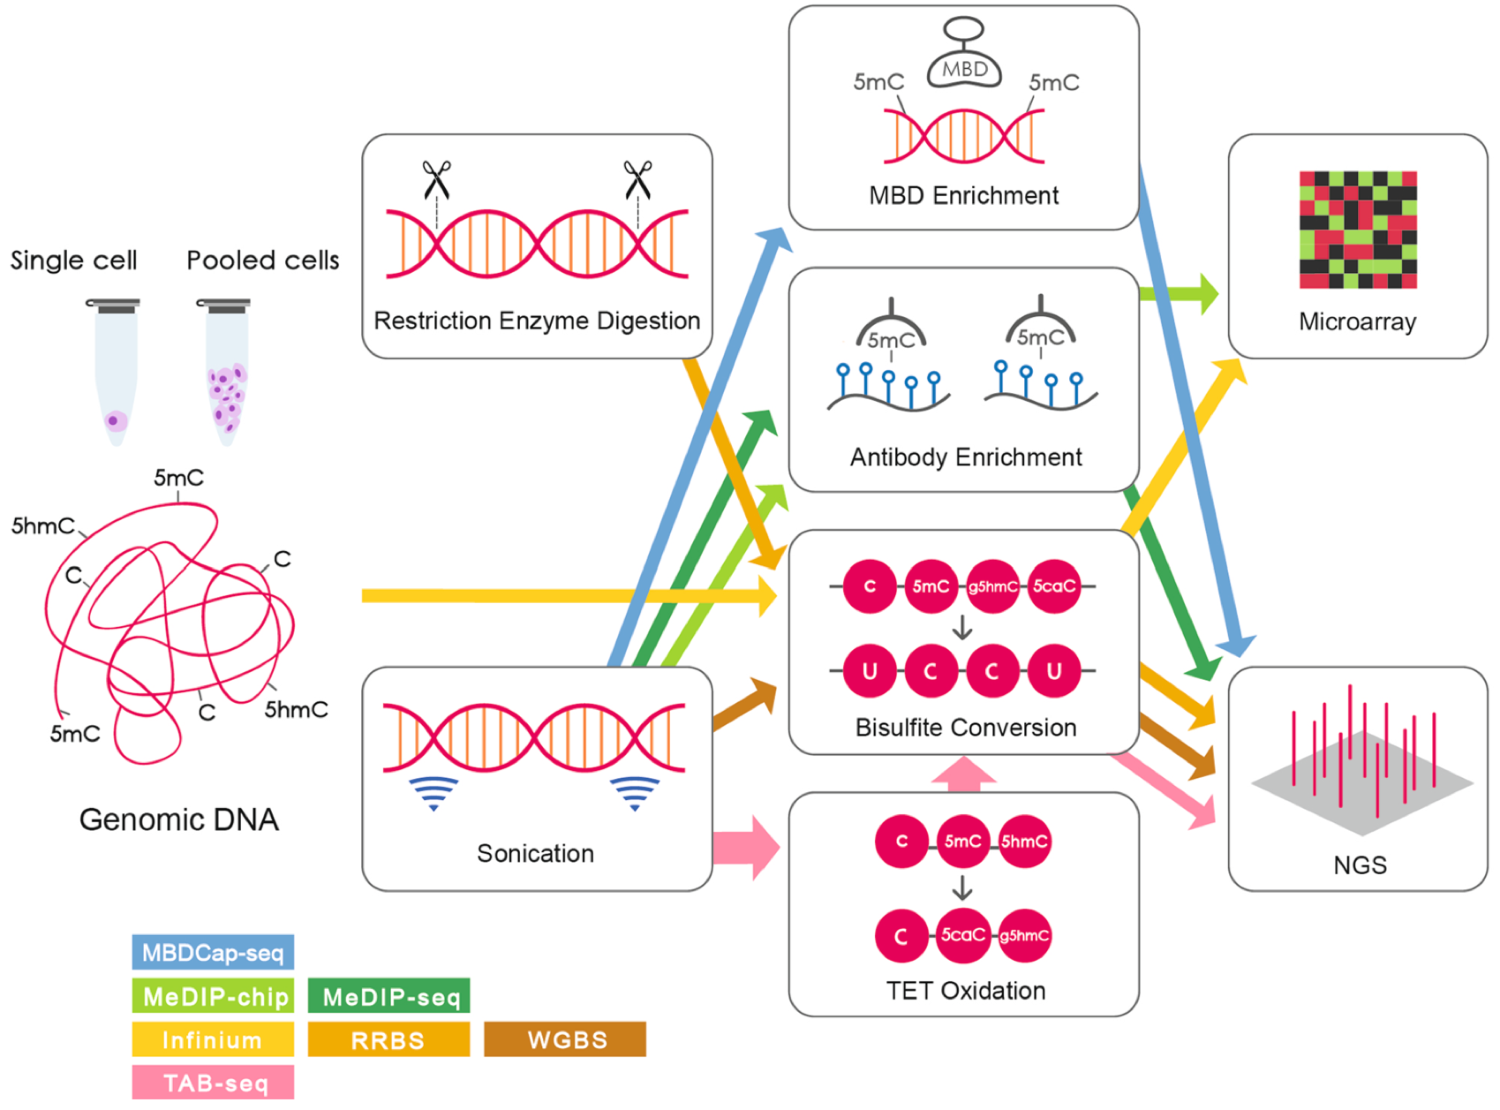
\includegraphics[width=0.8\linewidth]{methylation_protocols}
	\caption[]{Workflow of DNA methylation profiling protocols. Reprinted from \cite{Yong2016}}
	\label{fig:methylation_protocols}
\end{figure}

Nevertheless, the high degree of DNA degradation caused by the purification steps and the bisulfite treatment impaired the use of conventional BS-seq with low starting amounts of DNA. To address this problem, \cite{Smallwood2014} adapted the post-bisulfite adaptor tagging (PBAT) protocol with multiple rounds of 3' random primer amplification (\Cref{fig:scBS}). When the bisulfite treatment is performed before ligation of adaptors, rather than afterwards, loss of adapter-tagged molecules is minimised, hence enabling the use of scBS-seq with little input material.

In a proof of concept study, \cite{Smallwood2014} applied scBS-seq on ovulated metaphase II oocytes (MIIs) and mouse ESCs. They reported an average coverage of 3.7 million CpG dinucleotides (17.7\%) per cell and revealed extensive heterogeneity in the methylome of pluripotent cells.

\begin{figure}[H]
	\centering
	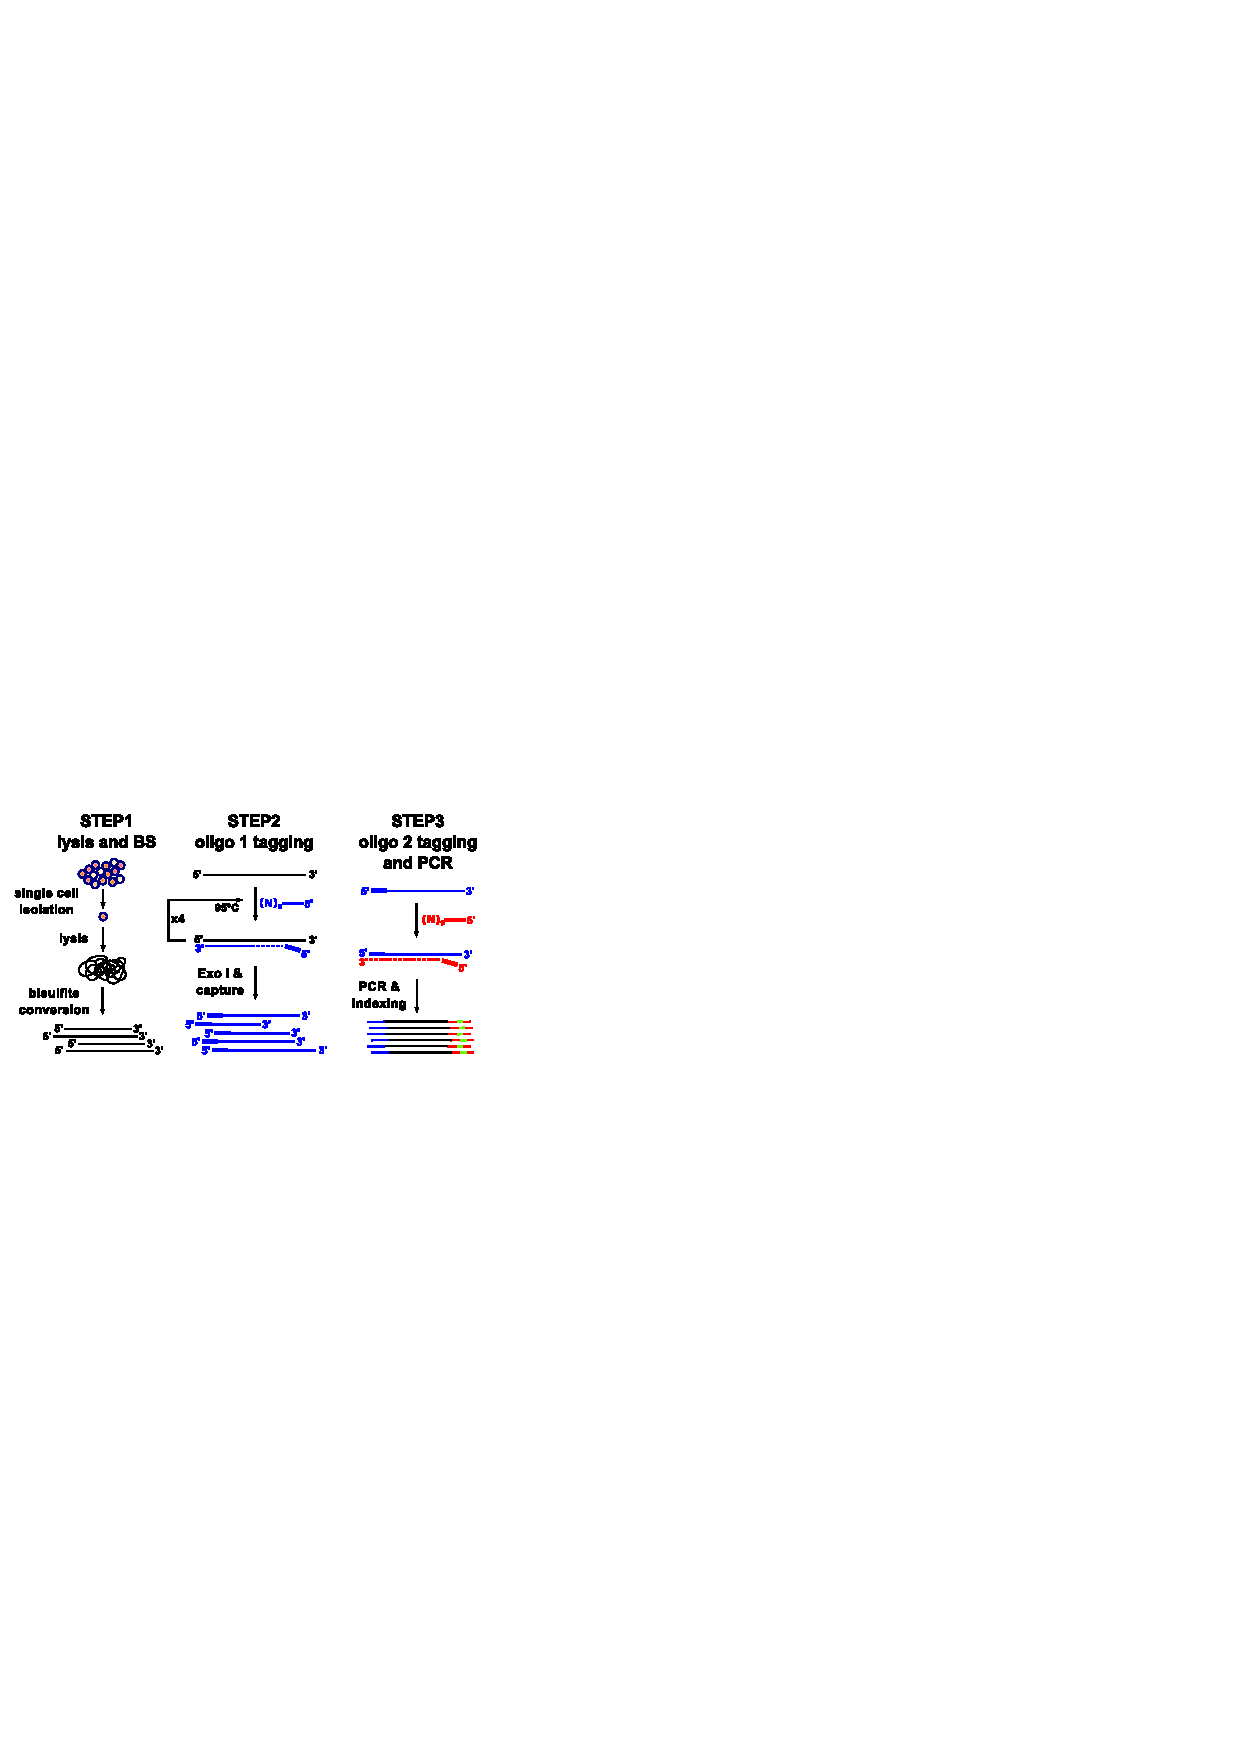
\includegraphics[width=0.8\linewidth]{scBS_protocol}
	\caption[]{scBS-seq profiling protocol. In the first step, cells are isolated and lysed, followed by bisulfite conversion. In the second step, five round of random priming amplification are performed using the first sequencing adaptor. In the third step, this process is repeated using the second sequencing adaptor. Finally, the resulting fragments are PCR-amplified and sequenced. Figure reprinted from \cite{Smallwood2014}.}
	\label{fig:scBS}
\end{figure}

Alongside scBS, other bulk sequencing methods were also adapted to the single cell resolution, with different trade-offs between coverage and costs. For instance, \cite{Guo2015} adapted the reduced-representation bisulfite sequencing (RRBS-seq) to low starting material by performing all experimental steps before PCR amplification into a single tube. The key principle behind RRBS-seq is to digest the DNA with a restriction endonuclease, followed by a size-selection strategy to enrich for CpG-dense areas \cite{Meissner2005}. This approach significantly reduces sequencing costs at the expense of low coverage in CpG-poor genomic areas, which include repetitive elements, gene bodies and enhancer elements \cite{Martin-Herranz2017}.\\

(IMPROVE) More recently, combinatorial indexing technologies such as sci-MET \cite{Mulqueen2018} and snmC-seq \cite{Luo2018} enabled the profiling of thousands of single cells in parallel, increasing the highthroughput, albeit yelding lower coverage than scBS-seq (maximum of 7.0\% observed CpG sites) \cite{Mulqueen2018}. The idea behind the combinatorial indexing strategy is to tag the DNA with multiple adaptors such that the probability of two cells harboring the same adatpor is very low. This allows a large range of cells to be processed in parallel, significantly increasing the cell count throughput. Additionally, the proposed combinatorial indexing techniques yield higher mapping rates, on the order of 60\% \cite{Mulqueen2018} compared to 30\% in scBS-seq \cite{Smallwood2014}. 
% 	snmC-seq2 is not combinatorial indexing. it is essentially an optimised and automated version of scBS

\subsubsection{Chromatin accessibility} \label{section:chromatin_accessibility}
In eukaryotes, the genome is packed into a compact complex of DNA, RNA and proteins called chromatin. Several layers of chromatin condensation have been identified, the fundamental unit being the nucleosome, which consists on a string of $\approx$  150bp of DNA wrapped around histone proteins, with linker DNA of $\approx$  80bp connecting them \cite{Klemm2019,Tsompana2014}. The N-terminal tails of the histones emerge from the nucleosome and are a strong hotspot for chemical modifications, including methylation, acetylation, phosphorylation and others \cite{Bannister2011}. The complex interaction between a histone modification and the corresponding position, often called the histone code, is an important driver of epigenetic regulation and an active area of research \cite{Zhao2015}.

In addition to the histone modifications, the positioning of the nucleosomes provide another layer of gene expression regulation, mostly by exposing or sheltering transcription factors binding sites \cite{Jiang2009}. In general, active regulatory regions tend to have low occupancy of nucleosomes, whereas inactive regions show a high density of nucleosomes \cite{Struhl2013}. Thus, the profiling of DNA accessibility and transcription factor footprints represents an important dimension to understand the regulation of gene expression.

Traditionally, four main experimental approaches have been used to map chromatin accessibility in a genome-wide and high-throughput manner (\Cref{fig:ChromatinAcc_protocols}): MNase sequencing (MNase-seq) \cite{Kaplan2008}, DNase sequencing (DNase-seq) \cite{Song2010}, transposase-accessible chromatin followed by sequencing (ATAC-seq) \cite{Buenrostro2013} and Nucleosome Occupancy and Methylome-sequencing (NOMe-seq) \cite{Kelly2012}. A systematic comparison with a controlled experimental design can be found in \cite{Nordstrom2019}.

\begin{itemize}

	\item \textbf{MNase-seq}: the chromatin is incubated with a micrococcal nuclease (MNase), an enzyme that degrades naked DNA, followed by purification, adapter ligation, PCR amplification and next-generation sequencing. As nucleosomes protect the DNA from digestion, the resulting sequencing fragments reveal nucleosome location, hence providing an inverse measure of chromatin accessibility \cite{Kaplan2008}.

	\item \textbf{DNase-seq}: the chromatin is incubated with DNAse, an enzyme that in low concentrations cuts nucleosome-free regions. Hence accessible sites, typically called DNase I hyper-sensitive sites, are released and sequenced \cite{Song2010}. In contrast to MNase-seq, this assay provides a direct measure of chromatin accessibility, and became one of the gold standards to map chromatin accessibility in the human genome by the ENCODE consortium \cite{ENCODE2012,Thurman2012}. However, it has been reported that DNase I introduces significant cleaveage biases, thus affecting its reliability to infer transcription factor footprints \cite{He2013}.

	\item \textbf{ATAC-seq}: the chromatin is incubated with hyperactive mutant Tn5 transposase, an enzyme that inserts artifical sequencing adapters into nucleosome-free regions. Subsequently, the adaptors are purified, PCR-amplified  and sequenced. As in DNase-seq, it provides a direct measure of chromatin accessibility. Yet, in the last years it has arguably displaced DNase-seq or MNase-seq as the \textit{de facto} method for profiling chromatin accessibility due to its fast and sensitive protocol \cite{Buenrostro2015b,Tsompana2014,Nordstrom2019}.

	\item \textbf{NOMe-seq}: it follows a very different strategy than the previous technologies. The idea is to incubate cells with a GpC methyltransferase (M.CviPI), which labels accessible (or nucleosome depleted) GpC sites by DNA methylation. In mammalian genomes, cytosine residues in GpC dinucleotides are methylated at a very low rate \cite{Kilgore2007}. Hence, after M.CviPI treatment and bisulfite sequencing, GpC methylation marks can be interpreted as direct read outs for chromatin accessibility, as opposed to the CpG methylation readouts, which can be interpreted as endogenous DNA methylation marks \cite{Kelly2012}.
	NOMe-seq has a range of appealing properties in comparison with count-based methods such as ATAC-seq or DNAseq-seq. First, the obvious gain of simultaneously measuring another epigenetic readout such as DNA methylation with little additional cost. Second, the resolution of the method is determined by the frequency of GpC sites within the genome ($\approx$ 1 in 16 bp), rather than the size of a library fragment (usually >100 bp). This allows the robust inspection of individual regulatory elements, nucleosome positioning and transcription factor footprints \cite{Kelly2012,Pott2016,Nordstrom2019}. Third, missing data can be easily discriminated from inaccessible chromatin. Importantly, this implies that lowly accessible sites will not suffer from increased technical variation (due to low read counts) compared to highly accessible sites. Finally, the M.CviPI enzyme shows less sequence motif biases than the DNAse or the Tn5 transposase \cite{Nordstrom2019}.
	The downsides of the approach are the high sequencing depth requirements and the need to discard read outs from GCG positions (21\%) and CGC positions (27\%).	

\end{itemize}



\begin{figure}[H]
	\centering
	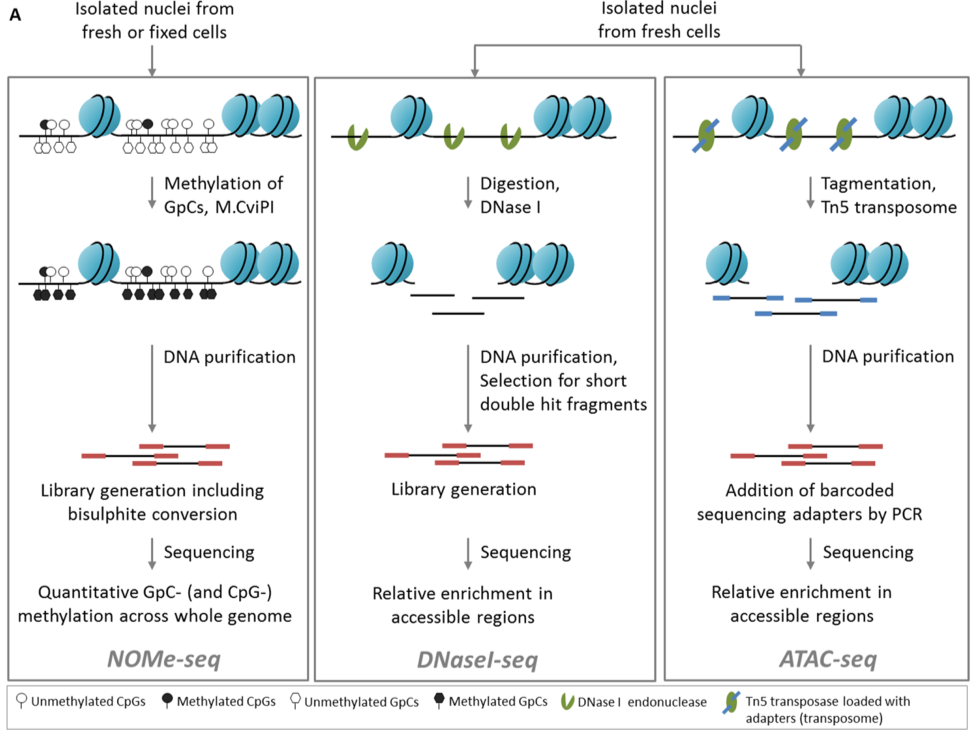
\includegraphics[width=0.8\linewidth]{ChromatinAcc_protocols}
	\caption[]{High-level overview of the workflows for the three main chromatin accessibility assays: NOMe-seq, DNase-seq and ATAC-seq. Reprinted from \cite{Nordstrom2019}. }
	\label{fig:ChromatinAcc_protocols}
\end{figure}

As with DNA methylation, single-cell profiling methods for chromatin accessibility also emerged from its bulk counterparts, including ATAC-seq\cite{Buenrostro2015a}, NOMe-seq \cite{Pott2016} and DNase-seq \cite{Jin2015}.

Due to its cost-effective strategy, single-cell ATAC-seq has become the most established technique to map open chromatin regions, revealing extensive heterogeneity across different cellular populations \cite{Cusanovich2015,Cao2018,Chen2018}. 

Compared to bulk ATAC-seq, scATAC-seq libraries are notably sparse. In a satured library, \cite{Cusanovich2015} reported a range of $\approx$ 500 to $\approx$ 70,000 mapped reads per cell, with a median of $\approx$ 2500. This represents less than 25\% of the molecular complexity expected from 500-cell bulk experiments. Yet, despite the low coverage, they showed that cell-type mixtures can be confidently deconvoluted. Later, in a pioneer effort, \cite{Cusanovich2018b} generated an atlas of chromatin accessibiliy for different mouse tissues, defining the first \textit{in vivo} landscape of the regulatory genome single-cell resolution.

However, the sparse nature of scATAC-seq makes it impractical for the study of heterogeneity in individual regulatory elements. This is addressed mostly by NOMe-seq, which at the expensive of more expensive sequencing and limited scalability, it provides base-pair resolution readouts, even at the single cell resolution \cite{Pott2016}.


\subsection{Multi-modal single-cell sequencing}
Cellular phenotypes have been historically characterised using exploratory methods in single molecular layers, most commonly the transcriptome. However, phenotypes result from the combination of multiple sources of biological information, including the genetic background, epigenetic marks, protein levels or lipid composition. Undoubtedly, no single "-omics" technology can capture the intricacy of complex molecular mechanisms, but the collective information has the potential to draw a more comprehensive picture of biological processses as well as clinically relevant traits \cite{Hasin2017,Ritchie2015}.\\
Motivated by this assumption, multiple omics are being increasingly applied across a wide range of biological domains, including cancer biology \cite{Akavia2010,Gerstung2015}, regulatory genomics \cite{Chen2016}, microbiology \cite{Kim2016} or host-pathogen interactions \cite{Soderholm2016}.

Recent technological advances have enabled the profiling of multiple omics in the same single cell, which has the potential to provide a more comprehensive understanding of biological processess, including mechanistic relationships between the (epi)genome and the transcriptome.\\
Multi-modal sequencing technologies are becoming rapidly available and its explosion is likely to mirror the trend of scRNA-seq technologies. As reviewed in \cite{Stuart2019,Chappell2018}, multi-modal measurements can be obtained using four broad strategies:
\begin{itemize}
	
	\item \textbf{Application of a non-destructive assay before a destructive one}: the most prominent example is multiparameter fluorescence-activated cell sorting (FACS) followed by destructive high-throughput sequencing \cite{Paul2015}. Although simple and efficient, this approach requires prior knowledge of gene expression markers to sort the populations of interest and is limited by the spectral overlap of fluorescence reporters.

	\item \textbf{Physical isolation of different cellular fractions followed by independent high-throughput sequencing}: this technique was pioneered with the simultaneous genome and transcriptome sequencing (G\&T-seq) \cite{Macaulay2015}. After cell lysis, the mRNA fraction is separated from the genomic DNA fraction using biotinylated or paramagnetic oligo(dT) beads, followed by conventional uni-modal sequencing of the mRNA and the DNA. This strategy allows the simultaneous profiling of transcriptomic measurements with genome-derived measurements, including DNA sequence, copy number variation, DNA methylation or chromatin accessibility \cite{Macaulay2015,Hou2016,Angermueller2016,Hu2016}\\
	A clear advantage of this methodology is its unsupervised nature, which makes it particularly useful for the study of tissues with complex heterogeneity.

	\item \textbf{Conversion of different molecular layers to a common format that can be simultaneously measured using the same readout}: this represents a powerful methodology, as it allows multiple modalities to be profiled in a single workflow. Prominent examples are the simultaneous measure of surface proteins and mRNA expression as in Cellular indexing of transcriptomes and epitopes by sequencing (CITE-seq\cite{Stoeckius2017}) and RNA expression and protein sequencing assay (REAP-seq\cite{Peterson2017}). The idea is to incubate cells with antibodies tagged with oligonucleotides that target specific proteins. Subsequently, additional barcodes are introduced for PCR amplification and a poly(A)-tail selection step is performed, allowing the simultaneous pooling of mRNAs (cDNAs) and antibody tags. Finally, After PCR amplification, both types of molecules can be separated by size and sequenced.\\
	In practice, this principle is significantly more powerful than FACS, as the DNA barcodes can be resolved with very high sensitivity by sequencing and their complexity is limited by the number of nucleotides ($4^N$ where $N$ is the length of the barcode)\\
	A second prominent example is NOMe-seq, described in \Cref{section:chromatin_accessibility}. By labelling accessibile GpC sites with DNA methylation marks, one can simultaneously measure endogenous DNA methylation and chromatin accessibility using a single bisulfite sequencing assay.
\end{itemize}
	% MENTION SI-CAR
	% MENTION SPATIAL DATA
Combinations of the three approaches above have also been achieved. One of them, single-cell nucleosome, methylome and transcriptome (scNMT-seq\cite{Clark2018}), which is presented in this thesis, combines the principle of physical isolation with the conversion to a common format to achieve a simultaneous measurement of three molecular layers.

Although they have been proven successful, single-cell multi-modal approaches still face numerous difficulties, both from the experimental and the computational side, including limited scalability, low coverage and high levels of technical noise. These difficulties, also inherent to single-cell uni-modal techniques, generally get exacerbated when doing multi-modal profiling. A clear example is scNMT-seq, where an almost \%50 decrease of coverage is observed in DNA methylation with respect to scM\&T-seq. Similarly, chromatin accessible measurements in sci-CAR\cite{Cao2018a} showed \~10-fold less complexity than scATAC-seq.\\
As cost and limited scalability will likely remain the main barrier for high-resolution multi-modal technologies, we expect novel strategies to be aimed at exploiting the rich amount of information by merging or mapping the multi-modal data sets to large uni-modal atlases \cite{Aviv2017,Cao2019,Cusanovich2018b,Pijuan-Sala2019}.\\
Computational challenges and strategies in multi-modal data will be discussed in Chapters 2 and 4.
	% Astonishing sentence to finish



%\graphicspath{{Chapter1/Figs/}}

\section{Joint profiling of chromatin accessibility, DNA methylation and RNA expression in single cells}

\subsection{Description of the experimental protocol} \label{section:scnmt_protocol}

scNMT-seq builds upon two previous multi-modal protocols: single-cell Methylation and Transcriptome sequencing (scM\&T-seq) \cite{Angermueller2016} and Nucleosome Occupancy and Methylation sequencing (NOMe-seq) \cite{Kelly2012,Pott2016}. An overview of the protocol is shown in \Cref{fig:scnmt_protocol}.

In the first step (the NOMe-seq step), cells are sorted into individual wells and incubated with a GpC methyltransferase (M.CviPI). This enzyme labels accessible (or nucleosome depleted) GpC sites via DNA methylation\cite{Kilgore2007, Kelly2012}. In mammalian genomes, cytosine residues in GpC dinucleotides are methylated at a very low rate. Hence, after M.CviPI treatment, GpC methylation marks can be interpreted as direct read outs for chromatin accessibility, as opposed to the CpG methylation readouts, which can be interpreted as endogenous DNA methylation\cite{Kilgore2007, Kelly2012}.

In a second step (the scM\&T-seq step), the DNA molecules are separated from the mRNA using oligo-dT probes pre-annealed to magnetic beads. Subsequently, the DNA fraction undergoes single-cell bisulfite conversion\cite{Smallwood2014}, whereas the RNA fraction undergoes Smart-seq2 \cite{Picelli2014}.\\

\begin{figure}[H]
	\centering
	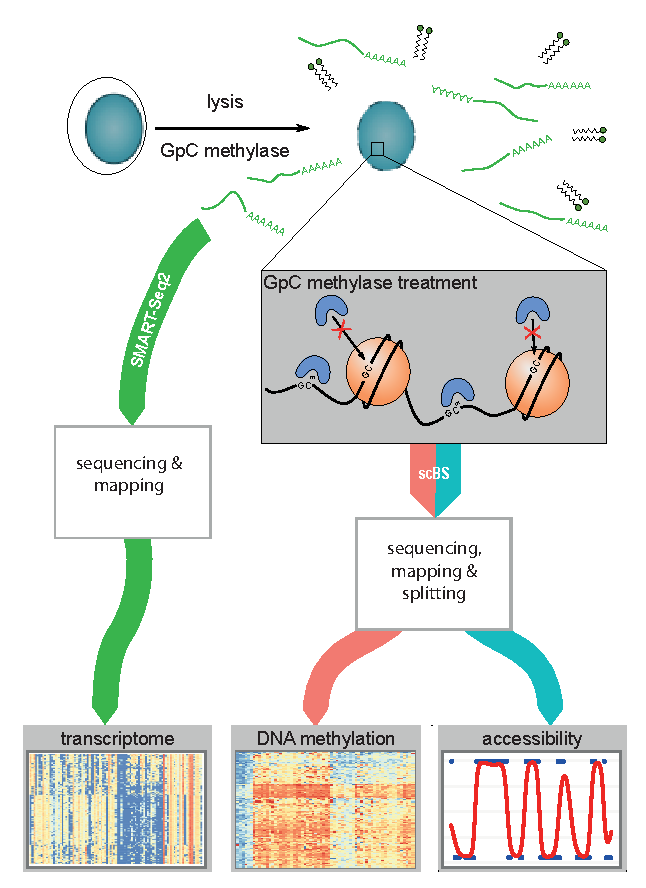
\includegraphics[width=0.55\linewidth]{scNMT_protocol}
	\caption[]{\textbf{scNMT-seq protocol overview.}\\
	In the first step, cells are isolated and lysed. Second, cells are incubated with a GpC methyltransferase. Third, the RNA fraction is separated using oligo-dT probes and sequenced using Smart-seq2. The DNA fraction undergoes scBS-seq library preparation and sequencing. Finally, CpG Methylation and GpC chromatin accessibility data are separated computationally.}
	\label{fig:scnmt_protocol}
\end{figure}

As discussed in \Cref{section:chromatin_accessibility}, NOMe-seq has a range of appealing properties in comparison with count-based methods such as ATAC-seq or DNAseq-seq. First, the obvious gain of simultaneously measuring another epigenetic readout such as DNA methylation with little additional cost. Second, the resolution of the method is determined by the frequency of GpC sites within the genome ($\approx$ 1 in 16 bp), rather than the size of a library fragment (usually >100 bp). This allows the robust inspection of individual regulatory elements, nucleosome positioning and transcription factor footprints \cite{Kelly2012,Pott2016,Nordstrom2019}. Third, missing data can be easily discriminated from inaccessible chromatin. Importantly, this implies that lowly accessible sites will not suffer from increased technical variation (due to low read counts) compared to highly accessible sites. Finally, the M.CviPI enzyme shows less sequence motif biases than the DNAse or the Tn5 transposase \cite{Nordstrom2019}.

The downsides of the approach are the limited scalability associated with plate-based methods, and the need to discard read outs from (1) GCG positions (21\% of all CpG sites), as it is intrinsically not possible to distinguish endogenous methylation from \textit{in vitro} methylated bases, and (2) CGC positions (27\%), to mitigate off-target effects of the enzyme \cite{Kelly2012}. This filtering step reduces the number of genome-wide cytosines that can be assayed from 22 million to 11 million. 


\subsection{Description of the data processing pipeline}

After DNA sequencing, reads undergo quality control and trimming using TrimGalore to remove the flanking 6bp (the random primers), adaptor contamination and poor-quality base calls. Subsequently, trimmed reads are aligned to the corresponding genome assembly. Here we used Bismark \cite{Krueger2011} with the additional --NOMe option, which produces CpG report files containing only ACG and TCG trinucleotides and GpC report files containing only GCA, GCC and GCT positions.

Following \cite{Smallwood2014}, a bernoulli model is assumed for each CpG and GpC site in each cell after removal of duplicate alignments, which results in binary methylation calls. Notice that the use of a bernoulli model is an exclusive property of single-cell bisulfite sequencing data, for the vast majority of sites only one allele is observed per cell (due to data sparsity). This contrasts with bulk bisulfite sequencing data, where each dinucleotide typically contains multiple reads (originating from different cells) and thus a binomial model is more appropriate than a bernoulli estimate.

Finally, when quantifying DNA methylation and chromatin accessibility over genomic features (i.e. promoters or enhancers) a binomial model is assumed for each cell and feature, where the number of successes is the number of methylated CpGs (or GpCs) and the number of trials is the total number of CpGs (or GpCs) that are observed within the specific cell and genomic feature.

\subsection{Data validation}

\subsubsection{Coverage} \label{section:scnmt_coverage}

We validated scNMT-seq in 70 EL16 mouse embryonic stem cells (ESCs), together with 3 cells processed without M.CviPI enzyme treatment (i.e. using scM\&T-seq). The use of this relatively simple and well-studied \textit{in vitro} system allows us to compare our DNA methylation and chromatin accessibility statistics to published data \cite{Smallwood2014,Angermueller2016,Ficz2013}.

First, we compared the theoretical maximum coverage that could be achieved with the empirical coverage (\Cref{fig:scnmt_coverage}). Despite the reduction in theoretical coverage due to the removal of ambiguous CCG and GCG sites, we observed, for DNA methylation, a median of $\approx$ 50\% of promoters, $\approx$ 75\% of gene bodies and $\approx$ 25\% of active enhancers captured by at least 5 CpGs in each cell. Nevertheless, limited coverage is indeed observed for small genomic contexts such as p300 ChIP-seq peaks (median of $\approx$ 200bp).\\
For chromatin accessibility, coverage was larger than that observed for endogenous methylation due to the higher frequency of GpC dinucleotides, with a median of $\approx$ 85\% of gene bodies and $\approx$ 75\% of promoters measured with at least 5 GpCs.

\begin{figure}[H]
	\centering
	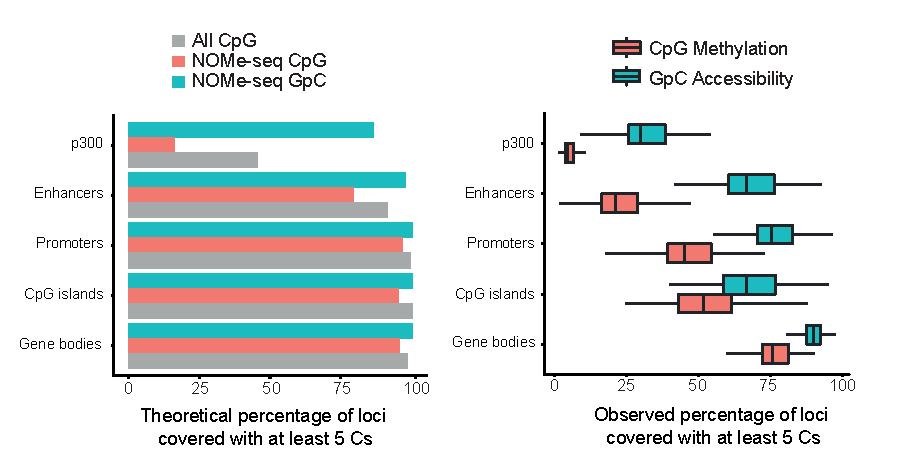
\includegraphics[width=1.0\linewidth]{scNMT_coverage}
	\caption[]{\textbf{Coverage statistics for CpG DNA methylation and GpC chromatin accessibility}.\\ 
	(a) Fraction of loci with at least 5 CpG (red) or GpC (blue) dinucleotides per genomic context, after exclusion of the conflicting trinucleotides. The grey bar shows the total number of CpGs without exclusion of trinucleotides. (b) Empirical coverage per genomic context in a data set of 61 mouse ES cells. The empirical coverage is quantified as the fraction of loci with at least 5 CpG (red) or GpC (blue) observed. The boxplots summarise the distribution across cells, showing the median and the 1st and 3rd quartiles.}
	\label{fig:scnmt_coverage}
\end{figure}

Next, we compared the DNA methylation coverage with a similar data set profiled by scM\&T-seq \cite{Angermueller2016} (\Cref{fig:scnmt_coverage2}), where the the conflicting trinucleotides are not excluded.\\
Despite scNMT-seq yielding less CpG measurements, we find little differences in coverage when quantifying DNA methylation over genomic contexts, albeit these become evident when down-sampling the number of reads.

\begin{figure}[H]
	\centering
	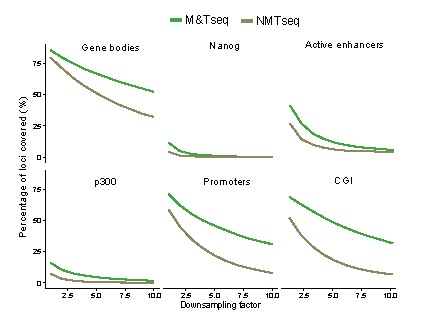
\includegraphics[width=0.8\linewidth]{scNMT_coverage2}
	\caption[]{\textbf{Comparison of the empirical coverage of DNA methylation with scM\&T-seq \cite{Angermueller2016}}.\\
	The y-axis displays the fraction of loci covered with at least 5 CpG sites. The x-axis displays the downsampling factor, where the value of 1 corresponds to no downsampling (i.e. the base line). To facilitate the comparison, we selected two cells that were sequenced at equivalent depth.}
	\label{fig:scnmt_coverage2}
\end{figure}

\subsubsection{Consistency with previous studies}

To assess the consistency with previous studies we quantified DNA methylation and chromatin accessibility using a running window throughout the genome. The resulting methylomes were compared to data sets from the same cell lines profiled with similar technologies, including scM\&T-seq\cite{Angermueller2016}, scBS-seq\cite{Smallwood2014} and bulk BS-seq\cite{Ficz2013}. We find that most of the variation is not attributed to the technology but to differences in culture condition (\Cref{scNMT_comparison}). This result is expected, as cells grown in 2i media remain in a native pluripotency state that is associated with genome-wide DNA hypomethylation \cite{Ficz2013}. Interestingly, the serum-cultured cells processed in this study overlapped with 2i-cultured cells from previous data sets. suggesting that they remained in a more pluripotent state. The most likely explanation for this variation is the differences in the cell lines (we used female EL16 versus male E14 in \cite{Angermueller2016,Smallwood2014,Ficz2013}). Previous studies have shown that female ESCs tend to show lower levels of mean global methylation, which is consistent with a more pluripotent phenotype \cite{Zvetkova2005}.\\

In terms of accessibility, no NOMe-seq measurements were available for ESCs at the time of the study, so we compared it to bulk DNase-seq data from the same cell type, yielding good consistency between datasets ($R=0.74$).
\begin{figure}[H]
	\centering
	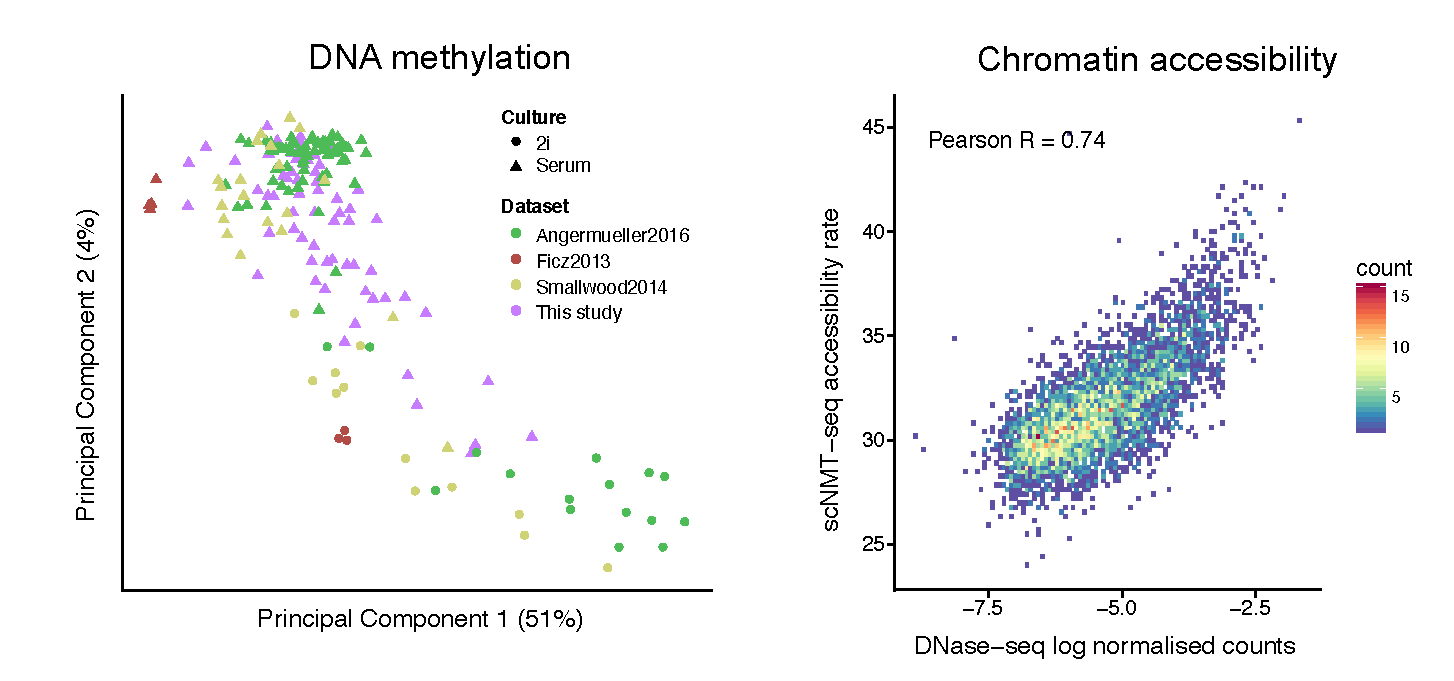
\includegraphics[width=1.0\linewidth]{scNMT_comparison}
	\caption[]{\textbf{Comparison of unsupervised genome-wide quantifications to published data sets}.\\
	(a) Principal Component Analysis of 1kb running windows. Missing values were imputed using the average methylation rate per locus.\\
	(b) Scatter plot of chromatin accessibility quantified over 10kb running windows of scNMT-seq data versus published bulk DNase-seq. For DNase-seq, accessibility is quantified as the log2 reads. The Pearson correlation was weighted by the GpC coverage in scNMT-seq data. }
	\label{fig:scnmt_comparison}
\end{figure}


\subsection{Quantification of DNA methylation and chromatin accessibility in known regulatory regions}

We pseudobulked the data across all cells and examined DNA methylation and chromatin accessibility levels at loci with known regulatory roles. We found that in CTCF binding sites and DNaseI hypersensitivity sites DNA methylation was decreased while chromatin accessibility was increased, as previously reported \cite{Pott2016}. As a control, we observe that cells which did not receive M.CviPI treatment showed globally low GpC methylation levels ( $\approx$ 2\%, \Cref{fig:scnmt_pseudobulk_profiles}).

\begin{figure}[H]
	\centering
	\includegraphics[width=0.7\linewidth]{scnmt_pseudobulk_profiles}
	\caption[]{\textbf{Accessibility and methylation profiles in regulatory genomic contexts.}\\
	First, we pseudobulk the data set by pooling information across all cells. Next, we compute running averages of the CpG methylation (red) and the GpC accessibility (blue) in consecutive non-overlapping 50bp windows. Solid line displays the mean across all genomic elements within a given annotation and the shading displays the corresponding standard deviation.\\
	(a) Profiles for scNMT-seq cells. (b) Profiles for scMT-seq cells
	}
	\label{fig:scnmt_pseudobulk_profiles}
\end{figure}

\subsection{Quantification of the association between molecular layers.}

We attempted to reconstruct the expected directional relationships between the transcriptome and the epigenome, namely the positive association between RNA expression and chromatin accessibility and the negative association between DNA methylation and RNA expression \cite{Thurman2012,Angermueller2016}.\\
To get a measure of the association (or coupling) between two molecular layers, we quantified a linear association per cell (across genes). Notice that this approach is not exclusive to single-cell data and can also be computed (more accurately) with bulk measurements. Reassuringly, this analysis confirmed, even within single cells, the expected positive correlation between chromatin accessibility and RNA expression, and the negative correlations between RNA expression and DNA methylation, and between DNA methylation and chromatin accessibility.

\begin{figure}[H]
	\centering
	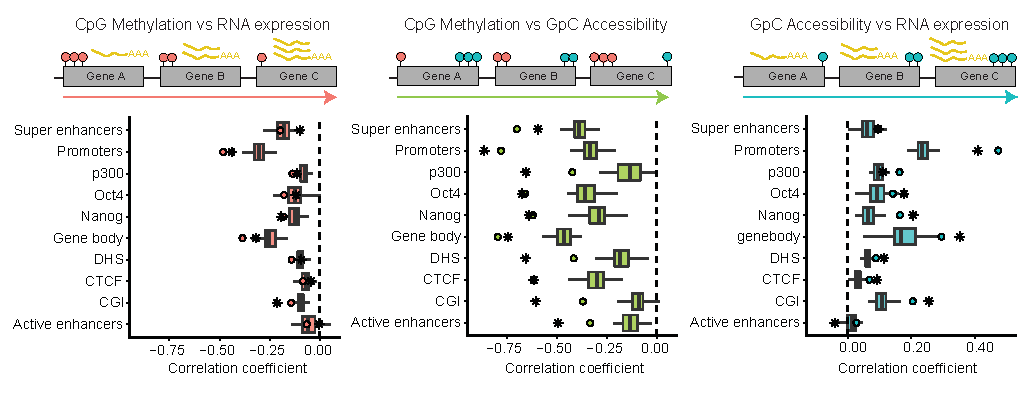
\includegraphics[width=1.0\linewidth]{scNMT_correlations_acrossgenes}
	\caption[]{\textbf{Quantification of linear associations between molecular layers.}\\
	The top diagram illustrates the computation of an association test per cell (across all loci in a given genomic context). The left panel shows DNA methylation versus RNA expression. The middle panel shows DNA methylation versus chromatin accessibility. The right panel shows RNA expression versus chromatin accessibility. The x-axis displays the Pearson correlation coefficients between two molecular layers, per genomic context (y-axis). The box plots summarise the distribution of correlation coefficients across cells. The dots and stars show the linear associations quantified in pseudo-bulked scNMT-seq data and published bulk data from the same cell types \cite{Ficz2013,ENCODE2012}, respectively. }
	\label{fig:scNMT_correlations_acrossgenes}
\end{figure}

% Consistently, when stratifiying the loci from \Cref{fig:scnmt_profiles} based on the expression level of the nearest gene, we observe that higher RNA expression is associated with chromatin openness and decreased DNA methylation levels \Cref{fig:scnmt_profiles_byexpr}. 
% \begin{figure}[H]
% 	\centering
% 	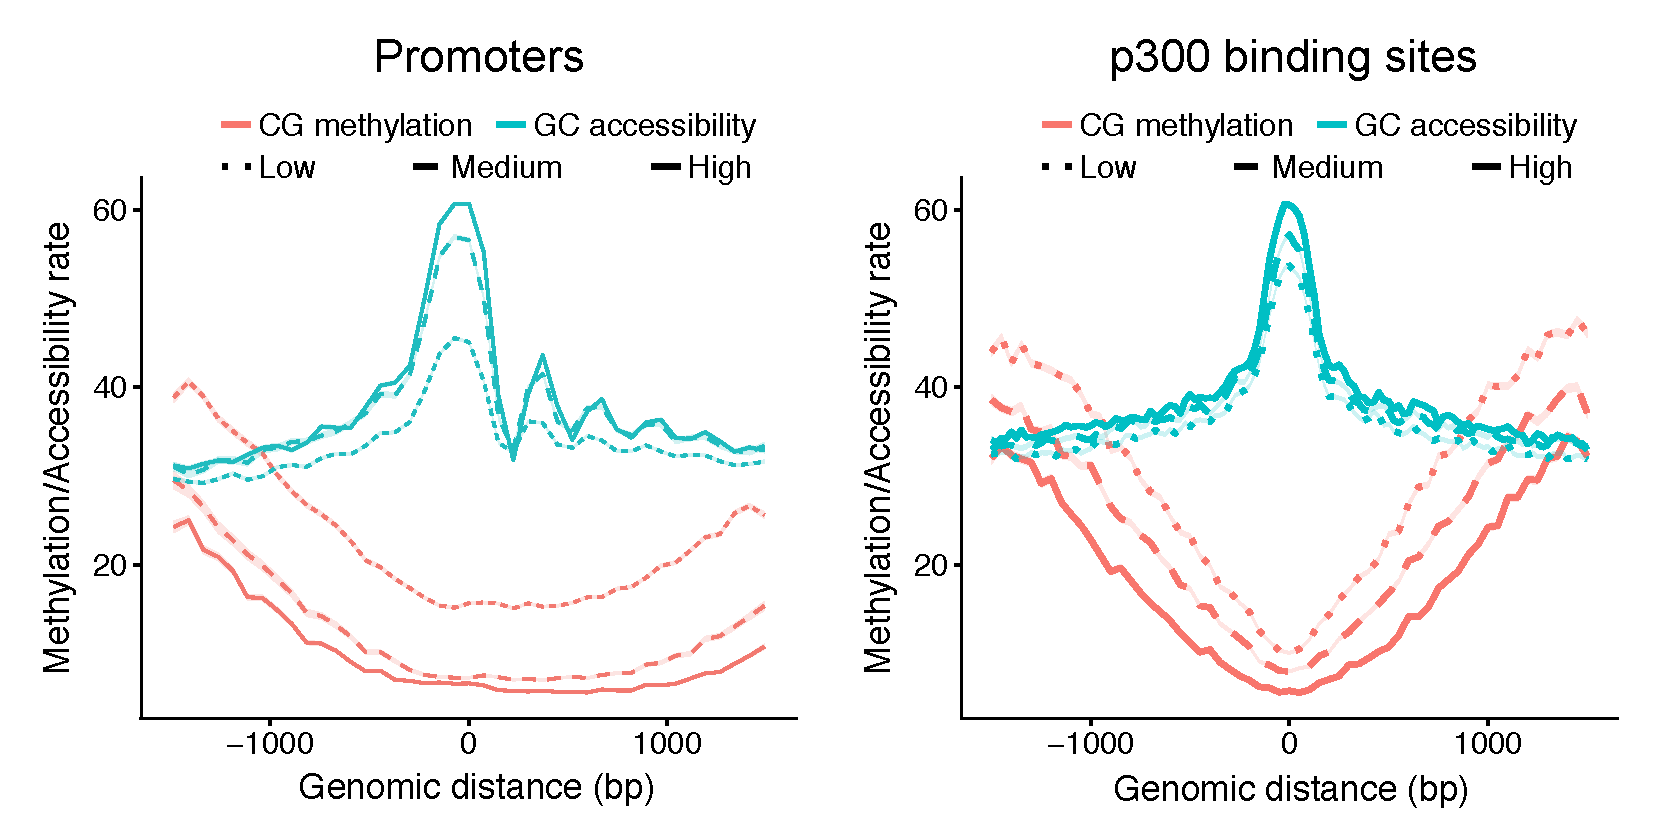
\includegraphics[width=0.9\linewidth]{scNMT_pseudobulk_profiles_byexpr}
% 	\caption[]{DNA methylation (red) and chromatin accessibility profiles (blue), stratified by RNA expression of the nearest gene. The profiles are quantified as in \Cref{fig:scnmt_profiles}. The RNA expression is discretised in three groups: log normalised counts less than 2 (low), between 2 and 6 (medium) and higher than 5 (high)}
% 	\label{fig:scnmt_profiles_byexpr}
% \end{figure}



\subsection{Identification of genomic elements with coordinated variability across molecular layers}

Having validated the quality of scNMT-seq data with a simple and relatively homogeneous data set, we next explored its potential to identify coordinated heterogeneity between the transcriptome and the epigenome.\\
We generated a second data set of 43 embryonic stem cells (after quality control), where we induced a differentiation process towards embryoid bodies by removing the LIF media for 3 days.\\Dimensionality reduction on the RNA expression data reveals the existence of two subpopulations: one with high expression of pluripotency markers (\textit{Esrrb} and \textit{Rex1}) and the other with high expression of differentiation markers (\textit{T} and \textit{Prtg}).

% \begin{figure}[H]
% 	\centering
% 	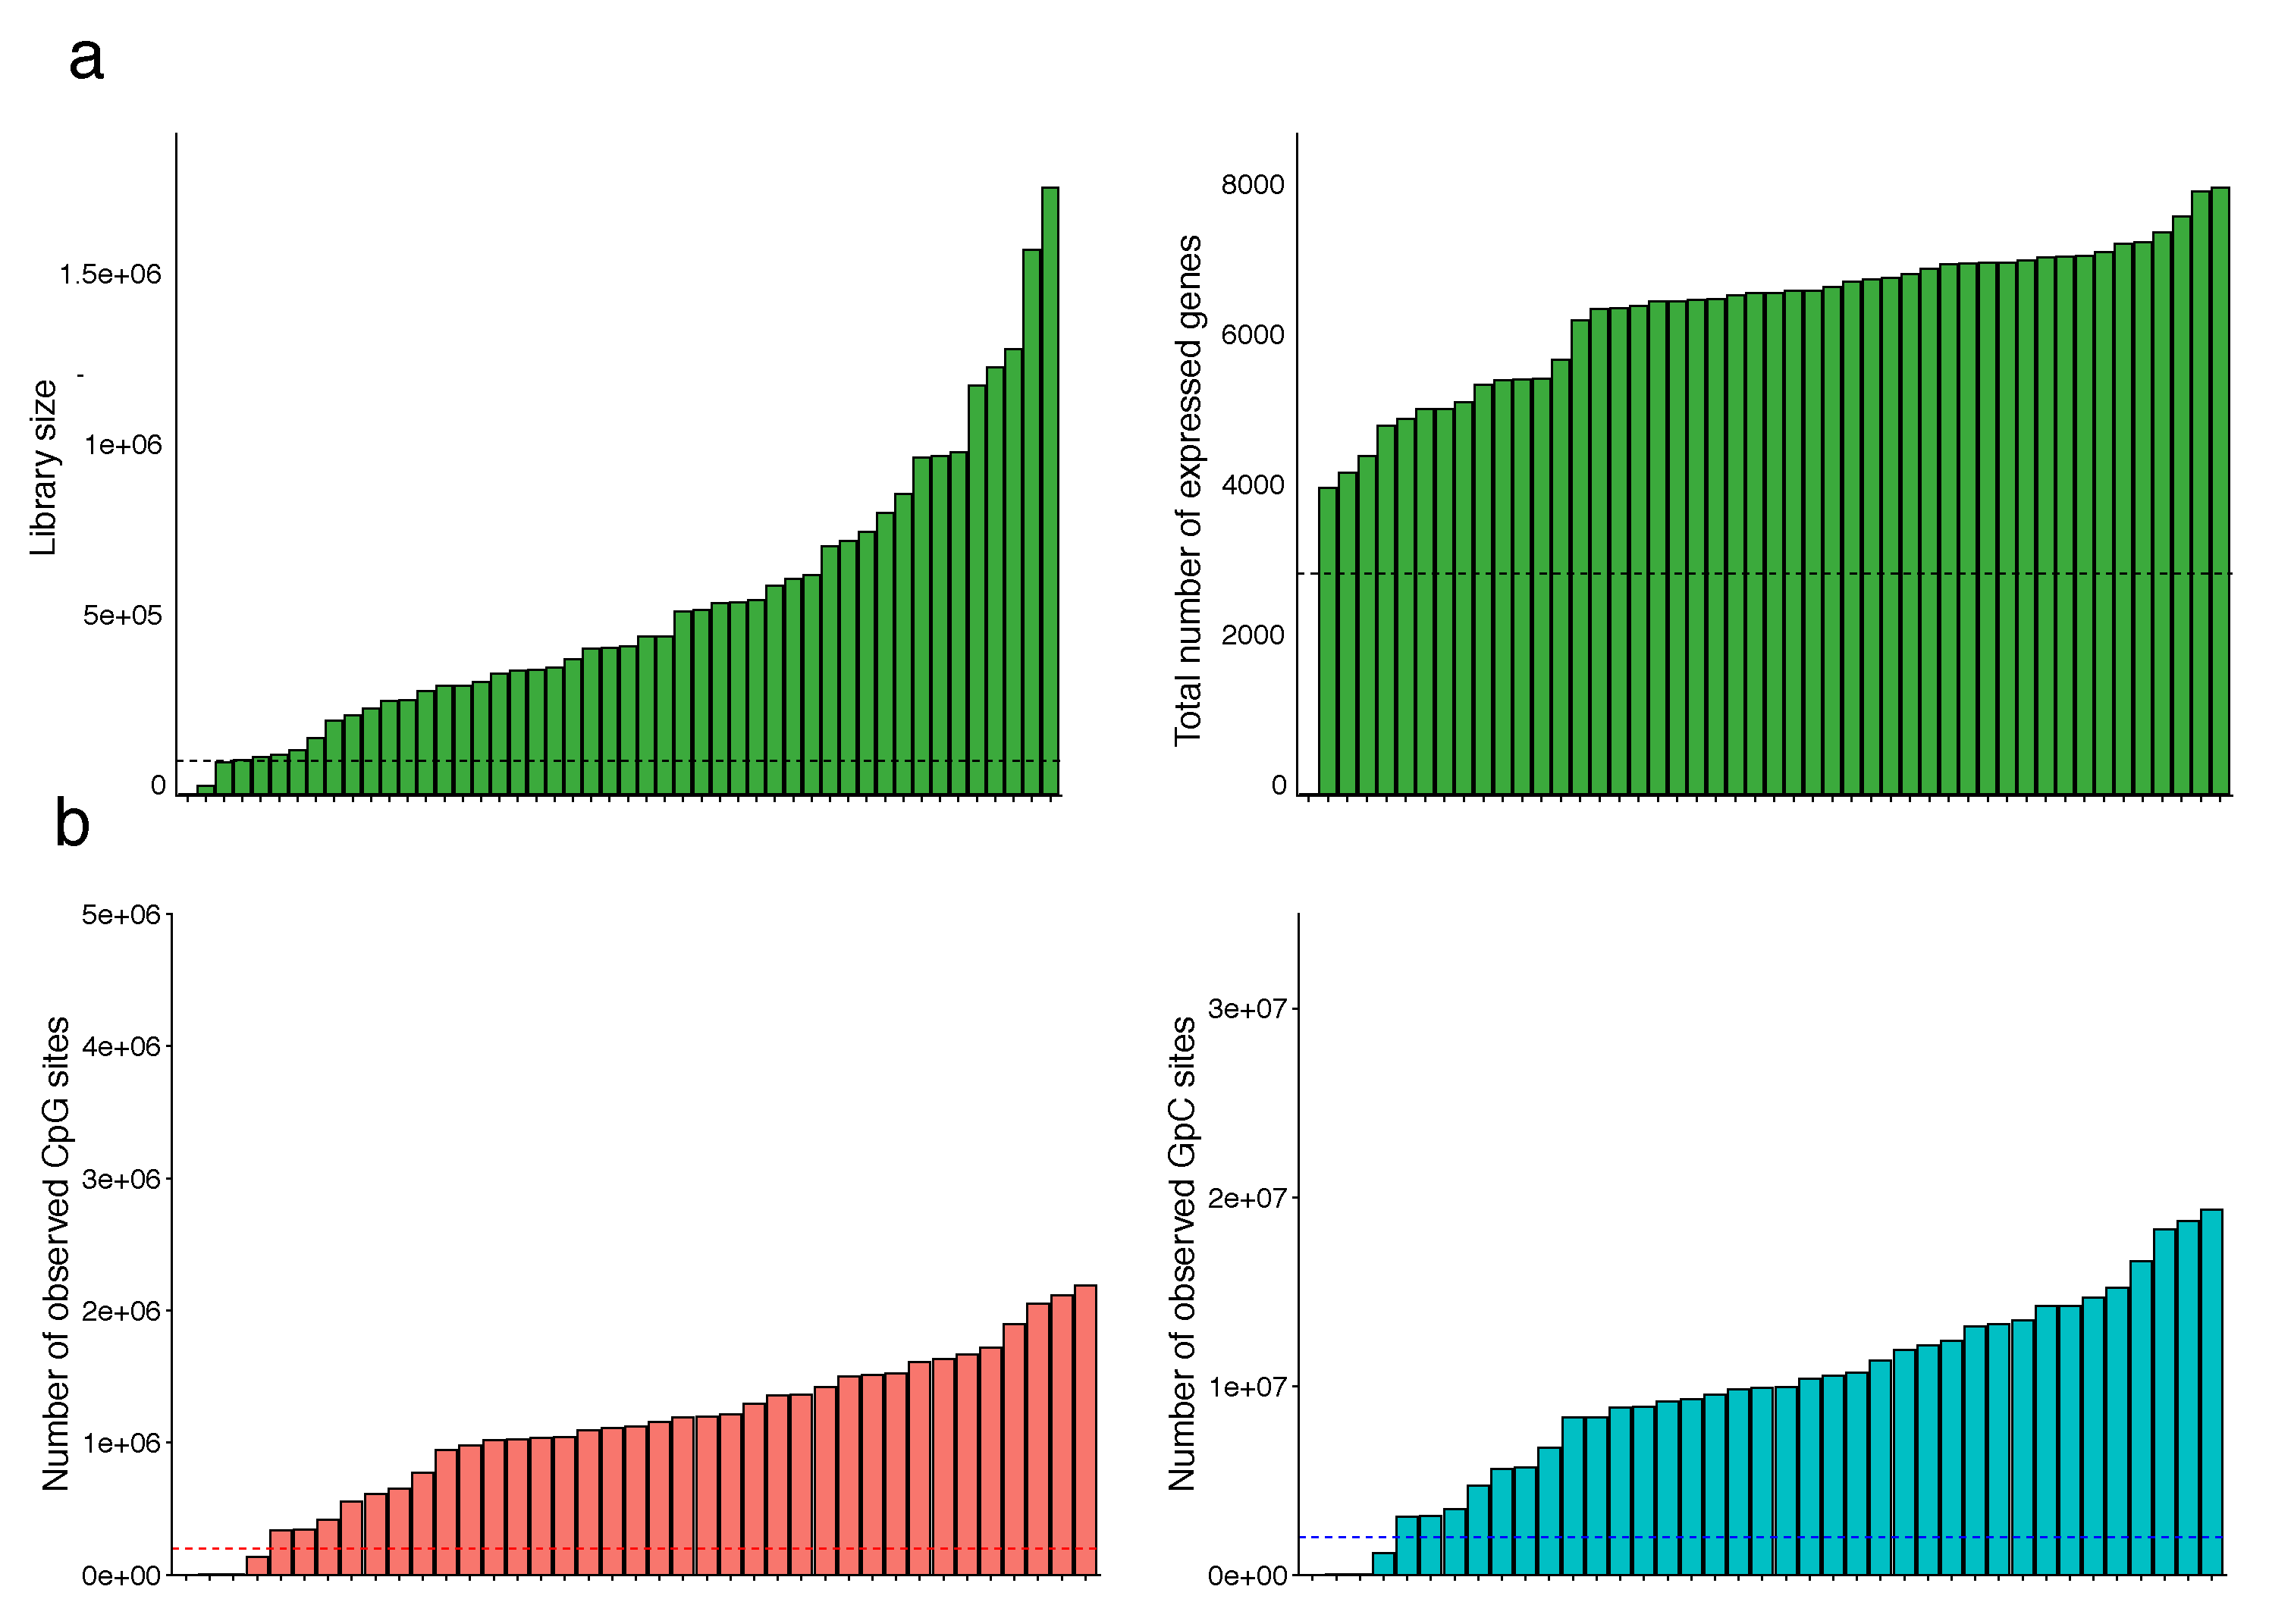
\includegraphics[width=0.8\linewidth]{scNMT_EB_QC}
% 	\caption[]{Quality control statistics on the 43 embryoid body cells. (a) number of aligned RNA reads per cell (left) and number of expressed genes (right). (b) Number of CpG sites (DNA methylation) observed. (c) Number of GpC sites (chromatin accessibility) observed. Dashed lines indicate binary thresholds, such that cells below the threshold are excluded for the downstream analysis.}
% 	\label{fig:scnmt_eb_qc}
% \end{figure}


\begin{figure}[H]
	\centering
	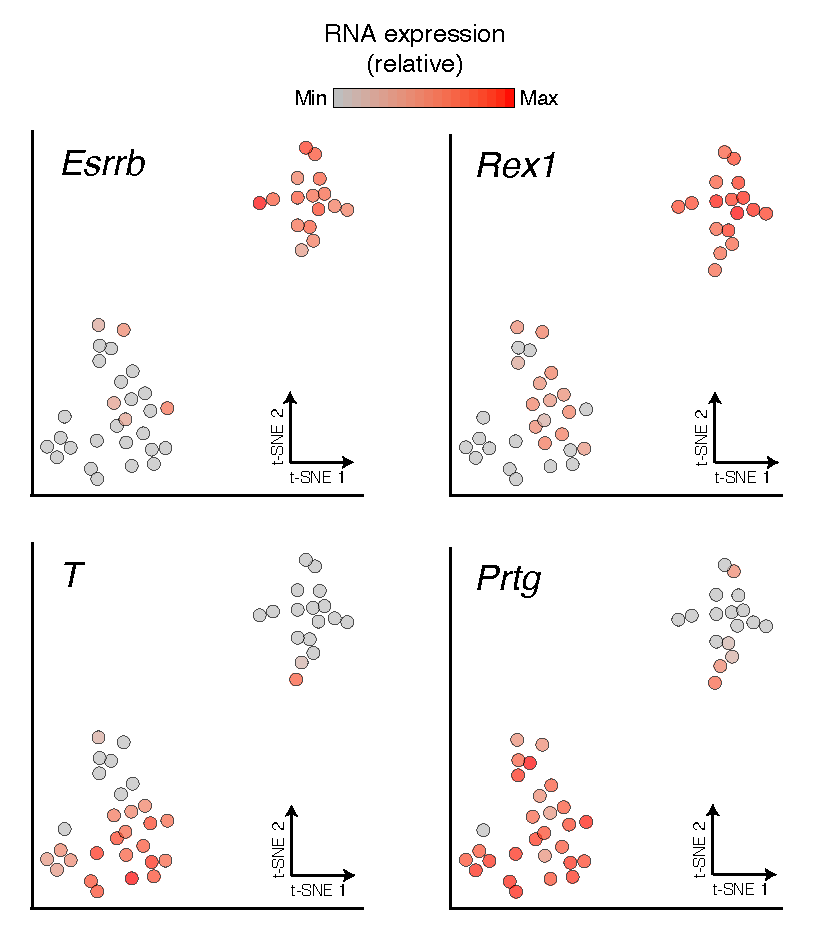
\includegraphics[width=0.65\linewidth]{scNMT_EB_RNA}
	\caption[]{\textbf{t-SNE representation of the RNA expression profiles for the embryoid body cells}.\\
	The scatter plots show a t-SNE representation of the EB data. Cells are coloured based on expression of pluripotency factors (top) and differentiation markers (bottom). }
	\label{fig:scnmt_eb_rna}
\end{figure}

Next, we tested for locus-specific associations between pairwise combinations of molecular layers (correlation across cells, \Cref{fig:scnmt_eb_correlations}).\\
First, considering correlations between DNA methylation and RNA expression, we identified a majority of negative associations, reflecting the known relationship between these two layers. In contrast, we obtained largely positive associations between chromatin accessibility and RNA expression, mainly in promoters, p300 binding sites and super enhancer regions. Finally, we found mostly negative associations between DNA methylation and chromatin accessibility. This confirms the expected direction of association between molecular layers, as reported in bulk studies.\\
As an illustrative example, we display the \textit{Esrrb} locus, a gene involved in early development and pluripotency \cite{Papp2012}. A previous study \cite{Angermueller2016}, identified a super enhancer near the gene that showed a high degree of correlation between DNA methylation and RNA expression changes. In our study, we find \textit{Esrrb} to be expressed primarily in the pluripotent cells, consistent with its role in early development. When examining the epigenetic dynamics of the corresponding super enhancers, we observe a strong negative correlation between DNA methylation and RNA expression, thus replicating previous findings. Additionally, we observe a strong negative relationship between DNA methylation and chromatin accessibility, indicating the two epigenetic layers are tightly coupled.

\begin{figure}[H]
	\centering
	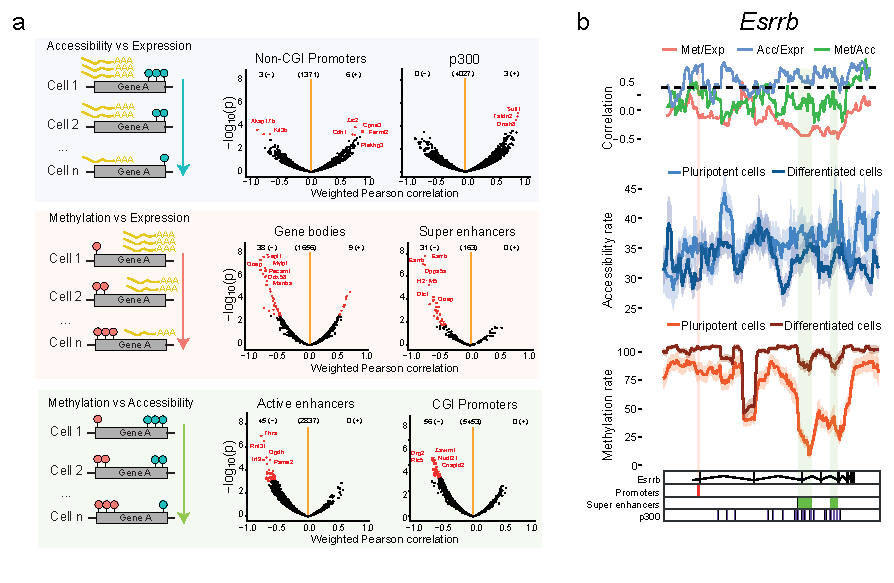
\includegraphics[width=1.0\linewidth]{scNMT_EB_correlations}
	\caption[]{
	\textbf{scNMT-seq enables the discovery of novel associations between transcriptomics and epigenetics at individual loci.}\\ 
	(a) Illustration for the correlation analysis, which results in one association test per locus (across cells). \\
	(b) Pearson correlation coefficient (x-axis) and log10 p-value (y-axis) from association tests between different molecular layers, stratified by genomic contexts. Significant associations (FDR<0.1), are highlighted in red.\\
	(c) Zoom-in view of the \textit{Esrrb} gene locus. Shown from top to bottom are: Pearson correlation between each pair of molecular layers. Accessibility (blue) and methylation (red) profiles shown separately for pluripotent and differentiated sub-populations; mean rates (solid line) and standard deviation (shade) were calculated using a running window of 10kb with a step size of 1kb. Track with genomic annotations highlighting the position of regulatory elements.
	}
	\label{fig:scnmt_eb_correlations}
\end{figure}


% \subsection{Inference of non-linear chromatin accessibility profiles at single nucleotide resolution}

% A clear advantage of scNMT-seq is the high resolution of the chromatin accessibility readouts, namely a binary output for each observed GpC dinucleotide. As illustrated in \Cref{fig:scnmt_pseudobulk_profiles}, GpC accessibility measurements rate extremely dynamic and display complex oscillatory patterns, likely due to presence of nucleosomes. This makes our approach of quantifying rates over a fixed genomic window not appropriate to capture the complexity of accessibility data. Therefore, we next attempted to exploit this high-resolution information to infer non-linear chromatin accessibility profiles at individual promoters.\\
% The approach we followed is based on BPRMeth \cite{Kapourani2018}, a generalized linear regression model with Gaussian basis functions, coupled with a Bernoulli likelihood. A model was fit for every gene and every cell, provided enough coverage (at least 10 GpC sites observed per gene across 40\% of cells). Examples of inferred regression patterns are shown below:

% \begin{figure}[H]
% 	\centering
% 	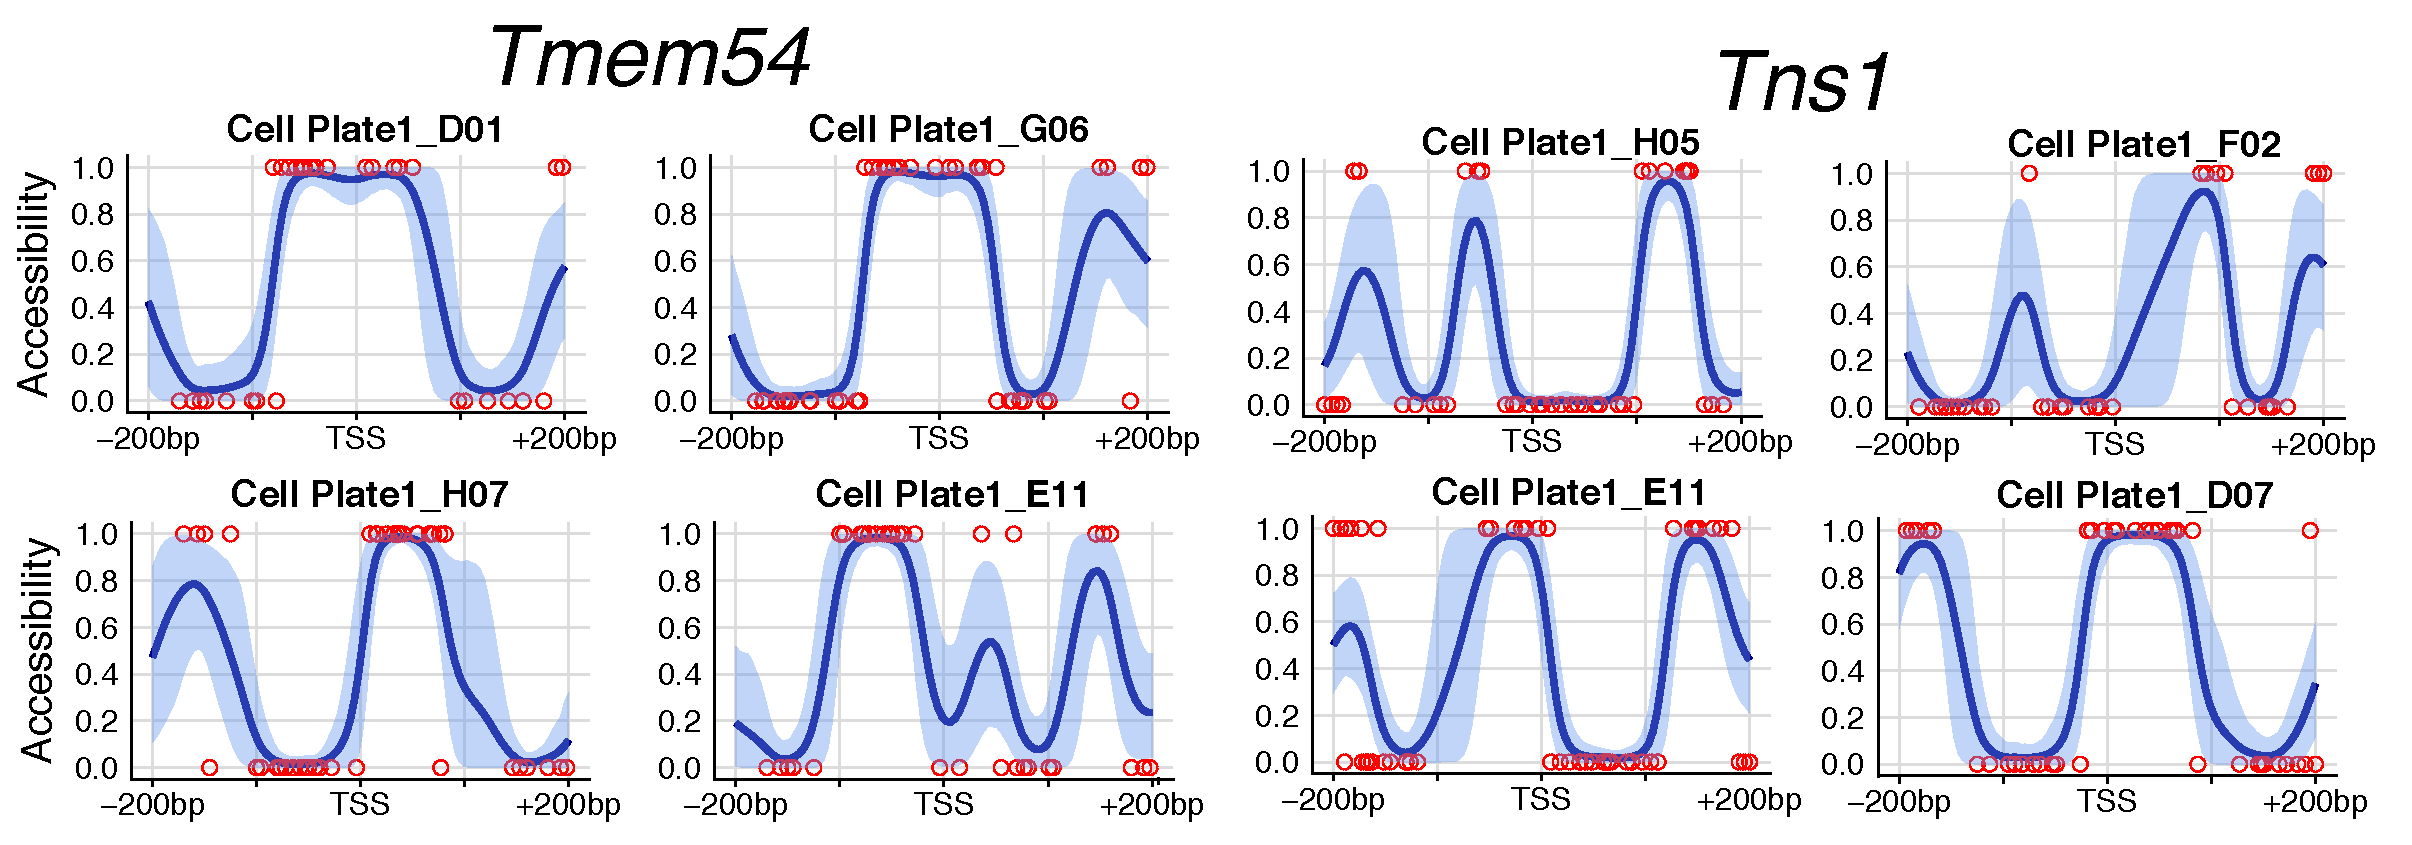
\includegraphics[width=0.9\linewidth]{scNMT_profiles_examples}
% 	\caption[]{\textbf{Illustrative examples of single-cell accessibility profiles around the transcription start site}.\\
% 	Shown are representative profiles for two genes, \textit{Tmem54} and \textit{Tns1}. Each panel corresponds to separate cell. The y-axis displays the binary GpC accessibility values, with 1 being accessibility and 0 inaccessible. The x-axis displays the genomic region around the TSS (200bp upstream and downstream). The blue area depicts the inferred (non-linear) accessibility profile using the BPRMeth model \cite{Kapourani2018}.}
% 	\label{fig:scnmt_profiles_examples}
% \end{figure}

% As a simple validation, we verified that highly expressed genes show characteristic patterns of nucleosome depleted regions around the TSS, whereas lowly expressed genes show low levels of chromatin accessibility:

% \begin{figure}[H]
% 	\centering
% 	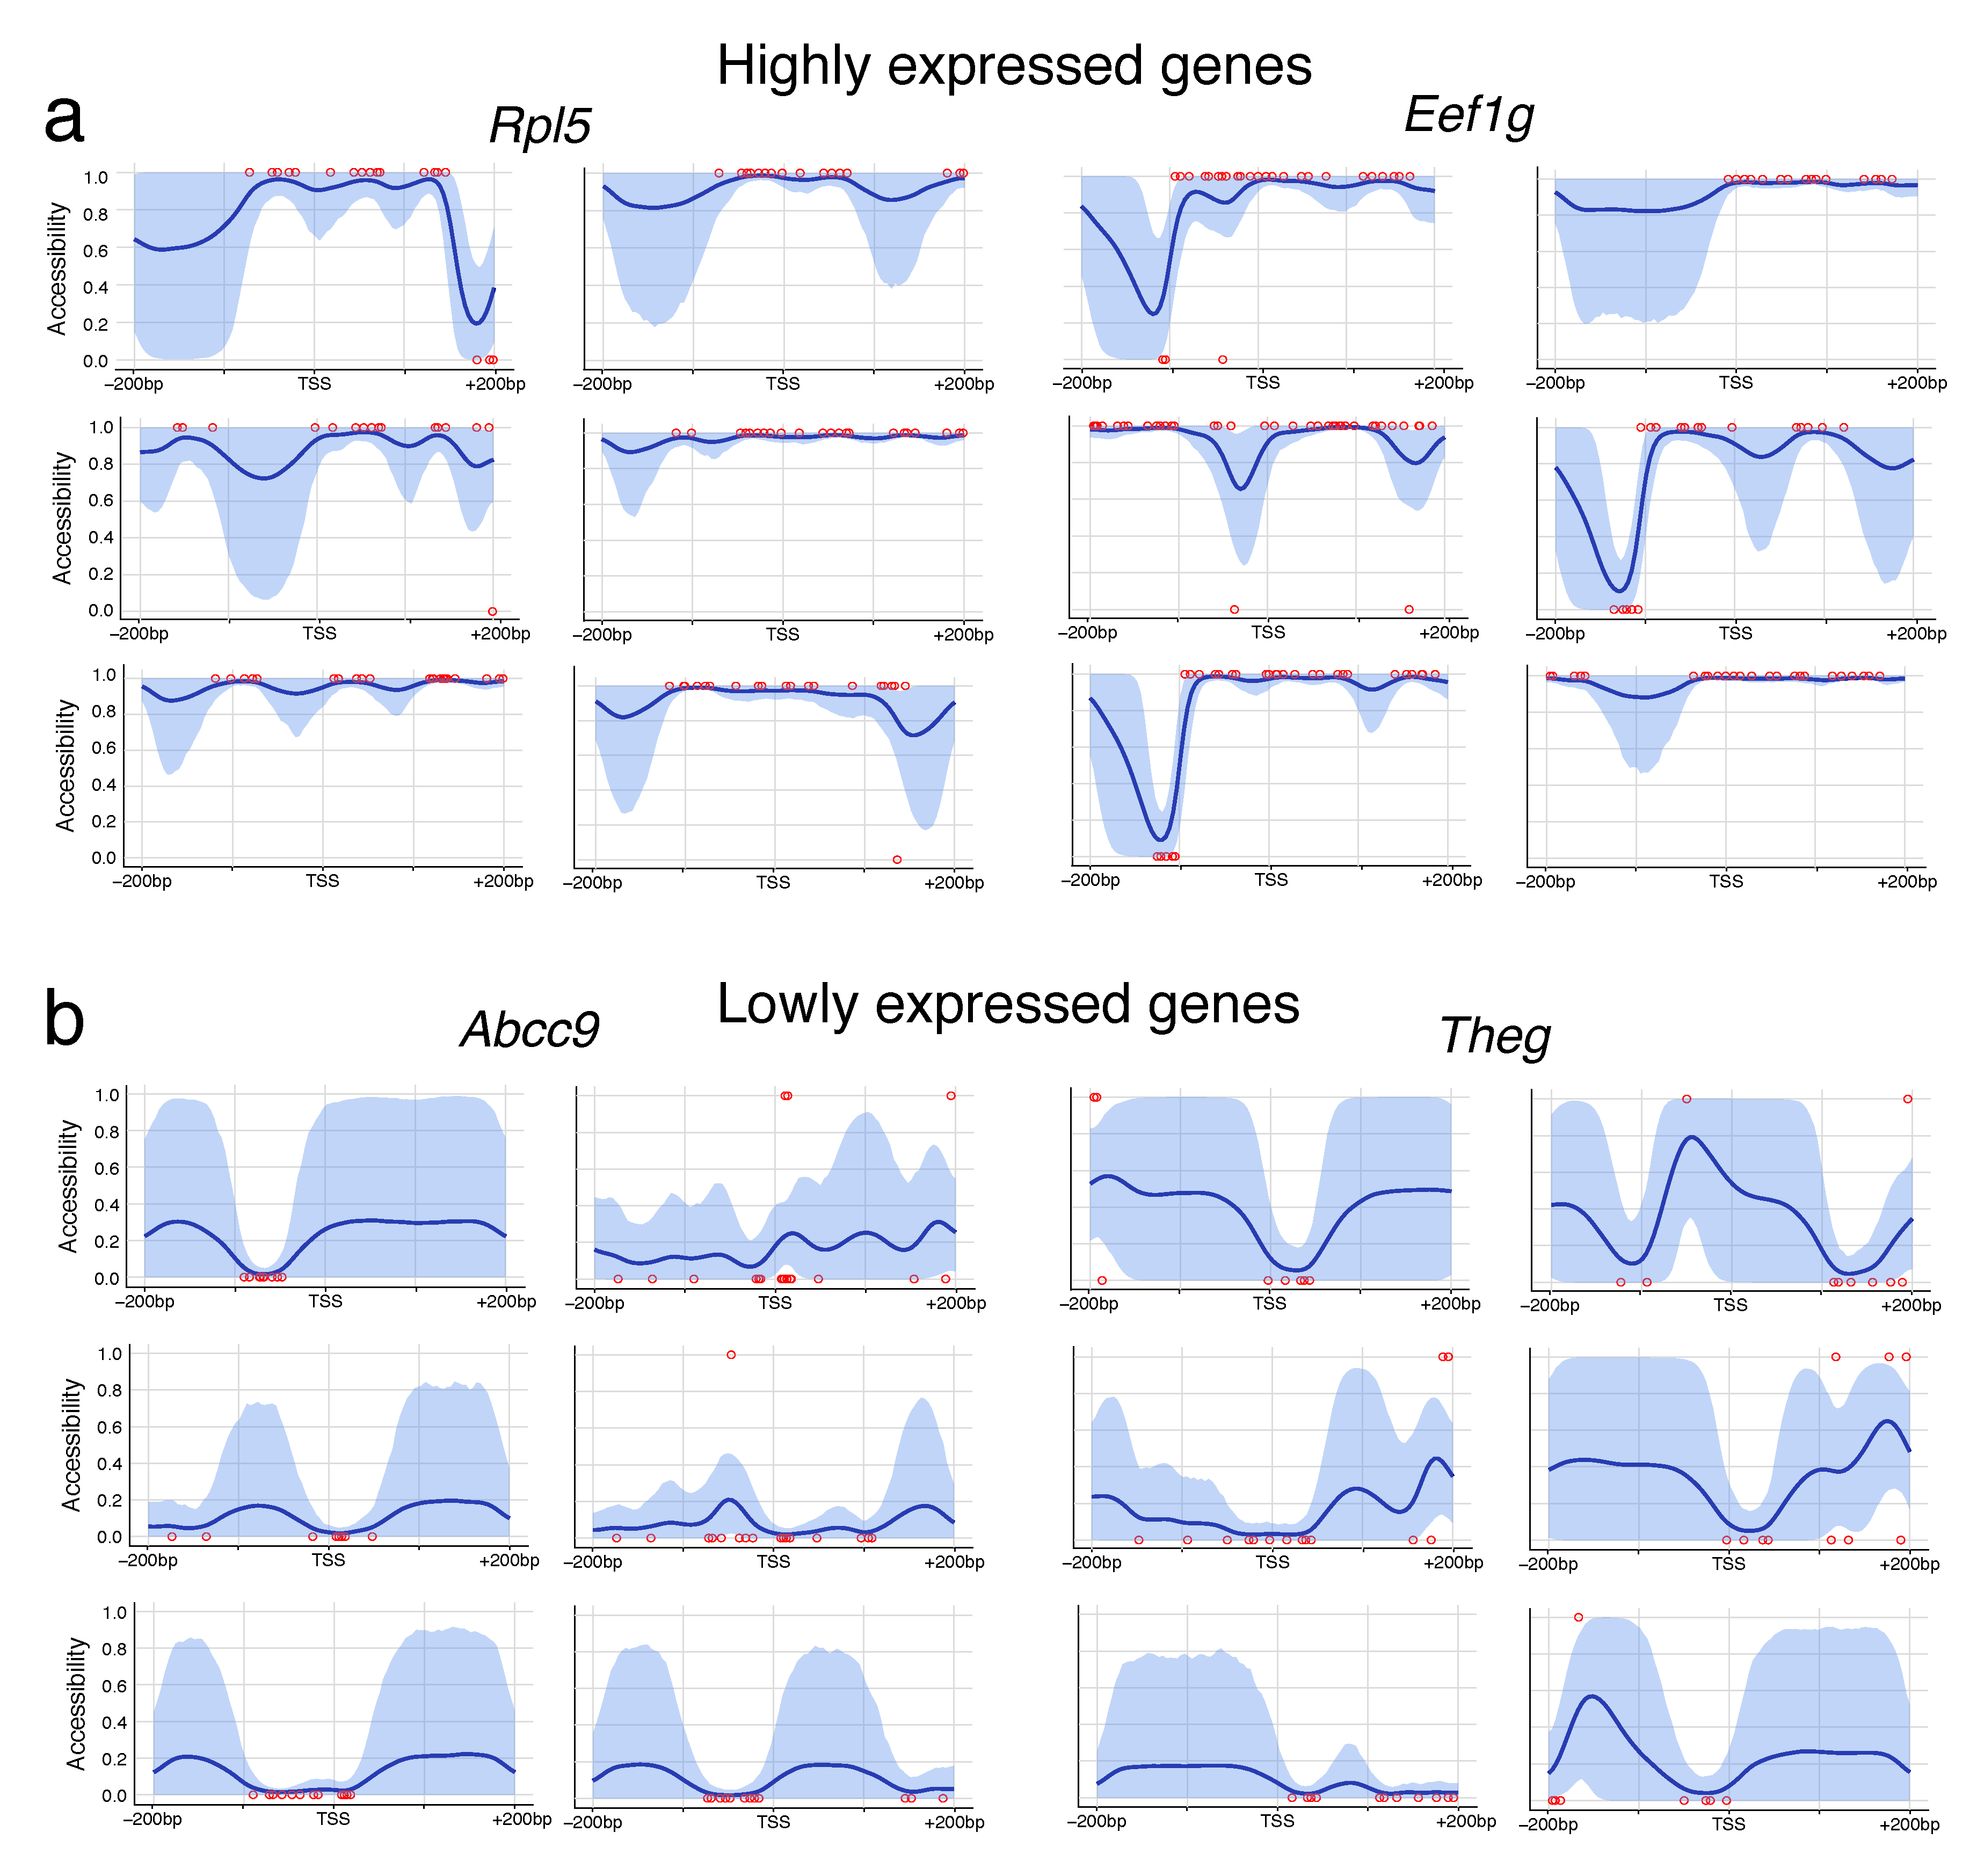
\includegraphics[width=0.9\linewidth]{scNMT_profiles_expr}
% 	\caption[]{\textbf{Single-cell accessibility profiles of representative genes with high and low expression levels.}\\
% 	Shown are \textit{Rpl5} and \textit{Eef1g} (high expression levels, top); \textit{Abcc9} and \textit{Theg} (low expression levels, bottom). Each panel corresponds to a separate cell. Axis are the same as in \Cref{fig:scnmt_profiles_examples}. }
% 	\label{fig:scnmt_profiles_highexpr}
% \end{figure}

% Using this statistical framework we attempted to link the heterogeneity in chromatin accessibility with the variability in RNA expression.\\
% A challenge of this computational representation is defining a unidimensional statistic that summarises the heterogeneity across cells (as the variance statistic in conventional rates), which can be in turn correlated with summary statistics from the RNA expression. The approach we followed here is to cluster cells (per gene) based on the similarity of the accessibility profiles, using a finite mixture model with an expectation-maximisation algorithm. The optimal number of clusters was estimated using a Bayesian Information Criterion.\\
% After model fitting, we considered the number of clusters as a proxy for accessibility heterogeneity, the rationale being that homogeneous genes will be grouped in a single cluster, while heterogeneous genes will contain a higher number of clusters. The result of the analysis is shown below:\\

% \begin{figure}[H]
% 	\centering
% 	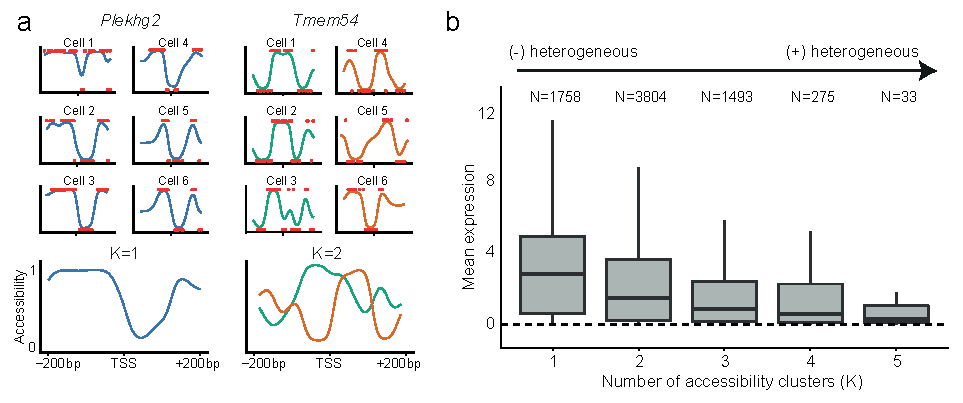
\includegraphics[width=0.9\linewidth]{scNMT_profiles_clusters}
% 	\caption[]{
% 	\textbf{Clustering chromatin accessibility profiles at gene promoters}. \\
% 	(a) Accessibility profiles are fitted for each cell and gene using 200 bp windows around the TSS. Then, a clustering step is applied for each gene and the most likely number of clusters is estimated using a Bayesian Information Criterion. Genes with higher numbers of clusters correspond to genes with increased heterogeneity compared to genes with small numbers of clusters.\\
% 	(b) Relationship between heterogeneity in the accessibility profile (x-axis) and average gene expression (across cells, y-axis).
% 	}
% 	\label{fig:scnmt_profiles_clusters}
% \end{figure}

% Genes with homogeneous accessibility profiles (fewer clusters) are associated with higher average expression levels. This includes genes with housekeeping functions, which are known to display highly conserved epigenetic features \cite{She2009}. In contrast, genes with heterogeneous accessibility (more clusters) are associated with lower expression levels. Interestingly, these genes are enriched for bivalent domains, containing both active H3K4me3 and repressive H3K27me3 histone marks (\Cref{fig:scnmt_profiles_histones}). As reported in previous studies, bivalent chromatin is normally associated with lowly-expressed genes that are poised for activation upon cell differentiation, thus playing a fundamental role in pluripotency and development \cite{Vastenhouw2012,Bernstein2006}

% \begin{figure}[H]
% 	\centering
% 	\includegraphics[width=0.80\linewidth]{scNMT_profiles_histones}
% 	\caption[]{\textbf{High levels of heterogeneity in chromatin accessibility are associated with the presence of bivalent histone marks (H3K4me3 and H3K27me3)}.\\
% 	Proportion of gene promoters marked with different sets of histone mark combinations (y-axis), stratified by number of accessibility clusters (x-axis)
% 	}
% 	\label{fig:scnmt_profiles_histones}
% \end{figure}


\subsection{Exploration of epigenome connections along a developmental trajectory}

The use of single-cell technologies has permitted the unbiased study of continuous trajectories by computationally reconstructing the \textit{pseudotemporal} dynamics from the molecular profiles \cite{Trapnell2014,Haghverdi2016,Saelens2018}. A novel opportunity unveiled by the introduction of single-cell multi-modal technologies is the study of epigenetic dynamics along trajectories inferred from the transcriptome. To explore this idea, we applied a diffusion-based pseudotime method\cite{Haghverdi2016} to the EB data set, using the RNA expression of the 500 genes with highest biological overdispersion\cite{Lun2016b}. The first diffusion component was used to reconstruct a pseudotemporal ordering of cells from pluripotent to differentiated states:

\begin{figure}[H]
	\centering
	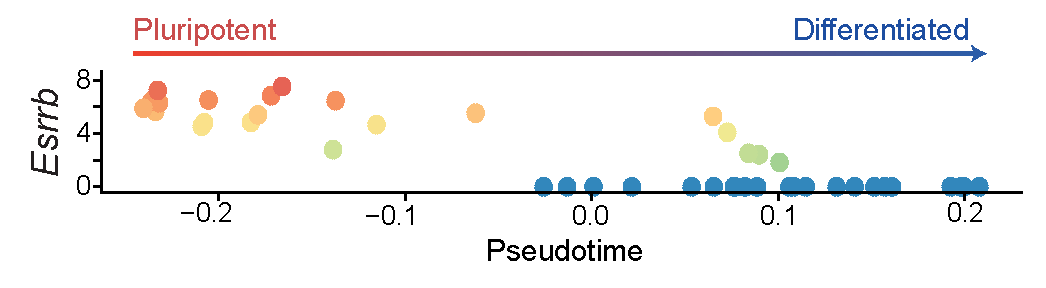
\includegraphics[width=0.75\linewidth]{scNMT_pseudotime}
	\caption[]{\textbf{Reconstruction of developmental trajectory in embryoid body cells from the RNA expression data}.\\
	Each dot corresponds to one cell. The y-axis displays expression of \textit{Esrrb}, a canonical pluripotency marker, and the x-axis shows the position of the cells in the first diffusion component.}
	\label{fig:scnmt_pseudotime}
\end{figure}


Using the pseudotime reconstruction we investigated whether the strength of association between molecular layers (as calculated in \Cref{fig:scNMT_correlations_acrossgenes}) are affected along the developmental trajectory. To do this, we correlated the correlation coefficient across genes between each pair of molecular layers (one value per cell) versus the pseudotime position (\Cref{fig:scnmt_pseudotime_coupling}). Importantly, this analysis is possible by the continuous nature of single-cell data and by the ability of scNMT-seq to profile three molecular layers at the same time.\\
We observe that for DNA methylation and chromatin accessibility, the negative correlation coefficients decreases in important regulatory genomic contexts (\Cref{fig:scnmt_pseudotime_coupling}), such that pluripotent cells have a notably weaker methylation-chromatin coupling than differentiated cells. This suggests that the strength of regulation between molecular layers can be altered during cell fate decisions.

\begin{figure}[H]
	\centering
	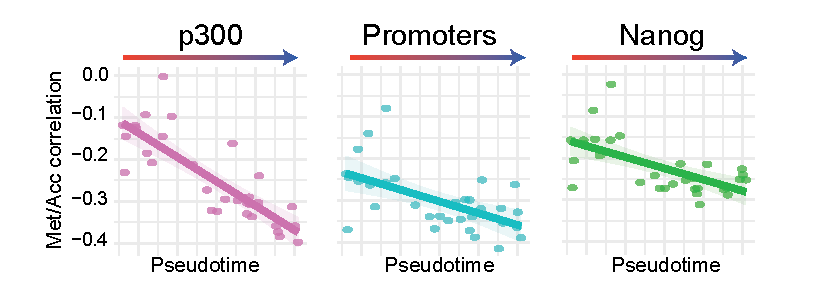
\includegraphics[width=0.9\linewidth]{scNMT_pseudotime_coupling}
	\caption[]{\textbf{Developmental trajectory is associated changes in methylation-accessibility coupling.}\\
	Shown is the location of each cell in pseudotime (x-axis) and the corresponding Pearson correlation coefficients between methylation and accessibility (y-axis) in three different genomic contexts with regulatory roles.
	}
	\label{fig:scnmt_pseudotime_coupling}
\end{figure}

\section{Conclusions and open perspectives}

In this Chapter I have introduced single-cell nucleosome, methylation and transcriptome sequencing (scNMT-seq), an experimental protocol for the genome-wide profiling of RNA expression, DNA methylation and chromatin accessibility in single cells. This novel assay is an important step forward in the field of single-cell multi-modal sequencing. Yet, as with other protocols, the technology is still in a very early stage and numerous developments are expected to occur in the next years. Some lines of research that I believe are important to improve scNMT-seq are the following:

\begin{itemize}

	\item \textbf{Scalability}: scRNA-seq protocols are reaching the astonishing numbers of millions of cells per experiment. This contrasts with the limited cell numbers achieved in current multi-modal assays, including scNMT-seq \cite{Cao2019,Cao2018,Guo2017}. As in scRNA-seq, the maturation of multi-modal techniques will display a trade-off between sensitivity and scalability \cite{Chappell2018}. scNMT-seq already provides high-resolution measurements, thus effort should be placed on making the protocol more scalable, which can be achieved by a series of technical improvements. First, barcodes are currently added at the end of the protocol, which limits cell numbers to the size of the plate. As in droplet-based methods or combinatorial indexing methods, adding the barcodes at the start of the protocol would enable the simultaneous processing of multiple pools of samples \cite{Dey2015,Mulqueen2018}. Second, the physical separation of mRNA from genomic DNA is performed at the beginning of the protocol, one cell at a time. Given that it is a time-consuming and expensive process, this step should be performed after pooling \cite{Dey2015}. Finally, albeit sequencing costs are decreasing \cite{Svensson2018}, the sequencing of scNMT-seq libraries remains expensive due to genome-wide coverage. Hence, I anticipate that efforts to decrease the library size by a pre-selection of the genetic material will be indispensable. Examples of such strategies are the digestion by restriction enzymes as in RRBS \cite{Guo2013}, an initial round of ATAC protocol to select open chromatin \cite{Spektor2018} or the pull-down of specific genomic regions using capture probes.

	\item \textbf{Imputation of missing epigenetic data}: because of the low amounts of starting material, single-cell methylation protocols are limited by incomplete CpG coverage \cite{Angermueller2017}. This becomes even more pronounced in scNMT-seq where almost $\approx$ 50\% of CpG dinucleotides are removed to avoid technical biases (see \Cref{section:scnmt_coverage}). Nonetheless, as discussed in \Cref{section:scnmt_protocol}, an important advantage of bisulfite approaches is that missing data can be discriminated from inaccessible chromatin (unlike in scATAC-seq). Therefore, the imputation of DNA methylation data will likely be a critical step to enable genome-wide analysis. Most of the imputation methods developed for bulk data are unsuccesful because they do not account for cell-to-cell variability \cite{Angermueller2017}. A successful single-cell strategy based on deep learning has been proposed (DeepCpG\cite{Angermueller2017}), but is a complex model that is difficult to train and does not scale to large data sets. Faster and accurate Bayesian approaches have also been considered (Melissa \cite{Kapourani2018b}), albeit the model is restricted to a small feature set and cannot perform genome-wide imputation.

	\item \textbf{Adding more molecular layers}: scNMT-seq can be adapted both experimentally and computationally to profile additional molecular layers. From the computational side, one could exploit the sequence information in the libraries to infer copy number variation or single nucleotide variants \cite{Poirion2018,Fan2018,McCarthy2018,Enge2017}. This approach has been successful at delineating the clonal substructure of somatic tissues and at tracking mutational signatures in cancer tissues. In addition, the full length transcript information enables the quantification of splice variants\cite{Huang2017}, allele-specific fractions\cite{Deng2014} and RNA velocity information \cite{LaManno2018}.\\
	From the experimental side, scNMT-seq could be combined with novel single-cell assays that quantify protein expression \cite{Stoeckius2017}, transcription factor binding \cite{Moudgil2019} and histone modifications \cite{Kaya-Okur2019}.

	% \item \textbf{Denoising}: in scNMT-seq the CGC positions (27\%) suffer from off-target effects of the GpC methylase \cite{Kelly2012}. In this work we have excluded those measurements to avoid undesired technical variation. Yet, no attempts have been carried to quantify this effect. If small enough, one could denoise the resulting CpG measurements by machine learning techniques that use sequence context information.
	% %The readouts from bisulfite sequencing are very sensitive \cite{XX}. 

	\item \textbf{Long reads}: the scNMT-seq libraries that were generated for this study contained short reads (75bp) that do not provide sufficient information about the regional context of the individual DNA molecule. By sequencing NOMe-seq libraries with long-read nanopore sequencing technology \cite{Lee2018} showed that one can obtain phased methylation and chromatin accessibility measurements and structural changes from a single assay. This approach could potentially unveil a more comprehensive understanding of the epigenome dynamics and its regulatory role on RNA expression.

\end{itemize}


% In conclusion, we have shown that the use of non-linear methods for summarising NOMe-seq accessibility data can yield novel insights into the chromatin organisation, nucleosome positioning and the consequent regulation of gene expression. Yet, we acknowledge that this novel computational methodology needs to be further validated using other data sets, and some improvements need to be implemented in order to ensure that robust biological signal can be extracted from single-cell studies. First, the use of faster inference frameworks, which has been implemented in the new version of the software \cite{Kapourani2018}. Second, the method requires a large number of measurements for an accurate regression. In this study we used relatively lenient thresholds and only $\approx$25\% genes passed coverage filtering. An attempt to improve this could be the use of Bayesian methods that simultaneously cluster and fit the regression model, effectively leveraging information about the similarity between individual cells \cite{Kapourani2018b}. Finally, one could aim at learning a joint model with DNA methylation and chromatin accessiblity to provide an extra layer of multi-modal information.



% Chapter 2
%\graphicspath{{Chapter2/Figs/}}

\chapter{Multi-Omics Factor Analysis (MOFA), a Bayesian model for integration of multi-omics data}

The work described in this chapter results from a collaboration with Wolfgang Huber's group at the EMBL (Heidelberg, Germany). It has been peer-reviewed and published in \cite{Argelaguet2018}.\\
The method was conceived by Florian Buettner, Oliver Stegle and me. I performed most of the mathematical derivations and implementation, but with significant contributions from Damien Arnol and Britta Velten. The CLL data application was led by Britta Velten whereas the single-cell application was led by me, but with joint contributions in either cases. Florian Buettner, Wolfgang Huber and Oliver Stegle supervised the project.\\
The article was jointly written by Britta Velten and me, with contributions from all authors.

\section{Theoretical foundations}

\subsection{Mathematical notation} \label{section:mathematical_notation}

\begin{itemize}[noitemsep]
	\item[--] Matrices are denoted with bold capital letters: $\bfW$
	\item[--] Vectors are denoted with bold non-capital letters: $\bfw$. If the vector comes from a matrix, we will use a single index to indicate the row that it comes from. If two indices are used, the first one corresponds to the row and the second one to the column. The symbol '$:$' denotes the entire row/column. For instance, $\bfw_{i}$ refers to the $i$th row from the $\bfW$ matrix, whereas $\bfw_{:,j}$ refers to the $j$th column.
	\item[--] Scalars are denoted with non-bold and non-capital letters: $w$. If the scalar comes from a 1-dimensional array (a vector), a single subscript will indicate its position in the vector. If the scalar comes from a 2-dimensional array, two indices will be shown at the bottom: the first one corresponding to the row and the second one to the column. For instance, $w_{i,j}$ refers to the value from the $i$th row and the $j$th column of the matrix $\bfW$, and $w_i$ to the $i$th value of the vector $\bfw$. In some cases, higher dimensional arrays (tensors) are used, and the use of multiple indices follows the same rationale.
	\item[--] $\boldzero_k$ is a zero vector of length $k$.
	\item[--] $\I_k$ is the identity matrix with rank $k$.
	\item[--] $\E_q[x]$ denotes the expectation of $x$ under the distribution $q$. When the expectations are taken with respect to the same distribution many times, we will avoid cluttered notation and we will instead use $\la x \ra$.
	\item[--] $\Ndist{x}{\mu,\sigma}$: $x$ follows a univariate normal distribution with mean $\mu$ and variance $\sigma$.
	\item[--] $\Gdist{x}{a,b}$: $x$ follows a gamma distribution with shape and rate parameters $a$ and $b$.
	\item[--] $\Bdist{x}{a, b}$: $x$ follows a beta distribution with shape and rate parameters $a$ and $b$.
	\item[--] $\text{Ber}(x|\theta)$: $x$ follows a Bernoulli distribution with parameter $\theta$.
	\item[--] $\mathds{1}_0$: Dirac delta function centered at 0.
	\item[--] $Tr(\bfX)$: Trace of the matrix \bfX
\end{itemize}

\subsection{Graphical notation for probabilistic models}

Probabilistic models can be represented in a diagrammatic format (i.e. a graph or a network) that offers a compact visual representation of complicated systems of probability distributions \cite{Bishop2006}. In a graphical model the relationship between the nodes becomes more explicit, namely their conditional independence properties which allow the joint distribution over all variables to be factorised into a series of simpler products involving subsets of variables \cite{Bishop2006}. The basic unit of a network is the node, which represents the different types of variables, including observed variables, unobserved probabilistic variables and unobserved parameters. The nodes are connected by unidirectional edges (arrows) which capture the conditional independence relationship between the variables.

For this thesis we adapted the graphical notations from~\cite{Dietz2010-technical-report-graphs}:

\begin{center}
  \begin{tabular}{m{8cm} m{2cm}}
    Observed variables & \tikz{\node[obs](){$Y$}} \\
    Unobserved probabilistic variables & \tikz{\node[latent](){$\theta$}} \\
    Unobserved parameters & \tikz{\node[latent,double, double distance=1pt](){$\theta$}} \\
    Repetition of node $\theta_n$ for $n\in\llbracket 1;N \rrbracket$ & \tikz{\node[latent](theta){$\theta_n$}; \plate[] {plateN} {(theta)} {$N$};} \\
    Conditional dependency between nodes: $p(Y,\theta) = p(Y|\theta)p(\theta)$ & \tikz{%
            \node[latent]   (theta) {$\theta$};
            \node[obs, xshift=1.5cm] (Y) {$Y$};
            \edge{theta}{Y}}
  \end{tabular}
\end{center}
% For simplicity, fixed hyperparameters are not represented on the graphical model. Unobserved parameters are only represented when optimised together with the unobserved probabilistic variables.



\subsection{Probabilistic modelling} \label{section:probabilistic_modelling}

A scientific model is a simple theoretical representation of a complex natural phenomenon to allow the systematic study of its behaviour. The general idea is that if a model is able to explain some observations, it might be capturing its true underlying laws and can therefore be used to make future predictions.
In particular, statistical models are a powerful abstraction of nature. They consist on a set of observed variables and a set of (hidden) parameters. The procedure of fitting the parameters using a set of observations is called inference or learning.

One of the major challenges of inference when dealing with real data sets is the distinction between signal and noise. An ideal model should learn only the information relevant to gain explanatory power while disregarding the noise. However, this is a non-trivial task in most practical situations. Very complex models will tend to overfit the training data, capturing large amounts of noise and consequently leading to a bad generalisation performance to independent data sets. On the other hand, simplistic models will fit the data poorly, leading to poor explanatory power.

The ideas above can be formalised using the framework of probability and statistics.


\subsubsection{Maximum likelihood inference} \label{section:maximum_likelihood}

A common approach is to define a statistical model of the data $\bfY$ with a set of parameters $\btheta$ that define a probability distribution $p(\bfY|\btheta)$, called the likelihood function. A simple approach to fit a model is to estimate the parameters $\hat{\btheta}$ that maximise the likelihood:
\[
	\hat{\btheta} = \argmax_{\btheta} p(\bfY|\btheta)
\]
This process is called maximum likelihood learning\cite{Stigler2008,Bishop,Murphy}. However, in this setting there is no penalisation for model complexity, making maximum likelihood solutions prone to overfit in cases where the data is relatively sparse. Generalisations that account for model complexity have been proposed and include regularising terms that shrink parameters to small values. However, these are often particular cases of the more general framework of Bayesian statistics \cite{Hastie,Bishop,Murphy}.

\subsubsection{Bayesian inference}  \label{section:bayesian_inference}
In the Bayesian framework, the parameters themselves are treated as random unobserved variables and we aim to obtain probability distributions for $\btheta$, rather than a single point estimate. To do so, prior beliefs are introduced into the model by specifying a prior probability distribution $p(\btheta)$. Then, using Bayes' theorem \cite{Bayes1763}, the prior hypothesis is updated based on the observed data $\bfY$ by means of the likelihood $p(\bfY|\btheta)$ function, which yields a posterior distribution over the parameters:
\[
	p(\btheta|\bfY) = \frac{p(\bfY|\btheta) p(\btheta)}{p(\bfY)}
\]
where $p(\bfY)$ is a constant term called the marginal likelihood, or model evidence \cite{Bishop,Murphy}.\\
The choice of the prior distribution is a key part of Bayesian inference and captures beliefs about the distribution of a variable before the data is taken into account. With asymptotically large sample sizes, the choice of prior has negligible effects on the posterior estimates, but it becomes critical with sparse data \cite{Bishop,Murphy,Gelman2013}.

There are two common considerations when defining the prior distributions. The first relates to the incorporation of subjective information, or predefined assumptions, into the model. For example, one could adapt the prior distribution to match the results from previous experiments (i.e. an informative prior). Alternatively, if no information is available one could set set uninformative priors by following maximum entropy principles \cite{Jaynes1968}.

The second strategy is based on convenient mathematical properties to make inference tractable. If the likelihood and the prior distributions do not belong to the same family of probability distributions (they are not conjugate) then inference becomes more problematic \cite{Raiffa1961,Bishop,Murphy,Gelman2013}. The existence of conjugate priors is one of the major reasons that justify the widespread use of exponential family distributions in Bayesian models \cite{Gelman2013}. An example is the Automatic Relevance Determination prior discussed in \Cref{section:ard}.

Again, the milestone of Bayesian inference is that an entire posterior probability distribution is obtained for each unobserved variable. This has the clear advantage of naturally handling uncertainity in the estimation of parameters. For instance, when making predictions, a fully Bayesian approach attempts to integrate over all the possible values of all unobserved varaibles, effectively propagating uncertainity across multiple layers of the model. Nevertheless, this calculation is sometimes intractable and one has to resort to point estimates \cite{Bishop,Murphy,Gelman2013}. The simplest approximation to the posterior distribution is to use its mode, which leads to the maximum a posteriori (MAP) estimate:
\[
	\hat{\btheta} = \argmax_{\btheta} p(\btheta) p(\bfY|\btheta) 
\]
This is similar to the maximum likelihood objective function, but with the addition of a term $p(\btheta)$. When the prior dsitribution is chosen smartly, this term penalises for model complexity. Therefore, in contrast to standard (non-penalised) maximum likelihood inference, Bayesian approaches naturally handle the problem of model complexity and overfitting\cite{Bishop,Murphy,Gelman2013}. At the limit of infinite observations, the influence of the prior to the posterior is negligible and the MAP estimate converges towards the Maximum likelihood estimate, hence providing a rational link between the two inference frameworks.

\subsubsection{Deterministic approaches for Bayesian inference} \label{section:deterministic_bayesian_inference}
The central task in Bayesian inference is the direct evaluation of the posterior distributions and/or the computation of expectations with respect to the posterior distributions. In sufficiently complex models, closed-form solutions are not available and one has to resort to approximation schemes, which broadly fall into two classes: stochastic or deterministic \cite{Gelman2013,Blei2016}. 

Stochastic approaches hinge on the generation of samples from the posterior distribution via a Markov Chain Monte Carlo (MCMC) framework. Such techniques have the appealing property of generating exact results at the asymptotic limit of infinite computational resources. However, in practice, sampling approaches are computationally demanding and suffer from limited scalability to large data sets \cite{Blei2016}. \\
In contrast, deterministic approaches are based on analytical approximations to the posterior distribution, which often lead to biased results. Yet, given the appropriate settings, these approaches are potentially much faster and scalable to large applications \cite{Bishop,Murphy,Blei2016}.

\subsubsection{Laplace approximation} \label{section:laplace_approximation}
The Laplace approximation is probably the simplest of the deterministic tecniques, where the aim is to construct a Gaussian approximation around the mode of the true posterior distribution using a second-order Taylor expansion \cite{Bishop,Murphy}.\\
Suppose $\bfX$ contains all unobserved variables. The true posterior distribution can be written as:
\[
p(\bfX) = \frac{f(\bfX)}{Z}
\]
where $f(\bfX)$ is a function that depends on the unobserved variables and $Z$ is an unknown normalisation constant to ensure that $\int p(\bfX) d\bfX = 1$.

The second-order Taylor expansion of $\log f(\bfX)$ centered around its (known) mode $\hat{\bfX}$ is: 
\[
	\log f(\bfX) \approx \log f(\hat{\bfX}) - \frac{1}{2} (\bfX-\hat{\bfX})^T \bfA (\bfX-\hat{\bfX})
\]
where $\bfA = \nabla^2 \log f(\hat{\bfX})$ is the Hessian matrix of $\log f(\bfX)$ evaluated at $\hat{\bfX}$.\\
Notice three things. First, the first-order term of the Taylor expansion is zero because $\hat{\bfX}$ is a stationary point. Second, the $\log$ function is monotonically increasing and therefore a maximum of $\log f(\bfX)$ is also a maximum of $f(\bfX)$. Third, the mode of the posterior $p(\bfX)$ must be known, which requires the use of (complex) optimisation algorithms.\\
Taking the exponential in both sides:
\[
	f(\bfX) \approx f(\hat{\bfX}) \exp\{ -\frac{1}{2} (\bfX-\hat{\bfX})^T \bfA (\bfX-\hat{\bfX}) \}
\]
which leads to the following multivariate Gaussian distribution approximation $q(\bfX) = \Ndist{\bfX}{\hat{\bfX},\bfA}$:
\[
	q(\bfX) = \frac{\mid A \mid^{1/2}}{(2\pi^{d/2})} \exp\{ -\frac{1}{2} (\bfX-\hat{\bfX})^T \bfA (\bfX-\hat{\bfX}) \}
\]
where $d$ is the number of unobserved variables. \\
Despite its simplicity, the Laplace approximation is a useful strategy that has been successfully applied in practice. Nonetheless, this approximation has notable caveats: first, is limited by its own local definition, ignoring all the density beyond the mode of the posterior. Second, it does not apply to discrete variables. Third, the inversion of the Hessian is very expensive in high-dimensional settings.
	% More sophisticated generalisations of the Laplace approximation have also been proposed \cite{Rue2009}
	% To-do: check where does the inverse appear

\subsubsection{Variational inference}  \label{section:variational_inference}

Variational inference is a deterministic family of methods that have been receiving widespread attention due to a positive balance between accuracy, speed, and ease of use \cite{Blei2016, Zhang2017}. The core framework is derived below.

In variational inference the true (but intractable) posterior distribution $p(\bfX|\bfY)$ is approximated by a simpler (variational) distribution $q(\bfX|\bTheta)$ where $\bTheta$ are the corresponding parameters. The parameters, which we will omit from the notation, need to be tuned to obtain the closest approximation to the true posterior.\\
The distance between the true distribution and the variational distribution is calculated using the KL divergence:
\[
\KL(q(\bfX)||p(\bfX|\bfY)) = - \int_z q(\bfX) \log \frac{p(\bfX|\bfY)}{q(\bfX)}
\]
Note that the KL divergence is not a proper distance metric, as it is not symmetric. In fact, using the reverse KL divergence $\KL(q(\bfX)||p(\bfX|\bfY))$ defines a different inference framework called expectation propagation \cite{Minka2001}.

If we allow any possible choice of $q(\bfX)$, then the minimum of this function occurs when $q(\bfX)$ equals the true posterior distribution $p(\bfX|\bfY)$. Nevertheless, since the true posterior is intractable to compute, this does not lead to any simplification of the problem. Instead, it is necessary to consider a restricted family of distributions $q(\bfX)$ that are tractable to compute and subsequently seek the member of this family for which the KL divergence is minimised.

Doing some calculus it can be shown (see \cite{Bishop,Murphy}) that the KL divergence $\KL(q(\bfX)||p(\bfX|\bfY))$ is the difference between the log of the marginal probability of the observations $\log(\bfY)$ and a term $\Lagr(\bfX)$ that is typically called the Evidence Lower Bound (ELBO):
\[
	\KL(q(\bfX)||p(\bfX|\bfY)) = \log(\bfX) - \Lagr(\bfX)
\]
Hence, minimising the KL divergence is equivalent to maximising $\Lagr(\bfX)$ \Cref{fig:ELBO}:
\begin{align} \label{eq_elbo1} \begin{split}
	\Lagr(\bfX) &= \int q(\bfX) \Big( \log \frac{p(\bfX|\bfY)}{q(\bfX)} + \log p(\bfY) \Big) d\bfX \\
	%&= \int \Big( q(\bfX) \log \frac{p(\bfX|\bfY)}{q(\bfX)} + q(\bfX)\log p(\bfY) \Big) d\bfX\\
	%&= \E_q [\log p(\bfX|\bfY)] - \E_q [\log q(\bfX)] + \E_q [\log p(\bfY)] \\
	&= \E_q [\log p(\bfX,\bfY)] - \E_q [\log q(\bfX)]
\end{split} \end{align}
The first term is the expectation of the log joint probability distribution with respect to the variational distribution. The second term is the entropy of the variational distribution.
Importantly, given a simple parametric form of $q(\bfX)$, each of the terms in \Cref{eq_elbo1} can be computed in closed form.\\
In some occasions (see section X), we will use the following form for the ELBO:
\begin{equation} \label{eq_elbo2}
	\Lagr(\bfX) = \E_q [\log p(\bfY|\bfX)] + (\E_q [\log p(\bfX)] - \E_q [\log q(\bfX)])
\end{equation}
where the first term is the expectation of the log likelihood and the second term is the difference in the expectations of the $p$ and $q$ distributions of each hidden variable.

In conclusion, variational learning involves minimising the KL divergence between $q(\bfX)$ and $p(\bfX|\bfY)$ by instead maximising $\Lagr(\bfX)$ with respect to the distribution $q(\bfX)$. The following image summarises the general picture of variational learning:

\begin{figure}[H]
	\centering
	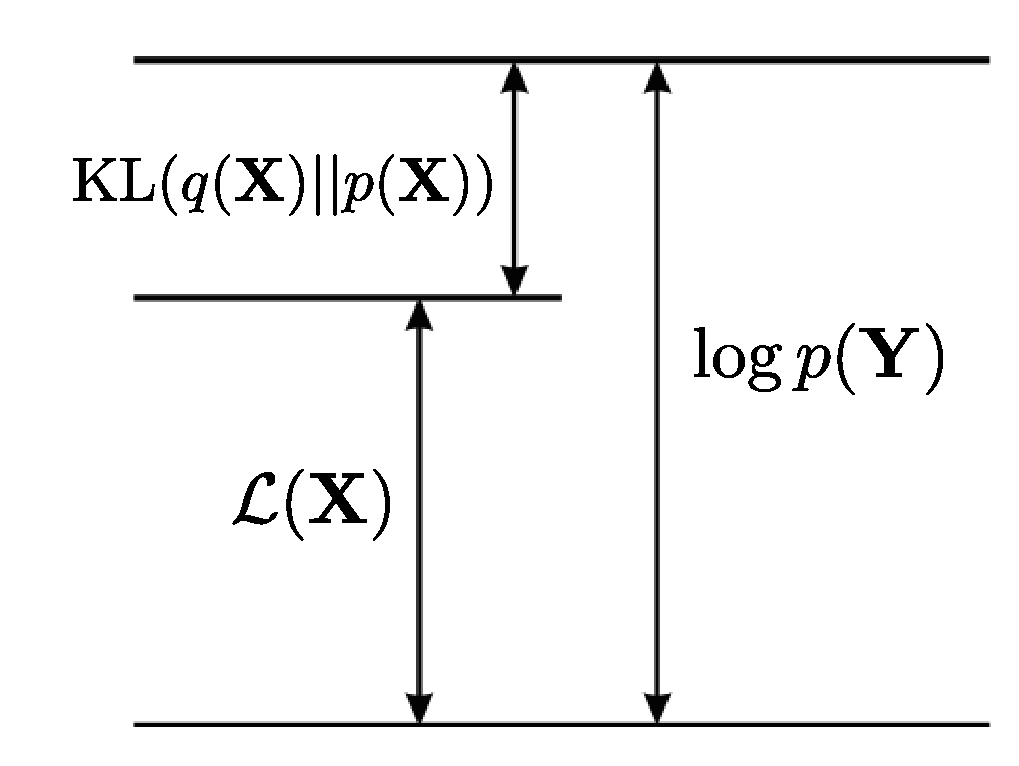
\includegraphics[width=0.35\linewidth]{lower_bound}
	\caption{The quantity $\Lagr(\bfX)$ provides a lower bound on the true log marginal likelihood $\log p(\bfY)$, with the difference being given by the Kullback-Leibler divergence $\KL(q||p)$ between the variational distribution $q(\bfX)$ and the true posterior $p(\bfX|\bfY)$}
	\label{fig:ELBO}
\end{figure}

There are several approaches to define $q(\bfX)$, the two most commonly used are called (unparametric) mean-field and (parametric) fixed-form \cite{Zhang2017,Blei2016}.

\subsubsection{Mean-field variational inference}  \label{section:mean_field}

The most common type of variational Bayes, known as the mean-field approach, assumes that the variational distribution factorises over M disjoint groups of unobserved variables\cite{Saul1996}:
\begin{equation} \label{eq:mean_field}
	q(\bfX) = \prod_{i=1}^{M} q(\bfx_i)
\end{equation}
where typically all unobserved variables are assumed to be independent. Importantly, notice that no parametric assumptions were placed regarding the nature of $q(\bfx_i)$.

Evidently, in sufficiently complex models where the unobserved variables have dependencies this family of distributions do not contain the true posterior (\Cref{fig:mean_field}). Yet, this is a key assumption to obtain an analytical inference scheme that yields surprisingly accurate results \cite{Blei2006,Faes2011,Braun2007}.

\begin{figure}[H]
	\centering
	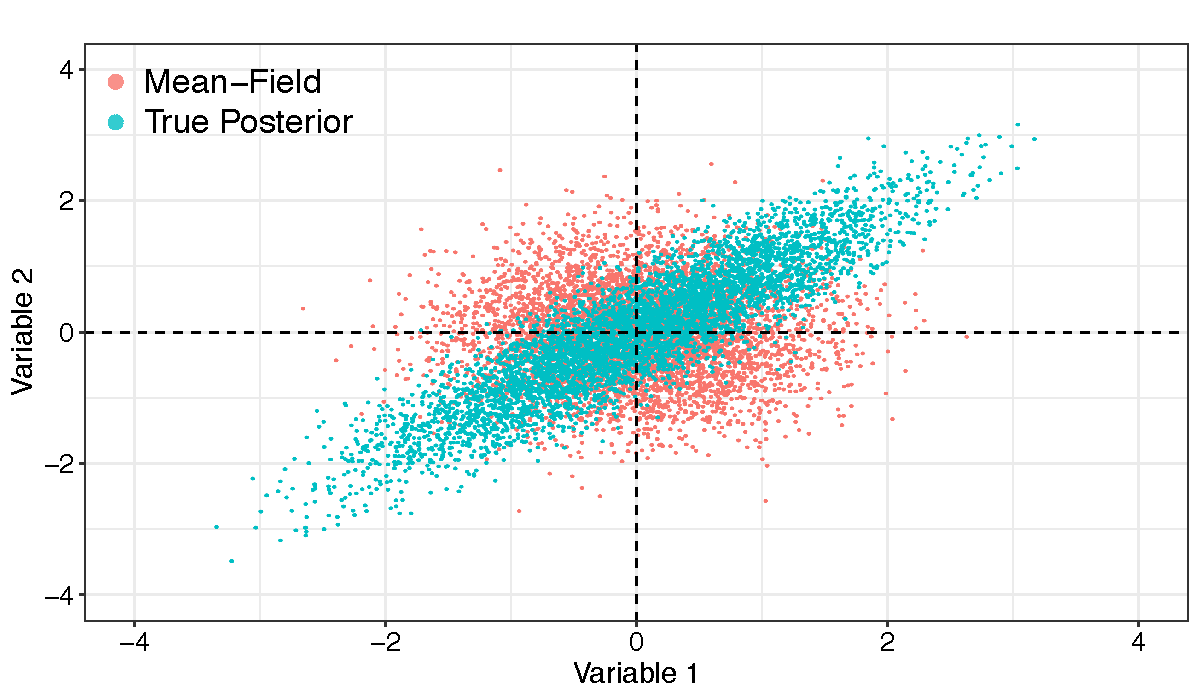
\includegraphics[width=0.7\linewidth]{mean_field}
	\caption{Illustrative example of sampling from a true posterior distribution (blue) versus a fitted mean-field varaitional distribution (red) in a model with two (correlated) unobserved variables. The mean-field approximation wrongly assumes that the unobserved variables are independent.}
	\label{fig:mean_field}
\end{figure}

Using calculus of variations (derivations can be found in \cite{Bishop,Murphy}), it follows that the optimal distribution $q(\bfX)$ that maximises the lower bound $\Lagr(\bfX)$ is
\begin{equation} \label{eq:optimal}
	\log \hat{q}_i(\bfx_i) = \E_{-i} [\log p(\bfY,\bfX)] + \mathrm{const}
\end{equation}
where $\E_{-i}$ denotes an expectation with respect to the $q$ distributions over all variables $\bfx_j$ except for $\bfx_i$.\\
The additive constant is set by normalising the distribution $\hat{q}_i(\bfz_i)$:
\[
	\hat{q}(\bfx_i) = \frac{\exp(\E_{-i}[\log p(\bfY,\bfX)])}{\int \exp(\E_{-i}[\log p(\bfY,\bfX)]) d\bfX}
\]
While the form of $\hat{q}(\bfx_i)$ is not restricted to a specific parametric form, it can be shown that when using conjugate priors, the distributions $\hat{q}_i(\bfx_i)$ have the same functional form as the priors $\hat{p}(\bfx_i)$. 
%An example is shown in Appendix X, but a detailed mathematical treatment with derivations of multiple examples can be found in \cite{Bishop,Murphy,Zhao2009}.


\subsubsection{Fixed-form variational inference}  \label{section:fixed_form}

An alternative and straightforward choice is to directly define a parametric form for the distribution $q(\bfX)$ with some parameters $\bTheta$. Once the choice of $q(\bfX)$ is made, the parameters $\bTheta$ are optimised to minimise $\KL(q(\bfX)||p(\bfX|\bfY))$ (the variational problem):
\begin{align}
	\hat{\bTheta} &= \argmin_{\bTheta} \KL(q(\bfX)||p(\bfX|\bfY)) \\
	&= \E[\log(q(\bfX)) - \log(p(\bfX,\bfY))]
\end{align}
Numerically optimising this function requires the evaluation of expectations with respect to $q(\bfX)$. In closed form, this is only feasable for a limited group of variational distributions. Alternatively, one can attempt Monte Carlo approximations, but in practice this turns to be slow and leads to high-variance estimates \cite{Braun2007,Ranganath2014,Braun2007}.

Typically, one would choose this distribution to factorise over parameters and to be of the same (exponential) family as the prior $p(\bfX)$. In such case there is a closed form coordinate-ascent scheme available, and it turns out that the fixed-form formulation is equivalent to the (non-parametric) mean-field derivation when using conjugate priors.\\
Unfortunately, for generic models with arbitrary families of distributions, no closed-form variational distributions exist \cite{Zhang2017,Blei2016}. 

However, while the parametric assumption certainly limits the flexibility of variational distributions, the advantage of this formulation is that it unveils the possibility to use fast gradient-based methods for the inference procedure \cite{Hoffman2012,Ranganath2014}.

%\paragraph{Black box variational inference}

\subsubsection{Expectation Propagation}  \label{section:expectation_propagation}

Expectation Propagation (EP) is another deterministic strategy with a similar philosophy as the Variational approach. It is also based on minimising the KL divergence between a variational distribution $q(\bfX)$ and the true posterior $p(\bfX|\bfY)$, but while variational inference minimises $KL(p||q)$, EP maximises the reverse KL-divergence $KL(q||p)$.

Interestingly, this simple difference leads to an inference scheme with stringkly different properties. This can be understood by inspecting the differences between the two KL divergence formulas:

Variational inference:
\begin{equation} \label{eq:kl_vb}
	\KL(q(\bfX)||p(\bfX|\bfY)) = - \int_z q(\bfX) \log \frac{p(\bfX|\bfY)}{q(\bfX)}
\end{equation}
Expectation propagation:
\begin{equation} \label{eq:kl_ep}
	\KL(p(\bfX|\bfY)||q(\bfX)) = - \int_z p(\bfX|\bfY) \log \frac{q(\bfX)}{p(\bfX|\bfY)}
\end{equation}
In regions of $\bfX$ where the true posterior density $p(\bfX|\bfY)$ is small, setting a large density for $q(\bfX)$ has a much stronger penalisation in \Cref{eq:kl_ep} than in \Cref{eq:kl_vb}, because of the true posterior density being on the denominator. Hence, EP tends to avoid areas where the density $p(\bfX|\bfY)$ is very low, even if it does not correspond to areas of very high-density in $p(\bfX|\bfY)$. In contrast, in \Cref{eq:kl_vb} there is a strong penalty for having low-density $q(\bfX)$ values.\\
As discussed in \cite{Bishop}, the practical consequences of this duality can be observed when the posterior is multi-modal, as in any sufficiently complex model. In VI, $q(\bfX)$ converges towards areas of high-density in $p(\bfX|\bfY)$, namely local optima. In contrast, EP tends to capture as much non-zero density regions from $p(\bfX|\bfY)$ as possible, thereby averaging across all optima. In the context of doing predictions, the VI solution is much more desirable than the EP solution, as the average of two good parameter values is not necessarily a good parameter itself.\\
A detailed mathematical treatment of EP, including derivations for specific examples, can be found in \cite{Bishop,Murphy,Minka2001}

\begin{figure}[H]
	\centering
	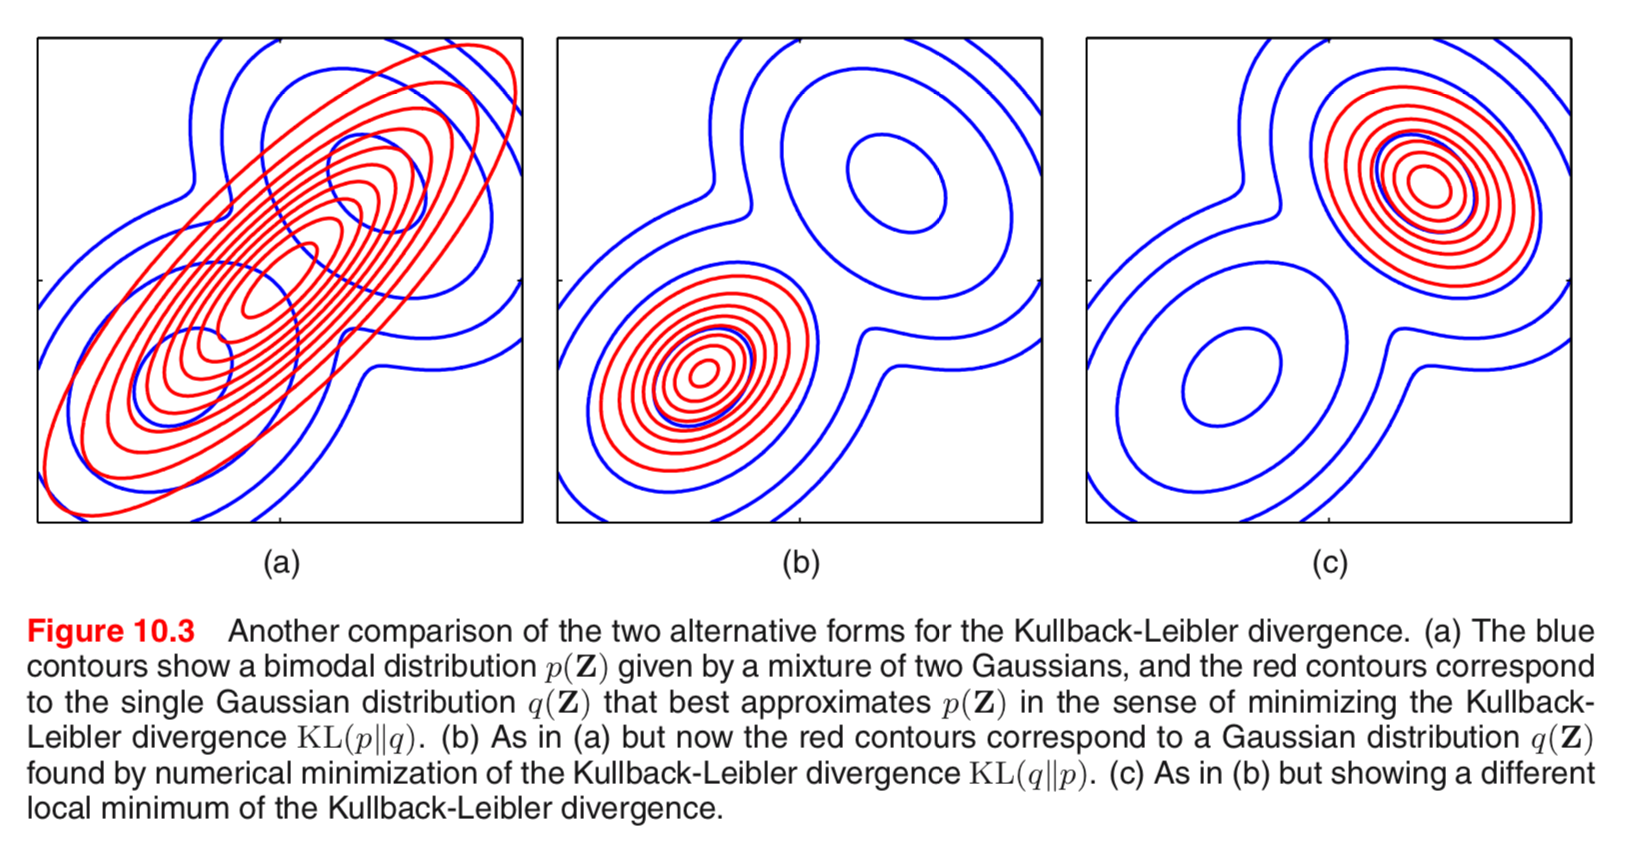
\includegraphics[width=1.0\linewidth]{VB_vs_EP}
	\caption{Illustrative comparison of Variational inference and Expectation Propagation. Shown is the (a) Density and (b) Variance of the true posterior distribution $p(\bfX|\bfY)$ (grey), the variational distribution (orange) and the expectation propagation distribution (green).}
	\label{}
\end{figure}

Following the rationale above, it is easy to predict that variational inference tends to be underestimate the variance of the posterior density. Yet, empirical research have shown that this is acceptable, provided that a good model selection is performed \cite{Blei2006}.


\subsubsection{Conclusions}

In this section we have introduced Bayesian modelling and variational inference methods, which will be used later in this chapter.\\
More generally, variational inference is growing in popularity for the analysis of big data sets and it has been applied to a myriad of different problems, including genome-wide association studies \cite{Carbonetto2012}, population genetics, \cite{Raj2014}, network analysis \cite{Sanguinetti2006} and natural language processing \cite{Blei2003}.

Yet, despite its increasing success, there is significant room for improvement. First and foremost, the theoretical guarantees of variational inference are not as developed as in sampling-based MCMC schemes\cite{Blei2016,Zhang2017,Nakajima2007}. As an example, the mean-field setting makes strong independence assumptions about the parameters.  Although it tends to besurprisingly effective, it is not clear in which applications the dependencies between the parameters are important enough than the mean-field approximation could potentially break.\\
More generally, an open research problem is understanding what are the statistical properties of the variational posterior with respect to the exact posterior \cite{Blei2016,Zhang2017}.

As we shall demonstrate later, alternative strategies have been considered to allow some dependencies between the variables, resulting in \textit{structured} mean-field approximations\cite{Hoffman2014,Titsias2011}. However, they often lead to very complex (if not intractable) inference frameworks. 

Finally, another area of extensive research is how to extend the applicability of VI to non-conjugate models. As discussed in \Cref{section:deterministic_bayesian_inference}, the ELBO of non-conjugate models contains intractable integrals, and setting up an inference scheme requires the use of either stochastic Monte Carlo approximations or deterministic approximations that introduce additional lower bounds \cite{Zhang2017,Seeger2012,Khan2017}. In this thesis we follow this rationale to derive an inference framework for a model with non-gaussian likelihoods.



\subsection{Latent variable models for genomics}

With the exponential growth in the use of high-throughput genomics, biological data sets are increasingly high dimensional, both in terms of samples and features. A key principle of biological data sets is that variation between the features results from differences in underlying, often unobserved, processes. Such processes, whether driven by biological or technical effects, are manifested by coordinated changes in multiple features. This key assumption sets off an entire statistical framework of exploiting the redundancy encoded in the data set to learn the (latent) sources of variation in an unsupervised fashion. This is the aim of dimensionality reduction techniques, or latent variable models \cite{Komili2008, Stegle2012, Leek2007, Pournara2007, Dai2017, Genevieve2018, Meng2016}.


\subsubsection{Mathematical formulation}

Given a dataset $\bfY$ of $N$ samples and $D$ features, latent variable models attempt to exploit the dependencies between the features by reducing the dimensionality of the data to a potentially small set of $K$ latent variables, also called factors. The mapping between the low-dimensional space and the high-dimensional space is performed via a function $f(\bfX|\bTheta)$ that depends on some parameters $\bTheta$.\\
The choice of $f(\bfX|\bTheta)$ is essentially the field of dimensionality reduction. A trade-off exists between complexity and interpretation: while non-linear functions such as deep neural networks provide more explanatory power, this leads to a considerable challenges in interpretation \cite{Zhang2018_NN}. Hence, for most applications where interpretability is essential, $f(\bfX|\bTheta)$ is assumed to be linear:
% \begin{equation} 
% 	y_{nd} = \sum_{k=1}^{K} w_{dk}z_{n,k}
% \end{equation}
\begin{equation} \label{eq:linear_model}
	\mathbf{Y} = \mathbf{Z}\mathbf{W}^{T}
\end{equation}
where $\bfZ \in \R^{N \times K}$ is a matrix that contains the low-dimensional representation for each sample (i.e. the factors). The matrix $\bfW \in \R^{D \times K}$ contains the weights, which provide the linear mapping between the features and the factors.\\
Note that the aim in dimensionality reduction is to exploit the coordinated heterogeneity between features, and hence features are assumed to be centered without loss of generality.

The inference procedure consists in learning the values of all unobserved variables, including factors and weights. As we shall demonstrate, different inference schemes and assumptions on the prior distributions lead to significantly different model outputs \cite{Rattray2009}.


\subsection{Principal Component Analysis} \label{section:pca}

Principal Component Analysis (PCA) is the most popular technique for dimensionality reduction \cite{Hotelling1933,Ringner2008}. Starting from \Cref{eq:linear_model}, two formulations of PCA exist \cite{Bishop2006}. In the maximum variance formulation, the aim is to infer an orthogonal projection of the data onto a low-dimensional space such that variance explained by the projected data is maximised. Formally, 

Formally, the aim in PCA is to infer the matrix $\bfW$ such that the variance of $\bfZ$ (the projected data) is maximised. If we consider a single latent factor, the variance of the projected data is:
\begin{equation*}
	\sigma^2 = \frac{1}{N}\sum_{n=1}^{N} (\bfz_n - \hat{\bfz})^{2} = \frac{1}{N}\sum_{n=1}^{N} (\bfy_n^T \bfw - \hat{\bfy}^T\bfw)^{2}
\end{equation*}

where $\hat{\bfy}$ is a vector with the feature-wise means. If we assumed centered data this simplifies to:
\begin{equation*}
	\sigma^2 = \frac{1}{N}\sum_{n=1}^{N} (\bfy_n^T \bfw)^{2}
\end{equation*}
Some algebra allows us to define this equation in terms of the (centered) data covariance matrix: $\bfS = \frac{1}{N}\sum_{n=1}^{N} \bfy_n\bfy_n^T$:
\begin{align*}
	\sigma^2 &= \frac{1}{N}\sum_{n=1}^{N} (\bfy_n^T \bfw)^T (\bfy_n^T \bfw) \\
	=& (\bfw^T \bfy_n) (\bfy_n^T \bfw) \\
	=& \bfw^T (\bfy_n \bfy_n^T) \bfw \\
	=& \bfw^T \bfS \bfw
\end{align*}

Thus, for a single principal component, the optimisation problem is:
\begin{equation} \label{eq:pca}
	%\argmax_{\|\bfw\|=1} & \sum_{n=1}^{N} (\bfw_1^T \bfy_n)^2 = \\
	\argmax_{\|\bfw\|=1} = \bfw^T \bfS \bfw
\end{equation}

% where $\bfY^T \bfY=\bfS \in \R^{D \times D}$ is the data covariance matrix and $\bfw_1^T$ is the vector of weights. \\
The $k$-th principal component can be found by subtracting from $\bfY$ the reconstructed data by the previous $k-1$ principal components. If we define $\bfz_k=\bfw_k^T \bfY$ to be the $k$-th principal component:
\[
	\hat{\bfY} = \bfY - \sum_{k=1}^{K} (\bfz_k \bfw_k^T)
\]
Re-applying \Cref{eq:pca} defines the new optimisation problem.

In its minimum error formulation, the aim is to find an equivalent projection that minimises the mean squared error between the observations and the data reconstructed using all principal components:
\[
	\argmax_{\|\bfw\|=1} \Vert \bfY - \sum_{k=1}^{K} (\bfz_k \bfw_k^T) \Vert^{2}
\]
where $\Vert \cdot \Vert^{2}$ is the Frobenius norm.

Remarkably, in both cases, solving the optimisation problems via Lagrange multipliers leads to master eigenvalue-eigenvector equation:
\begin{equation}
	\bfS \bfw_k = \lambda_k \bfw_k
\end{equation}
where the weight vectors $\bfw_k$ can be calculated as the eigenvectors of the covariance matrix $\bfS$ \cite{Bishop2006}.

Interestingly, the reason why the maximum variance solution and the minimum reconstruction error solution are the same can be understood by applying Pythagoras theorem to the right triangle defined by the projection of a sample $\bfy_{n}$ to a weight vector $\bfw$ (\Cref{fig:pca2}).
Assuming again centered data, the variance of $\bfy_{n}$ is $\|\bfy_{n}\| = \bfy_{n}^T \bfy_{n}$. This variance decomposes as the sum of the variance in the latent space $\|\bfz_{n}\| = \bfz_{n}^T \bfz_{n}$ and the residual variance after reconstruction $\|\bfy_{n} - \bfz_{n} \bfw^T \|$:

\begin{figure}[H]
	\centering
	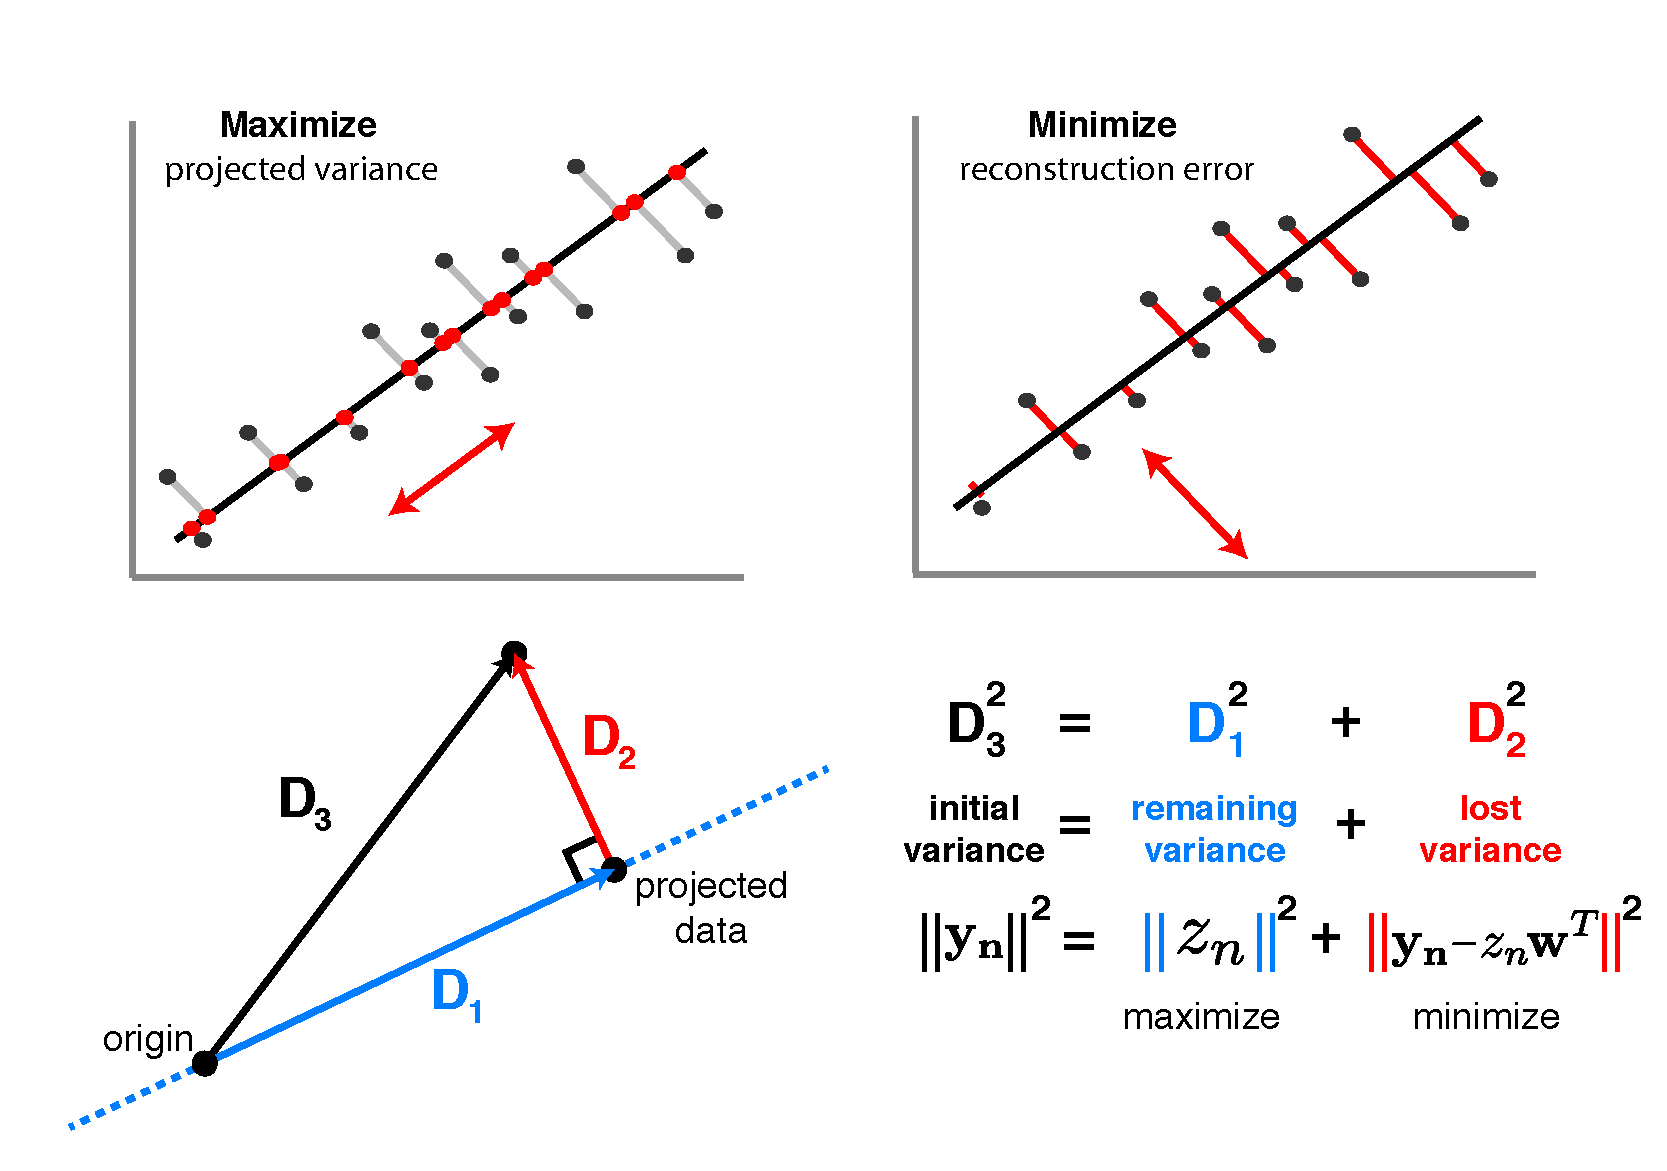
\includegraphics[width=0.8\linewidth]{pca2}
	\caption[Maximizing the variance in the principal component space is equivalent to minimizing the data reconstruction error]{In the maximum variance formulation the aim is to maximise the variance of the projected data (blue line), whereas in the minimum error formulation the aim is to minimise the residual variance (red line). Given a fixed total variance (black line), both strategies are equivalent}
	\label{fig:pca2}
\end{figure}

The main strength of PCA relies on its simplicity and closed form solution. Additionally, the linear mapping has the advantage of yielding interpretable feature weights, so that inspection of $\bfw_k$ reveals which features are jointly affected by the $k$-th principal component.\\
However, PCA suffers from serious drawbacks when applying it to real data sets \cite{Li2017b}. First, biological measurements are inherently noisy, and there is no explicit account of noise in PCA. In practice, high variance components are often asociated with signal whereas low-variance components are assumed to be noise, but an ideal model should explicitly disentangle the uncoordinated variability that is attributed to noise from the coordinated variability that is characterised as signal. Second, in its original formulation, no missing data is allowed \cite{Ilin2010}. Third, it does not offer a principled way of modelling prior information about the data.

\subsection{Probabilistic Principal Component Analysis and Factor Analysis} \label{section:probabilistic_pca}
A probabilistic version of PCA was initially proposed in \cite{Tipping1999}. It can be formulated by converting some (or all) fixed parameters into random variables and adding an explicit noise term to \Cref{eq:linear_model}:
\begin{equation}
	\bfY = \bfW \bfZ + \bepsilon
\end{equation}
where the weights $\bfW$ are assumed to be non-probabilistic parameters, but the noise $\bepsilon$ and the latent variables $\bfZ$ (the principal components) are assumed to follow an isotropic normal distribution:
\begin{align*}
	p(\bfZ) &= \prod_{n=1}^{N} \prod_{k=1}^{K} \Ndist{z_{nk}}{0,1} \\
	p(\epsilon) &= \Ndist {\epsilon}{0,\sigma^2}
\end{align*}
%The alternative strategy of treating $\bfZ$ as random variables and $\bfW$ as parameters has also been explored \cite{Lawrence2005}.\\

All together, this leads to a normally-distributed likelihood:
\begin{equation} \label{eq:ppca_lik}
	% p(\bfY|\bfW,\bfZ,\sigma) = \Ndist{\bfY}{\bfW \bfZ,\sigma^2 \I}
	p(\bfY|\bfW,\bfZ,\sigma) = \prod_{n=1}^{N} \prod_{d=1}^{D} \Ndist{y_{n,d}}{\bfw_{,:k}^T \bfz_{n,:},\sigma^2 \I}
\end{equation}

The corresponding graphical model is:

\begin{figure}[H]
	\centering
	% \input{graphical_models/colours}

\begin{tikzpicture}

% Define nodes
\node[obs]   (Y) {$y_{n,d}$};
\node[latent, xshift=-1.5cm, above=of Y, yshift=-0.4cm] (Z) {$z_{n,k}$};
\node[latent, double, double distance=1pt, above=of Y, yshift=0.6cm] (W) {$w_{d,k}$};
\node[latent, double, double distance=1pt, xshift=1.5cm] (Tau) {$\tau$};

% Connect the nodes
\edge {Z,W, Tau} {Y};

% Plates
\plate[] {plateK} {(Z)(W)} {$K$};
\plate[] {plateN} {(Y)(Z)(plateK.south east)(plateK.south west)} {$N$};
\plate[] {plateD} {(Y)(W)(plateK.north east)(plateN.south east)} {$D$};

\end{tikzpicture}
	\caption{Graphical model for probabilistic PCA. The latent variables are modelled as random variables, whereas the weights and the noise are modelled as deterministic parameters.}
	\label{fig:pPCA}
\end{figure}

Importantly, the choice of the distribution for $\epsilon$ implies that the noise of each feature is independent but restricted to have the same variance $\sigma^2$. In practice this is a limiting assumption, as different features are expected to show different degrees of noise, albeit this constraint can be relaxed and forms the basis of Factor Analysis \cite{Rubin1982,Bishop2006}.

The inference procedures involves learning the parameters $\bfW$, and $\sigma^2$ and a posterior probability distribution for $\bfZ$. As the model depends on latent variables, inference can be performed using the iterative Expectation-Maximisation (EM) algorithm \cite{Rubin1982,Bishop2006}. In the expectation step, the posterior distribution for $\bfZ$ is computed in closed form (due to conjugacy between the likelihood and the prior), given current estimates for the parameters $\bfW$, and $\sigma^2$. In the maximisation step, the parameters are calculated by maximising the expectation of the joint log likelihood under the posterior distribution of $\bfZ$ found in the E step \cite{Tipping1999}.\\
Interestingly, the EM solution of probabilistic PCA lies in the same subspace as the traditional PCA solution \cite{Tipping1999}, but the use of a probabilistic framework brings several benefits. First, model selection can be performed by comparing likelihoods across different settings of parameters. Second, missing data can naturally be accounted for by ignoring the missing observations from the likelihood. Finally, the probabilistic formulation sets the core framework for a Bayesian treatment of PCA, enabling a broad range of principled extensions tailored different types of data sets.


\subsection{Bayesian Principal Component Analysis and Bayesian Factor Analysis} \label{section:bayesian_pca}

The full Bayesian treatment of PCA requires the specification of prior probability distributions for all unobserved variables:
\begin{align*}
	p(\bfZ) &= \prod_{n=1}^{N} \prod_{k=1}^{K} \Ndist{z_{nk}}{0,1} \\
	p(\bfW) &= \prod_{d=1}^{D} \prod_{k=1}^{K} \Ndist{w_{dk}}{0,1} \\
	p(\epsilon) &= \Ndist {\epsilon}{0,\tau^{-1}} \\
	p(\tau) &= \Gdist{\tau}{a_0,b_0}
\end{align*}
where $\tau$ is the precision (inverse of the variance) of the noise term. A generalisation to Bayesian Factor Analysis follows by allowing a separate noise term per feature:
\begin{align*}
	p(\bepsilon) &= \prod_{d=1}^{D} \Ndist {\epsilon_d}{0,\tau_d^{-1}} \\
	p(\btau) &= \prod_{d=1}^{D} \Gdist{\tau_d}{a_0,b_0}
\end{align*}
where $a_0$ and $b_0$ are fixed hyperparameters. As in \Cref{eq:ppca_lik}, this results in a Normal likelihood:
\[
	p(\bfY|\bfW,\bfZ,\btau) = \prod_{n=1}^{N} \prod_{d=1}^{D} \Ndist{y_{nd}}{\bfw_{d}^T \bfz_{n},\tau_d}
\]

The corresponding graphical model is:

\begin{figure}[H] 
	\centering
	\begin{tikzpicture}

% Define nodes
\node[obs]   (Y) {$y_{n,d}$};
\node[latent, above=of Y, xshift=-1.5cm] (Z) {$z_{n,k}$};
\node[latent, above=of Y, xshift=1.5cm] (W) {$w_{d,k}$};
\node[latent, xshift=1.5cm] (Tau) {$\tau_{d}$};

% Connect the nodes
\edge {Z,W, Tau} {Y};

% Plates
\plate[] {plateK} {(Z)(W)} {$K$};
\plate[] {plateN} {(Y)(Z)(plateK.north west)} {$N$};
\plate[] {plateD} {(Y)(W)(Tau)(plateK.south east) (plateN.south east) (plateN.north east)} {$D$};

\end{tikzpicture}
	\caption{Graphical model for Bayesian Factor Analysis. All unobserved variables are modelled as random variables.}
	\label{fig:bayesianFA}
\end{figure}


\subsection{Hierarchical priors}  \label{section:hierarchical_priors}

A key advantage of the full Bayesian treatment is that it explicitly captures uncertainity on the estimation of all unobserved variables, as opposed to the probabilistic PCA model \cite{Bishop1999a,Bishop1999b}. Yet, more importantly, the use of (hierarchical) prior distributions allow different modelling assumptions to be encoded, providing a flexible and principled approach to extend PCA to a myriad of modelling scenarios, including multi-view generalisations \cite{Klami2008,Virtanen2012,Klami2015,Bunte2016,Khan2014,Zhao2016}.

\subsubsection{Automatic relevance determination} \label{section:ard}


As an example, a major challenge in PCA is how to determine the dimensionality of the latent space (i.e. the number of principal components). As we will show, the use of hierarchical prior distributions allows the model to introduce sparsity assumptions on the weights in such a way that the model automatically learns the number of factors.\\
In the context of Factor Analysis, one the first sparsity priors to be proposed was the Automatic Relevance determination (ARD) prior \cite{Neal1995,Mackay1996,Bishop1999a,Bishop1999b}. 
\begin{equation*} \label{eq:ard}
	p(\bfW|\balpha) = \prod_{k=1}^{K} \Ndist{\bfw_{:,k}}{0,\frac{1}{\alpha_{k}}\I_{D}} \\
	\qquad\qquad
	p(\balpha) = \prod_{k=1}^{K} \Gdist{\alpha_k}{a_0^\alpha, b_0^\alpha}
\end{equation*}
The aim of this prior is two-fold. First, the zero-mean normal distribution specifies that, \textit{a priori}, no information is available and all features are \textit{inactive}. When exposed to some data, the posterior distribution for $\bfW$ will be estimated by weighting the contribution from the likelihood, potentially allowing features to escape from the zero-centered prior (\Cref{fig:ard}).\\
Second, performing inference on the variable $\balpha = \{ \alpha_1, \cdots, \alpha_k \}$ enables the model to discard inactive factors. To understand this, let us assume that only $K=5$ true factors exist, but the model is initialised with $K=20$ factors. In such case, inactive factors can be prunned out by driving the corresponding $\alpha_k$ to infinity. In turn, this causes the posterior $p(\bfw_{:,k}|\bfY)$ to be sharply peaked at zero, resulting in the inactivation of all its weights. %\Cref{fig:hinton}.

\begin{figure}[H] \begin{center}
	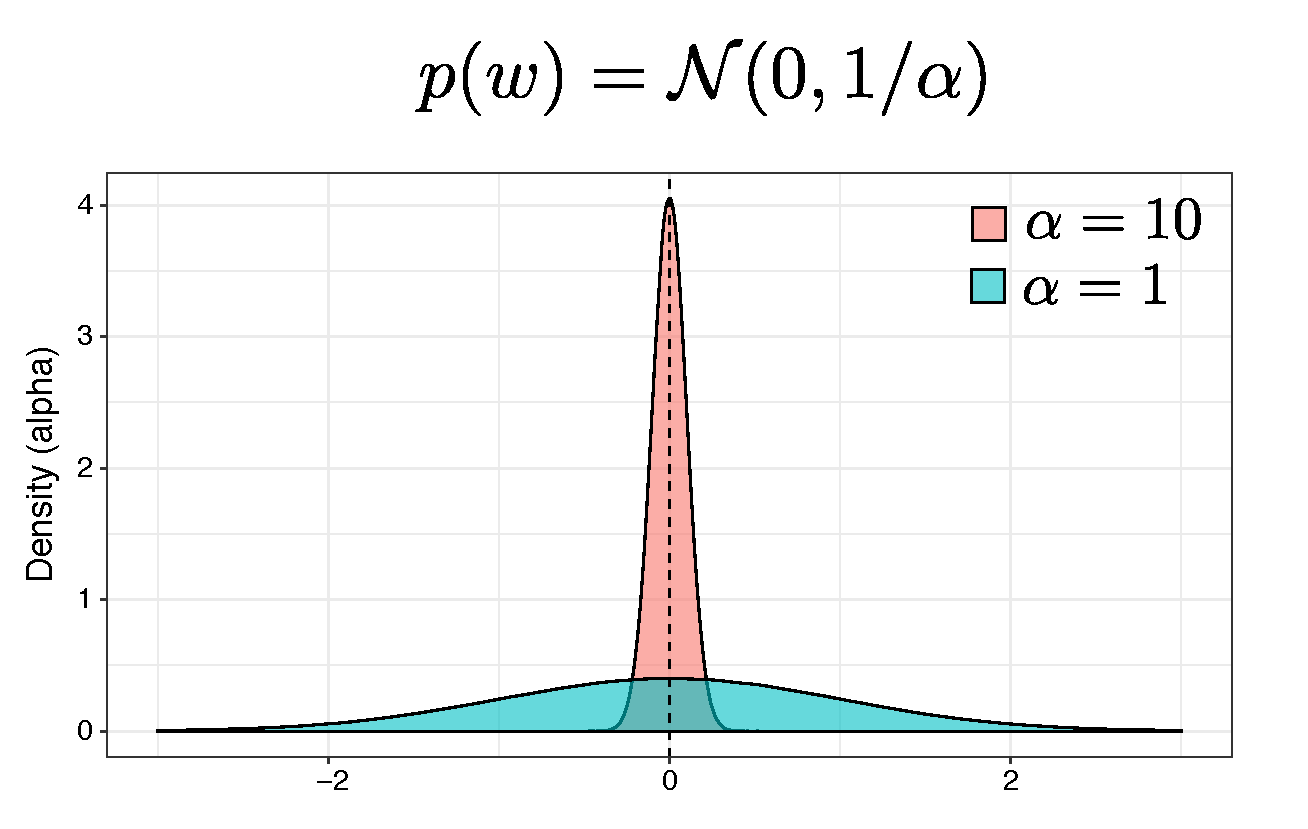
\includegraphics[width=0.7\textwidth]{Chapter2/Figs/ard}
	\caption{Visualisation of the sparsity-inducing Automatic Relevance Determination prior}
	\label{fig:ard}
\end{center} \end{figure}

% \begin{figure}[H] \begin{center}
% 	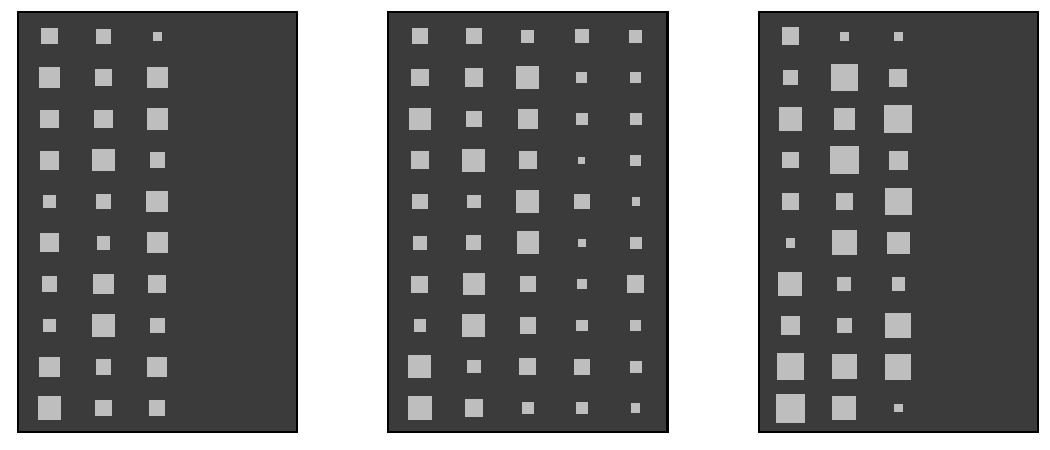
\includegraphics[width=0.8\textwidth]{Chapter2/Figs/hinton}
%             \caption[Hinton plot of the weight matrix for a Bayesian Factor Analysis model with an ARD prior]{Hinton plots display the values of the weight matrix, similar to a heatmap, where bigger squares depict larger weights. Shown are the Hinton plots for (a) the true weights, (b) the infered weights by a Factor Analysis model with no ARD prior (middle), and (c) the infered weights by a Factor Analysis model with ARD prior per factor. This figure was generated using simulated data with $N=100$ samples, $D=10$ features and $K=3$ factors.}
% 	\label{fig:hinton}
% \end{center} \end{figure}

\subsubsection{Spike-and-slab prior} \label{section_spikeslab}

Sparse extensions of the Bayesian factor analysis model have been proposed as a regularisation mechanism but also to model inherent assumptions regarding the sparse nature of biological data \cite{Stegle2012,Gao2013}.\\
The variability observed in biological data is driven both by technical factors and biological factors. Technical factors (i.e. batch effects) tend to be relatively strong and alter the expression of a large proportion of genes, whereas the biological factors are potentially weak effects driven by changes in small gene regulatory networks \cite{Gao2013}. Hence, a practical factor analysis model should be able to learn factors with different degrees of sparsity.\\
The ARD prior proposed in \Cref{eq:ard} allows entire factors to be dropped out from the model, but it provides a weak degree of regularisation when it comes to inactivating individual weights within the active factors.

A sparse generalisation of the Factor Analysis model proposed above can be achieved by combining the ARD prior with a spike-and-slab prior \cite{Mitchell1988,Titsias2011}:
\begin{align}
	p(w_{d,k} \mid \alpha_k,\theta_k) &= (1-\theta_k) \mathds{1}_0(w_{d,k}) + \theta_k \Ndist{w_{d,k}}{0, \alpha_k^{-1}} \\
	p(\theta_k) &= \Bdist{\theta_k}{a_0^\theta,b_0^\theta} \\
	p(\alpha_k) &= \Gdist{\alpha_k}{a_0^\alpha, b_0^\alpha}
\end{align}

The corresponding graphical model is:

\begin{figure}[H] \begin{center}
	\begin{tikzpicture}

% Define nodes
\node[obs]   (Y) {$y_{n,d}$};
\node[latent, above=of Y, xshift=-1.5cm] (Z) {$z_{n,k}$};
\node[latent, above=of W, xshift=-0.75cm] (Theta) {$\theta_{k}$};
\node[latent, above=of W, xshift=0.75cm] (Alpha) {$\alpha_{k}$};
\node[latent, above=of Y, xshift=1.5cm] (W) {$w_{d,k}$};
\node[latent, xshift=1.5cm] (Tau) {$\tau_{d}$};

% Connect the nodes
\edge {Theta, Alpha} {W};
\edge {Z, W, Tau} {Y};

% Plates
\plate[] {plateK} {(Z)(W)(Theta)(Alpha)} {$K$};
% \plate[] {plateN} {(Y)(Z)(plateK.north west)} {$N$};
\plate[] {plateN} {(Y)(Z)} {$N$};
\plate[] {plateD} {(Y)(W)(Tau)(plateK.south east) (plateN.south east) (plateN.north east)} {$D$};

\end{tikzpicture}
	\label{fig:bayesianFA}
	\caption{Graphical model for Bayesian sparse Factor Analysis. A double sparsity-inducing prior is used on the weights: an ARD prior to prune inactive factors and a spike-and-slab prior to inactive individual features within the active factors.}
\end{center} \end{figure}

The spike-and-slab prior is effectively a mixture model where features are sampled from a zero-inflated Gaussian distribution, where $\theta_k \in (0,1)$ dictates the level of sparsity per factor (i.e. how many active features). A value of $\theta_k$ close to $0$ implies that most of the weights of factor $k$ are shrunk to $0$ (i.e. a sparse factor), whereas a value of $\theta_k$ close to $1$ implies that most of the weights are non-zero (i.e. dense factors). By learning $\theta_k$ from the data, the model naturally accounts for combinations of sparse and dense factors.


% \subsubsection{Inference}
% In a fully Bayesian setting, the inference procedure corresponds to learning the posterior distributions for each unobserved variable. However, applying Bayes rule yields an analytically intractable solution, and approximate methods are required. This is discussed in Chapter X.



\subsection{Multi-view factor analysis models}

Probabilistic PCA and Factor Analysis perform dimensionality reduction from a single input matrix. In some occasions data is collected from multiple data sources that exibit heterogeneous statistical properties, resulting in a structured data set where features are naturally partitioned into views \cite{Xu2013,Li2016,Zeng2018}. A clear biological example is multi-omics data, where, for the same set of samples, multiple molecular layers are profiled. Each of the data modalities can be analysed separately using conventional (single-view) methods, but in the ideal strategy a single model should be used to leverage information across all molecular layers using a flexible and principled approach. This is referred to as the multi-view learning problem \cite{Xu2013,Li2016}.\\
A tempting approach to circumvent the multi-view learning problem is to simply concatenate all data sets before applying conventional (single-view) latent variable models \cite{Ritchie2015}. However, this is prone to fail for several reasons. First, heterogeneous data modalities cannot always be modelled using the same likelihood function. For example, continuous measurements are often modelled using a normal distribution, but binary and count-based traits are not appropriately modelled by this distribution \cite{Pilling2018}. Second, even if all views are modelled with the same likelihood, differences in the scale and the magnitude of the variance can lead to some views being overrepresented in the latent space. Finally, in a multi-view data set we expect multiple sources of variation, some driven by a single view, whereas others could capture shared variability across multiple views. In other words, from a structured input space, one can also expect a structured latent representation. Not taking this behaviour into account can lead to challenges in the interpretability of the latent space.

A comprehensive review of multi-view machine learning methods can be found in \cite{Xu2013} and a more genomics-oriented perspective in \cite{Ritchie2015}. For the purpose of this thesis, I will describe only the use of latent variable models for multi-view data integration.

\subsection{Canonical Correlation Analysis} \label{cca}

Canonical Correlation Analysis (CCA) is a simple extension of PCA to find linear components that capture correlations between two datasets \cite{Hotteling1936,Hardle2007}.\\
Given two data matrices $\bfY_1 \in \R^{N \times D_1}$ and $\bfY_2 \in \R^{N \times D_2}$ CCA finds a set of linear combinations $\bfU \in \R^{D_1 \times K}$ and $\bfV \in \R^{D_2 \times K}$ with maximal cross-correlation.
For the first pair of canonical variables, the optimisation problem is:
\[
	(\hat{\bfu_1}, \hat{\bfv_1}) = \argmax_{\bfu_1,\bfv_1} corr(\bfu_{1}^T \bfY_1, \bfv_{1}^T \bfY_2)
\]
As in conventional PCA, the linear components are constraint to be orthogonal. Hence, the first pair of canonical variables $\bfu_1$ and $\bfv_1$ contain the linear combination of variables that have maximal correlation. Subsequently, the second pair of canonical variables $\bfu_2$ and $\bfv_2$ is found from the residuals of the first canonical variables.

Given the similarity with PCA, both methods share statistical properties, including the linear mapping between the low-dimensional space and the high-dimensional space, and the closed-form solution using singular value decomposition \cite{Hotteling1936,Hardle2007}.\\
Because of its simplicity and efficient computation, CCA has widespread use as a dimensionality reduction technique \cite{Hardle2007}. Yet, as expected, CCA suffers from the same pitfalls as PCA: difficulties in selecting the number of components, lack of sparsity in the solutions and absence of probabilistic formulation. In addition, CCA have been shown to overfit for datasets where $D>>N$ \cite{McCabe2018,Guo2016}. Hence, probabilistic versions with sparsity assumptions that reduce overfitting and improve interpretability followed.


\subsubsection{Probabilistic Canonical Correlation Analysis} \label{section_probabilisticCCA}

Following the derivation of probabilistic PCA \cite{Tipping1999}, a similar effort enabled a probabilistic formulation of CCA as a generative model \cite{Bach2005}.\\
In this model, the two matrix of observations $\bfY^{1}$ and $\bfY^{2}$ are decomposed in terms of two weight matrices $\bfW^{1}$ and $\bfW^{2}$ but a joint latent matrix $\bfZ$:
\begin{align*}
	\bfY^{1} &= \bfW^{1} \bfZ + \epsilon^{1} \\
	\bfY^{2} &= \bfW^{2} \bfZ + \epsilon^{2}
\end{align*}
With the following prior probability distributions:
\begin{align*}
	p(z_{nk}) &= \Ndist{z_{nk}}{0,1} \\
	p(\epsilon^{1}) &= \Ndist {\epsilon^{1}}{\tau_{1}^{-1}} \\
	p(\epsilon^{2}) &= \Ndist {\epsilon^{2}}{\tau_{2}^{-1}}
\end{align*}
As in \cite{Tipping1999}, the weights and the variance of the noise are assumed to be non-probabilistic parameters, whereas the factors are probabilistic unobserved variables. This yields the following likelihood functions:
\begin{align} \label{eq:probabilistic_cca_likelihood}
	p(\bfY^{1}|\bfW^{1},\bfZ,\tau_{1}) &= \prod_{n=1}^{N} \prod_{d=1}^{D_1} \Ndist{y^{1}_{n,d}}{(\bfw_{:,k}^{1})^T \bfz_{n},\tau_{1}^{-1}} \\
	p(\bfY^{2}|\bfW^{2},\bfZ,\tau_{2}) &= \prod_{n=1}^{N} \prod_{d=1}^{D_2} \Ndist{y^{2}_{n,d}}{(\bfw_{:,k}^{2})^T \bfz_{n},\tau_{2}^{-1}} \nonumber
\end{align}

The corresponding graphical model is:
\begin{figure}[H] \begin{center}
	\begin{tikzpicture}

% Define nodes
\node[obs, xshift=-1.5cm] (Y1) {$y^{1}_{n,d}$};
\node[obs, xshift=+1.5cm] (Y2) {$y^{2}_{n,d}$};

\node[latent, below=of Y1, yshift=+0.5cm, xshift=+1.5cm] (Z) {$z_{n,k}$};

\node[latent, double, double distance=1pt, below=of Y1, xshift=-1cm, yshift=-1cm] (W1) {$w^{1}_{d,k}$};
\node[latent, double, double distance=1pt, below=of Y2, xshift=+1cm, yshift=-1cm] (W2) {$w^{2}_{d,k}$};

\node[latent, double, double distance=1pt, left=of Y1, yshift=-0.5cm] (Tau1) {$\tau^{1}$};
\node[latent, double, double distance=1pt, right=of Y2, yshift=-0.5cm] (Tau2) {$\tau^{2}$};

% Connect the nodes
\edge {Z} {Y1};
\edge {Z} {Y2};
\edge {W1} {Y1};
\edge {W2} {Y2};
\edge {Tau1} {Y1};
\edge {Tau2} {Y2};
% \edge {Z,W, Tau} {Y};

% Plates
\plate[] {plateK} {(Z)(W1)(W2)} {$K$};
% \plate[] {plateN} {(Y1)(Y2)(Z)(plateD1.north)} {$N$};
% \plate[] {plateD1} {(Y1)(W1)(plateK.south)(plateN.north)} {$D_1$};
% \plate[] {plateD2} {(Y2)(W2)(plateK.south)(plateN.north)} {$D_2$};
\plate[] {plateN} {(Y1)(Y2)(Z)} {$N$};
\plate[] {plateD1} {(Y1)(W1)(Tau1)} {$D_1$};
\plate[] {plateD2} {(Y2)(W2)(Tau2)} {$D_2$};

\end{tikzpicture}



	\label{fig:graphical_CCA}
	\caption{Graphical model for probabilistic Canonical Correlation Analysis}
\end{center} \end{figure}

Notice that the observations for both data sets are generated from the same set of latent variables $\bfZ$. This ensures that the model is focused on capturing the variation associated with cross-correlated groups of features.

Analogously to probabilistic PCA, the expected value of the posterior distribution $p(\bfZ|\bfY^{1},\bfY^{2})$ span the same subspace as standard CCA \cite{Bach2005}. Nonetheless, one of the many advantage of a probabilistic formulation is that it enables a broad range of principled extensions into larger graphical models.


\subsubsection{Bayesian Canonical Correlation Analysis} \label{section:bayesian_cca}

A fully Bayesian treatment of CCA followed based on exactly the same principle presented in \Cref{section:bayesian_pca} by introducing prior distributions to all unobserved variables \cite{Wang2007,Klami2013}:
\begin{align*} 
	p(\bfZ) &= \prod_{n=1}^{N} \prod_{k=1}^{K} \Ndist{z_{nk}}{0,1} \\
	p(\epsilon^{1}) &= \Ndist {\epsilon^{1}}{\sigma_{1}^{2}} \\
	p(\epsilon^{2}) &= \Ndist {\epsilon^{2}}{\sigma_{2}^{2}} \\
	p(\bfW^1|\balpha) &= \prod_{k=1}^{K} \Ndist{\bfw^{1}_{:,k}}{0,\frac{1}{\alpha_{k}}\I_{D_1}} \\
	p(\bfW^2|\balpha) &= \prod_{k=1}^{K} \Ndist{\bfw^{2}_{:,k}}{0,\frac{1}{\alpha_{k}}\I_{D_2}} \\
	p(\balpha) &= \prod_{k=1}^{K} \Gdist{\alpha_k}{a_0^\alpha, b_0^\alpha}
\end{align*}
Resulting in the same likelihood model as in \Cref{eq:probabilistic_cca_likelihood}. Yet, notice that an ARD is introduced per factor, allowing an automatic inference of the dimensionality in the latent subspace.
Also, there is some flexibility in the definition of noise. Whereas an independent noise term can be defined per view, one can also model correlated noise by introducing a multivariate Gaussian distribution with full-rank covariance \cite{Wang2007,Klami2013}.

The corresponding graphical model is:
\begin{figure}[H] \begin{center}
	\begin{tikzpicture}

% Define nodes
\node[obs, xshift=-1.5cm] (Y1) {$y^{1}_{n,d}$};
\node[obs, xshift=+1.5cm] (Y2) {$y^{2}_{n,d}$};

\node[latent, below=of Y1, yshift=+0.5cm, xshift=+1.5cm] (Z) {$z_{n,k}$};

\node[latent, below=of Y1, xshift=-1cm, yshift=-1cm] (W1) {$w^{1}_{d,k}$};
\node[latent, below=of Y2, xshift=+1cm, yshift=-1cm] (W2) {$w^{2}_{d,k}$};

\node[latent, left=of Y1, yshift=-0.5cm] (Tau1) {$\tau^{1}$};
\node[latent, right=of Y2, yshift=-0.5cm] (Tau2) {$\tau^{2}$};

% Connect the nodes
\edge {Z} {Y1};
\edge {Z} {Y2};
\edge {W1} {Y1};
\edge {W2} {Y2};
\edge {Tau1} {Y1};
\edge {Tau2} {Y2};
% \edge {Z,W, Tau} {Y};

% Plates
\plate[] {plateK} {(Z)(W1)(W2)} {$K$};
% \plate[] {plateN} {(Y1)(Y2)(Z)(plateD1.north)} {$N$};
% \plate[] {plateD1} {(Y1)(W1)(plateK.south)(plateN.north)} {$D_1$};
% \plate[] {plateD2} {(Y2)(W2)(plateK.south)(plateN.north)} {$D_2$};
\plate[] {plateN} {(Y1)(Y2)(Z)} {$N$};
\plate[] {plateD1} {(Y1)(W1)(Tau1)} {$D_1$};
\plate[] {plateD2} {(Y2)(W2)(Tau2)} {$D_2$};

\end{tikzpicture}
	\label{fig:graphical_bayesianCCA}
	\caption{Graphical model for Bayesian Canonical Correlation Analysis}
\end{center} \end{figure}

As expected, the sparsity priors yield a more sparse solution than traditional CCA, which is more appropriate for biological data analysis. However, this solution is still limited to $M=2$ views, which leads us to the next model extension.

% (\Cref{fig:hinton_cca}):
% \begin{figure}[H]
% 	\centering
% 	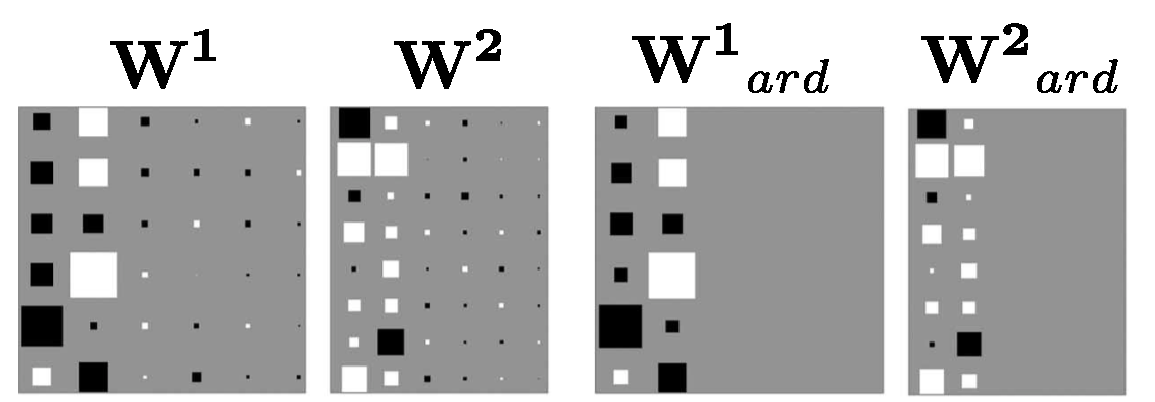
\includegraphics[width=0.85\linewidth]{hinton_cca}
% 	\caption{Comparison of the Hinton's diagram of $\bfW^{1}$ and $\bfW^{2}$ for the maximum likelihood CCA model (two left plots) and the variational Bayes CCA model (two right plots). Reprinted from \cite{Wang2007} with modifications.}
% 	\label{fig:hinton_cca}
% \end{figure}


\subsection{Group Factor Analysis} \label{section:gfa}

Group Factor Analysis (GFA) is the natural generalisation of Bayesian Canonical Correlation Analysis to an arbitrary number of views.
The original idea was originally presented in \cite{Virtanen2012} and a series of generalisations followed, tailored with specific assumptions for different applications \cite{Klami2015,Leppaaho2017,Bunte2016,Khan2014,Zhao2016,Remes2015}. In this section we will outline the core principle of GFA.

Given a data set of $M$ views $\bfY_1, \cdots, \bfY_M$, the task of GFA is to find $K$ factors that capture the variability \textit{within} as well as the variability \textit{between} views. In other words, we want to capture factors that not only explain variance that is shared across all views but we also want to capture factors that explain variance within a single view or between different subsets of views.\\
The starting point is to generalise the Bayesian CCA model (\Cref{section:bayesian_cca}) to $M$ views:
\begin{align*}
	\bfY^{1} &= \bfW^{2} \bfZ + \epsilon^{1} \\
	\bfY^{2} &= \bfW^{2} \bfZ + \epsilon^{2} \\
	& \cdots \\
	\bfY^{M} &= \bfW^{M} \bfZ + \epsilon^{M}
\end{align*}
Notice that there is a common factor space for all views, but there is a view-specific weight matrix. The key to disentangle the activity of each factor in each view lies on the sparsity structure imposed in the weights. Intuitively, if a factor $k$ is not driving any variation in a specific view $m$ we want all the individual weights to be pushed to zero. As shown before, this behaviour can be achieved using Automatic Relevance Determination (ARD) priors. However, if we were to use the same approach as in Bayesian CCA, where the ARD prior for factor $k$ is shared across all views, then factors would be restricted to have the same activity across all views.\\
In GFA this is generalised as follows:
\begin{align}
	p(\bfW) &= \prod_{m=1}^{M} \prod_{k=1}^{K} \Ndist{\bfw_{:,k}^m}{0,\frac{1}{\alpha_k^m}} \\
	p(\balpha) &= \prod_{m=1}^{M} \prod_{k=1}^{K} \Gdist{\alpha_k^m}{a_0^\alpha, b_0^\alpha}
\end{align}
This is effectively setting an ARD prior per factor $k$ and view $m$. The matrix $\balpha \in \R^{M \times K}$ defines four types of factors: (1) Inactive factors that do not explain variance in any view, which corresponds to all values $\balpha_k$ being large. (2) Fully shared factors that explain variance across all views, which corresponds to all values $\balpha_k$ being small. (3) Unique factors that explain variance in a single view, which corresponds to all values $\balpha_k$ being large, except for one entry. (4) Partially shared factors that explain variance in a subsets views, which corresponds to a mixture of small and large values for $\balpha_k$.\\

The corresponding graphical model is:

\begin{figure}[H] \begin{center}
	% \begin{tikzpicture}

% % Define nodes
% \node[obs, xshift=-1.5cm] (Y1) {$y^{m}_{n,d}$};

% \node[latent, below=of Y1, yshift=+0.5cm, xshift=+1.5cm] (Z) {$z_{n,k}$};

% \node[latent, double, double distance=1pt, below=of Y1, xshift=-1cm, yshift=-1cm] (W1) {$w^{1}_{d,k}$};
% \node[latent, double, double distance=1pt, below=of Y2, xshift=+1cm, yshift=-1cm] (W2) {$w^{2}_{d,k}$};

% \node[latent, double, double distance=1pt, left=of Y1, yshift=-0.5cm] (Tau1) {$\tau^{1}$};
% \node[latent, double, double distance=1pt, right=of Y2, yshift=-0.5cm] (Tau2) {$\tau^{2}$};

% % Connect the nodes
% \edge {Z} {Y1};
% \edge {Z} {Y2};
% \edge {W1} {Y1};
% \edge {W2} {Y2};
% \edge {Tau1} {Y1};
% \edge {Tau2} {Y2};
% % \edge {Z,W, Tau} {Y};

% % Plates
% \plate[] {plateK} {(Z)(W1)(W2)} {$K$};
% % \plate[] {plateN} {(Y1)(Y2)(Z)(plateD1.north)} {$N$};
% % \plate[] {plateD1} {(Y1)(W1)(plateK.south)(plateN.north)} {$D_1$};
% % \plate[] {plateD2} {(Y2)(W2)(plateK.south)(plateN.north)} {$D_2$};
% \plate[] {plateN} {(Y1)(Y2)(Z)} {$N$};
% \plate[] {plateD1} {(Y1)(W1)(Tau1)} {$D_1$};
% \plate[] {plateD2} {(Y2)(W2)(Tau2)} {$D_2$};

% \end{tikzpicture}



\begin{tikzpicture}
  % Define nodes:
  % matrix factorisation level
  \node[obs]   (Y) {$y_{n,d}^m$};
  \node[latent, above=of Y, xshift=-1.5cm] (Z) {$z_{n,k}$};
  \node[latent, above=of Y, xshift=1.5cm] (W) {$w^m_{k,d}$};
  % \node[latent, xshift=1.5cm] (Tau) {$\tau^m_{d}$};
  \node[latent, xshift=2.5cm] (Tau) {$\tau^m$};
  \node[latent, above=of W] (alpha) {$\alpha^m_{k}$};

  % Connect the nodes
  \edge {Z,W,Tau} {Y}; %
  \edge {alpha} {W};

  % Plates
  \plate[] {plateK} {(Z)(W)(alpha)} {$K$};
  \plate[] {plateN} {(Y)(Z) (plateK.south west)} {$N$};
  % \plate[] {plateD} {(Y)(W) (plateK.south east) (plateN.south east) (plateN.north east)} {$D_m$};
  \plate[] {plateD} {(Y)(W)} {$D_m$};
  % \plate[] {plateM} {(Tau) (plateK.north east)(plateD.south east)(plateD.south west)} {$M$};
  \plate[] {plateM} {(Y)(W)(Tau)(alpha)} {$M$};
\end{tikzpicture}

	\label{fig:graphical_GFA}
	\caption{Graphical model for Bayesian Group Factor Analysis}
\end{center} \end{figure}


Finally, notice that if $M=1$ the model reduces to Bayesian PCA (\Cref{section:bayesian_pca}), but when $M=2$ the model does \textit{not} reduce to Bayesian CCA because in the GFA setting factors are also allowed to capture both inter-specific variability (i.e. across views) and intra-specific variability (within a view). In Bayesian CCA, the views share a common ARD prior per factor to enforce the factors to explain variation in both views, at the expense of ignoring sources of variability that are specific to a single view.

%\subsection{Probabilistic modelling} \label{section:probabilistic_modelling}

A scientific model is a simple theoretical representation of a complex natural phenomenon to allow the systematic study of its behaviour. The general idea is that if a model is able to explain some observations, it might be capturing its true underlying laws and can therefore be used to make future predictions.
In particular, statistical models are a powerful abstraction of nature. They consist on a set of observed variables and a set of (hidden) parameters. The procedure of fitting the parameters using a set of observations is called inference or learning.

One of the major challenges of inference when dealing with real data sets is the distinction between signal and noise. An ideal model should learn only the information relevant to gain explanatory power while disregarding the noise. However, this is a non-trivial task in most practical situations. Very complex models will tend to overfit the training data, capturing large amounts of noise and consequently leading to a bad generalisation performance to independent data sets. On the other hand, simplistic models will fit the data poorly, leading to poor explanatory power.

The ideas above can be formalised using the framework of probability and statistics.


\subsubsection{Maximum likelihood inference} \label{section:maximum_likelihood}

A common approach is to define a statistical model of the data $\bfY$ with a set of parameters $\btheta$ that define a probability distribution $p(\bfY|\btheta)$, called the likelihood function. A simple approach to fit a model is to estimate the parameters $\hat{\btheta}$ that maximise the likelihood:
\[
	\hat{\btheta} = \argmax_{\btheta} p(\bfY|\btheta)
\]
This process is called maximum likelihood learning\cite{Stigler2008,Bishop,Murphy}. However, in this setting there is no penalisation for model complexity, making maximum likelihood solutions prone to overfit in cases where the data is relatively sparse. Generalisations that account for model complexity have been proposed and include regularising terms that shrink parameters to small values. However, these are often particular cases of the more general framework of Bayesian statistics \cite{Hastie,Bishop,Murphy}.

\subsubsection{Bayesian inference}  \label{section:bayesian_inference}
In the Bayesian framework, the parameters themselves are treated as random unobserved variables and we aim to obtain probability distributions for $\btheta$, rather than a single point estimate. To do so, prior beliefs are introduced into the model by specifying a prior probability distribution $p(\btheta)$. Then, using Bayes' theorem \cite{Bayes1763}, the prior hypothesis is updated based on the observed data $\bfY$ by means of the likelihood $p(\bfY|\btheta)$ function, which yields a posterior distribution over the parameters:
\[
	p(\btheta|\bfY) = \frac{p(\bfY|\btheta) p(\btheta)}{p(\bfY)}
\]
where $p(\bfY)$ is a constant term called the marginal likelihood, or model evidence \cite{Bishop,Murphy}.\\
The choice of the prior distribution is a key part of Bayesian inference and captures beliefs about the distribution of a variable before the data is taken into account. With asymptotically large sample sizes, the choice of prior has negligible effects on the posterior estimates, but it becomes critical with sparse data \cite{Bishop,Murphy,Gelman2013}.

There are two common considerations when defining the prior distributions. The first relates to the incorporation of subjective information, or predefined assumptions, into the model. For example, one could adapt the prior distribution to match the results from previous experiments (i.e. an informative prior). Alternatively, if no information is available one could set set uninformative priors by following maximum entropy principles \cite{Jaynes1968}.

The second strategy is based on convenient mathematical properties to make inference tractable. If the likelihood and the prior distributions do not belong to the same family of probability distributions (they are not conjugate) then inference becomes more problematic \cite{Raiffa1961,Bishop,Murphy,Gelman2013}. The existence of conjugate priors is one of the major reasons that justify the widespread use of exponential family distributions in Bayesian models \cite{Gelman2013}. An example is the Automatic Relevance Determination prior discussed in \Cref{section:ard}.

Again, the milestone of Bayesian inference is that an entire posterior probability distribution is obtained for each unobserved variable. This has the clear advantage of naturally handling uncertainity in the estimation of parameters. For instance, when making predictions, a fully Bayesian approach attempts to integrate over all the possible values of all unobserved varaibles, effectively propagating uncertainity across multiple layers of the model. Nevertheless, this calculation is sometimes intractable and one has to resort to point estimates \cite{Bishop,Murphy,Gelman2013}. The simplest approximation to the posterior distribution is to use its mode, which leads to the maximum a posteriori (MAP) estimate:
\[
	\hat{\btheta} = \argmax_{\btheta} p(\btheta) p(\bfY|\btheta) 
\]
This is similar to the maximum likelihood objective function, but with the addition of a term $p(\btheta)$. When the prior dsitribution is chosen smartly, this term penalises for model complexity. Therefore, in contrast to standard (non-penalised) maximum likelihood inference, Bayesian approaches naturally handle the problem of model complexity and overfitting\cite{Bishop,Murphy,Gelman2013}. At the limit of infinite observations, the influence of the prior to the posterior is negligible and the MAP estimate converges towards the Maximum likelihood estimate, hence providing a rational link between the two inference frameworks.

\subsubsection{Deterministic approaches for Bayesian inference} \label{section:deterministic_bayesian_inference}
The central task in Bayesian inference is the direct evaluation of the posterior distributions and/or the computation of expectations with respect to the posterior distributions. In sufficiently complex models, closed-form solutions are not available and one has to resort to approximation schemes, which broadly fall into two classes: stochastic or deterministic \cite{Gelman2013,Blei2016}. 

Stochastic approaches hinge on the generation of samples from the posterior distribution via a Markov Chain Monte Carlo (MCMC) framework. Such techniques have the appealing property of generating exact results at the asymptotic limit of infinite computational resources. However, in practice, sampling approaches are computationally demanding and suffer from limited scalability to large data sets \cite{Blei2016}. \\
In contrast, deterministic approaches are based on analytical approximations to the posterior distribution, which often lead to biased results. Yet, given the appropriate settings, these approaches are potentially much faster and scalable to large applications \cite{Bishop,Murphy,Blei2016}.

\subsubsection{Laplace approximation} \label{section:laplace_approximation}
The Laplace approximation is probably the simplest of the deterministic tecniques, where the aim is to construct a Gaussian approximation around the mode of the true posterior distribution using a second-order Taylor expansion \cite{Bishop,Murphy}.\\
Suppose $\bfX$ contains all unobserved variables. The true posterior distribution can be written as:
\[
p(\bfX) = \frac{f(\bfX)}{Z}
\]
where $f(\bfX)$ is a function that depends on the unobserved variables and $Z$ is an unknown normalisation constant to ensure that $\int p(\bfX) d\bfX = 1$.

The second-order Taylor expansion of $\log f(\bfX)$ centered around its (known) mode $\hat{\bfX}$ is: 
\[
	\log f(\bfX) \approx \log f(\hat{\bfX}) - \frac{1}{2} (\bfX-\hat{\bfX})^T \bfA (\bfX-\hat{\bfX})
\]
where $\bfA = \nabla^2 \log f(\hat{\bfX})$ is the Hessian matrix of $\log f(\bfX)$ evaluated at $\hat{\bfX}$.\\
Notice three things. First, the first-order term of the Taylor expansion is zero because $\hat{\bfX}$ is a stationary point. Second, the $\log$ function is monotonically increasing and therefore a maximum of $\log f(\bfX)$ is also a maximum of $f(\bfX)$. Third, the mode of the posterior $p(\bfX)$ must be known, which requires the use of (complex) optimisation algorithms.\\
Taking the exponential in both sides:
\[
	f(\bfX) \approx f(\hat{\bfX}) \exp\{ -\frac{1}{2} (\bfX-\hat{\bfX})^T \bfA (\bfX-\hat{\bfX}) \}
\]
which leads to the following multivariate Gaussian distribution approximation $q(\bfX) = \Ndist{\bfX}{\hat{\bfX},\bfA}$:
\[
	q(\bfX) = \frac{\mid A \mid^{1/2}}{(2\pi^{d/2})} \exp\{ -\frac{1}{2} (\bfX-\hat{\bfX})^T \bfA (\bfX-\hat{\bfX}) \}
\]
where $d$ is the number of unobserved variables. \\
Despite its simplicity, the Laplace approximation is a useful strategy that has been successfully applied in practice. Nonetheless, this approximation has notable caveats: first, is limited by its own local definition, ignoring all the density beyond the mode of the posterior. Second, it does not apply to discrete variables. Third, the inversion of the Hessian is very expensive in high-dimensional settings.
	% More sophisticated generalisations of the Laplace approximation have also been proposed \cite{Rue2009}
	% To-do: check where does the inverse appear

\subsubsection{Variational inference}  \label{section:variational_inference}

Variational inference is a deterministic family of methods that have been receiving widespread attention due to a positive balance between accuracy, speed, and ease of use \cite{Blei2016, Zhang2017}. The core framework is derived below.

In variational inference the true (but intractable) posterior distribution $p(\bfX|\bfY)$ is approximated by a simpler (variational) distribution $q(\bfX|\bTheta)$ where $\bTheta$ are the corresponding parameters. The parameters, which we will omit from the notation, need to be tuned to obtain the closest approximation to the true posterior.\\
The distance between the true distribution and the variational distribution is calculated using the KL divergence:
\[
\KL(q(\bfX)||p(\bfX|\bfY)) = - \int_z q(\bfX) \log \frac{p(\bfX|\bfY)}{q(\bfX)}
\]
Note that the KL divergence is not a proper distance metric, as it is not symmetric. In fact, using the reverse KL divergence $\KL(q(\bfX)||p(\bfX|\bfY))$ defines a different inference framework called expectation propagation \cite{Minka2001}.

If we allow any possible choice of $q(\bfX)$, then the minimum of this function occurs when $q(\bfX)$ equals the true posterior distribution $p(\bfX|\bfY)$. Nevertheless, since the true posterior is intractable to compute, this does not lead to any simplification of the problem. Instead, it is necessary to consider a restricted family of distributions $q(\bfX)$ that are tractable to compute and subsequently seek the member of this family for which the KL divergence is minimised.

Doing some calculus it can be shown (see \cite{Bishop,Murphy}) that the KL divergence $\KL(q(\bfX)||p(\bfX|\bfY))$ is the difference between the log of the marginal probability of the observations $\log(\bfY)$ and a term $\Lagr(\bfX)$ that is typically called the Evidence Lower Bound (ELBO):
\[
	\KL(q(\bfX)||p(\bfX|\bfY)) = \log(\bfX) - \Lagr(\bfX)
\]
Hence, minimising the KL divergence is equivalent to maximising $\Lagr(\bfX)$ \Cref{fig:ELBO}:
\begin{align} \label{eq_elbo1} \begin{split}
	\Lagr(\bfX) &= \int q(\bfX) \Big( \log \frac{p(\bfX|\bfY)}{q(\bfX)} + \log p(\bfY) \Big) d\bfX \\
	%&= \int \Big( q(\bfX) \log \frac{p(\bfX|\bfY)}{q(\bfX)} + q(\bfX)\log p(\bfY) \Big) d\bfX\\
	%&= \E_q [\log p(\bfX|\bfY)] - \E_q [\log q(\bfX)] + \E_q [\log p(\bfY)] \\
	&= \E_q [\log p(\bfX,\bfY)] - \E_q [\log q(\bfX)]
\end{split} \end{align}
The first term is the expectation of the log joint probability distribution with respect to the variational distribution. The second term is the entropy of the variational distribution.
Importantly, given a simple parametric form of $q(\bfX)$, each of the terms in \Cref{eq_elbo1} can be computed in closed form.\\
In some occasions (see section X), we will use the following form for the ELBO:
\begin{equation} \label{eq_elbo2}
	\Lagr(\bfX) = \E_q [\log p(\bfY|\bfX)] + (\E_q [\log p(\bfX)] - \E_q [\log q(\bfX)])
\end{equation}
where the first term is the expectation of the log likelihood and the second term is the difference in the expectations of the $p$ and $q$ distributions of each hidden variable.

In conclusion, variational learning involves minimising the KL divergence between $q(\bfX)$ and $p(\bfX|\bfY)$ by instead maximising $\Lagr(\bfX)$ with respect to the distribution $q(\bfX)$. The following image summarises the general picture of variational learning:

\begin{figure}[H]
	\centering
	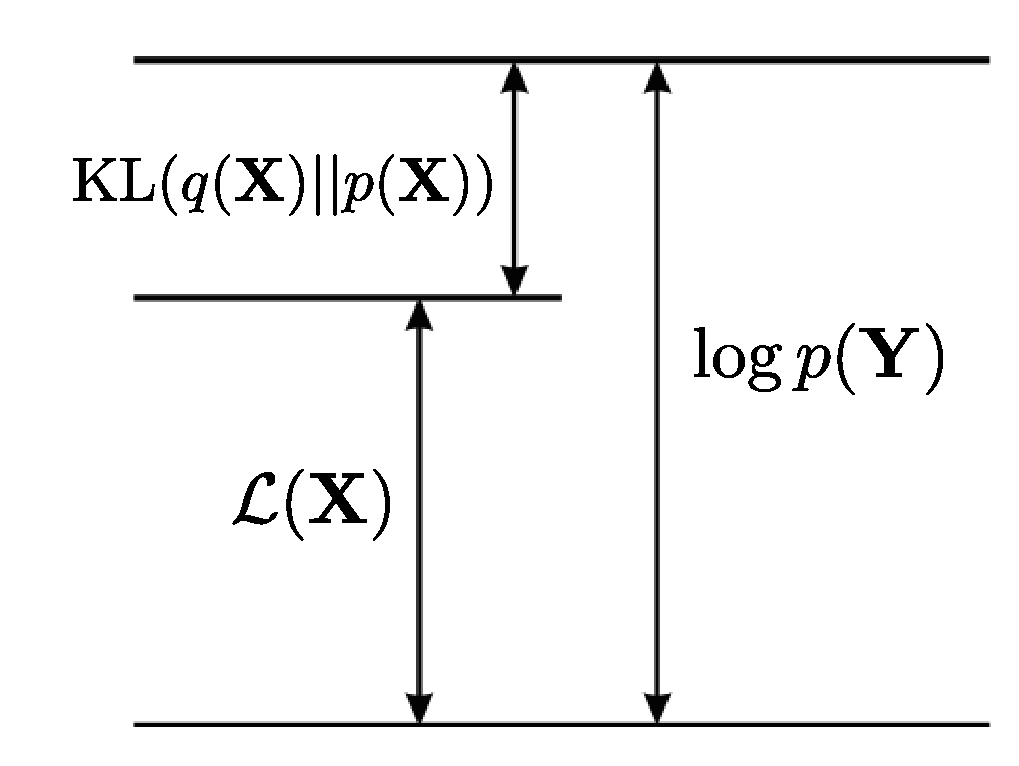
\includegraphics[width=0.35\linewidth]{lower_bound}
	\caption{The quantity $\Lagr(\bfX)$ provides a lower bound on the true log marginal likelihood $\log p(\bfY)$, with the difference being given by the Kullback-Leibler divergence $\KL(q||p)$ between the variational distribution $q(\bfX)$ and the true posterior $p(\bfX|\bfY)$}
	\label{fig:ELBO}
\end{figure}

There are several approaches to define $q(\bfX)$, the two most commonly used are called (unparametric) mean-field and (parametric) fixed-form \cite{Zhang2017,Blei2016}.

\subsubsection{Mean-field variational inference}  \label{section:mean_field}

The most common type of variational Bayes, known as the mean-field approach, assumes that the variational distribution factorises over M disjoint groups of unobserved variables\cite{Saul1996}:
\begin{equation} \label{eq:mean_field}
	q(\bfX) = \prod_{i=1}^{M} q(\bfx_i)
\end{equation}
where typically all unobserved variables are assumed to be independent. Importantly, notice that no parametric assumptions were placed regarding the nature of $q(\bfx_i)$.

Evidently, in sufficiently complex models where the unobserved variables have dependencies this family of distributions do not contain the true posterior (\Cref{fig:mean_field}). Yet, this is a key assumption to obtain an analytical inference scheme that yields surprisingly accurate results \cite{Blei2006,Faes2011,Braun2007}.

\begin{figure}[H]
	\centering
	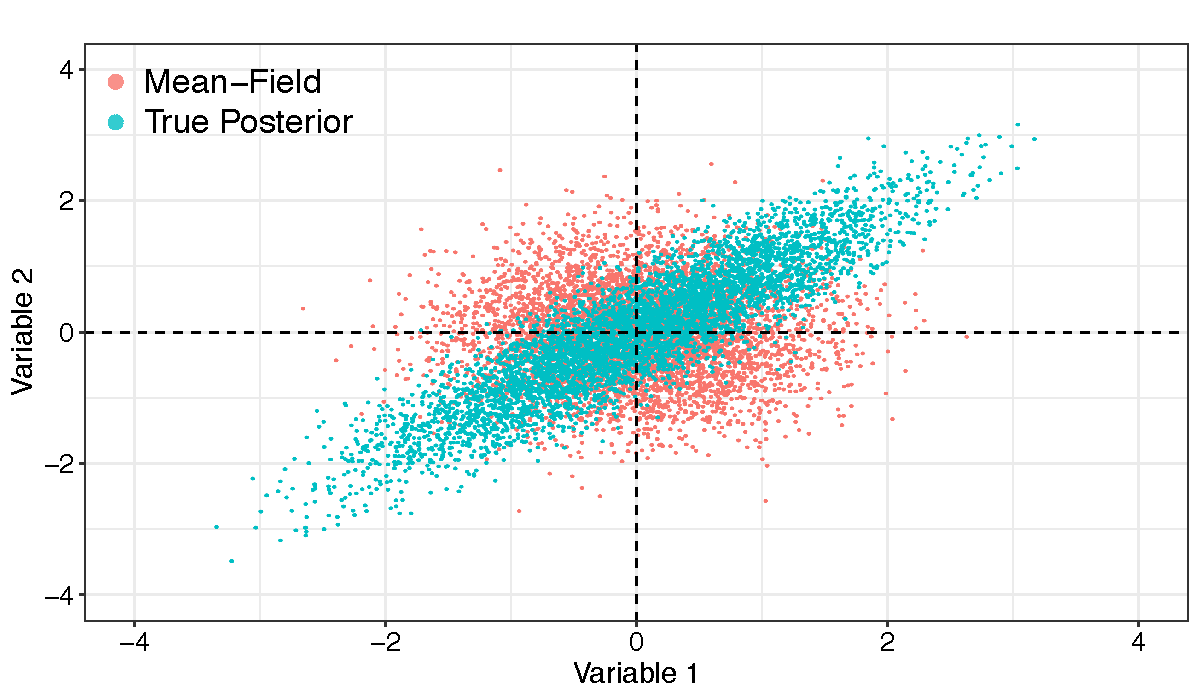
\includegraphics[width=0.7\linewidth]{mean_field}
	\caption{Illustrative example of sampling from a true posterior distribution (blue) versus a fitted mean-field varaitional distribution (red) in a model with two (correlated) unobserved variables. The mean-field approximation wrongly assumes that the unobserved variables are independent.}
	\label{fig:mean_field}
\end{figure}

Using calculus of variations (derivations can be found in \cite{Bishop,Murphy}), it follows that the optimal distribution $q(\bfX)$ that maximises the lower bound $\Lagr(\bfX)$ is
\begin{equation} \label{eq:optimal}
	\log \hat{q}_i(\bfx_i) = \E_{-i} [\log p(\bfY,\bfX)] + \mathrm{const}
\end{equation}
where $\E_{-i}$ denotes an expectation with respect to the $q$ distributions over all variables $\bfx_j$ except for $\bfx_i$.\\
The additive constant is set by normalising the distribution $\hat{q}_i(\bfz_i)$:
\[
	\hat{q}(\bfx_i) = \frac{\exp(\E_{-i}[\log p(\bfY,\bfX)])}{\int \exp(\E_{-i}[\log p(\bfY,\bfX)]) d\bfX}
\]
While the form of $\hat{q}(\bfx_i)$ is not restricted to a specific parametric form, it can be shown that when using conjugate priors, the distributions $\hat{q}_i(\bfx_i)$ have the same functional form as the priors $\hat{p}(\bfx_i)$. 
%An example is shown in Appendix X, but a detailed mathematical treatment with derivations of multiple examples can be found in \cite{Bishop,Murphy,Zhao2009}.


\subsubsection{Fixed-form variational inference}  \label{section:fixed_form}

An alternative and straightforward choice is to directly define a parametric form for the distribution $q(\bfX)$ with some parameters $\bTheta$. Once the choice of $q(\bfX)$ is made, the parameters $\bTheta$ are optimised to minimise $\KL(q(\bfX)||p(\bfX|\bfY))$ (the variational problem):
\begin{align}
	\hat{\bTheta} &= \argmin_{\bTheta} \KL(q(\bfX)||p(\bfX|\bfY)) \\
	&= \E[\log(q(\bfX)) - \log(p(\bfX,\bfY))]
\end{align}
Numerically optimising this function requires the evaluation of expectations with respect to $q(\bfX)$. In closed form, this is only feasable for a limited group of variational distributions. Alternatively, one can attempt Monte Carlo approximations, but in practice this turns to be slow and leads to high-variance estimates \cite{Braun2007,Ranganath2014,Braun2007}.

Typically, one would choose this distribution to factorise over parameters and to be of the same (exponential) family as the prior $p(\bfX)$. In such case there is a closed form coordinate-ascent scheme available, and it turns out that the fixed-form formulation is equivalent to the (non-parametric) mean-field derivation when using conjugate priors.\\
Unfortunately, for generic models with arbitrary families of distributions, no closed-form variational distributions exist \cite{Zhang2017,Blei2016}. 

However, while the parametric assumption certainly limits the flexibility of variational distributions, the advantage of this formulation is that it unveils the possibility to use fast gradient-based methods for the inference procedure \cite{Hoffman2012,Ranganath2014}.

%\paragraph{Black box variational inference}

\subsubsection{Expectation Propagation}  \label{section:expectation_propagation}

Expectation Propagation (EP) is another deterministic strategy with a similar philosophy as the Variational approach. It is also based on minimising the KL divergence between a variational distribution $q(\bfX)$ and the true posterior $p(\bfX|\bfY)$, but while variational inference minimises $KL(p||q)$, EP maximises the reverse KL-divergence $KL(q||p)$.

Interestingly, this simple difference leads to an inference scheme with stringkly different properties. This can be understood by inspecting the differences between the two KL divergence formulas:

Variational inference:
\begin{equation} \label{eq:kl_vb}
	\KL(q(\bfX)||p(\bfX|\bfY)) = - \int_z q(\bfX) \log \frac{p(\bfX|\bfY)}{q(\bfX)}
\end{equation}
Expectation propagation:
\begin{equation} \label{eq:kl_ep}
	\KL(p(\bfX|\bfY)||q(\bfX)) = - \int_z p(\bfX|\bfY) \log \frac{q(\bfX)}{p(\bfX|\bfY)}
\end{equation}
In regions of $\bfX$ where the true posterior density $p(\bfX|\bfY)$ is small, setting a large density for $q(\bfX)$ has a much stronger penalisation in \Cref{eq:kl_ep} than in \Cref{eq:kl_vb}, because of the true posterior density being on the denominator. Hence, EP tends to avoid areas where the density $p(\bfX|\bfY)$ is very low, even if it does not correspond to areas of very high-density in $p(\bfX|\bfY)$. In contrast, in \Cref{eq:kl_vb} there is a strong penalty for having low-density $q(\bfX)$ values.\\
As discussed in \cite{Bishop}, the practical consequences of this duality can be observed when the posterior is multi-modal, as in any sufficiently complex model. In VI, $q(\bfX)$ converges towards areas of high-density in $p(\bfX|\bfY)$, namely local optima. In contrast, EP tends to capture as much non-zero density regions from $p(\bfX|\bfY)$ as possible, thereby averaging across all optima. In the context of doing predictions, the VI solution is much more desirable than the EP solution, as the average of two good parameter values is not necessarily a good parameter itself.\\
A detailed mathematical treatment of EP, including derivations for specific examples, can be found in \cite{Bishop,Murphy,Minka2001}

\begin{figure}[H]
	\centering
	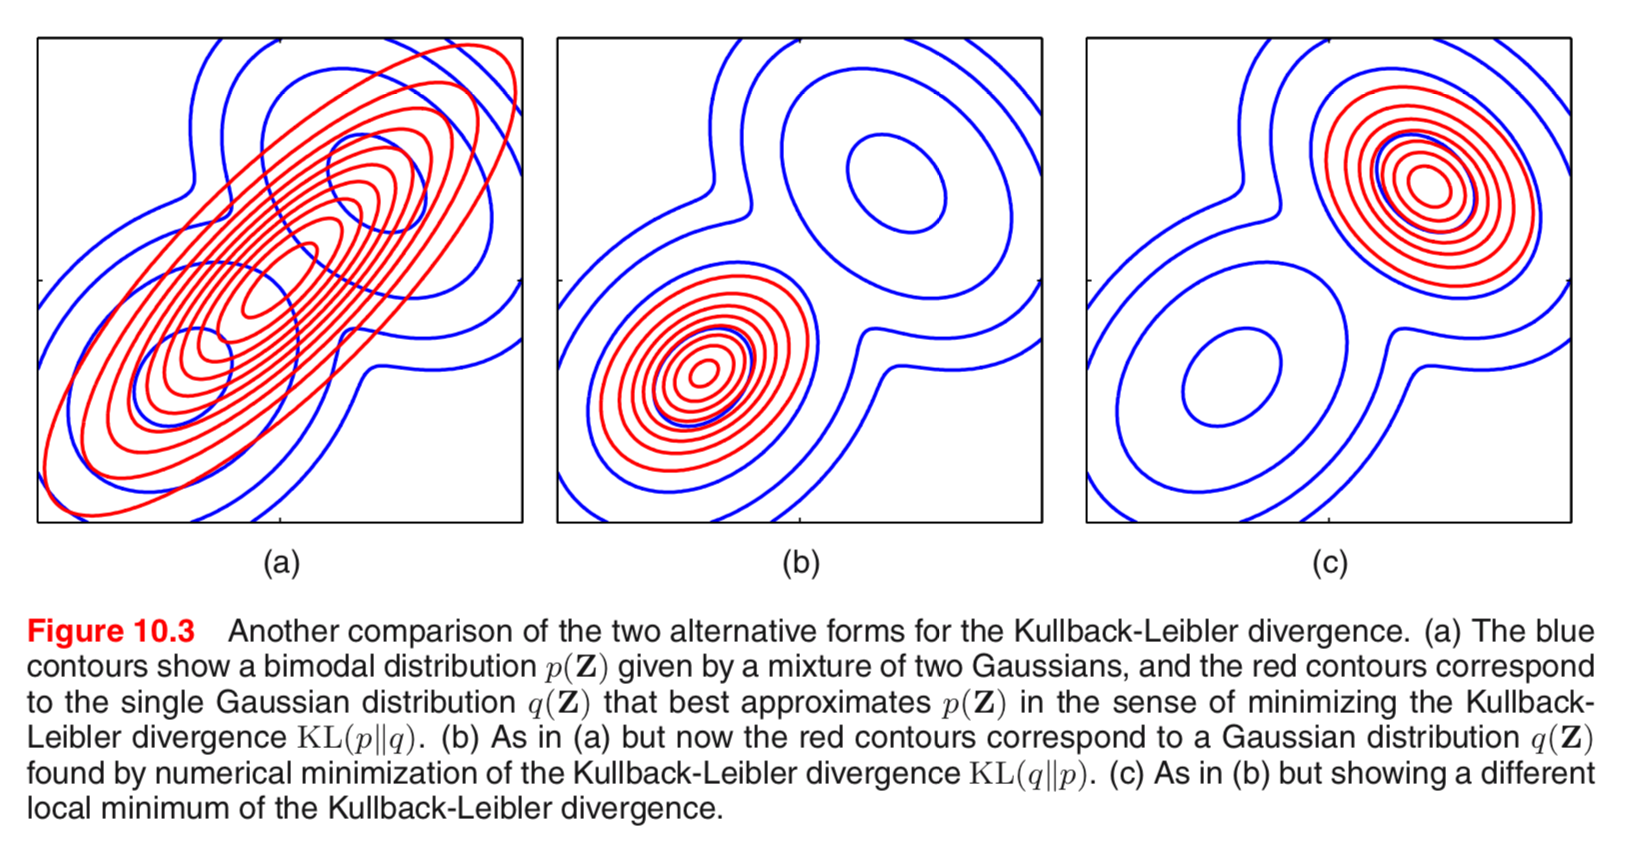
\includegraphics[width=1.0\linewidth]{VB_vs_EP}
	\caption{Illustrative comparison of Variational inference and Expectation Propagation. Shown is the (a) Density and (b) Variance of the true posterior distribution $p(\bfX|\bfY)$ (grey), the variational distribution (orange) and the expectation propagation distribution (green).}
	\label{}
\end{figure}

Following the rationale above, it is easy to predict that variational inference tends to be underestimate the variance of the posterior density. Yet, empirical research have shown that this is acceptable, provided that a good model selection is performed \cite{Blei2006}.


\subsubsection{Conclusions}

In this section we have introduced Bayesian modelling and variational inference methods, which will be used later in this chapter.\\
More generally, variational inference is growing in popularity for the analysis of big data sets and it has been applied to a myriad of different problems, including genome-wide association studies \cite{Carbonetto2012}, population genetics, \cite{Raj2014}, network analysis \cite{Sanguinetti2006} and natural language processing \cite{Blei2003}.

Yet, despite its increasing success, there is significant room for improvement. First and foremost, the theoretical guarantees of variational inference are not as developed as in sampling-based MCMC schemes\cite{Blei2016,Zhang2017,Nakajima2007}. As an example, the mean-field setting makes strong independence assumptions about the parameters.  Although it tends to besurprisingly effective, it is not clear in which applications the dependencies between the parameters are important enough than the mean-field approximation could potentially break.\\
More generally, an open research problem is understanding what are the statistical properties of the variational posterior with respect to the exact posterior \cite{Blei2016,Zhang2017}.

As we shall demonstrate later, alternative strategies have been considered to allow some dependencies between the variables, resulting in \textit{structured} mean-field approximations\cite{Hoffman2014,Titsias2011}. However, they often lead to very complex (if not intractable) inference frameworks. 

Finally, another area of extensive research is how to extend the applicability of VI to non-conjugate models. As discussed in \Cref{section:deterministic_bayesian_inference}, the ELBO of non-conjugate models contains intractable integrals, and setting up an inference scheme requires the use of either stochastic Monte Carlo approximations or deterministic approximations that introduce additional lower bounds \cite{Zhang2017,Seeger2012,Khan2017}. In this thesis we follow this rationale to derive an inference framework for a model with non-gaussian likelihoods.

%
\subsection{Latent variable models for genomics}

With the exponential growth in the use of high-throughput genomics, biological data sets are increasingly high dimensional, both in terms of samples and features. A key principle of biological data sets is that variation between the features results from differences in underlying, often unobserved, processes. Such processes, whether driven by biological or technical effects, are manifested by coordinated changes in multiple features. This key assumption sets off an entire statistical framework of exploiting the redundancy encoded in the data set to learn the (latent) sources of variation in an unsupervised fashion. This is the aim of dimensionality reduction techniques, or latent variable models \cite{Komili2008, Stegle2012, Leek2007, Pournara2007, Dai2017, Genevieve2018, Meng2016}.


\subsubsection{Mathematical formulation}

Given a dataset $\bfY$ of $N$ samples and $D$ features, latent variable models attempt to exploit the dependencies between the features by reducing the dimensionality of the data to a potentially small set of $K$ latent variables, also called factors. The mapping between the low-dimensional space and the high-dimensional space is performed via a function $f(\bfX|\bTheta)$ that depends on some parameters $\bTheta$.\\
The choice of $f(\bfX|\bTheta)$ is essentially the field of dimensionality reduction. A trade-off exists between complexity and interpretation: while non-linear functions such as deep neural networks provide more explanatory power, this leads to a considerable challenges in interpretation \cite{Zhang2018_NN}. Hence, for most applications where interpretability is essential, $f(\bfX|\bTheta)$ is assumed to be linear:
% \begin{equation} 
% 	y_{nd} = \sum_{k=1}^{K} w_{dk}z_{n,k}
% \end{equation}
\begin{equation} \label{eq:linear_model}
	\mathbf{Y} = \mathbf{Z}\mathbf{W}^{T}
\end{equation}
where $\bfZ \in \R^{N \times K}$ is a matrix that contains the low-dimensional representation for each sample (i.e. the factors). The matrix $\bfW \in \R^{D \times K}$ contains the weights, which provide the linear mapping between the features and the factors.\\
Note that the aim in dimensionality reduction is to exploit the coordinated heterogeneity between features, and hence features are assumed to be centered without loss of generality.

The inference procedure consists in learning the values of all unobserved variables, including factors and weights. As we shall demonstrate, different inference schemes and assumptions on the prior distributions lead to significantly different model outputs \cite{Rattray2009}.


\subsection{Principal Component Analysis} \label{section:pca}

Principal Component Analysis (PCA) is the most popular technique for dimensionality reduction \cite{Hotelling1933,Ringner2008}. Starting from \Cref{eq:linear_model}, two formulations of PCA exist \cite{Bishop2006}. In the maximum variance formulation, the aim is to infer an orthogonal projection of the data onto a low-dimensional space such that variance explained by the projected data is maximised. Formally, 

Formally, the aim in PCA is to infer the matrix $\bfW$ such that the variance of $\bfZ$ (the projected data) is maximised. If we consider a single latent factor, the variance of the projected data is:
\begin{equation*}
	\sigma^2 = \frac{1}{N}\sum_{n=1}^{N} (\bfz_n - \hat{\bfz})^{2} = \frac{1}{N}\sum_{n=1}^{N} (\bfy_n^T \bfw - \hat{\bfy}^T\bfw)^{2}
\end{equation*}

where $\hat{\bfy}$ is a vector with the feature-wise means. If we assumed centered data this simplifies to:
\begin{equation*}
	\sigma^2 = \frac{1}{N}\sum_{n=1}^{N} (\bfy_n^T \bfw)^{2}
\end{equation*}
Some algebra allows us to define this equation in terms of the (centered) data covariance matrix: $\bfS = \frac{1}{N}\sum_{n=1}^{N} \bfy_n\bfy_n^T$:
\begin{align*}
	\sigma^2 &= \frac{1}{N}\sum_{n=1}^{N} (\bfy_n^T \bfw)^T (\bfy_n^T \bfw) \\
	=& (\bfw^T \bfy_n) (\bfy_n^T \bfw) \\
	=& \bfw^T (\bfy_n \bfy_n^T) \bfw \\
	=& \bfw^T \bfS \bfw
\end{align*}

Thus, for a single principal component, the optimisation problem is:
\begin{equation} \label{eq:pca}
	%\argmax_{\|\bfw\|=1} & \sum_{n=1}^{N} (\bfw_1^T \bfy_n)^2 = \\
	\argmax_{\|\bfw\|=1} = \bfw^T \bfS \bfw
\end{equation}

% where $\bfY^T \bfY=\bfS \in \R^{D \times D}$ is the data covariance matrix and $\bfw_1^T$ is the vector of weights. \\
The $k$-th principal component can be found by subtracting from $\bfY$ the reconstructed data by the previous $k-1$ principal components. If we define $\bfz_k=\bfw_k^T \bfY$ to be the $k$-th principal component:
\[
	\hat{\bfY} = \bfY - \sum_{k=1}^{K} (\bfz_k \bfw_k^T)
\]
Re-applying \Cref{eq:pca} defines the new optimisation problem.

In its minimum error formulation, the aim is to find an equivalent projection that minimises the mean squared error between the observations and the data reconstructed using all principal components:
\[
	\argmax_{\|\bfw\|=1} \Vert \bfY - \sum_{k=1}^{K} (\bfz_k \bfw_k^T) \Vert^{2}
\]
where $\Vert \cdot \Vert^{2}$ is the Frobenius norm.

Remarkably, in both cases, solving the optimisation problems via Lagrange multipliers leads to master eigenvalue-eigenvector equation:
\begin{equation}
	\bfS \bfw_k = \lambda_k \bfw_k
\end{equation}
where the weight vectors $\bfw_k$ can be calculated as the eigenvectors of the covariance matrix $\bfS$ \cite{Bishop2006}.

Interestingly, the reason why the maximum variance solution and the minimum reconstruction error solution are the same can be understood by applying Pythagoras theorem to the right triangle defined by the projection of a sample $\bfy_{n}$ to a weight vector $\bfw$ (\Cref{fig:pca2}).
Assuming again centered data, the variance of $\bfy_{n}$ is $\|\bfy_{n}\| = \bfy_{n}^T \bfy_{n}$. This variance decomposes as the sum of the variance in the latent space $\|\bfz_{n}\| = \bfz_{n}^T \bfz_{n}$ and the residual variance after reconstruction $\|\bfy_{n} - \bfz_{n} \bfw^T \|$:

\begin{figure}[H]
	\centering
	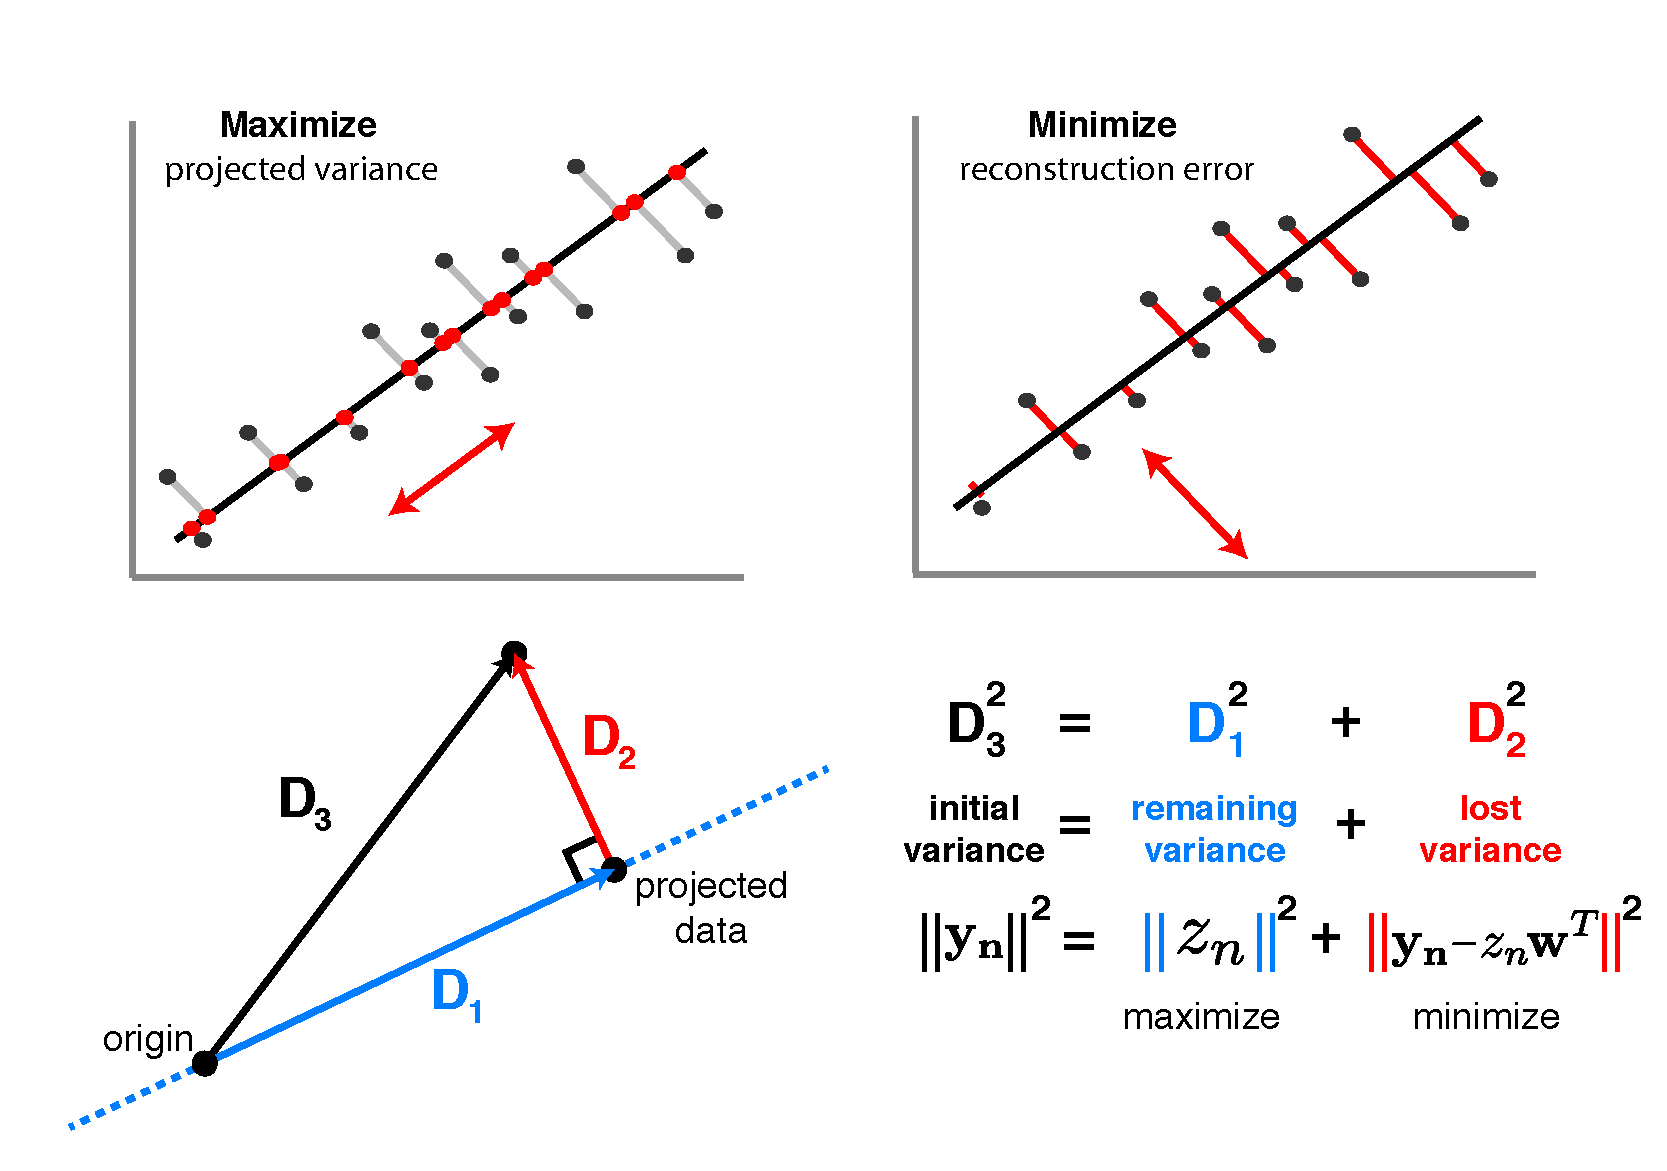
\includegraphics[width=0.8\linewidth]{pca2}
	\caption[Maximizing the variance in the principal component space is equivalent to minimizing the data reconstruction error]{In the maximum variance formulation the aim is to maximise the variance of the projected data (blue line), whereas in the minimum error formulation the aim is to minimise the residual variance (red line). Given a fixed total variance (black line), both strategies are equivalent}
	\label{fig:pca2}
\end{figure}

The main strength of PCA relies on its simplicity and closed form solution. Additionally, the linear mapping has the advantage of yielding interpretable feature weights, so that inspection of $\bfw_k$ reveals which features are jointly affected by the $k$-th principal component.\\
However, PCA suffers from serious drawbacks when applying it to real data sets \cite{Li2017b}. First, biological measurements are inherently noisy, and there is no explicit account of noise in PCA. In practice, high variance components are often asociated with signal whereas low-variance components are assumed to be noise, but an ideal model should explicitly disentangle the uncoordinated variability that is attributed to noise from the coordinated variability that is characterised as signal. Second, in its original formulation, no missing data is allowed \cite{Ilin2010}. Third, it does not offer a principled way of modelling prior information about the data.

\subsection{Probabilistic Principal Component Analysis and Factor Analysis} \label{section:probabilistic_pca}
A probabilistic version of PCA was initially proposed in \cite{Tipping1999}. It can be formulated by converting some (or all) fixed parameters into random variables and adding an explicit noise term to \Cref{eq:linear_model}:
\begin{equation}
	\bfY = \bfW \bfZ + \bepsilon
\end{equation}
where the weights $\bfW$ are assumed to be non-probabilistic parameters, but the noise $\bepsilon$ and the latent variables $\bfZ$ (the principal components) are assumed to follow an isotropic normal distribution:
\begin{align*}
	p(\bfZ) &= \prod_{n=1}^{N} \prod_{k=1}^{K} \Ndist{z_{nk}}{0,1} \\
	p(\epsilon) &= \Ndist {\epsilon}{0,\sigma^2}
\end{align*}
%The alternative strategy of treating $\bfZ$ as random variables and $\bfW$ as parameters has also been explored \cite{Lawrence2005}.\\

All together, this leads to a normally-distributed likelihood:
\begin{equation} \label{eq:ppca_lik}
	% p(\bfY|\bfW,\bfZ,\sigma) = \Ndist{\bfY}{\bfW \bfZ,\sigma^2 \I}
	p(\bfY|\bfW,\bfZ,\sigma) = \prod_{n=1}^{N} \prod_{d=1}^{D} \Ndist{y_{n,d}}{\bfw_{,:k}^T \bfz_{n,:},\sigma^2 \I}
\end{equation}

The corresponding graphical model is:

\begin{figure}[H]
	\centering
	% \definecolor{colD}{rgb}{0.2, 0.2, 0.6}
\definecolor{colM}{rgb}{0.0, 0.5, 0.0}
\definecolor{colN}{rgb}{0.5, 0.0, 0.13}
\definecolor{colG}{rgb}{1.0, 0.65, 0.0}
\newcommand\op{0.25}
\colorlet{shadecolor}{black!25}


\begin{tikzpicture}

% Define nodes
\node[obs]   (Y) {$y_{n,d}$};
\node[latent, xshift=-1.5cm, above=of Y, yshift=-0.4cm] (Z) {$z_{n,k}$};
\node[latent, double, double distance=1pt, above=of Y, yshift=0.6cm] (W) {$w_{d,k}$};
\node[latent, double, double distance=1pt, xshift=1.5cm] (Tau) {$\tau$};

% Connect the nodes
\edge {Z,W, Tau} {Y};

% Plates
\plate[] {plateK} {(Z)(W)} {$K$};
\plate[] {plateN} {(Y)(Z)(plateK.south east)(plateK.south west)} {$N$};
\plate[] {plateD} {(Y)(W)(plateK.north east)(plateN.south east)} {$D$};

\end{tikzpicture}
	\caption{Graphical model for probabilistic PCA. The latent variables are modelled as random variables, whereas the weights and the noise are modelled as deterministic parameters.}
	\label{fig:pPCA}
\end{figure}

Importantly, the choice of the distribution for $\epsilon$ implies that the noise of each feature is independent but restricted to have the same variance $\sigma^2$. In practice this is a limiting assumption, as different features are expected to show different degrees of noise, albeit this constraint can be relaxed and forms the basis of Factor Analysis \cite{Rubin1982,Bishop2006}.

The inference procedures involves learning the parameters $\bfW$, and $\sigma^2$ and a posterior probability distribution for $\bfZ$. As the model depends on latent variables, inference can be performed using the iterative Expectation-Maximisation (EM) algorithm \cite{Rubin1982,Bishop2006}. In the expectation step, the posterior distribution for $\bfZ$ is computed in closed form (due to conjugacy between the likelihood and the prior), given current estimates for the parameters $\bfW$, and $\sigma^2$. In the maximisation step, the parameters are calculated by maximising the expectation of the joint log likelihood under the posterior distribution of $\bfZ$ found in the E step \cite{Tipping1999}.\\
Interestingly, the EM solution of probabilistic PCA lies in the same subspace as the traditional PCA solution \cite{Tipping1999}, but the use of a probabilistic framework brings several benefits. First, model selection can be performed by comparing likelihoods across different settings of parameters. Second, missing data can naturally be accounted for by ignoring the missing observations from the likelihood. Finally, the probabilistic formulation sets the core framework for a Bayesian treatment of PCA, enabling a broad range of principled extensions tailored different types of data sets.


\subsection{Bayesian Principal Component Analysis and Bayesian Factor Analysis} \label{section:bayesian_pca}

The full Bayesian treatment of PCA requires the specification of prior probability distributions for all unobserved variables:
\begin{align*}
	p(\bfZ) &= \prod_{n=1}^{N} \prod_{k=1}^{K} \Ndist{z_{nk}}{0,1} \\
	p(\bfW) &= \prod_{d=1}^{D} \prod_{k=1}^{K} \Ndist{w_{dk}}{0,1} \\
	p(\epsilon) &= \Ndist {\epsilon}{0,\tau^{-1}} \\
	p(\tau) &= \Gdist{\tau}{a_0,b_0}
\end{align*}
where $\tau$ is the precision (inverse of the variance) of the noise term. A generalisation to Bayesian Factor Analysis follows by allowing a separate noise term per feature:
\begin{align*}
	p(\bepsilon) &= \prod_{d=1}^{D} \Ndist {\epsilon_d}{0,\tau_d^{-1}} \\
	p(\btau) &= \prod_{d=1}^{D} \Gdist{\tau_d}{a_0,b_0}
\end{align*}
where $a_0$ and $b_0$ are fixed hyperparameters. As in \Cref{eq:ppca_lik}, this results in a Normal likelihood:
\[
	p(\bfY|\bfW,\bfZ,\btau) = \prod_{n=1}^{N} \prod_{d=1}^{D} \Ndist{y_{nd}}{\bfw_{d}^T \bfz_{n},\tau_d}
\]

The corresponding graphical model is:

\begin{figure}[H] 
	\centering
	\begin{tikzpicture}

% Define nodes
\node[obs]   (Y) {$y_{n,d}$};
\node[latent, above=of Y, xshift=-1.5cm] (Z) {$z_{n,k}$};
\node[latent, above=of Y, xshift=1.5cm] (W) {$w_{d,k}$};
\node[latent, xshift=1.5cm] (Tau) {$\tau_{d}$};

% Connect the nodes
\edge {Z,W, Tau} {Y};

% Plates
\plate[] {plateK} {(Z)(W)} {$K$};
\plate[] {plateN} {(Y)(Z)(plateK.north west)} {$N$};
\plate[] {plateD} {(Y)(W)(Tau)(plateK.south east) (plateN.south east) (plateN.north east)} {$D$};

\end{tikzpicture}
	\caption{Graphical model for Bayesian Factor Analysis. All unobserved variables are modelled as random variables.}
	\label{fig:bayesianFA}
\end{figure}


\subsection{Hierarchical priors}  \label{section:hierarchical_priors}

A key advantage of the full Bayesian treatment is that it explicitly captures uncertainity on the estimation of all unobserved variables, as opposed to the probabilistic PCA model \cite{Bishop1999a,Bishop1999b}. Yet, more importantly, the use of (hierarchical) prior distributions allow different modelling assumptions to be encoded, providing a flexible and principled approach to extend PCA to a myriad of modelling scenarios, including multi-view generalisations \cite{Klami2008,Virtanen2012,Klami2015,Bunte2016,Khan2014,Zhao2016}.

\subsubsection{Automatic relevance determination} \label{section:ard}


As an example, a major challenge in PCA is how to determine the dimensionality of the latent space (i.e. the number of principal components). As we will show, the use of hierarchical prior distributions allows the model to introduce sparsity assumptions on the weights in such a way that the model automatically learns the number of factors.\\
In the context of Factor Analysis, one the first sparsity priors to be proposed was the Automatic Relevance determination (ARD) prior \cite{Neal1995,Mackay1996,Bishop1999a,Bishop1999b}. 
\begin{equation*} \label{eq:ard}
	p(\bfW|\balpha) = \prod_{k=1}^{K} \Ndist{\bfw_{:,k}}{0,\frac{1}{\alpha_{k}}\I_{D}} \\
	\qquad\qquad
	p(\balpha) = \prod_{k=1}^{K} \Gdist{\alpha_k}{a_0^\alpha, b_0^\alpha}
\end{equation*}
The aim of this prior is two-fold. First, the zero-mean normal distribution specifies that, \textit{a priori}, no information is available and all features are \textit{inactive}. When exposed to some data, the posterior distribution for $\bfW$ will be estimated by weighting the contribution from the likelihood, potentially allowing features to escape from the zero-centered prior (\Cref{fig:ard}).\\
Second, performing inference on the variable $\balpha = \{ \alpha_1, \cdots, \alpha_k \}$ enables the model to discard inactive factors. To understand this, let us assume that only $K=5$ true factors exist, but the model is initialised with $K=20$ factors. In such case, inactive factors can be prunned out by driving the corresponding $\alpha_k$ to infinity. In turn, this causes the posterior $p(\bfw_{:,k}|\bfY)$ to be sharply peaked at zero, resulting in the inactivation of all its weights. %\Cref{fig:hinton}.

\begin{figure}[H] \begin{center}
	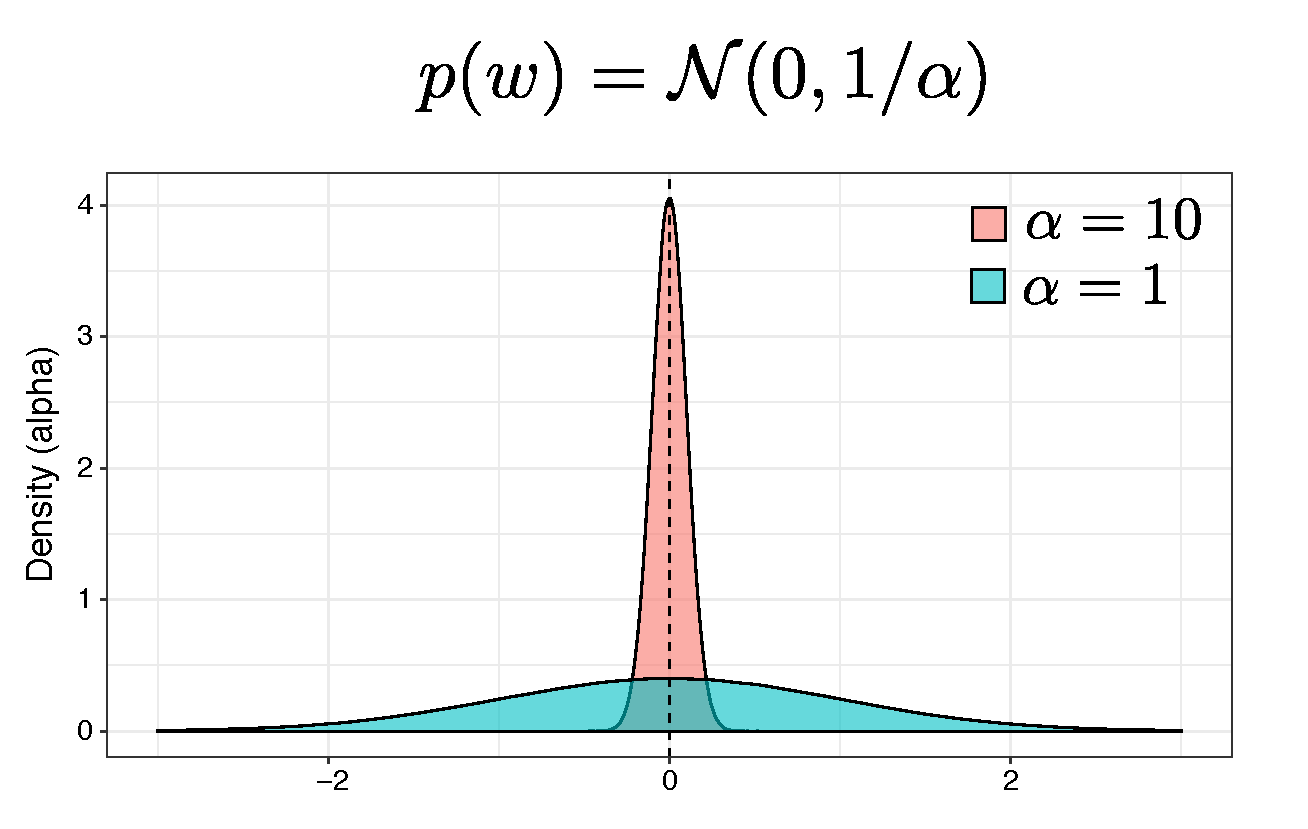
\includegraphics[width=0.7\textwidth]{Chapter2/Figs/ard}
	\caption{Visualisation of the sparsity-inducing Automatic Relevance Determination prior}
	\label{fig:ard}
\end{center} \end{figure}

% \begin{figure}[H] \begin{center}
% 	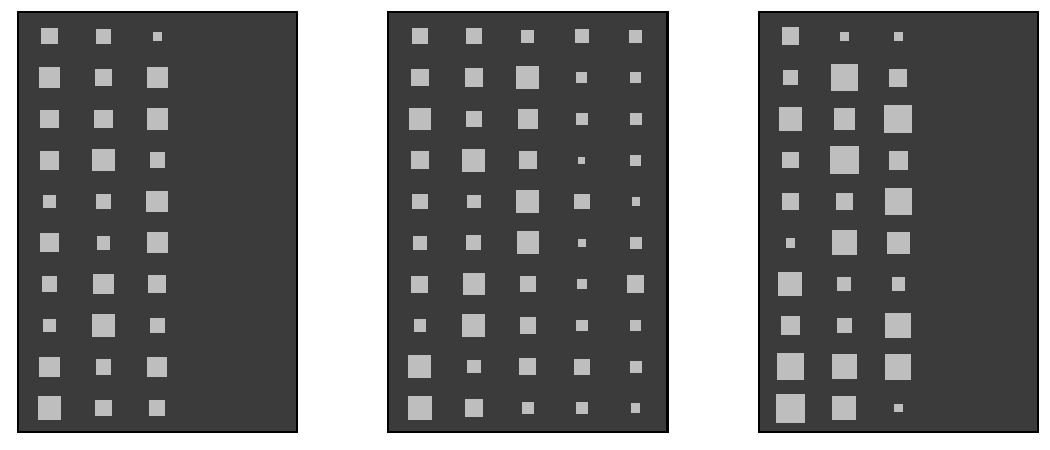
\includegraphics[width=0.8\textwidth]{Chapter2/Figs/hinton}
%             \caption[Hinton plot of the weight matrix for a Bayesian Factor Analysis model with an ARD prior]{Hinton plots display the values of the weight matrix, similar to a heatmap, where bigger squares depict larger weights. Shown are the Hinton plots for (a) the true weights, (b) the infered weights by a Factor Analysis model with no ARD prior (middle), and (c) the infered weights by a Factor Analysis model with ARD prior per factor. This figure was generated using simulated data with $N=100$ samples, $D=10$ features and $K=3$ factors.}
% 	\label{fig:hinton}
% \end{center} \end{figure}

\subsubsection{Spike-and-slab prior} \label{section_spikeslab}

Sparse extensions of the Bayesian factor analysis model have been proposed as a regularisation mechanism but also to model inherent assumptions regarding the sparse nature of biological data \cite{Stegle2012,Gao2013}.\\
The variability observed in biological data is driven both by technical factors and biological factors. Technical factors (i.e. batch effects) tend to be relatively strong and alter the expression of a large proportion of genes, whereas the biological factors are potentially weak effects driven by changes in small gene regulatory networks \cite{Gao2013}. Hence, a practical factor analysis model should be able to learn factors with different degrees of sparsity.\\
The ARD prior proposed in \Cref{eq:ard} allows entire factors to be dropped out from the model, but it provides a weak degree of regularisation when it comes to inactivating individual weights within the active factors.

A sparse generalisation of the Factor Analysis model proposed above can be achieved by combining the ARD prior with a spike-and-slab prior \cite{Mitchell1988,Titsias2011}:
\begin{align}
	p(w_{d,k} \mid \alpha_k,\theta_k) &= (1-\theta_k) \mathds{1}_0(w_{d,k}) + \theta_k \Ndist{w_{d,k}}{0, \alpha_k^{-1}} \\
	p(\theta_k) &= \Bdist{\theta_k}{a_0^\theta,b_0^\theta} \\
	p(\alpha_k) &= \Gdist{\alpha_k}{a_0^\alpha, b_0^\alpha}
\end{align}

The corresponding graphical model is:

\begin{figure}[H] \begin{center}
	\begin{tikzpicture}

% Define nodes
\node[obs]   (Y) {$y_{n,d}$};
\node[latent, above=of Y, xshift=-1.5cm] (Z) {$z_{n,k}$};
\node[latent, above=of W, xshift=-0.75cm] (Theta) {$\theta_{k}$};
\node[latent, above=of W, xshift=0.75cm] (Alpha) {$\alpha_{k}$};
\node[latent, above=of Y, xshift=1.5cm] (W) {$w_{d,k}$};
\node[latent, xshift=1.5cm] (Tau) {$\tau_{d}$};

% Connect the nodes
\edge {Theta, Alpha} {W};
\edge {Z, W, Tau} {Y};

% Plates
\plate[] {plateK} {(Z)(W)(Theta)(Alpha)} {$K$};
% \plate[] {plateN} {(Y)(Z)(plateK.north west)} {$N$};
\plate[] {plateN} {(Y)(Z)} {$N$};
\plate[] {plateD} {(Y)(W)(Tau)(plateK.south east) (plateN.south east) (plateN.north east)} {$D$};

\end{tikzpicture}
	\label{fig:bayesianFA}
	\caption{Graphical model for Bayesian sparse Factor Analysis. A double sparsity-inducing prior is used on the weights: an ARD prior to prune inactive factors and a spike-and-slab prior to inactive individual features within the active factors.}
\end{center} \end{figure}

The spike-and-slab prior is effectively a mixture model where features are sampled from a zero-inflated Gaussian distribution, where $\theta_k \in (0,1)$ dictates the level of sparsity per factor (i.e. how many active features). A value of $\theta_k$ close to $0$ implies that most of the weights of factor $k$ are shrunk to $0$ (i.e. a sparse factor), whereas a value of $\theta_k$ close to $1$ implies that most of the weights are non-zero (i.e. dense factors). By learning $\theta_k$ from the data, the model naturally accounts for combinations of sparse and dense factors.


% \subsubsection{Inference}
% In a fully Bayesian setting, the inference procedure corresponds to learning the posterior distributions for each unobserved variable. However, applying Bayes rule yields an analytically intractable solution, and approximate methods are required. This is discussed in Chapter X.



\subsection{Multi-view factor analysis models}

Probabilistic PCA and Factor Analysis perform dimensionality reduction from a single input matrix. In some occasions data is collected from multiple data sources that exibit heterogeneous statistical properties, resulting in a structured data set where features are naturally partitioned into views \cite{Xu2013,Li2016,Zeng2018}. A clear biological example is multi-omics data, where, for the same set of samples, multiple molecular layers are profiled. Each of the data modalities can be analysed separately using conventional (single-view) methods, but in the ideal strategy a single model should be used to leverage information across all molecular layers using a flexible and principled approach. This is referred to as the multi-view learning problem \cite{Xu2013,Li2016}.\\
A tempting approach to circumvent the multi-view learning problem is to simply concatenate all data sets before applying conventional (single-view) latent variable models \cite{Ritchie2015}. However, this is prone to fail for several reasons. First, heterogeneous data modalities cannot always be modelled using the same likelihood function. For example, continuous measurements are often modelled using a normal distribution, but binary and count-based traits are not appropriately modelled by this distribution \cite{Pilling2018}. Second, even if all views are modelled with the same likelihood, differences in the scale and the magnitude of the variance can lead to some views being overrepresented in the latent space. Finally, in a multi-view data set we expect multiple sources of variation, some driven by a single view, whereas others could capture shared variability across multiple views. In other words, from a structured input space, one can also expect a structured latent representation. Not taking this behaviour into account can lead to challenges in the interpretability of the latent space.

A comprehensive review of multi-view machine learning methods can be found in \cite{Xu2013} and a more genomics-oriented perspective in \cite{Ritchie2015}. For the purpose of this thesis, I will describe only the use of latent variable models for multi-view data integration.

\subsection{Canonical Correlation Analysis} \label{cca}

Canonical Correlation Analysis (CCA) is a simple extension of PCA to find linear components that capture correlations between two datasets \cite{Hotteling1936,Hardle2007}.\\
Given two data matrices $\bfY_1 \in \R^{N \times D_1}$ and $\bfY_2 \in \R^{N \times D_2}$ CCA finds a set of linear combinations $\bfU \in \R^{D_1 \times K}$ and $\bfV \in \R^{D_2 \times K}$ with maximal cross-correlation.
For the first pair of canonical variables, the optimisation problem is:
\[
	(\hat{\bfu_1}, \hat{\bfv_1}) = \argmax_{\bfu_1,\bfv_1} corr(\bfu_{1}^T \bfY_1, \bfv_{1}^T \bfY_2)
\]
As in conventional PCA, the linear components are constraint to be orthogonal. Hence, the first pair of canonical variables $\bfu_1$ and $\bfv_1$ contain the linear combination of variables that have maximal correlation. Subsequently, the second pair of canonical variables $\bfu_2$ and $\bfv_2$ is found from the residuals of the first canonical variables.

Given the similarity with PCA, both methods share statistical properties, including the linear mapping between the low-dimensional space and the high-dimensional space, and the closed-form solution using singular value decomposition \cite{Hotteling1936,Hardle2007}.\\
Because of its simplicity and efficient computation, CCA has widespread use as a dimensionality reduction technique \cite{Hardle2007}. Yet, as expected, CCA suffers from the same pitfalls as PCA: difficulties in selecting the number of components, lack of sparsity in the solutions and absence of probabilistic formulation. In addition, CCA have been shown to overfit for datasets where $D>>N$ \cite{McCabe2018,Guo2016}. Hence, probabilistic versions with sparsity assumptions that reduce overfitting and improve interpretability followed.


\subsubsection{Probabilistic Canonical Correlation Analysis} \label{section_probabilisticCCA}

Following the derivation of probabilistic PCA \cite{Tipping1999}, a similar effort enabled a probabilistic formulation of CCA as a generative model \cite{Bach2005}.\\
In this model, the two matrix of observations $\bfY^{1}$ and $\bfY^{2}$ are decomposed in terms of two weight matrices $\bfW^{1}$ and $\bfW^{2}$ but a joint latent matrix $\bfZ$:
\begin{align*}
	\bfY^{1} &= \bfW^{1} \bfZ + \epsilon^{1} \\
	\bfY^{2} &= \bfW^{2} \bfZ + \epsilon^{2}
\end{align*}
With the following prior probability distributions:
\begin{align*}
	p(z_{nk}) &= \Ndist{z_{nk}}{0,1} \\
	p(\epsilon^{1}) &= \Ndist {\epsilon^{1}}{\tau_{1}^{-1}} \\
	p(\epsilon^{2}) &= \Ndist {\epsilon^{2}}{\tau_{2}^{-1}}
\end{align*}
As in \cite{Tipping1999}, the weights and the variance of the noise are assumed to be non-probabilistic parameters, whereas the factors are probabilistic unobserved variables. This yields the following likelihood functions:
\begin{align} \label{eq:probabilistic_cca_likelihood}
	p(\bfY^{1}|\bfW^{1},\bfZ,\tau_{1}) &= \prod_{n=1}^{N} \prod_{d=1}^{D_1} \Ndist{y^{1}_{n,d}}{(\bfw_{:,k}^{1})^T \bfz_{n},\tau_{1}^{-1}} \\
	p(\bfY^{2}|\bfW^{2},\bfZ,\tau_{2}) &= \prod_{n=1}^{N} \prod_{d=1}^{D_2} \Ndist{y^{2}_{n,d}}{(\bfw_{:,k}^{2})^T \bfz_{n},\tau_{2}^{-1}} \nonumber
\end{align}

The corresponding graphical model is:
\begin{figure}[H] \begin{center}
	\begin{tikzpicture}

% Define nodes
\node[obs, xshift=-1.5cm] (Y1) {$y^{1}_{n,d}$};
\node[obs, xshift=+1.5cm] (Y2) {$y^{2}_{n,d}$};

\node[latent, below=of Y1, yshift=+0.5cm, xshift=+1.5cm] (Z) {$z_{n,k}$};

\node[latent, double, double distance=1pt, below=of Y1, xshift=-1cm, yshift=-1cm] (W1) {$w^{1}_{d,k}$};
\node[latent, double, double distance=1pt, below=of Y2, xshift=+1cm, yshift=-1cm] (W2) {$w^{2}_{d,k}$};

\node[latent, double, double distance=1pt, left=of Y1, yshift=-0.5cm] (Tau1) {$\tau^{1}$};
\node[latent, double, double distance=1pt, right=of Y2, yshift=-0.5cm] (Tau2) {$\tau^{2}$};

% Connect the nodes
\edge {Z} {Y1};
\edge {Z} {Y2};
\edge {W1} {Y1};
\edge {W2} {Y2};
\edge {Tau1} {Y1};
\edge {Tau2} {Y2};
% \edge {Z,W, Tau} {Y};

% Plates
\plate[] {plateK} {(Z)(W1)(W2)} {$K$};
% \plate[] {plateN} {(Y1)(Y2)(Z)(plateD1.north)} {$N$};
% \plate[] {plateD1} {(Y1)(W1)(plateK.south)(plateN.north)} {$D_1$};
% \plate[] {plateD2} {(Y2)(W2)(plateK.south)(plateN.north)} {$D_2$};
\plate[] {plateN} {(Y1)(Y2)(Z)} {$N$};
\plate[] {plateD1} {(Y1)(W1)(Tau1)} {$D_1$};
\plate[] {plateD2} {(Y2)(W2)(Tau2)} {$D_2$};

\end{tikzpicture}



	\label{fig:graphical_CCA}
	\caption{Graphical model for probabilistic Canonical Correlation Analysis}
\end{center} \end{figure}

Notice that the observations for both data sets are generated from the same set of latent variables $\bfZ$. This ensures that the model is focused on capturing the variation associated with cross-correlated groups of features.

Analogously to probabilistic PCA, the expected value of the posterior distribution $p(\bfZ|\bfY^{1},\bfY^{2})$ span the same subspace as standard CCA \cite{Bach2005}. Nonetheless, one of the many advantage of a probabilistic formulation is that it enables a broad range of principled extensions into larger graphical models.


\subsubsection{Bayesian Canonical Correlation Analysis} \label{section:bayesian_cca}

A fully Bayesian treatment of CCA followed based on exactly the same principle presented in \Cref{section:bayesian_pca} by introducing prior distributions to all unobserved variables \cite{Wang2007,Klami2013}:
\begin{align*} 
	p(\bfZ) &= \prod_{n=1}^{N} \prod_{k=1}^{K} \Ndist{z_{nk}}{0,1} \\
	p(\epsilon^{1}) &= \Ndist {\epsilon^{1}}{\sigma_{1}^{2}} \\
	p(\epsilon^{2}) &= \Ndist {\epsilon^{2}}{\sigma_{2}^{2}} \\
	p(\bfW^1|\balpha) &= \prod_{k=1}^{K} \Ndist{\bfw^{1}_{:,k}}{0,\frac{1}{\alpha_{k}}\I_{D_1}} \\
	p(\bfW^2|\balpha) &= \prod_{k=1}^{K} \Ndist{\bfw^{2}_{:,k}}{0,\frac{1}{\alpha_{k}}\I_{D_2}} \\
	p(\balpha) &= \prod_{k=1}^{K} \Gdist{\alpha_k}{a_0^\alpha, b_0^\alpha}
\end{align*}
Resulting in the same likelihood model as in \Cref{eq:probabilistic_cca_likelihood}. Yet, notice that an ARD is introduced per factor, allowing an automatic inference of the dimensionality in the latent subspace.
Also, there is some flexibility in the definition of noise. Whereas an independent noise term can be defined per view, one can also model correlated noise by introducing a multivariate Gaussian distribution with full-rank covariance \cite{Wang2007,Klami2013}.

The corresponding graphical model is:
\begin{figure}[H] \begin{center}
	\begin{tikzpicture}

% Define nodes
\node[obs, xshift=-1.5cm] (Y1) {$y^{1}_{n,d}$};
\node[obs, xshift=+1.5cm] (Y2) {$y^{2}_{n,d}$};

\node[latent, below=of Y1, yshift=+0.5cm, xshift=+1.5cm] (Z) {$z_{n,k}$};

\node[latent, below=of Y1, xshift=-1cm, yshift=-1cm] (W1) {$w^{1}_{d,k}$};
\node[latent, below=of Y2, xshift=+1cm, yshift=-1cm] (W2) {$w^{2}_{d,k}$};

\node[latent, left=of Y1, yshift=-0.5cm] (Tau1) {$\tau^{1}$};
\node[latent, right=of Y2, yshift=-0.5cm] (Tau2) {$\tau^{2}$};

% Connect the nodes
\edge {Z} {Y1};
\edge {Z} {Y2};
\edge {W1} {Y1};
\edge {W2} {Y2};
\edge {Tau1} {Y1};
\edge {Tau2} {Y2};
% \edge {Z,W, Tau} {Y};

% Plates
\plate[] {plateK} {(Z)(W1)(W2)} {$K$};
% \plate[] {plateN} {(Y1)(Y2)(Z)(plateD1.north)} {$N$};
% \plate[] {plateD1} {(Y1)(W1)(plateK.south)(plateN.north)} {$D_1$};
% \plate[] {plateD2} {(Y2)(W2)(plateK.south)(plateN.north)} {$D_2$};
\plate[] {plateN} {(Y1)(Y2)(Z)} {$N$};
\plate[] {plateD1} {(Y1)(W1)(Tau1)} {$D_1$};
\plate[] {plateD2} {(Y2)(W2)(Tau2)} {$D_2$};

\end{tikzpicture}
	\label{fig:graphical_bayesianCCA}
	\caption{Graphical model for Bayesian Canonical Correlation Analysis}
\end{center} \end{figure}

As expected, the sparsity priors yield a more sparse solution than traditional CCA, which is more appropriate for biological data analysis. However, this solution is still limited to $M=2$ views, which leads us to the next model extension.

% (\Cref{fig:hinton_cca}):
% \begin{figure}[H]
% 	\centering
% 	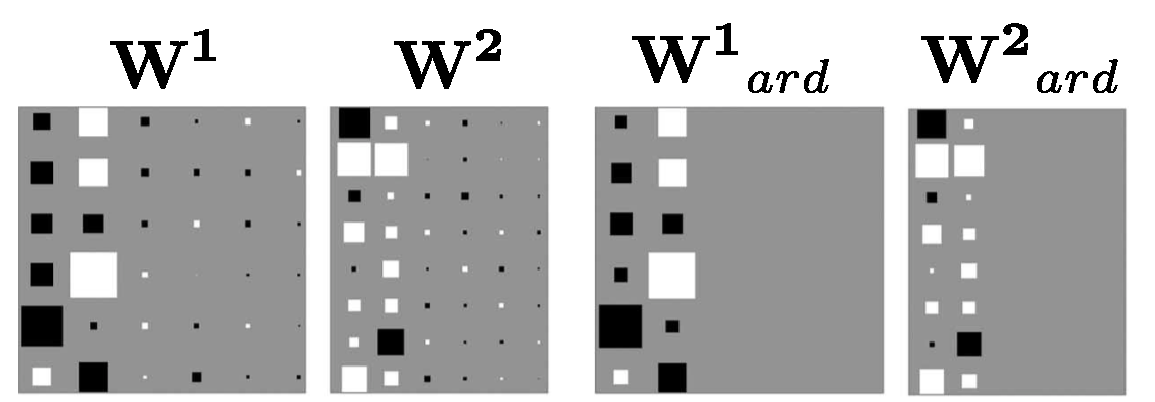
\includegraphics[width=0.85\linewidth]{hinton_cca}
% 	\caption{Comparison of the Hinton's diagram of $\bfW^{1}$ and $\bfW^{2}$ for the maximum likelihood CCA model (two left plots) and the variational Bayes CCA model (two right plots). Reprinted from \cite{Wang2007} with modifications.}
% 	\label{fig:hinton_cca}
% \end{figure}


\subsection{Group Factor Analysis} \label{section:gfa}

Group Factor Analysis (GFA) is the natural generalisation of Bayesian Canonical Correlation Analysis to an arbitrary number of views.
The original idea was originally presented in \cite{Virtanen2012} and a series of generalisations followed, tailored with specific assumptions for different applications \cite{Klami2015,Leppaaho2017,Bunte2016,Khan2014,Zhao2016,Remes2015}. In this section we will outline the core principle of GFA.

Given a data set of $M$ views $\bfY_1, \cdots, \bfY_M$, the task of GFA is to find $K$ factors that capture the variability \textit{within} as well as the variability \textit{between} views. In other words, we want to capture factors that not only explain variance that is shared across all views but we also want to capture factors that explain variance within a single view or between different subsets of views.\\
The starting point is to generalise the Bayesian CCA model (\Cref{section:bayesian_cca}) to $M$ views:
\begin{align*}
	\bfY^{1} &= \bfW^{2} \bfZ + \epsilon^{1} \\
	\bfY^{2} &= \bfW^{2} \bfZ + \epsilon^{2} \\
	& \cdots \\
	\bfY^{M} &= \bfW^{M} \bfZ + \epsilon^{M}
\end{align*}
Notice that there is a common factor space for all views, but there is a view-specific weight matrix. The key to disentangle the activity of each factor in each view lies on the sparsity structure imposed in the weights. Intuitively, if a factor $k$ is not driving any variation in a specific view $m$ we want all the individual weights to be pushed to zero. As shown before, this behaviour can be achieved using Automatic Relevance Determination (ARD) priors. However, if we were to use the same approach as in Bayesian CCA, where the ARD prior for factor $k$ is shared across all views, then factors would be restricted to have the same activity across all views.\\
In GFA this is generalised as follows:
\begin{align}
	p(\bfW) &= \prod_{m=1}^{M} \prod_{k=1}^{K} \Ndist{\bfw_{:,k}^m}{0,\frac{1}{\alpha_k^m}} \\
	p(\balpha) &= \prod_{m=1}^{M} \prod_{k=1}^{K} \Gdist{\alpha_k^m}{a_0^\alpha, b_0^\alpha}
\end{align}
This is effectively setting an ARD prior per factor $k$ and view $m$. The matrix $\balpha \in \R^{M \times K}$ defines four types of factors: (1) Inactive factors that do not explain variance in any view, which corresponds to all values $\balpha_k$ being large. (2) Fully shared factors that explain variance across all views, which corresponds to all values $\balpha_k$ being small. (3) Unique factors that explain variance in a single view, which corresponds to all values $\balpha_k$ being large, except for one entry. (4) Partially shared factors that explain variance in a subsets views, which corresponds to a mixture of small and large values for $\balpha_k$.\\

The corresponding graphical model is:

\begin{figure}[H] \begin{center}
	% \begin{tikzpicture}

% % Define nodes
% \node[obs, xshift=-1.5cm] (Y1) {$y^{m}_{n,d}$};

% \node[latent, below=of Y1, yshift=+0.5cm, xshift=+1.5cm] (Z) {$z_{n,k}$};

% \node[latent, double, double distance=1pt, below=of Y1, xshift=-1cm, yshift=-1cm] (W1) {$w^{1}_{d,k}$};
% \node[latent, double, double distance=1pt, below=of Y2, xshift=+1cm, yshift=-1cm] (W2) {$w^{2}_{d,k}$};

% \node[latent, double, double distance=1pt, left=of Y1, yshift=-0.5cm] (Tau1) {$\tau^{1}$};
% \node[latent, double, double distance=1pt, right=of Y2, yshift=-0.5cm] (Tau2) {$\tau^{2}$};

% % Connect the nodes
% \edge {Z} {Y1};
% \edge {Z} {Y2};
% \edge {W1} {Y1};
% \edge {W2} {Y2};
% \edge {Tau1} {Y1};
% \edge {Tau2} {Y2};
% % \edge {Z,W, Tau} {Y};

% % Plates
% \plate[] {plateK} {(Z)(W1)(W2)} {$K$};
% % \plate[] {plateN} {(Y1)(Y2)(Z)(plateD1.north)} {$N$};
% % \plate[] {plateD1} {(Y1)(W1)(plateK.south)(plateN.north)} {$D_1$};
% % \plate[] {plateD2} {(Y2)(W2)(plateK.south)(plateN.north)} {$D_2$};
% \plate[] {plateN} {(Y1)(Y2)(Z)} {$N$};
% \plate[] {plateD1} {(Y1)(W1)(Tau1)} {$D_1$};
% \plate[] {plateD2} {(Y2)(W2)(Tau2)} {$D_2$};

% \end{tikzpicture}



\begin{tikzpicture}
  % Define nodes:
  % matrix factorisation level
  \node[obs]   (Y) {$y_{n,d}^m$};
  \node[latent, above=of Y, xshift=-1.5cm] (Z) {$z_{n,k}$};
  \node[latent, above=of Y, xshift=1.5cm] (W) {$w^m_{k,d}$};
  % \node[latent, xshift=1.5cm] (Tau) {$\tau^m_{d}$};
  \node[latent, xshift=2.5cm] (Tau) {$\tau^m$};
  \node[latent, above=of W] (alpha) {$\alpha^m_{k}$};

  % Connect the nodes
  \edge {Z,W,Tau} {Y}; %
  \edge {alpha} {W};

  % Plates
  \plate[] {plateK} {(Z)(W)(alpha)} {$K$};
  \plate[] {plateN} {(Y)(Z) (plateK.south west)} {$N$};
  % \plate[] {plateD} {(Y)(W) (plateK.south east) (plateN.south east) (plateN.north east)} {$D_m$};
  \plate[] {plateD} {(Y)(W)} {$D_m$};
  % \plate[] {plateM} {(Tau) (plateK.north east)(plateD.south east)(plateD.south west)} {$M$};
  \plate[] {plateM} {(Y)(W)(Tau)(alpha)} {$M$};
\end{tikzpicture}

	\label{fig:graphical_GFA}
	\caption{Graphical model for Bayesian Group Factor Analysis}
\end{center} \end{figure}


Finally, notice that if $M=1$ the model reduces to Bayesian PCA (\Cref{section:bayesian_pca}), but when $M=2$ the model does \textit{not} reduce to Bayesian CCA because in the GFA setting factors are also allowed to capture both inter-specific variability (i.e. across views) and intra-specific variability (within a view). In Bayesian CCA, the views share a common ARD prior per factor to enforce the factors to explain variation in both views, at the expense of ignoring sources of variability that are specific to a single view.

%\graphicspath{{Chapter2/Figs/}}

\section{Multi-Omics Factor Analysis: a framework for unsupervised integration of multi-omics data sets}
% In the first section of this chapter, we will describe XXX

The work described in this chapter results from a collaboration with the Multi-omics and statistical computing group lead by Wolfgang Huber at the EMBL (Heidelberg, Germany). It has been peer-reviewed and published in \cite{Argelaguet2018}.\\

The method was conceived by Florian Buettner, Oliver Stegle and me. I performed most of the mathematical derivations and implementation, but with significant contributions from Damien Arnol and Britta Velten. The single-cell application was led by me whereas the CLL data application was led by Britta Velten, but with joint contributions in either cases. Florian Buettner, Wolfgang Huber and Oliver Stegle supervised the project.\\
The article was jointly written by Britta Velten, Florian Buettner, Wolfgang Huber, Oliver Stegle and me.


\subsection{Model description} \label{mofa:model_description}
MOFA is a multi-view generalisation of traditional Factor Analysis to $M$ input matrices (or views) $\bfY^m \in \R^{N \times D_m}$ based on the framework of Group Factor Analysis (discussed in Section X).\\
The input data consists on $M$ views with non-overlapping features that often represent different assays. However, there is flexibility in the definition of views and they can be tailored to address different hypothesis.\\
%For example, if one has DNA methylation data, one could define as a single view the matrix with all genome-wide measurements, but one could also split this matrix into different views, either by chromosome or by genomic context (i.e. promoters, enhancers, etc.).\\
Formally, the input data is factorised as:
\begin{equation}
	\mathbf{Y}^m = \mathbf{Z}\mathbf{W}^{mT} + \bepsilon^m
\end{equation}
where $\bfZ \in \R^{N \times K}$ is a matrix that contains the factor values and $\bfW^m \in \R^{D_m \times K}$ are $M$ matrices that contain the loadings that relate the high-dimensional space to the low-dimensional latent representation. Finally, $\bepsilon^m \in \R^{D_m}$ captures the residuals, or the noise, which is assumed to be normally distributed and heteroskedastic:
\begin{equation}
	p(\epsilon^m_d) = \Ndist{\epsilon^m_d}{0,1/\tau_d^m}
\end{equation}
Non-gaussian noise models can also be defined (see \Cref{section:mofa_ngaussian}). Unless otherwise stated, we will always assume Gaussian noise.\\
Altogether, this results in the following likelihood:
\begin{equation}
	p(\bfY|\bfW,\bfZ,\bTau) = \prod_{m=1}^{M} \prod_{d=1}^{D_m} \prod_{n=1}^{N} \Ndist{y_{nd}^m}{\bfz_{n}^T\bfw_{d}^{m},1/\tau_d^m}
	% p(y_{nd}^m) = \Ndist{y_{nd}^m}{\bfz_{n,:}\bfw_{d,:}^{mT},1/\tau_d^m},
\end{equation}

\subsubsection{Interpretation of the factors}
Each factor ordinates cells along a one-dimensional axis centered at zero. Samples with different signs indicate opposite phenotypes, with higher absolute value indicating a stronger effect. For example, if the $k$-th factor captures the variability associated with cell cycle, we could expect cells in the Mitosis state to be at one end of the factor (irrespective of the sign, only the relative positioning being of importance). In contrast, cells in G1 phase are expected to be at the other end of the factor. Cells with intermediate phenotype, or with no clear phenotype (i.e. no cell cycle genes profiled), are expected to be located around zero, as specified by the prior distribution.

\subsubsection{Interpretation of the loadings}
The loadings provide a score for each gene on each factor, and are interpreted in a similar way as the factors. Genes with no association with the factor are expected to have values close to zero, as specified by the prior. In contrast, genes with strong association with the factor are expected to have large absolute values. The sign of the loading indicates the direction of the effect: a positive loading indicates that the feature is more active in the cells with positive factor values, and viceversa. \\
Following the cell cycle example from above, we expect genes that are upregulated in the M phase to have large positive loadings, whereas genes that are downregulated in the M phase (or, equivalently, upregulated in the G1 phase) are expected to have large negative loadings.\\

% The following figure shows a real-case example of a Factor capturing the cell cycle effect, with the corresponding loadings:

% \begin{figure}[H]
% 	\begin{center}
% 		\includegraphics[width=1.0\textwidth]{figures/cell_cycle}
% 		\caption{Example of a factor (Factor 2) that captures the cell cycle phenotype. Left shows a scatterplot of Factor 1 and Factor 2, where each dot is a single cell. The cells are colored by the infered lineage and they are shaped by the infered cell cycle phase. Right shows the RNA expression loadings for Factor 5. Each dot represents a gene.  }
% 		\label{fig:cell_cycle}
% 	\end{center}
% \end{figure}


\subsubsection{Interpretation of the noise}
The use of a probabilistic framework allows the model to explicitly disentangle the signal (i.e. the explained variance) from the noise (i.e. unexplained variance). Large values of $\tau_d^m$ indicate high certainity on the observations for the feature $d$ in view $m$, as predicted by the latent variables. In contrast, small values of $\tau_d^m$ are indicative of low predictive power by the latent variables.

\subsubsection{Missing values} \label{mofa:missing_values}
The probabilistic formalism naturally accounts for incomplete data matrices, as missing observations do not intervene in the likelihood.\\
In practice, we implement this using memory-efficient binary masks $\mathcal{O}^m \in \mathbb{R}^{N\times D_m}$ for each view $m$, such that $\mathcal{O}_{n,d} = 1$ when feature $d$ is observed for sample $n$, 0 otherwise. 

\subsubsection{Prior distributions for the factors and the loadings}  \label{mofa:loadings}
The key determinant of the model is the regularization used on the prior distributions of the factors and the weights.\\
For the factors, we define an isotropic Gaussian prior:
\begin{equation}
	p(z_{nk}) = \Ndist{z_{nk}}{0,1}
\end{equation}
which effectively assumes a continuous latent space and independent samples and factors.\\
For the weights we encode two levels of sparsity, a (1) view- and factor-wise sparsity and (2) an individual feature-wise sparsity. The aim of the factor- and view-wise sparsity is to disentangle the activity of factors to the different views, such that the weight vector $\bfw_{:,k}^m$ is shrunk to zero if the factor $k$ does not explain any variation in view $m$. \\
In addition, we place a second layer of sparsity which encourages inactive weights on each individual feature. Mathematically, we express this as a combination of an Automatic Relevance Determination (ARD) prior \cite{Mackay1996} for the view- and factor-wise sparsity and a spike-and-slab prior \cite{Mitchell1988} for the feature-wise sparsity:
% \begin{equation*}
% 	p(w_{dk}^{m}) = (1-\theta_{k}^{m}) \mathds{1}_0(w_{dk}^{m}) + \theta_{k}^{m} \Ndist{w_{dk}^{m}}{0, 1 / \alpha_{k}^{m}}
% \end{equation*}
However, this formulation of the spike-and-slab prior contains a Dirac delta function, which makes the inference procedure troublesome. To solve this we introduce a re-parametrization of the weights $w$ as a product of a Gaussian random variable $\hat{w}$ and a Bernoulli random variable $s$, \cite{Titsias2011} resulting in the following prior:
% \begin{equation}
% 	p(\hat{w}_{dk}^m,s_{dk}^m) &= \Ndist{\hat{w}_{dk}^m}{0, 1/\alpha_k^m}  \text{Ber}(s_{dk}^m \,|\,\theta_k^m)
% \end{equation}
In this formulation $\alpha_k^m$ controls the activity of factor $k$ in view $m$ and $\theta_k^m$ controls the corresponding fraction of active loadings (i.e. the sparsity levels).\\

Finally, we define conjugate priors for $\theta$ and $\alpha$:
\begin{align}
	p(\theta_k^m) &= \Bdist{\theta_k^m}{a_0^\theta,b_0^\theta}\\
	p(\alpha_k^m) &= \Gdist{\alpha_k^m}{a_0^\alpha, b_0^\alpha}
\end{align}
with hyper-parameters $a_0^\theta,b_0^\theta =1$ and $a_0^\alpha, b_0^\alpha=1e^{-3}$ to get uninformative priors.\\
Posterior values of $\theta_k^m$ close to $0$ implies that most of the weights of factor $k$ in view $m$ are shrinked to $0$ (sparse factor). In contrast, a value of $\theta_k^m$ close to $1$ implies that most of the weights are non-zero (non-sparse factor). A small value of $\alpha_k^m$ implies that factor $k$ is active in view $m$. In contrast, a large value of $\alpha_k^m$ implies that factor $k$ is inactive in view $m$.\\

All together, the joint probability density function of the model is given by
\begin{align}
	\begin{split}
	p(\bfY,\hat{\bfW},\bfS,\bfZ,\btheta, \balpha, \btau)  = &\prod_{m=1}^{M} \prod_{n=1}^{N} \prod_{d=1}^{D_m} \Ndist{y_{nd}^m}{\sum_{k=1}^{K} s_{dk}^m \hat{w}_{dk}^m z_{nk},1/\tau_d} \\
	& \prod_{m=1}^{M}\prod_{d=1}^{D_m} \prod_{k=1}^{K} \Ndist{\hat{w}_{dk}^m}{0,1/\alpha_k^m} \text{Ber}(s_{d,k}^m|\theta_k^m) \\
	& \prod_{n=1}^{N} \prod_{k=1}^{K} \Ndist{z_{nk}}{0,1} \\
	& \prod_{m=1}^{M} \prod_{k=1}^{K} \Bdist{\theta_k^m}{a_0^\theta,b_0^\theta}\\
	& \prod_{m=1}^{M} \prod_{k=1}^{K} \Gdist{\alpha_k^m}{a_0^\alpha, b_0^\alpha}\\
	& \prod_{m=1}^{M} \prod_{d=1}^{D_m} \Gdist{\tau_d^m}{a_0^\tau,b_0^\tau}.
	\label{likelihood}
	\end{split}
\end{align}
and the corresponding graphical model is shown in \Cref{fig:MOFA_graphical_model}. This completes the definition of the MOFA model.

\subsection{Downstream analysis} \label{mofa:downstream}

Once trained, the MOFA model can be queried for a set of downstream analysis:
\begin{itemize}
	\item \textbf{Variance decomposition}: calculate the variance explained ($R^2$) by each factor in each view. 
	\item \textbf{Ordination of the samples in the latent space}: scatterplots or beeswarm plots of factors, colored or shaped by sample covariates can reveal the main drivers of sample heterogeneity.
	\item \textbf{Inspection of loadings}: the weights (or loadings) can be interpreted as an activity score for each gene on each factor. Hence, inspecting the top loadings reveals the genes (or other genomic features) that underlie each factor.
	\item \textbf{Imputation}: MOFA generates a condensed and denoised low-dimensional representation of the data. As discussed in Section X, the data can be reconstructed from the latent space by a simple matrix multiplication: $\hat{\bfY} = \bfZ \bfW^T$. 
	\item \textbf{Feature set enrichment analysis}: when a factor is difficult to characterise based only on the inspection of the top loadings, one can compute a statistical test for enrichment of biological pathways using predefined gene-set annotations.
\end{itemize}

The downstream functionalities implemented in MOFA are highlighted in \Cref{fig:MOFA}.

\begin{figure}[H]
	\begin{center}
		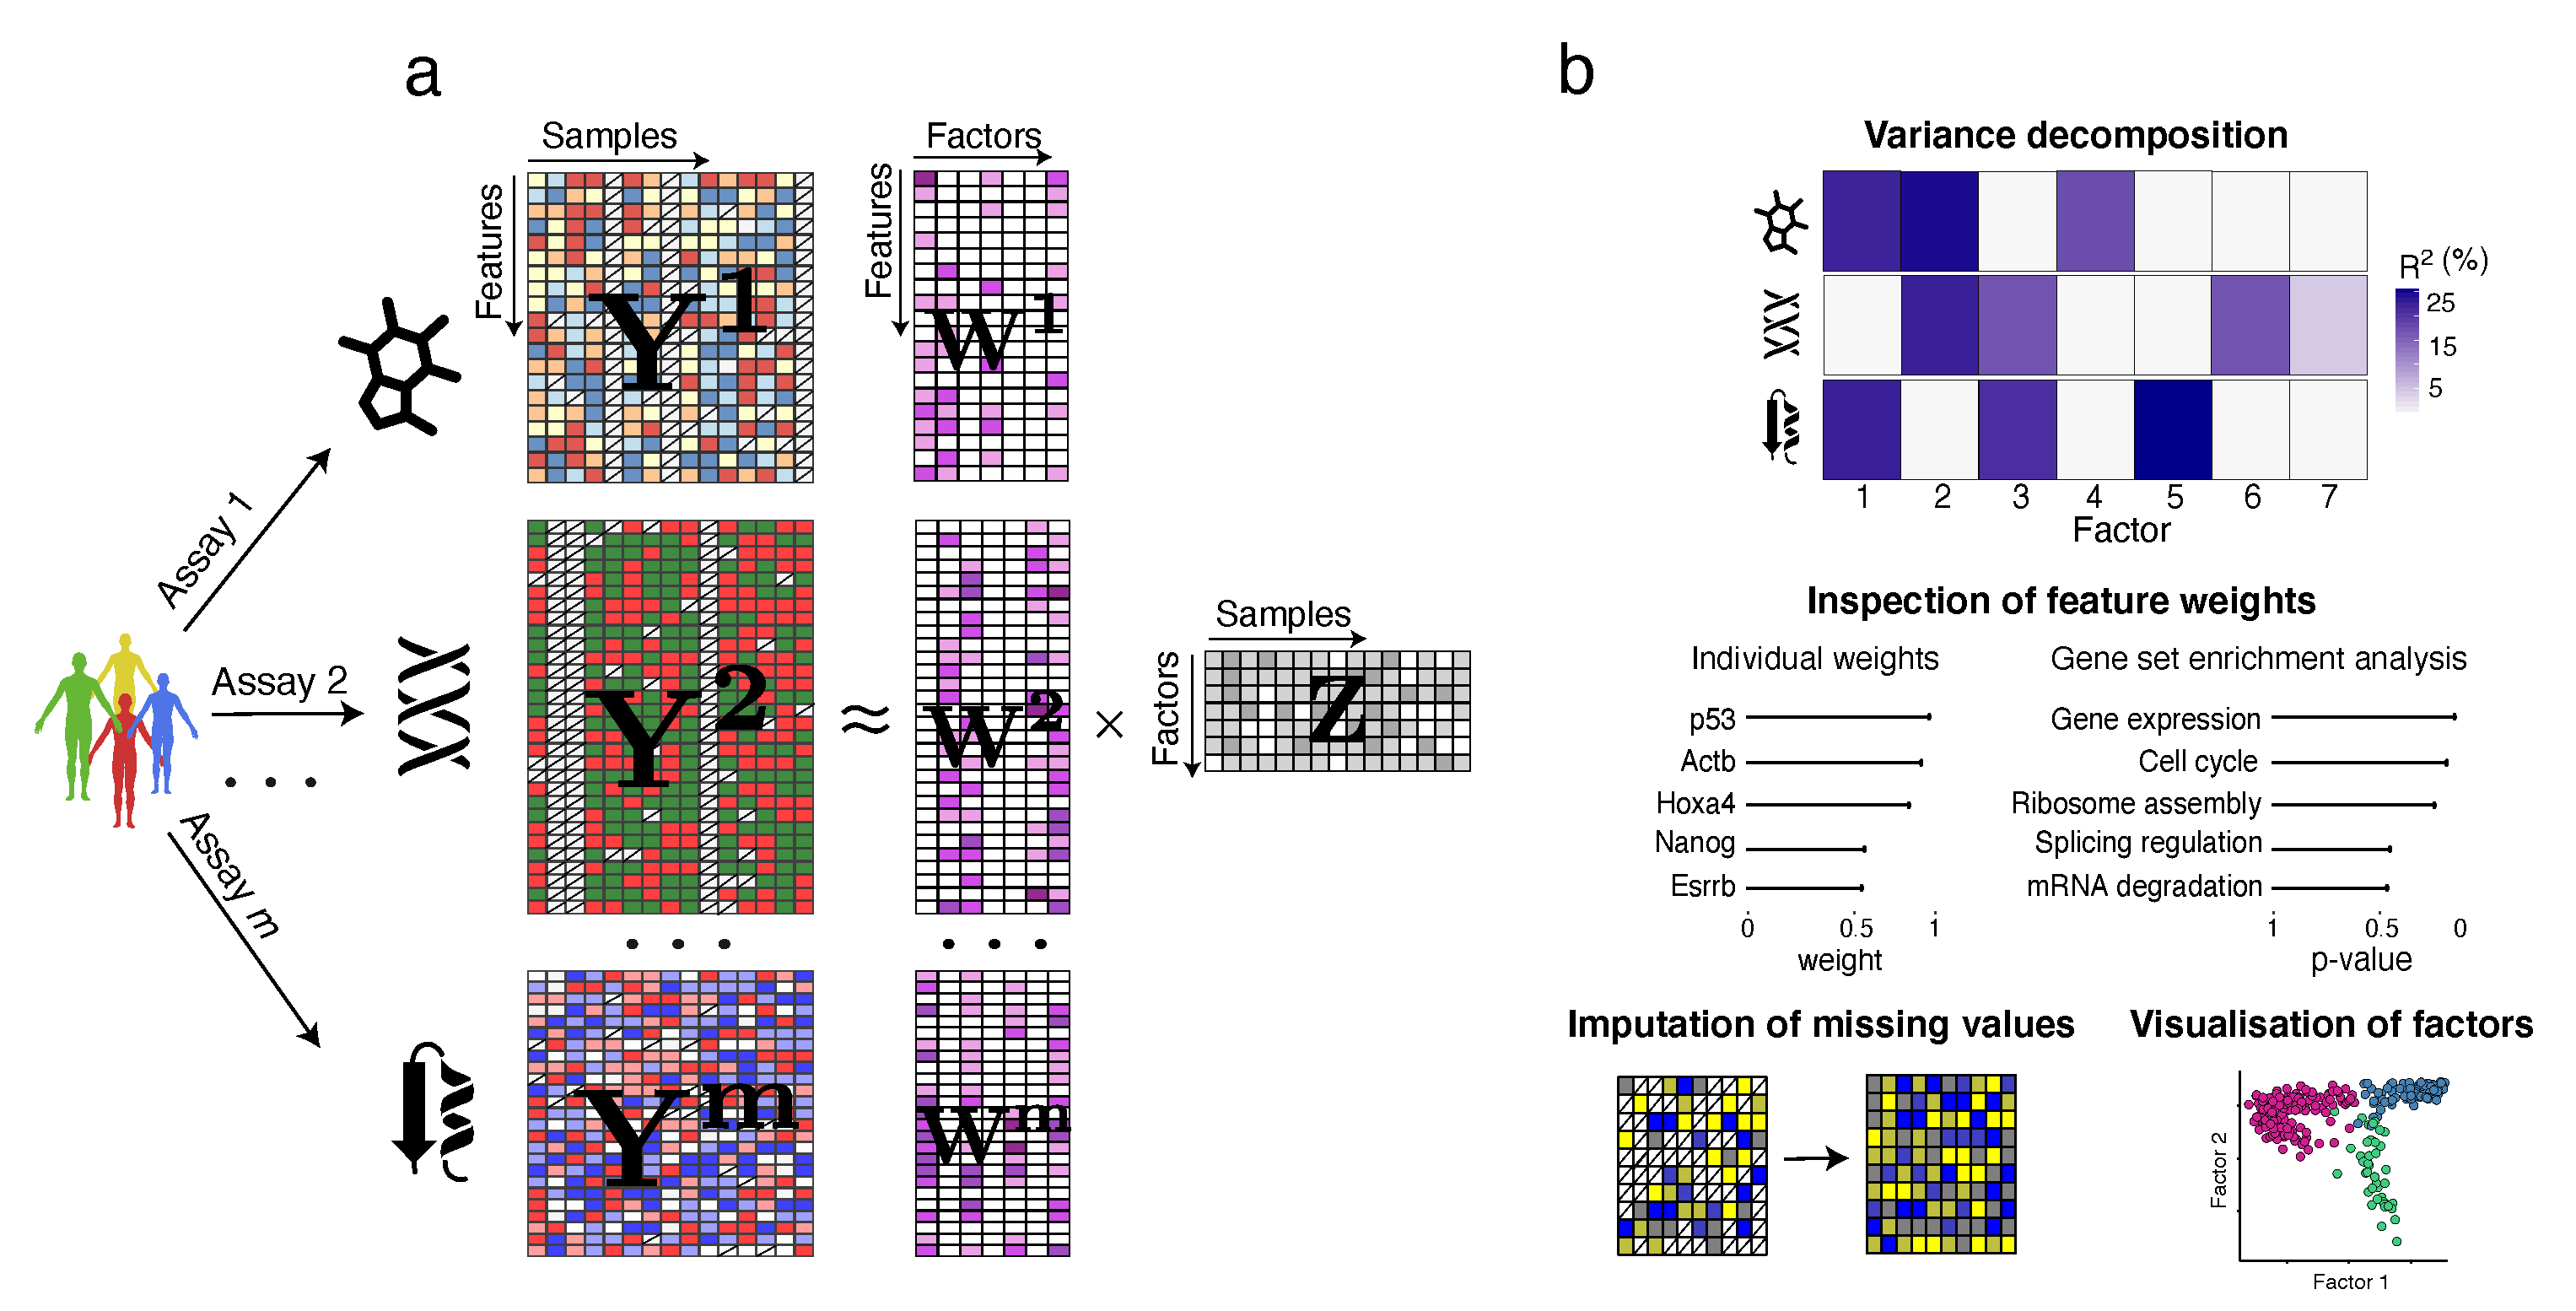
\includegraphics[width=1.0\textwidth]{MOFA}
		\caption{MOFA overview. The model takes $M$ data matrices as input ($\bfY^1, \cdots, \bfY^M$), one or more from each data modality, with co-occurrent samples but features that are not necessarily related and can differ in numbers. MOFA decomposes these matrices into a matrix of factors ($\bfZ$) and $M$ weight matrices, one for each data modality ($\bfW^1, \cdots, \bfW^M$). White cells in the weight matrices correspond to zeros, i.e. inactive features, whereas the cross symbol in the data matrices denotes missing values. The fitted MOFA model can be queried for different downstream analyses, including a variance decomposition to assess the proportion of variance explained by each factor in each data modality.}
		\label{fig:MOFA}
	\end{center}
\end{figure}

\begin{figure}[H]
	\centering
	% \definecolor{colD}{rgb}{0.2, 0.2, 0.6}
\definecolor{colM}{rgb}{0.0, 0.5, 0.0}
\definecolor{colN}{rgb}{0.5, 0.0, 0.13}
\definecolor{colG}{rgb}{1.0, 0.65, 0.0}
\newcommand\op{0.25}
\colorlet{shadecolor}{black!25}

\newcommand\op{0.25}

\begin{tikzpicture}
  % Define nodes:
  % matrix factorisation level
  \node[obs]   (Y) {$y_{n,d}^m$};
  \node[latent, above=of Y, xshift=-1.5cm] (Z) {$z_{n,k}$};
  \node[latent, above=of Y, xshift=1.5cm] (W) {$w_{k,d}^m$};
  \node[latent, xshift=1.5cm] (Tau) {$\tau_{d}^m$};

  % \node[opacity=\op,latent, xshift=-1.5cm] (Tau2) {$\tau_{n}$};

  % parents of Z
  \node[opacity=\op, det, above=of Z] (crossZ) {$\times$};
  \node[opacity=\op, latent, above=of crossZ] (Zhat) {$\hat{z}_{n,k}^{\ }$};
  \node[opacity=\op, latent, above=of Zhat] (SigmaZ) {$\alpha_k$};
  \node[opacity=\op, latent, above=of crossZ, xshift=-1.5cm] (SZ) {$s_{n,k}$};
  \node[opacity=\op, latent, above=of SZ] (ThetaZ) {$\theta_{k}$};

  % parents of W
  \node[det, above=of W] (crossW) {$\times$};
  \node[latent, above=of crossW] (What) {$\hat{w}_{k,d}^m$};
  \node[latent, above=of What] (SigmaW) {$\alpha_k^m$};
  \node[latent, above=of crossW, xshift=1.5cm] (SW) {$s_{k,d}^m$};
  \node[latent, above=of SW] (ThetaW) {$\theta_{k}^m$};

  % Connect the nodes
  \edge {Z,W, Tau} {Y}; %
  \edge[opacity=\op] {ThetaZ} {SZ};
  \edge[opacity=\op] {SigmaZ} {Zhat};
  \edge {ThetaW} {SW};
  \edge {SigmaW} {What};
  % \edge[opacity=\op] {Tau2} {Y}

  \factoredge[opacity=\op] {SZ, Zhat} {crossZ} {Z};
  \factoredge {SW, What} {crossW} {W};

  % cluster plate
  % \node[latent, above=of What, xshift=-1.3cm, opacity=0.15] (muW) {$\mu^m_{k, c}$};
  % \node[latent, above=of Zhat, xshift=1.3cm, opacity=0.15] (muZ) {$\mu_{k, c}$};
  % \edge[opacity=\op] {muZ} {Zhat};
  % \edge[opacity=\op] {muW} {What};
  % \plate[] {plateC} {(muZ)(muW)} {$C$};

  % Plates
  % \plate[] {plateK} {(Z)(W)(SZ)(Zhat)(SW)(What)(ThetaZ)(ThetaW)} {$K$};
  % \plate[color=colN, fill=colN, fill opacity=0.1] {plateN} {(Y)(Z)(crossZ)(Zhat)(SZ)(plateK.south west)} {\color{colN} $N$};
  % \plate[color=colD ,fill=colD, fill opacity=0.1] {plateD} {(Y)(W)(Tau)(crossW)(What)(SW)(plateK.south east) (plateN.south east)} {\color{colD}$D_m$};
  % \plate[color=colM,fill=colM, fill opacity=0.1] {plateM} {(plateD)(ThetaW)(plateK.north east)} {\color{colM}$M$};
  \plate[] {plateK} {(Z)(W)(SZ)(Zhat)(SW)(What)(ThetaZ)(ThetaW)} {$K$};
  \plate[] {plateN} {(Y)(Z)(crossZ)(Zhat)(SZ)(plateK.south west)} {$N$};
  \plate[] {plateD} {(Y)(W)(Tau)(crossW)(What)(SW)(plateK.south east) (plateN.south east)} {$D_m$};
  \plate[] {plateM} {(plateD)(ThetaW)(plateK.north east)} {$M$};

\end{tikzpicture}

	\caption{Graphical model for MOFA. The white circles represent hidden variables that are infered by the model, whereasa the grey circles represent the observed variables. There are a total of four plates, each one representing a dimension of the model: $M$ for the number of views, $N$ for the number of samples, $K$ for the number of factors and $D_m$ for the number of features in view $m$}
	\label{fig:MOFA_graphical_model}
\end{figure}

\subsubsection{Inference}
To make the model scalable to large data sets we adopt a Variational inference framework with a structured mean field approximation. 
A detailed overview is given in section XX, and details on the variational updates for the MOFA model are given in Appendix XX.\\
To enable efficient inference for non-Gaussian likelihoods we employ local bounds \cite{Jaakkola2000,Seeger2012}. This is described in detail in \Cref{section:mofa_ngaussian}

\subsection{Monitoring convergence}
An attractive property of Variational inference is that the objective function, the Evidence Lower Bound (ELBO), increases monotonically at every iteration. This provides a simple way of monitoring convergence \Cref{fig:elbo_convergence}. This is indeed one of the reasons why we opted for this inference framework over Expectation Propagation or sampling-based approaches.

 \begin{figure}[H]
	\centering 	
	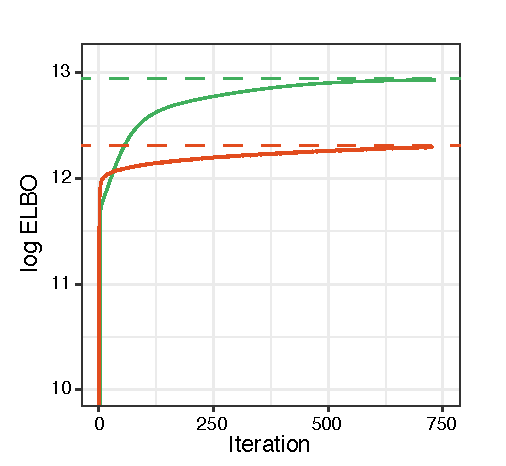
\includegraphics[width=0.5\textwidth]{elbo_convergence}
	\caption{Training curve for two diffent initialisations of MOFA. The y-axis displays the log of the ELBO, with higher values indicating a better fit. The x-axis displays the iteration number. The horizontal dash lines mark the value of the ELBO upon convergence. }
	\label{fig:elbo_convergence}
\end{figure}

\subsection{Model selection and consistency across random initilizations} \label{section:mofa_robustness}
The variational optimisation problem in MOFA is not convex and the posterior distributions will vary depending on the initialisation of the model. Thus, it becomes mandatory to perform model selection and assess the consistency of the factors across different trials.\\
The strategy we adopted in this work is to train several MOFA models (e.g. 10 trials) under different parameter initialisations, and after training we select the model with the highest ELBO for downstream analysis \Cref{fig:MOFA_robustness}. In addition, we evaluate the robustness of the factors by plotting the Pearson correlations between factors across all trials. \Cref{fig:MOFA_robustness}.\\
A similar strategy has also been proposed in \cite{Hore2016,Hore2015-thesis}.


\begin{figure}[H]
	\centering 	
	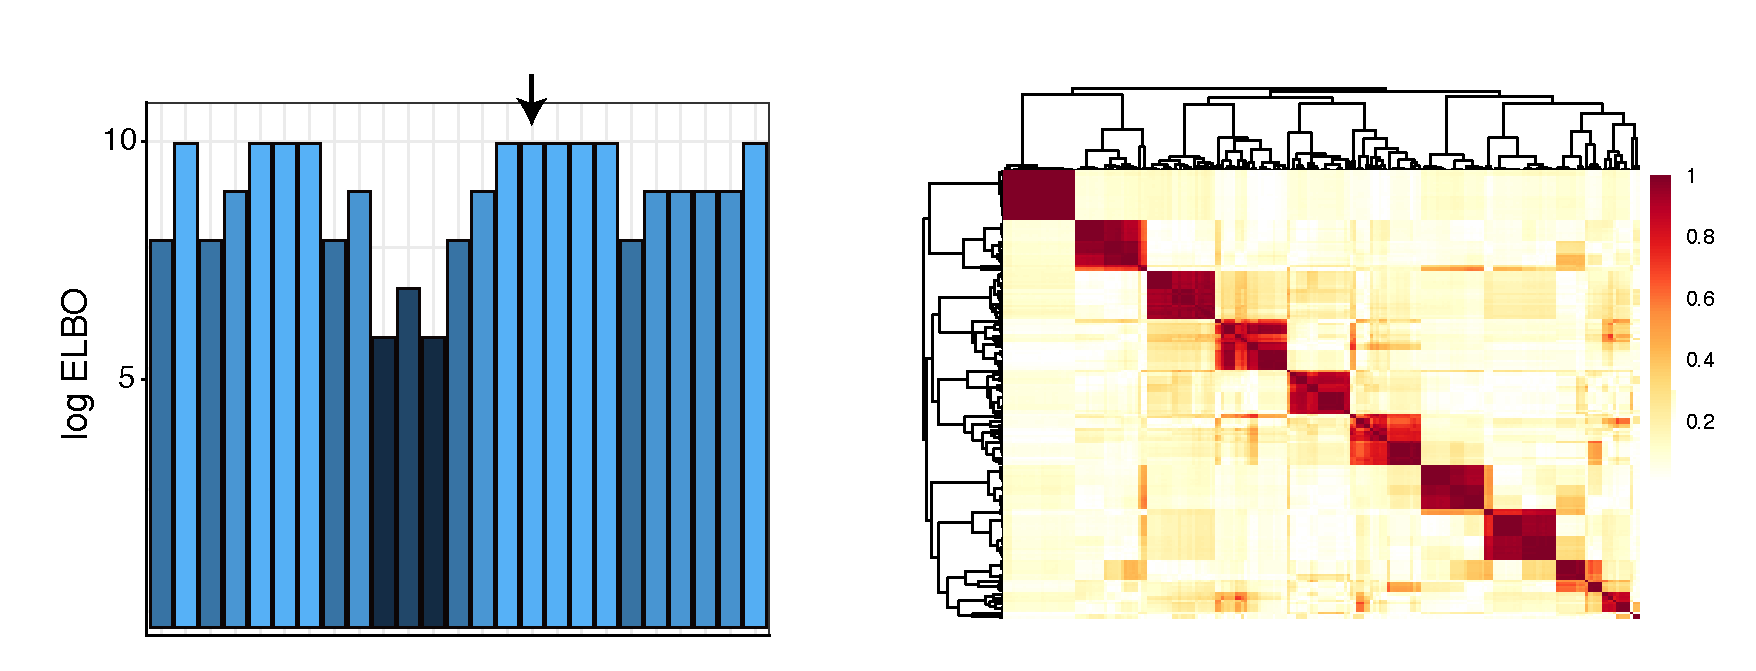
\includegraphics[width=1.0\textwidth]{MOFA_robustness}
	\caption{ Model selection and robustness analysis in MOFA. The left plot the log ELBO (y-axis) for 25 model instances (x-axis).
	The arrow indicates the model with the highest ELBO that would be selected for downstream analysis. The right plot displays the absolute value of the Pearson correlation coefficient between pairwise combinations of all factors across the 25 model instances. A block-diagonal matrix indicates that factors are robustly estimated regardless of the initialisation.}
	\label{fig:MOFA_robustness}
\end{figure}


% \subsection{Feature Set Enrichment Analysis}

% \subsection{Comparison with previous methods}

%The key difference with the sparse Bayesian factor analysis model in Section XX is that we learn a separate $\alpha_k^m$ and $\theta_k^m$ per factor and view, instead of per factor. This allows the model to take into account that the data is structured into different views.\\



\subsection{Learning the number of factors} \label{section:mofa_nfactors}
As described in section X, the use of an ARD prior allows factors to be actively prunned by the model if their variance explained is negligible. In the implementation we control the prunning of factors by a hyperparameter that defines a threshold on the minimum fraction of variance explained by a factor (across all views).\\
Additionally, because of the non-convexity of the optimisation problem, different model instances can potentially yield solutions with different number of active factors (\Cref{fig:mofa_nfactors}). Thus, the optimal number of factors can be selected by the model selection strategy outlined in \Cref{section:robustness}.

\begin{figure}[H]
	\centering 	
	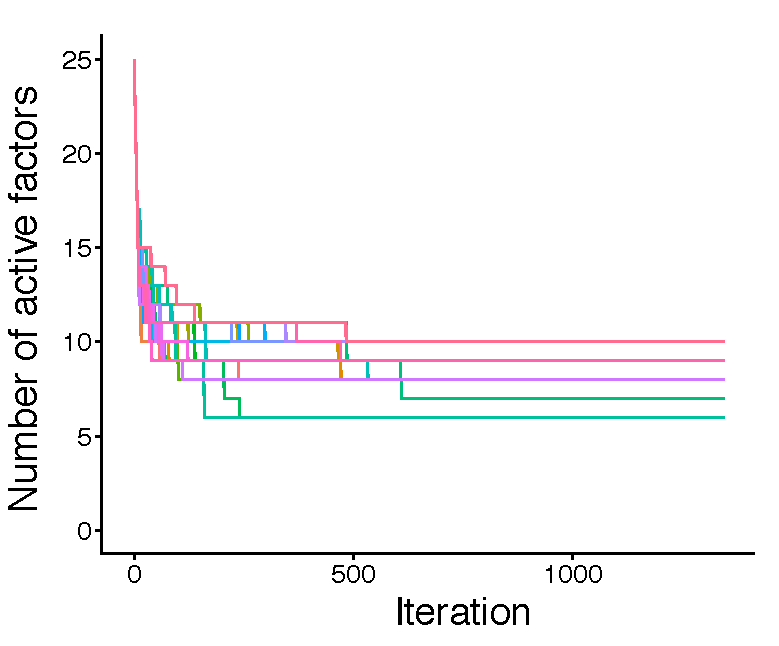
\includegraphics[width=0.5\textwidth]{MOFA_nfactors}
	\caption{Training curve for the number of active factors across 25 different model instances. The y-axis displays the number of active factors. The x-axis displays the iteration number. Different lines denote different model instances.}
	\label{fig:MOFA_nfactors}
\end{figure}


\subsection{Modelling and inference with non-Gaussian data} \label{section:mofa_ngaussian}
To implement efficient variational inference in conjunction with a non-Gaussian likelihood we adapt prior work from \cite{Seeger2012} using local variational bounds. The key idea is to dynamically approximate non-Gaussian data by Gaussian pseudo-data based on a second-order Taylor expansion.  To make the approximation justifiable we need to introduce variational parameters that are adjusted alongside the updates to improve the fit.	\\
Denoting the parameters in the MOFA model as $\bfX= (\bfZ,\bfW,\balpha,\btau,\btheta)$, recall that the variational framework approximates the posterior $p(\bfX | \bfY )$ with a distribution $q(\bfX)$, which is indirectly optimised by optimising a lower bound of the log model evidence. The resulting optimization problem can be re-written as
\begin{equation*}
\min_{q(\bfX)} -\Lagr(\bfX) =  \min_{q(\bfX)} \E_q \big[ -\log p(\bfY|\bfX) \big] + \KL[q(\bfX)||p(\bfX)].
\end{equation*}


Expanding the MOFA model to non-Gaussian likelihoods we now assume a general likelihood of the form $p(\bfY|\bfX)=p(\bfY|\bfC)$ with $\bfC = \bfZ\bfW^{T}$, that can write as

\begin{equation*}
-\log p(\bfY|\bfX) = \sum_{n=1}^{N} \sum_{d=1}^{D} f_{nd} (c_{nd})
\end{equation*}
with $f_{nd}(c_{nd}) = -\log p(y_{nd}|c_{nd})$. We dropped the view index $m$ to keep notation uncluttered.\\
Extending \cite{Seeger2012} to our heteroscedastic noise model, we require $f_{nd}(c_{nd})$ to be twice differentiable and bounded by $\kappa_d$, such that $f_{nd}''(c_{nd}) \leq \kappa_d \,\forall n,d$. This holds true in many important models as for example the Bernoulli and Poisson case. Under this assumption a lower bound on the log likelihood can be constructed using Taylor expansion,
\begin{equation*}
f_{nd}(c_{nd}) \leq \frac{\kappa_d}{2} (c_{nd} - \zeta_{nd})^2 + f'(\zeta_{nd})(c_{nd} - \zeta_{nd}) + f_{nd}(\zeta_{nd}) := q_{nd}(c_{nd},\zeta_{nd}),
\end{equation*}
where $\bZeta =  \zeta_{nd} $ are additional variational parameters that determine the location of the Taylor expansion and have to be optimised to make the lower bound as tight as possible. Plugging the bounds into above optimization problem, we obtain:
\begin{equation*}
\min_{q(\bfX),\bZeta} \quad \sum_{d=1}^{D}\sum_{n=1}^{N} \E_q [ q_{nd}(c_{nd},\zeta_{nd})] + \KL[q(\bfX)||p(\bfX)]
\end{equation*}
The algorithm propsed in \cite{Seeger2012} then alternates between updates of $\bZeta$ and $\mathrm{q}(\bTheta)$. The update for $\bZeta$ is given by
\begin{equation*}
\zeta \leftarrow \E[\bfW]\E[\bfZ]^{T}
\end{equation*}
where the expctations are taken with respect to the corresponding $q$ distributions.\\
% In order to find the updates for $q(\bTheta)$ we bring the taylor approximation of $q(f_{nd})$ in q audratic form:
% \begin{equation*}
% q(f_{nd},\zeta_{nd}) \propto \frac{\kappa_d}{2}(f_{nd} - (zeta_{nd} - g(\zeta_{nd})/\kappa_d))^2
% \end{equation*}
% and note that this is proportional to the log of a Gaussian distribution $-log \Normal (\hat{y}_{nd}|f_{ng},\frac{1}{ng})$ where $\hat{y}_{nd} = zeta_{nd} - g'(\zeta_{nd})/\kappa_d$ is defined as a pseudodata based on the zero-inflated observations.
% Consequently, for fixed $\zeta_{nd}$, the updates of the variational distributions $Q(X)$ and $Q(W)$ are equivalent to the ones derived in X, but with pseudodata $\hat{Y}$ and precision $\kappa_g$
On the other hand, the updates for $q(\bfX)$ can be shown to be identical to the variational Bayesian updates with a conjugate Gaussian likelihood when replacing the observed data $\bfY$ by a pseudo-data $\hat{\bfY}$ and the precisions $\tau_{nd}$ (which were treated as random variables) by the constant terms $\kappa_d$ introduced above.\\
The pseudodata is given by
\begin{equation*}
\hat{y}_{nd} = \zeta_{nd} - f'(\zeta_{nd})/\kappa_d.
\end{equation*}
Depending on the log likelihoods $f(\cdot)$ different $\kappa_d$ are used resulting in different pseudo-data updates. Two special cases implemented in MOFA are the Poisson and Bernoulli likelihood described in the following.

\subsubsection*{Bernoulli likelihood for binary data}
When the observations are binary, $y \in \{0,1\}$, they can be modelled using a Bernoulli likelihood:
%\begin{equation*}
%p(y|c) = \frac{e^{yc}}{1+e^c}
%\end{equation*}
%The second derivative of the log likelihood is bounded by:
%\begin{equation*}
%f''(c) = \sigma(c)\sigma(-c) \leq 1/4 := \kappa
%\end{equation*}
%where $\sigma$ is the sigmoid function $f(c) = 1/(1+e^{-c})$.\\
%The pseudodata updates are given by
%\begin{equation*}
%\hat{y}_{nd} = \zeta_{nd} - 4*(\sigma(\zeta_{nd}) - y_{nd})
%\end{equation*}
\begin{equation*}
\bfY|\bfZ,\bfW \sim \text{Ber}(\sigma(\bfZ\bfW^T)),
\end{equation*} where $\sigma(a)=(1+e^{-a})^{-1}$ is the logistic link function and $\bfZ$ and $\bfW$ are the latent factors and weights in our model, respectively.\\
In order to make the variational  inference efficient and explicit as in the Gaussian case, we aim to approximate the Bernoulli data by a Gaussian pseudo-data as proposed in \cite{Seeger2012} and described above which allows to recycle all the updates from the model with Gaussian views. While \cite{Seeger2012} assumes a homoscedastic approximation with a spherical Gaussian, we adopt an approach following \cite{Jaakkola2000}, which allows for heteroscedaticity and provides a tighter bound on the Bernoulli likelihood.\\
Denoting $c_{nd}=(\bfZ\bfW^T)_{nd}$ the Jaakkola upper bound \cite{Jaakkola2000} on the negative log-likelihood is given by
\begin{align*}
\begin{split}
-\log\left(p(y_{nd}|c_{nd})\right) &= -\log\left(\sigma\left((2y_{nd}-1)  c_{nd}\right)\right)\\
& \leq -\log(\zeta_{nd})-\frac{(2y_{nd}-1)c_{nd}-\zeta_{nd})}{2} +\lambda(\zeta_{nd})\left(c_{nd}^2 -\zeta_{nd}^2 \right)\\
& =: b_J(\zeta_{nd}, c_{nd},y_{nd} )
\label{jaakkola}
\end{split}
\end{align*}
with $\lambda$ given by $\lambda(\zeta)=\frac{1}{4\zeta}\tanh\left(\frac{\zeta}{2}\right)$.\\
This can easily be derived from a first-order Taylor expansion on the function $f(x) = - \log(e^{\frac{x}{2}}+e^{-\frac{x}{2}}) = \frac{x}{2}-\log(\sigma(x))$ in $x^2$ and by the convexity of 
$f$ in $x^2$ this bound is global as discussed in \cite{Jaakkola2000}.\\
In order to make use of this tighter bound but still be able to re-use the variational updates from the Gaussian case we re-formulate the bound as a Gaussian likelihood on pseudo-data $\hat{\bfY}$.\\
As above we can plug this bound on the negative log-likelihood into the variational optimization problem to obtain  \begin{equation*}
\min_{q(\bfX),\bZeta} \quad \sum_{d=1}^{D}\sum_{n=1}^{N} \mathbb{E}_q b_J(\zeta_{nd}, c_{nd},y_{nd} ) + \KL[q(\bfX)||p(\bfX)].
\end{equation*}
This is minimized iteratively in the variational parameter $\zeta_{nd}$ and the variational distribution of Z,W:\\
Minimizing in the variational parameter $\zeta$ this leads to the updates given by
\begin{equation*}
\zeta_{nd}^2 = \mathbb{E}[c_{nd}^2]
\end{equation*}
as described in \cite{Jaakkola2000}, \cite{Bishop}.\\
For the variational distribution $q(\bfZ,\bfW)$ we observe that the Jaakkola bound can be re-written as 
\begin{equation*}
b_J(\zeta_{nd}, c_{nd},y_{nd} ) = -\log\left(\varphi\left(\hat{y}_{nd}; c_{nd}, \frac{1}{2\lambda(\zeta_{nd})}\right)\right) + \gamma(\zeta_{nd}),
\end{equation*}
where $\varphi(\cdot; \mu, \sigma^2)$ denotes the density function of a normal distribution with mean $\mu$ and variance $\sigma^2$ and $\gamma$ is a term only depending on $\bZeta$. This allows us to re-use the updates for $\bfZ$ and $\bfW$ from a setting with Gaussian likelihood by considering the Gaussian pseudo-data 
\begin{equation*}
\hat{y}_{nd}= \frac{2y_{nd}-1}{4 \lambda(\zeta_{nd})}
\end{equation*}
updating the data precision as $\tau_{nd} = 2\lambda(\zeta_{nd})$ using  updates generalized for sample- and feature-wise precision parameters on the data.


\subsubsection*{Poisson likelihood for count data}
When observations are a natural numbers, such as count data $y \in \N = \{0,1,\cdots\}$, they can be modelled using a Poisson likelihood:
\begin{equation*}
p(y|c) = \lambda(c)^y e^{-\lambda(c)}
\end{equation*}
where $\lambda(c)>0$ is the rate function and has to be convex and log-concave in order to ensure that the likelihood is log-concave.\\
As done in \cite{Seeger2012}, here we choose the following rate function: $\lambda(c)=\log(1+e^c)$.

Then an upper bound of the second derivative of the log-likelihood is given by
\begin{equation*}
f''_{nd}(c_{nd}) \leq \kappa_d = 1/4 + 0.17*\max(\bfy_{:,d}).
\end{equation*}
%The bound degrades with the presence of entries with large values. Thus, we follow common practice and clip overly large counts.\\
The pseudodata updates are given by
\begin{equation*}
\hat{y}_{nd} = \zeta_{nd} - \frac{\mathrm{S}(\zeta_{nd})(1-y_{nd}/\lambda(\zeta_{nd}))}{\kappa_d}.
\end{equation*}


\subsection{Model validation with simulated data} \label{section:mofa_simulated}
We used simulated data from the generative model to systematically test the technical capabilities of MOFA.





\subsubsection{Recovery of the latent space}
First, we tested the ability of MOFA to recover simulated factors, varying the number of views, the number of features, the number of factors and the fraction of missing values.\\ 
For every simulation scenario we initialised a model with a high number of factors ($K=100$), and inactive factors were automatically dropped during model training using a threshold of 1\% variance explained. In addition, to test the robustness under different initialisations, ten models were trained for every simulation scenario.\\
We observe that in most settings the model accurately recovers the correct number of factors (\Cref{fig:MOFA_learnK}). Exceptions occur when the dimensionality of the latent space is too large (more than 50 factors) or when an excessive amount of missing values (more than 80\%) is present in the data.

\begin{figure}[H]
	\centering 	
	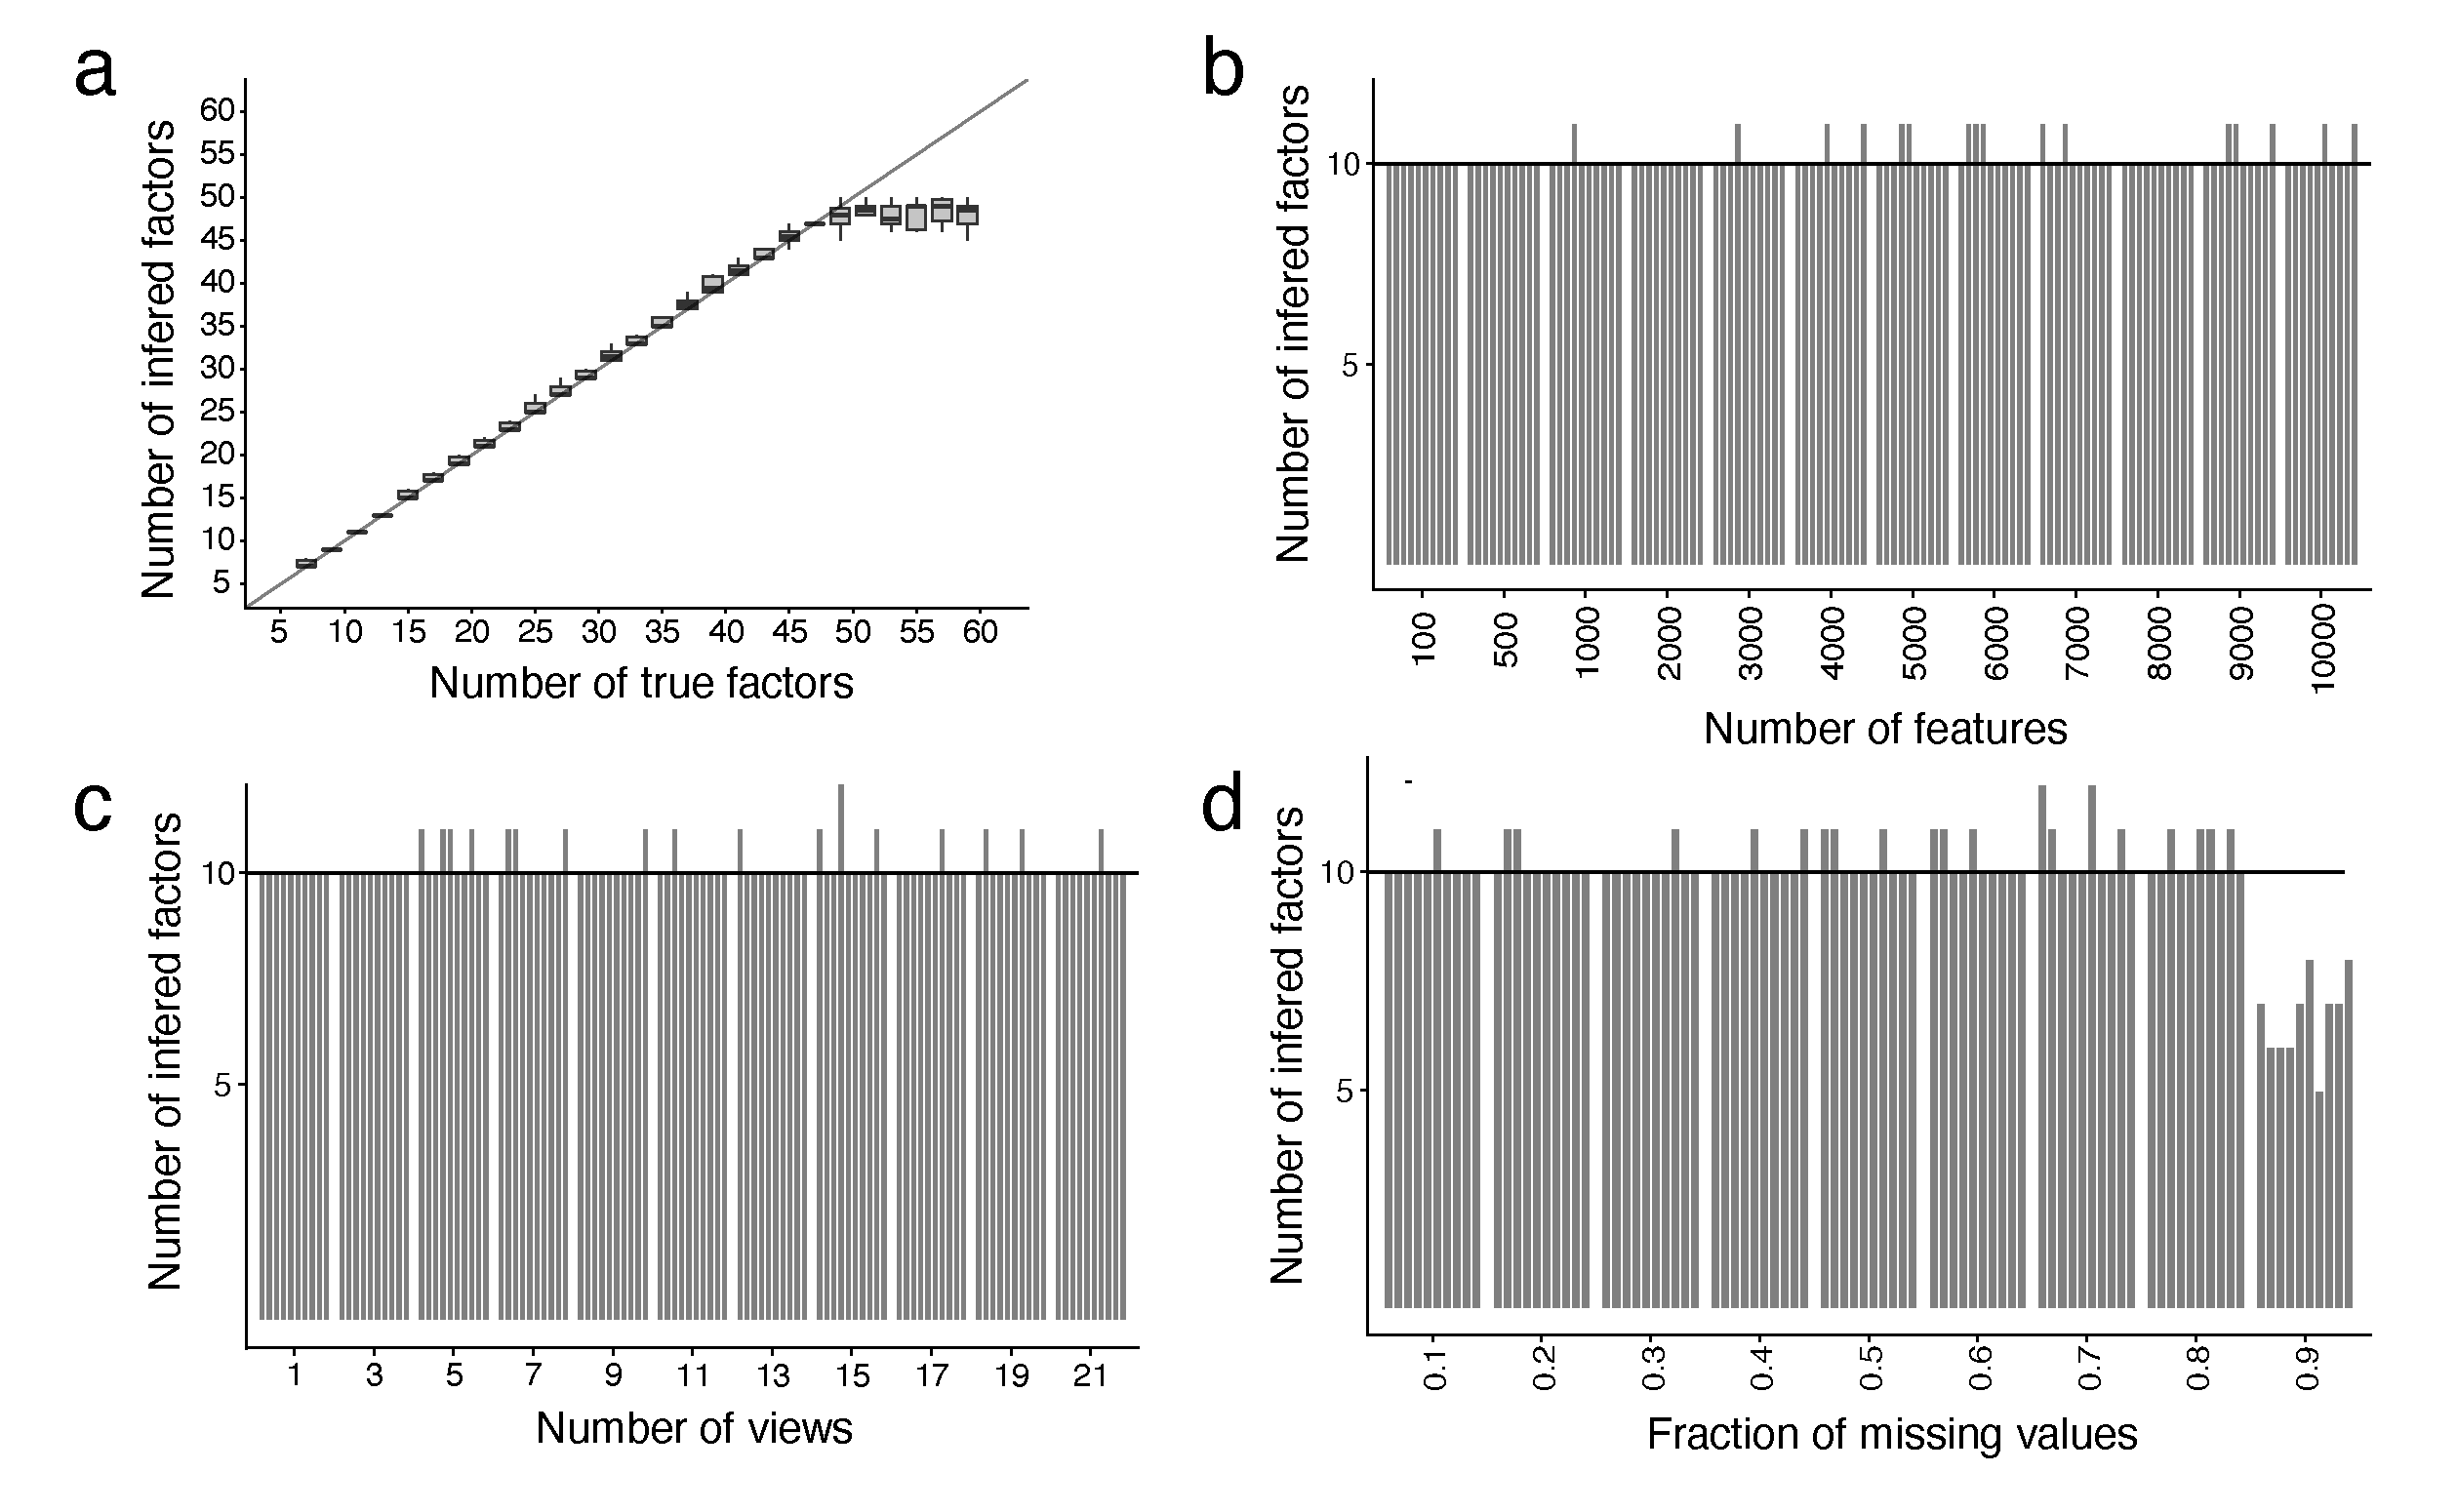
\includegraphics[width=1.0\textwidth]{MOFA_learnK}
	\caption{Assessing the ability of MOFA to recover simulated latent spaces. In all plots the y-axis displays the number of infered factors. (a) x-axis displays the number of true factors, and boxplots summarise the distribution across 10 model instances. For (c-d) the true number of factors was set to $K=10$ and each bar corresponds to a different model instance. (b) x-axis displays the number of features, (c) x-axis displays the number of views, (d) x-axis displays fraction of missing values. }
	\label{fig:MOFA_learnK}
\end{figure}

\subsubsection{Group-wise sparsity on the loadings}
One of the most important statistical assumptions underlying MOFA (and other Group Factor Analysis methods) is the sparsity prior aimed at disentangling the activity of factors across views.\\
To evaluate this feature we simulated data from the generative model were the factors were clearly set to be active or inactive in specific views. We compared the performance with two other methods: the iCluster+ model \cite{Mo2013} and a GFA implementation \cite{Leppaaho2017}.\\
the GFA implementation shares the same factor and view-wise sparsity as MOFA, and is therefore expected to show similar performance. On the other hand, iCluster is a model that is aimed at clustering and it only contains a sparsity constraint (in a penalised maximum likelihood setting) per factor, shared across all views.\\
On simulated data, MOFA and GFA correctly infer the true activity pattern of the factors whereas iCluster infers incorrect sharedness of factors across views, especially with increasing dimensionality of the latent space.

\begin{figure}[H]
	\centering 	
	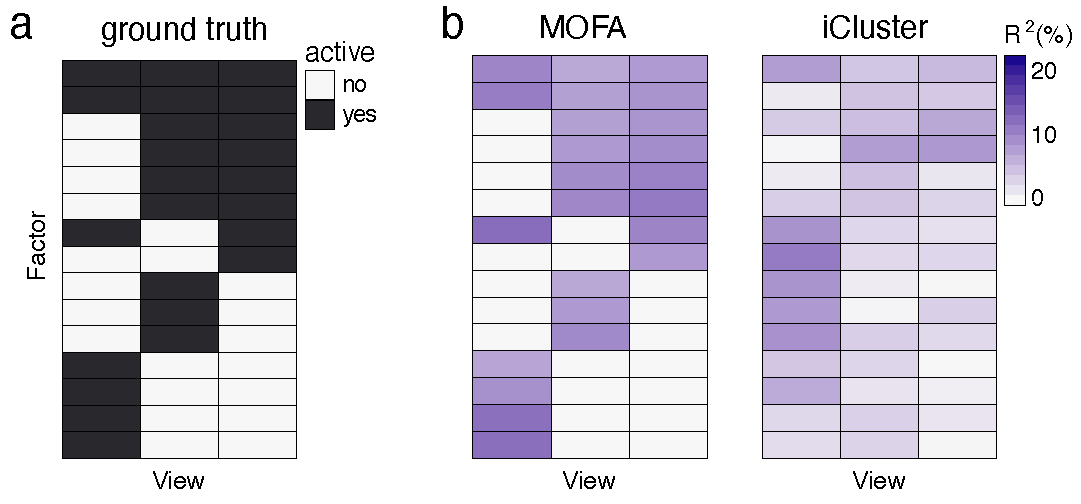
\includegraphics[width=1.0\textwidth]{MOFA_group_sparsity}
	\caption{Evaluating the ability of MOFA, iCluster and GFA to recover sparse factor activity patterns across views. The leftmost plot displays the true activity pattern, with factors being (strongly) active in different subsets of views. The remaining three plots show, for each model, the fraction of variance explained ($R^2$) by each factor in each view.}
	\label{fig:MOFA_group_sparsity}
\end{figure}

\subsubsection{Feature-wise sparsity on the loadings}
A key aspect of MOFA is the use of a spike-and-slab prior distribution to enforce feature-wise sparsity on the loadings, which yields a more interpretable solution (see \Cref{section:mofa_priors}).\\
To assess the effect of the spike-and-slab prior we fit a group of models with a spike-and-slab prior and another group of models only with Automatic Relevance Determination prior. We further compared both solutions to a conventional Principal Component Analysis fit on the concatenated data set.\\
As expected, we observe that the spike-and-slab prior induces more zero-inflated weights, although the ARD prior provided a moderate degree of regularisation. The PCA solution was notably more dense than both bayesian models (\Cref{fig:MOFA_sparsity}).

\begin{figure}[H]
	\centering 	
	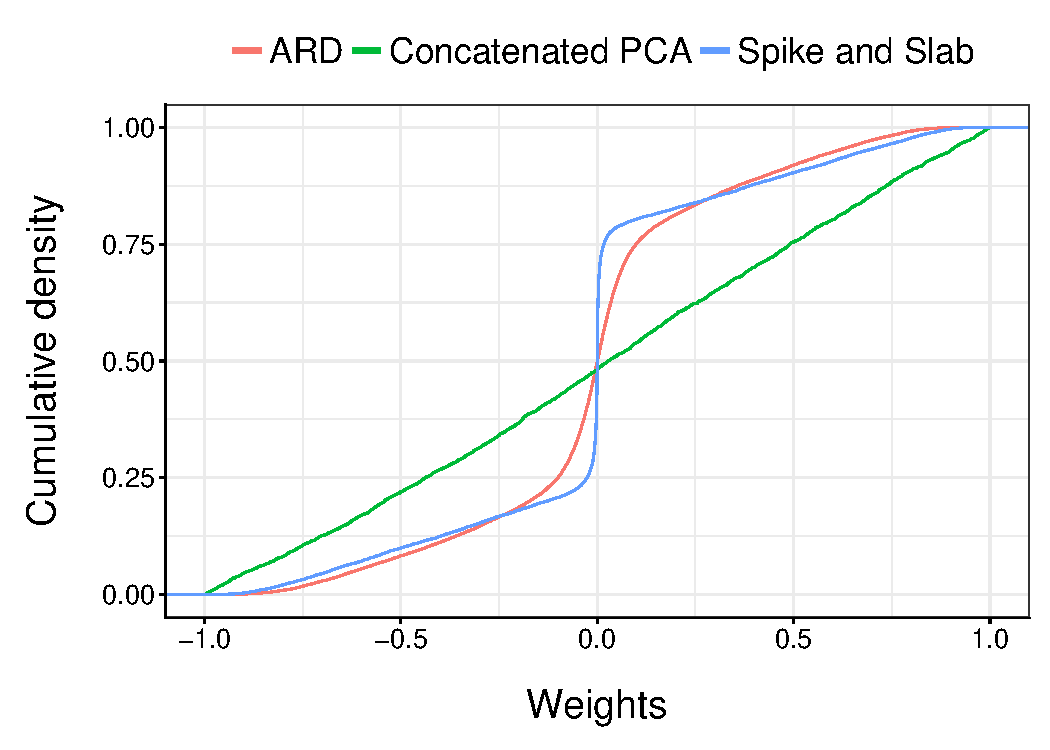
\includegraphics[width=0.7\textwidth]{MOFA_sparsity}
	\caption{Assessing sparsity on the loadings in MOFA. The plot shows the empirical cumulative density function of the loadings for an arbitrary factor in a single view. The loadings were simulated with a sparsity level of $\theta_k^m=0.5$ (50\% of active features.)
	}
	\label{fig:MOFA_sparsity}
\end{figure}


\subsubsection{Non-gaussian likelihoods}
A key improvement of MOFA with respect to previous methods is the use of non-Gaussian likelihoods to integrate multiple data modalities. As described in section XX, we implemented a Bernoulli likelihood to model binary data and a Poisson likelihood to model count data.\\
To validate both likelihood models, we simulated binary and count data using the generative model and we fit two sets of models for each data type: a group of models with a Gaussian likelihood and a group of models with a Bernoulli or Poisson likelihood, respectively.\\
We observe that although both likelihoods are able to recover the true number of factors, the models with the non-Gaussian likelihoods clearly result in a better fit to the data (\Cref{fig:MOFA_nongaussian_binary,fig:MOFA_nongaussian_poisson}).

\begin{figure}[H]
	\centering 	
	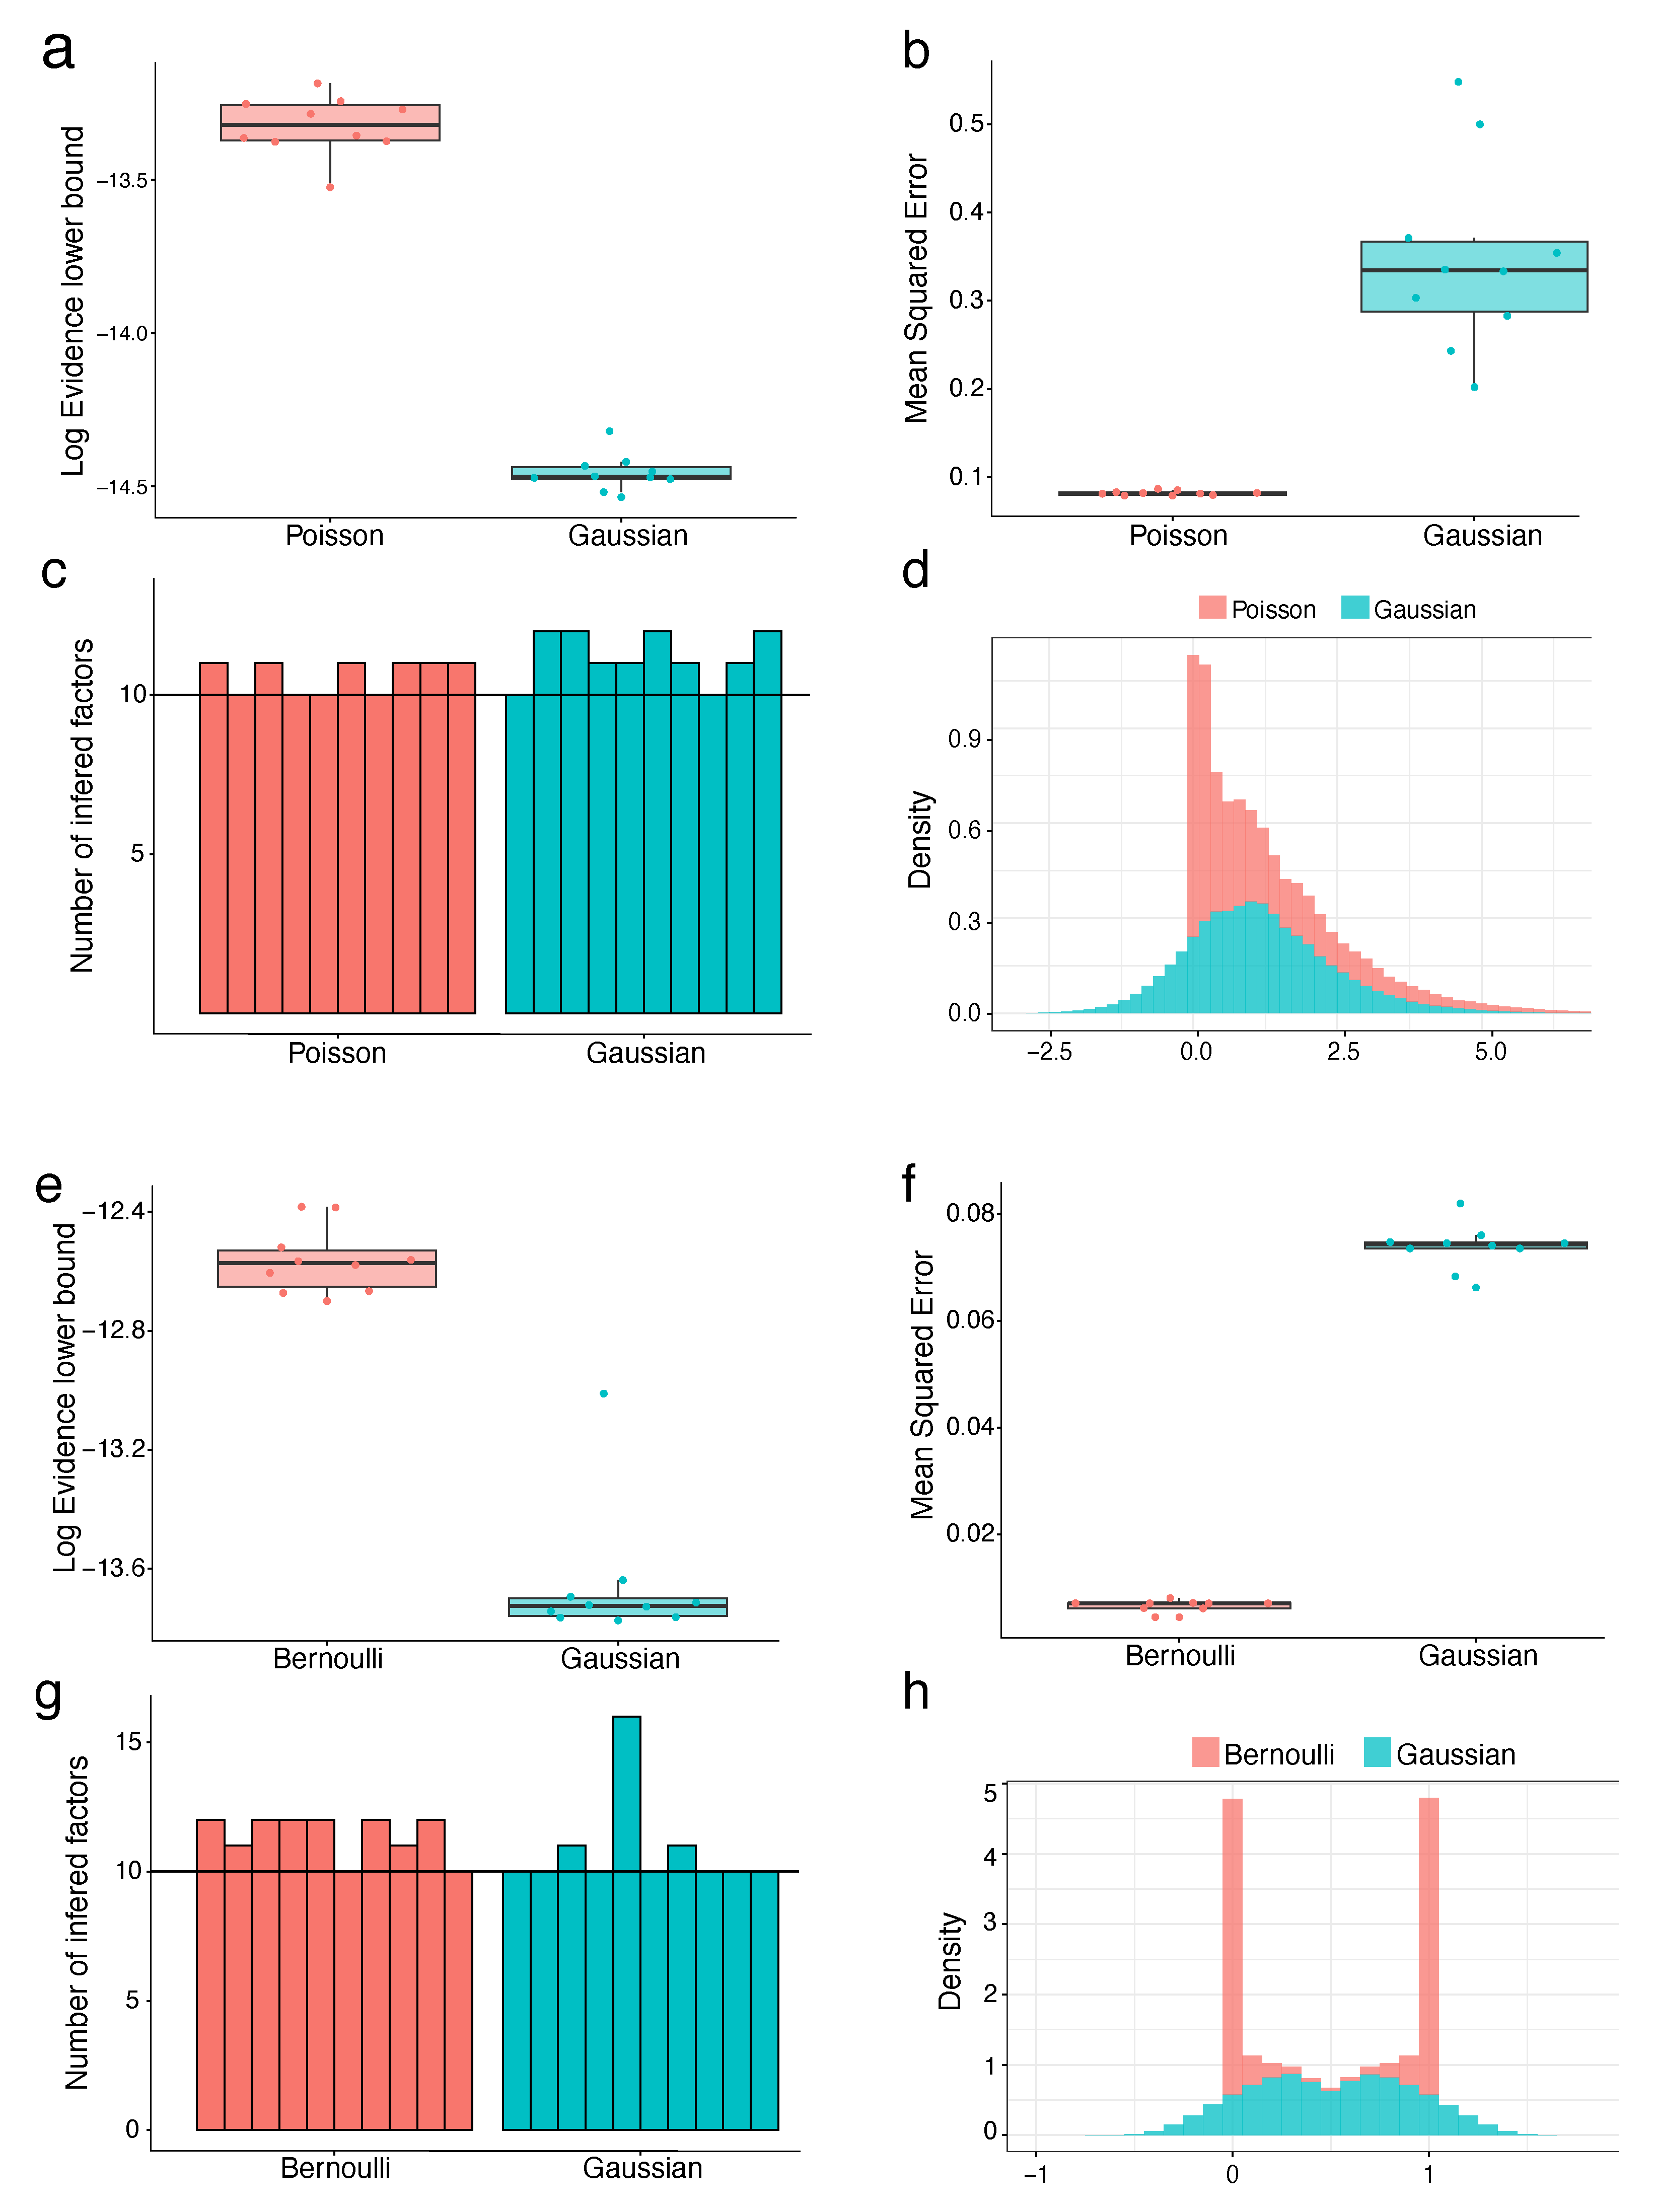
\includegraphics[width=1.0\textwidth]{MOFA_nongaussian}
	\caption{Validation of the non-gaussian likelihood models implemented in MOFA on simulated data. The four plots on the left assess the Poisson and the Gaussian likelihoods applied to count data. The four plots on the right assess the Bernoulli and the Gaussian likelihoods applied to binary data. (a) The y-axis displays the ELBO for each model instance (x-axis). (b) The y-axis displays the mean reconstruction error for each model instance (x-axis). (c) The y-axis displays the number of estimated factrors for each model instance (x-axis). The horizontal dashed line marks the true number of factors $K=10$. (d) Distribution of reconstructed data.}
	\label{fig:MOFA_nongaussian}
\end{figure}


\subsubsection{Scalability}
Finally, we evaluated the scalability of the model when varying each of its dimensions independently (\Cref{fig:MOFA_scalability}), and we compared the speed with a Gibbs sampling implementation of GFA \cite{Leppaaho2017} and iCluster+ \cite{Mo2013}.\\
Overall, we observe that MOFA scales linear with respect to all dimensions and is significantly faster than any of the three evaluated techniques.\\
As a real application showcase, the training on the CLL data \Cref{fig:MOFA_CLL_Figure1} required 25 minutes using MOFA, 34 hours with GFA and 5-6 days with iCluster.

\begin{figure}[H]
	\centering 	
	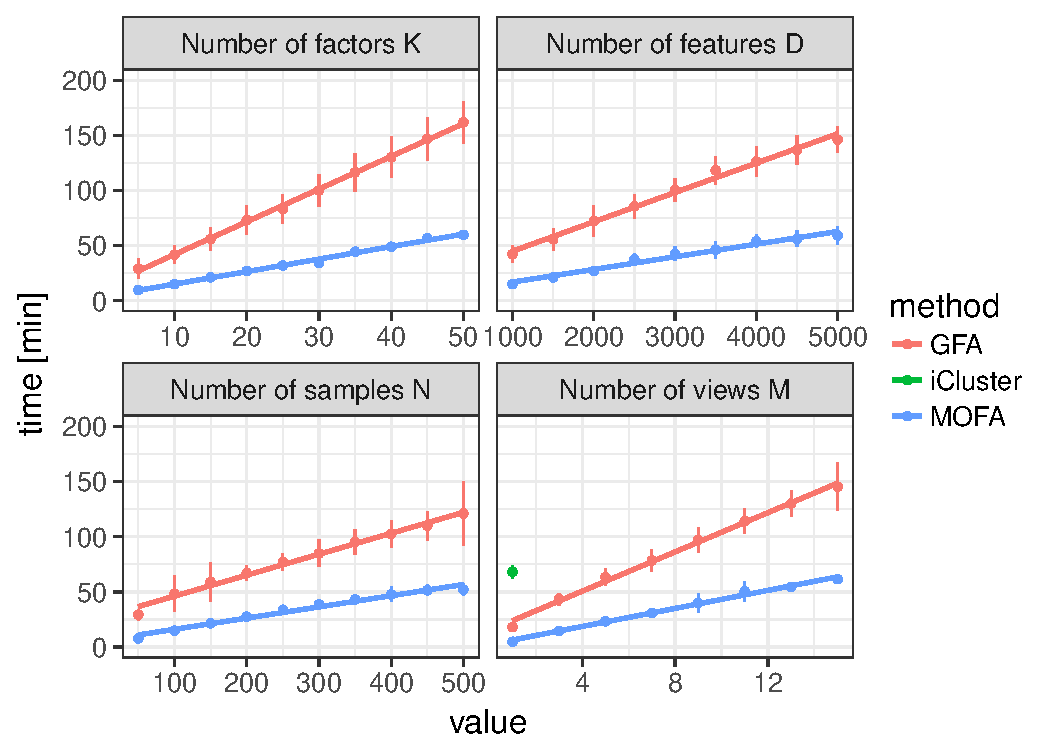
\includegraphics[width=0.9\textwidth]{MOFA_scalability}
	\caption{Evaluation of speed and scalability in MOFA. The y-axis displays the time required for convergence. The x-axis displays the value of the dimension that was tested, either number of factors ($K$), number of features ($D$), number of samples ($N$) and number of views ($M$). Baseline parameters were $M=3, K=10, D=1000, N=100$. Each line represents a different model, GFA (red), MOFA (blue) and iCluster (green). Default convergence criteria where used for all methods. Each dot displays the average time across 10 trials with error bars denoting the standard deviation. iCluster is only shown for one value as all other settings required more than 200min for convergence.
	}
	\label{fig:MOFA_nongaussian}
\end{figure}



\subsection{Application to chronic lymphocytic leukaemia} \label{section:mofa_cll}
Personalised medicine is an attractive field for the use of multi-omics, as dissecting heterogeneity across patients is a major challenge in complex diseases, and requires integration of information from multiple biological layers \cite{Chen2013,Costello2014,Alyass2015}.\\
In most cases, predicting patient survival and response to a treatment is still not reliable due to a lack of predictive biomarkers and our incomplete understanding of the mechanisms underlying response heterogeneity. Identification of the main drivers of inter-patient variation and their molecular basis is an important step towards personalized treatment decisions. 

To demonstrate the potential of the method, we applied MOFA to a study of 200 patient samples of chronic lymphocytic leukaemia (CLL) profiled for somatic mutations, RNA expression, DNA methylation and ex-vivo drug responses\cite{Dietrich2018} \Cref{fig:MOFA_CLL_Figure1}.\\

This data set was selected for five main reasons. 
\begin{itemize}
	\item The large number of cases to benchmark the speed of MOFA against other common integrative methods.
	\item The rich literature in this type of cancer which provides a good resource for the interpretation of the factors.
	\item The complex missing data structure of the study, with nearly 40\% samples having incomplete assays \Cref{fig:MOFA_CLL_Figure1}, in addition to the missing values present within some assays. hence, this study is ideal to benchmark MOFA's capabilities to deal with missing entries. As described in Section X, the inference framework we implemented allows the model to cope with this setting by merely ignoring missing entries and, when possible, pooling information from other molecular layers in order to infer the factor values.
	\item The different data modalities: after data processing, three assays had continuous observations whereas for the somatic mutations the observations were binary. As described in section XX, MOFA can combine different likelihood models to integrate multiple data types.
	\item The existence of clinical covariates: after model fitting, the factors can be associated with additional covariates. This provides an excellent test to assess whether the MOFA factors can capture the clinical phenotypes better than other dimensionality reduction techniques.
\end{itemize}


\subsubsection{Model overview}
In this data set, MOFA recovered 10 factors explaining a minimum of 3\% of variance. Among these, the first two factors (sorted by variance explained) were active across most views, indicating a strong effect across multiple molecular layers. Other factors such as Factor 3 or Factor 5 explained variation in two data modalities, whereas Factor 4 was only in the RNA expression data.\\
Overall, the then MOFA factors inferred explained 41\% of variance in the drug response data, 38\% in the mRNA expression, 24\% in the DNA methylation and 24\% in somatic mutations.

Inspection of the top weights in the somatic mutation view revealed that Factor 1 was strongly associated with the mutation status of the immunoglobulin heavy-chain variable (IGHV) region, while Factor 2 was aligned with a trisomy of chromosome 12 (Figure X). In a completely unsupervised fashion, MOFA identified the two major axes of molecular disease heterogeneity being indeed the two most important clinical markers in CLL \cite{Fabbri2016,Zenz2010}.\\
A scatterplot based on these factors shows a clear separation of patients by their IGHV status on the first factor and presence or absence of trisomy 12 on the second factor. Remarkably, the IGHV status of a fraction of patients was missing (grey dots). Yet, as the two factors were shared across multiple views, MOFA was able to pool information from the other molecular layers to map those samples to the latent space.

\begin{figure}[H]
	\centering 	
	\includegraphics[width=1.0\textwidth]{MOFA_CLL_Figure1}
	\caption{XX}
	\label{fig:MOFA_CLL_Figure1}
\end{figure}

\subsubsection{Characterisation of Factor 1}

IGHV status is probably the most important prognostic marker in CLL and has routinely been used to distinguish between two distinct subtypes of the disease. Molecularly, it is a surrogate of the level of activation of the B-cell receptor, which is in turn related to the differentiation state of the tumoral cells. Multiple studies have associated mutated IGHV with a better resposne to chemoimmunotherapy, whereas unmutated IGHV patients have a worse prognosis \cite{Fabbri2016,Bulian2017,Crombie2017,Damle1999}.\\

In clinical practice, the IGHV status has been generally considered binary. However, our results suggest a more complex structure with at least three groups or a potential underlying continuum, as also suggested in \cite{Oakes2016,Queiros2015}.\\
Interestingly, there is some discrepancy between the IGHV status predicted by MOFA and the IGHV status reported in the clinical data. Out the 200 patients, MOFA classifies 176 in accordance with the clinical label, it classifies 12 patients that lacked the clinical marker and it re-classifies 12 patients to the opposite group.\\
To validate the MOFA-based classification, we inspected the molecular profiles. sample-to-sample correlation matrices for the individual layers suggest that for 3 of the cases where the inferred factor disagrees with the clinical label, the molecular data supports the predicted label. The other 9 cases showed intermediate molecular sgnatures now well captured by the binary classification.\\
%Based on these results, we hypothesize that a multi-omics approach based on several molecular signatures could be a more precise and robust approach to predict clinical phenotypes than the use of single features such as mutations or expression of marker genes.

\begin{figure}[H]
	\centering 	
	\includegraphics[width=1.0\textwidth]{MOFA_IGHV_outlier}
	\caption{XX}
	\label{fig:MOFA_IGHV_outlier}
\end{figure}


Finally, we characterised in more detail the molecular changes associated with IGHV status, as predicted by MOFA.\\
On the RNA expression, inspection of the top weights pinpoint genes that have been previously associated to IGHV status, some of which have been proposed as clinical markers\cite{Vasconcelos2005,Maloum2009,Trojani2011,Morabito2015,Plesingerova2017}. Heatmaps of the RNA expression levels for these genes reveals clear differences between samples when ordered according to the corresponding Factor 1 values.\\
On the drug response data the loadings highlight kinase inhibitors targeting the B-cell receptor pathway. Splitting the patients into three groups based on k-means clustering shows clear separation in the drug response curves.

\begin{figure}[H]
	\centering 	
	\includegraphics[width=1.0\textwidth]{MOFA_CLL_Factor1}
	\caption{XX}
	\label{fig:MOFA_CLL_Factor1}
\end{figure}

\subsubsection{Characterisation of other Factors}
% While the well-known clinical markers such as IGHV status and the more recently studied trisomy 12 are identified as most important sources of variation, they explain less than 20% variability in any view, suggesting the existence of more subtle sources of variation. 
% As an example, we further investigated latent factor 5, which explains 2% variation in the mRNA view and 6% of variation in the drug response view and is highly enriched for oxidative stress and senescence pathways in the mRNA view (Figure S12a). In particular, the top weights correspond to heat shock proteins (HSPs) such as HSPA1A, HSPA1B and HSPA6 (Figure S12b), a group of proteins that are essential for protein stability which are up-regulated upon stress conditions like high temperatures, pH shift or oxidative stress. Importantly, in tumour cells, including CLL, HSPs have been described to be elevated and may contribute to prolonged tumour cell survival (Dempsey et al. 2010a).
% In agreement with the findings from the mRNA view, the drugs with largest weights on factor 5 belong to clinical categories also associated with stress response, such as target reactive oxygen species (SD07, MIS-43, SD51) and DNA damage response (fludarabine, nutlin-3, doxorubicine) (Figure S12c-d). In particular, patients with high expression of HSPs display higher viability to the aforementioned drugs.

\subsubsection{Prediction of clinical outcomes}


We conjectured that the integration of the multiple molecular layers could allow a better prediction of clinical response compared to using single omics or naïve data integration.\\
To evaluate the utility of the MOFA factors as predictors of clinical outcomes we fit Cox regression models \cite{Cox1972} using the patients’ time to next treatment (TTT) as a response variable. Two types of analysis were performed: a univariate analysis where each Factor was independently associated with TTT, and a multivariate analysis where the combination of all Factors were used to predict TTT.\\

(CHECK) In the univariate Cox models, we observe  that Factor 1 (IGHV status), Factor 7 (associated with chemo-immunotherapy treatment prior to sample collection) and Factor 8 (Wnt signalling) were significant predictors of TTT. Accordingly, when splitting patients into binary groups based on the corresponding factor values, we observe clear differences in the survival curves.\\

In the multivariate Cox model, MOFA (Harrell’s C-Index C=0.78) outperformed all other input settings, including single-omic data (C=0.68-0.72), individual genetic markers (C=0.66) as well the concatenated data matrix (C=0.74).

%As predictors, we included the top 10 principal components calculated on the data for each single view, a concatenated data set (“all”) as well as the 10 MOFA factors. Missing values in a view were set to the feature-wise mean. In a second set of models, we used the complete set of all features in a view with a ridge penalty in the Cox model as imple- mented in the R package glmnet. For the Kaplan–Meier plots, an optimal cut-point on each factor was determined to define the two groups using the maximally selected rank statistics as implemented in the R package survminer with P-values based on a log-rank test between the resulting groups.

\begin{figure}[H]
	\centering 	
	\includegraphics[width=0.9\textwidth]{MOFA_CLL_Cox}
	\caption{XX}
	\label{fig:MOFA_CLL_Cox}
\end{figure}


\subsubsection{Imputation of missing values}

A promising application of MOFA is the imputation of missing values as well as entire missing assays, which could massively reduce experimental costs.\\
The principle of imputation in MOFA follows the same logic as simulating from the generative model: if the factors and weights are available one can reconstruct the data by a simple matrix multiplication:
\[
	\hat{\bfY} = \E[\bfZ] \E[\bfW]^T
\]
where $\E[\bfZ]$ and $\E[\bfW]$ denote the expected values of the variational distributions for the factors and the loadings, respectively. Instead of point estimates, more advanced and fully Bayesian posterior predictive distribution could be obtained by propagating the uncertainity \cite{Gelman2013}. Yet, given that the variance of the variational distributions tend to be heavily underestimated (see section XX), we did not attempt this approach.\\

To assess the imputation performance, we trained MOFA models on patients with complete measurements after masking parts of the drug response data. In a first experiment, we masked values at random, and in a second experiment we masked the entire drug response data. 
We compared the results to some established imputation strategies, including imputation by feature-wise mean, SoftImpute \cite{Mazumder2010}, a k-nearest neighbour method \cite{Troyanskaya2001}.\\

For both imputation tasks, MOFA consistently yielded more accurate predictions, albeit the differences became less pronounced in the imputation of full assays, a more challenging task.

\begin{figure}[H]
	\centering 	
	\includegraphics[width=1.0\textwidth]{MOFA_imputation}
	\caption{Evaluation of imputation performance in the drug response assay of the CLL data. The y-axis shows averages of the mean-squared error across 15 trials for increasing fractions of missing data (x-axis). Two experiments were considered: (a) values missing at random and (b) entire assays missing at random. Error bars represent standard deviations.}
	\label{fig:MOFA_imputation}
\end{figure}

% TO-DO: ADD EXAMPLES


\subsection{Application to single-cell multi-omics} \label{section:mofa_scmt}
The emergence of single-cell multi-modal techniques has created open opportunities for the development of novel computational techniques that integrate data sets across multiple modalities \cite{Stuart2019,Colome-Tatche2018,Chappell2018}. Here, we investigated the potential of MOFA to unravel the heterogeneity in one of the earliest single-cell multi-omics experiments \cite{Angermueller2016}.\\
The data set consists on 87 embryonic stem cells (ESCs) where RNA expression and DNA methylation were simultaneously measured using single-cell Methylation and Transcriptome sequencing (scM\&T-seq). Two populations of ESCs were profiled: the first one contains 16 cells grown in 2i media, which induces a native pluripotency state with genome-wide DNA hypomethylation \cite{Ficz2013}. the second population contains 71 cells grown in serum media, which triggers a primed pluripotency state poised for differentiation \cite{Tosolini2016}.\\

The RNA expression data was processed using standard pipelines to obtain log normalised counts, followed by a selection of the top 5,000 most overdispersed genes \cite{Lun2016}.\\
The DNA methylation data was processed as described in Chapter 1. Briefly, for each CpG site, we calculated a binary methylation rate from the ratio of methylated read counts to total read counts. Next, CpG sites were classified by overlapping with genomic contexts, namely promoters, CpG islands and enhancers (defined by the presence of distal H3K27ac marks). Finally, for each annotation we selected the top 5,000 most variable CpG sites with a minimum coverage of 10\% across cells.\\
Each of the resulting matrices was defined as a separate view for MOFA. The methylation data was modelled with a Bernoulli likelihood and the RNA expression data was modelled with a Gaussian likelihood.\\

In this data set, MOFA learnt 3 factors (minimum explained variance of 1\%). Factor 1 captured the transition from naive to primed pluripotent states, which MOFA links to widespread coordinated changes between DNA methylation and RNA expression (\Cref{fig:MOFA_scMT,fig:MOFA_scMT2}. Inspection of the gene loadings for Factor 1 pinpoints important pluripotency markers including  Rex1/Zpf42 or Essrb \cite{Mohammed2017}. As previously described both in vitro \cite{Angermueller2016}) and in vivo \cite{Auclair2014}, the dynamics of DNA methylation are driven by a genome-wide increase in DNA methylation levels.\\
Factor 2 captured a second dimension of heterogeneity driven by the transition from a primed pluripotency state to a differentiated state, with RNA loadings enriched with canonical differentiation markers including keratins and annexins \cite{Fuchs1988}.\\

Jointly, the combination of Factors 1 and 2 reconstruct the coordinated changes between the transcriptome and the epigenome along the differentiation trajectory from naive pluripotent cells to differentiated cells. When applying popular integrative clustering algorithms \cite{Wang2014,Shen2009,Mo2013}, the trajectory is not recovered \Cref{fig:MOFA_scMT_clustering}, illustrating the importance of learning continuous latent spaces before applying clustering methods.

\begin{figure}[H]
	\centering 	
	\includegraphics[width=1.0\textwidth]{MOFA_scMT}
	\caption{XX}
	\label{fig:MOFA_scMT}
\end{figure}

\begin{figure}[H]
	\centering 	
	\includegraphics[width=1.0\textwidth]{MOFA_scMT2}
	\caption{XX}
	\label{fig:MOFA_scMT2}
\end{figure}

\begin{figure}[H]
	\centering 	
	\includegraphics[width=1.0\textwidth]{MOFA_scMT_clustering}
	\caption{XX}
	\label{fig:MOFA_scMT_clustering}
\end{figure}


\subsection{Open perspectives}

MOFA addresses important challenges for the integrative analysis of multi-omics applications. Yet, MOFA is not free of limitations and there are multiple lines of improvement, some of which we followed in Chapter XX.\\
\begin{itemize}

	\item Linearity: this is an assumption that is critical for obtaining interpretable feature loadings. Yet, there is often a trade-off between explanatory power and interpretability, particularly in computational biology where the drivers of variation result from the complex interaction between multiple components. As such, non-linear approaches, including deep neural networks or variational autoencoders have shown promising results when it comes to dimensionality reduction \cite{Lin2017,Ding2018,Lopez2018}, batch correction\cite{Lopez2018}, denoising \cite{Eraslan2019} or imputation \cite{Lin2016}. Notably, few non-linear multi-view factor analysis models exist \cite{Damianou2016}, and it could be an interesting line of research.

	\item Scalability: the size of biological datasets is rapidly increasing, particularly in the field of single cell sequencing, with some studies reporting more than a milion cells\cite{Svensson2018,Cao2019}. \\
	When compared to previous methods that make use of maximum likelihood (with grid-search) or sampling-based Bayesian methods,  the variatonal framework implemented in MOFA has yield a notable improvement in scalability. Yet, in its vanilla form, variational inference becomes prohibitively slow with very large datasets \cite{Hoffman2013,Blei2016,Hoffman2014}, hence motivating the development of even more efficient inference frameworks that potentially scale to milions of samples. This line of research is followed in Chapter XX, with the development of a stochastic version of the variational inference algorithm.

	\item Sample independence assumption and generalisations to multi-group structures: the sparsity assumptions in MOFA are based on the principle that features are structured into well-defined views, and that some factors may explain variability in only subsets of views, resulting in a structured sparsity as illustrated in \Cref{fig:MOFA}. Following the same logic, many studies contain structured samples, either as multiple experiments, conditions or data sets. The integration of multiple conditions or studies requires breaking the assumption of independent samples and introducing a prior that captures the existence of different groups, such that some factors are allowed to be active in subsets of groups. This line of research is followed in Chapter XX, with the introduction of a symmetric multi-group and multi-view sparsity prior.

	\item Tailored likelihoods for single-cell analysis: MOFA enables the modular extension to arbitrary non-gaussian likelihoods, provided that they can be locally bounded and integrated into the variational framework (see \Cref{section:mofa_ngaussian}). New likelihood models such as zero-inflated negative binomial distributions \cite{Risso2018} could make MOFA more suited to the analysis of single-cell data.

	\item Bayesian treatment of predictions: in the current implementation, after inference we extract point estimates for each variable, namely expectations. While convienient for plotting, this ignores the uncertainity associated with the estimates, one of the main strength of Bayesian methods. Future extensions could attempt a more comprehensive Bayesian treatment that propagates uncertainity in the downstream analyses, mainly when it comes to making predictions and imputation \cite{Gelman2013}.

	\item Incorporation of prior information: an unsupevised approach is appealing for discovering the principal axes of variation. however, sometimes this can yield challenges in the interpretation of factors. Future extensions could exploit the rich information encoded in pathway databases, similar to the approach proposed in \cite{Buettner2017}.

\end{itemize}




% Chapter 3
%\chapter{Single cell multi-omics profiling reveals a hierarchical epigenetic landscape during mammalian germ layer specification}

\section{Introduction}
TO-DO...



%\graphicspath{{Chapter3/Figs/}}

\section{Results}


In this chapter I will describe a study where we combined scNMT-seq (Chapter 1) and MOFA (Chapter 2) to explore the relationship between the transcriptome and the epigenome during mouse gastrulation.

The work discussed in this chapter results from a collaboration with the group of Wolf Reik (Babraham Institute, Cambridge, UK). It has been peer-reviewed and published in \cite{Argelaguet2019}. The experiments were carried out by Stephen Clark, Hisham Mohammed and Carine Stapel, with the help of Wendy Dean and Courtney Hanna for the collection of embryos. Tim Lohoff prepared the Embryoid Body \textit{TET} TKO culture. Wei Xie and Yunlong Xiang shared the ChIP-seq data that was used to define germ layer-specific enhancers. Felix Krueger processed and managed sequencing data. Christel Krueger processed the ChIP-seq data. I performed the majority of the computational analysis, but with contributions from all authors. In particular, Stephen Clark calculated the transcription factor motif enrichment analysis (\Cref{XXX}), Carine Stapel explored the neuroectoderm and pluripotency signatures in ectoderm enhancers (\Cref{XXX}), and Ivan Imaz-Rosshandler performed the mapping to the gastrulation atlas (\Cref{XXX}). John C. Marioni, Oliver Stegle and Wolf Reik supervised the project. The article was jointly written by Stephen Clark, Carine Stapel and me, with input from all authors.

\subsection{Data set overview}

The aim of this project was to generate a multi-omics atlas of post-implantation mouse embryos at single-cell resolution. We applied scNMT-seq (described in \Cref{Chapter1}) to jointly profile chromatin accessibility, DNA methylation and gene expression from 1,105 cells at four developmental stages (Embryonic Day (E) 4.5, E5.5, E6.5 and E7.5), spanning exit from pluripotency and germ layer commitment. Additionally, the transcriptomes of 1,419 additional cells from the relevant time points were also profiled:

\begin{figure}[H]
	\centering
	\includegraphics[width=0.85\linewidth]{dataset_overview}
	\caption[]{\textbf{scNMT-seq gastrulation atlas. Data set overview.}\\
	(a) Dimensionality reduction for chromatin accessibility data (left, in blue), DNA methylation (middle, in red) and RNA expression (right, in green). For the gene expression data we applied UMAP\cite{McInnes2018}. For chromatin accessibility and DNA methylation data we applied Bayesian Factor Analysis\cite{Argelaguet2018}.\\
	(b) Number of observed cytosines in a GpC context (left, in blue) or (b) in a CpG context (right, in red). Each bar corresponds to one cell, and cells are sorted by total number of GpC or CpG sites, respectively. Cells below the dashed line (50,000 CpG sites and 500,000 GpC sites, respectively) were discarded on the basis of poor coverage. \\
	(c) RNA library size (top) and number of expressed genes (bottom) per cell. Cells below the dashed line (10,000 reads and 500 expressed genes, respectively) were discarded on the basis of poor coverage. \\
	(d) Number of cells that pass quality control for each molecular layer, grouped by stage. Note that for 1,419 out of 2,524 total cells only the RNA expression was sequenced.\\
	(e) Venn Diagram displaying the number of cells that pass quality control for RNA expression (green), DNA methylation (red), chromatin accessibility (blue).
	}
	\label{fig:dataset_overview}
\end{figure}


\subsubsection{Validation of DNA methylation data and chromatin accessibility data}

To validate the DNA methylation and chromatin accessibility data, we performed dimensionality reduction across separately for both data modalities using two different settings: (1) with cells from all stages; and (2) separately at each stage. To handle the large amount of missing values that result from single-cell bisulfite data we adopted a Bayesian Factor Analysis model (i.e. MOFA with one view, as described in Chapter 2). 

% The rationality for this choice of model is two-fold:
% \begin{itemize}
% 	\item The presence of missing values: single-cell bisulfite data yields a large number of missing observations. This is dependent on the genomic context, but to deliver a rough estimate, when quantifying methylation using a genome-wide running window of 1kb, $\approx$ 75\% of windows are missing per cell and $\approx$ 70\% cells are missing per window, on average. In this scenario, imputing missing data (as required for Principal Component Analysis, UMAP or t-SNE) could distort the results. The Bayesian formulation of Factor Analysis naturally accounts for missing data by omitting the corresponding elements from the likelihood function.
% 	\item The linearity assumption in Bayesian Factor Analysis makes the model more robust to changes in hyperparameters than for example t-SNE, where different values of the perplexity parameter can lead to significantly different results, especially for datasets with moderate cell counts \cite{Kobak2019}.
% \end{itemize}

Reassuringly, we observe that for both modalities the model with all cells captures a developmental progression from E4.5 to E7.5 (\Cref{fig:dataset_overview}). When fitting a separate model for stages E4.5, E5.5 and E6.5, the largest source of variation (Factor 1) separates cells by embryonic versus extraembryonic origin, as expected (\Cref{fig:metacc_dimred}). At E7.5 extra-embryonic cells were manually removed during the dissection and the first two latent factors discriminate the three germ layers:

\begin{figure}[H]
	\centering
	\includegraphics[width=1.00\linewidth]{metacc_dimred}
	\caption[]{
 	Dimensionality reduction of (a) DNA methylation and (b) chromatin accessibility data. Shown are scatter plots of the first two latent factors (sorted by variance explained) for models trained with cells from the indicated stages. From E4.5 to E6.5 cells are coloured by embryonic and extra-embryonic origin. At E7.5, cells are coloured by the primary germ layer. 
	}
	\label{fig:metacc_dimred}
\end{figure}


\subsection{Cell type assignment using the RNA expression data}

To define cell type annotations we followed two independnet stategies. For the E6.5 and E7.5 stages, we mapped the RNA expression profiles to the single-cell gastrulation atlas \cite{Pijuan-Sala2019} (stages E6.5 to E8.0) using a matching mutual nearest neighbours algorithm \cite{Haghverdi2018}. In short, the count matrices for both data sets were concatenated and normalised together. Then, Principal Component Analyisis was applied, followed by batch correction in the atlas to remove the technical variability between experiments. The resulting latent space was then used for the construction of a k-nearest neighbours graph. Finally, for each scNMT-seq cell, we assigned a cell type using majority voting on the cell type distribution of the top 30 nearest neighbours in the atlas.\\
For the E4.5 and E5.5 stages, we used a consensus clustering method \cite{Kiselev2017} (\Cref{fig:lineage_assignment}), as no transcriptomic atlas was available for these stages.

\begin{figure}[H]
	\centering
	\includegraphics[width=0.90\linewidth]{rna_lineage_assignment}
	\caption[]{
	\textbf{Cell type assignments using the RNA expression data.} \\
	(a) For each stage, the bar plots display the number of cells assigned to each lineage.\\
	(b) Cell type assignment for E4.5 cells. The heatmap displays the consensus plot, representing the similarity between cells based on the averaging of clustering results from multiple combinations of clustering parameters\cite{Kiselev2017}. A similarity of 0 (blue) indicates that the two cells are always assigned to different clusters, whereas a similarity of 1 (red) means that the two cells are always assigned to the same cluster.\\
	The scatter plot displays a t-SNE representation of the RNA expression data coloured by the expression of \textit{Fgf4}, a known E4.5 epiblast marker and \textit{Gata6}, a known E4.5 primitive endoderm marker.\\
	(c) UMAP projections of the atlas data set (stages E6.5 to E8.0). In the top left plot cells are coloured by lineage assignment. In the bottom left plot, the cells coloured in red correspond to the nearest neighbors that were used to transfer labels to the scNMT-seq data set. The right plots display the RNA expression levels of marker genes for different cell types.
	}
	\label{fig:lineage_assignment}
\end{figure}

\subsection{Exit from pluripotency is concomitant with the establishment of a repressive epigenetic landscape}

First, we explored the changes in DNA methylation and chromatin accessibility along each stage transition. Globally, CpG methylation levels rise from $\approx$ 25\% to $\approx$ 75\% in the embryonic tissue and $\approx$ 50\% in the extra-embryonic tissue \Cref{fig:met_acc_heatmaps}, mainly driven by a \textit{de novo} methylation wave from E4.5 to E5.5 that preferentially targets CpG-poor genomic loci \cite{Auclair2014,Zhang2017} (\Cref{fig:metacc_heatmaps}).\\
In contrast to the sharp increase in DNA methylation between E4.5 and E5.5, we observed a more gradual decline in global chromatin accessibility from $\approx$ 38\% at E4.5 to $\approx$ 29\% at E7.5, with no significant differences between embryonic and extraembryonic tissues (t-test, \Cref{fig:metacc_boxplots}). Consistent with the DNA methylation changes, CpG-rich regions remain more accessible than CpG-poor regions of the genome.

\begin{figure}[H]
	\centering
	\includegraphics[width=0.90\linewidth]{metacc_heatmaps}
	\caption[]{\textbf{Heatmap of DNA methylation and chromatin accessibility levels per stage and genomic context.}}
	\label{fig:metacc_heatmaps}
\end{figure}

\begin{figure}[H]
	\centering
	\includegraphics[width=0.80\linewidth]{metacc_boxplots}
	\caption[]{
	\textbf{Global DNA methylation and chromatin accessibility levels per stage and lineage.} \\
	Box plots showing the distribution of genome-wide (a) CpG methylation levels or (b) GpC accessibility levels per stage and lineage. Each dot represents a single cell.
	}
	\label{fig:metacc_boxplots}
\end{figure}

% This is copied from the gastrulation bioRxiv
Next, we attempted to characterise the relationship between the transcriptome and the epigenome along differentiation. For simplicity we focused on gene promoters, as RNA expression and epigenetic readouts can be unambiguously matched. We calculated for each gene, the correlation coefficient between RNA expression and the corresponding DNA methylation or chromatin accessibility levels at its promoter (defined as 2kb up and downstream from the transcription start site). As a filtering criterion, we required, a minimum number of 1 CpG
(methylation) or 3 GpC (accessibility) measurements in at least 50 cells for each genomic feature. In addition, we restricted the analysis to the top 5,000 most variable genes, according to the rationale of independent filtering \cite{Bourgon2010}.\\
We identified 125 genes whose expression shows significant correlation with promoter DNA methylation and 52 that show a significant correlation with chromatin accessibility \Cref{fig:metacc_vs_rna_cor}.
Among the top hits we identify early pluripotency and germ cell markers, including \textit{Dppa4}, \textit{Dppa5a}, \textit{Rex1}, \textit{Tex19.1} and \textit{Pou3f1} \Cref{xxx}. Notably, all of them have a negative association between RNA expression and DNA methylation and a positive associatin between RNA expression and chromatin accessibility. Inspection of the transcriptomic and epigenetic dynamics reveals that the repression of these early pluripotency markets are concomitant with the genome-wide trend of DNA methylation gain and chromatin closure.\\In addition, this analysis identifies novel genes, including \textit{Trap1a}, \textit{Zfp981}, \\textit{Zfp985}, as well as a number of metabolism genes (e.g. \textit{Apoc1}, \textit{Pla2g1b}, \textit{Pla2g10}) that may have yet unknown roles in pluripotency or germ cell development.

\begin{figure}[H]
	\centering
	\includegraphics[width=1.00\linewidth]{metacc_vs_rna_cor}
	\caption[]{\textbf{Genome-wide associacion analysis between RNA expression and the corresponding epigenetic status in gene promoters.}\\
	(a) Scatter plot of Pearson correlation coefficients between promoter DNA methylation versus RNA expression (x-axis); and promoter accessibility versus RNA expression (y-axis). Significant associations for both correlation types (FDR$<$10\%) are coloured in red. Examples of early pluripotency and germ cell markers among the significant hits are labeled in red.\\
	(b) Illustrative example of epigenetic repression of the gene \textit{Dppa4}. Box and violin plots (left) display the distribution of chromatin accessibility (\% levels, blue), RNA expression (log2 counts, green) and DNA methylation (\% levels, red) values per stage and lineage. Each dot corresponds to one cell.
	}
	\label{fig:metacc_vs_rna_cor}
\end{figure}

\subsection{Multi-omics factor analysis reveals coordinated variability between the transcriptome and the epigenome during germ layer formation}

In the previous section we have demonstrated that exit from pluripotency is concomitant with the establishment of a repressive epigenetic landscape that is characterised by increasing levels of DNA methylation and decreasing levels of chromatin accessibility. \\
Next, we sought to investigate the coordinated changes between RNA expression and epigenetic status that define germ layer commitment. Instead of following a supervised approach, here we performed an unsupervised integrative analysis using Multi-Omics Factor Anaysis (MOFA, presented in Chapter 2). As a reminder for the reader, MOFA takes as input multiple data modalities and it exploits the covariation patterns between the features within and between modalities to learn a low-dimensional representation of the data in terms of a small number of latent factors (\Cref{fig:mofa_overview}). Each Factor captures a different source of cell-to-cell heterogeneity, and the corresponding weight vectors (one per data modality) provide a measure of feature importance, hence enabling the interpretation of the underlying molecular variation. Importantly, MOFA relies on multi-modal measurements from the same cell to identify whether factors are unique to a single data modality or shared across multiple data modalities, thereby providing a principled approach to reveal the extent of covariation between different data modalities.

% Copied from bioRxiv
\begin{figure}[H]
	\includegraphics[scale=1.00, width=\textwidth]{mofa_overview}
	\caption{
	\textbf{Multi-Omics Factor Analysis (MOFA): model overview and illustration of downstream analysis.} \\
	(a) Model overview: MOFA takes as input one or more data modalities (Y), extracted from the same samples (individual cells in this case). MOFA decomposes these matrices into a matrix of factors (Z) and a set of feature weight matrices (W), one for each data modality. The Z matrix contains the low dimensional representation of cells in terms of a few number of latent factors. The W matrices relate the low-dimensional space to the high-dimensional space by inferring a weight for each feature on each factor. When interpreting a factor, the absolute value of the loading is used as a measure of feature importance. \\
	(b) Downstream analysis: the fitted MOFA model can be queried for different downstream analyses, including (i) variance decomposition, assessing the proportion of variance ($R^2$) explained by each factor in each data modality, (ii) semi-automated factor annotation based on the inspection of weights and gene set enrichment analysis, (iii) visualization of the samples in the factor space. 
	}
	\label{fig:mofa_overview}
\end{figure}

\subsubsection{Data preprocessing}

As input to MOFA we used the RNA expression data quantified over genes and the DNA methylation and chromatin accessibility data quantified over putative regulatory elements. For this analysis, we selected distal H3K27ac sites (enhancers) and H3K4me3 (active transcription start sites). Both annotations were defined using an independently generated ChIP-seq data set, where each germ layer at E7.5 was manually dissected out prior to ChIP-seq.\cite{Xiang2020}. An overview on the numbers and the overlap of the lineage-specific histone marks is given in the following figure:

\begin{figure}[H]
	\includegraphics[scale=0.85, width=\textwidth]{chip_seq}
	\caption{
	Venn diagrams showing overlap of peak calls for each lineage-specific histone mark, for distal H3K27ac (left) and all H3K4me3 (right). The figure shows that distal H3K27ac peaks (putative enhancer \autocite{Creyghton2010}) have moderate levels of overlap between the three germ layers. In contrast, H3K4me3 peaks (active transcription start sites \autocite{Liang2004}) are similar between the three germ layers.
	}
	\label{fig:chip_seq}
\end{figure}

Additionally, we quantified DNA methylation and chromatin accessibilty in gene promoters, again defined as 2kb upstream and downstream of the transcription start sites.\\


%To reduce computational complexity and to increase the signal-to-noise ratio we performed feature selection as follows: 
%First, we required for genomic features to have a minimum of 1 CpG (methylation) or 5 GpC (accessibility) observed in at least 25 cells. Genes were required to be expressed in at least 25\% cells. Second, we subset the epigenetic modalities to the top 1,000 most variable features and the RNA expression to the top 2,500 most variable genes.

\subsubsection{Model overview}

MOFA identified 6 Factors capturing at least 1\% of variance in the RNA expression data. The first two Factors (sorted by variance explained) captured the the emergence of the three germ layers. Notably, for these two Factors, MOFA links the variation at the gene expression level to concerted DNA methylation and chromatin accessibility changes at lineage-specific enhancer marks. 
%Surprisingly, a very small amount of the variation in DNA methylation or chromatin accessibility at promoters is dri with Factors 1 and 2. 

This supports other studies that identified distal elements as lineage-driving regulatory regions. 

Interestingly, the effect sizes associated with regions that display differential demethylation and chromatin accessibility are moderate (less than ~30\% change) but coordinated across multiple enhancers (between 10\% and 25\% of the H3K27ac peaks). 

Inspection of gene-enhancer associations identified enhancers linked to key germ layer markers including Lefty2, Mesp1, Mesp2 (mesoderm), Foxa2, Noto, Sox17 (endoderm), and Cxcl12, Sox2, Sp8 (ectoderm). 

Intriguingly, ectoderm-specific enhancers show fewer associations than their meso- and endoderm counterparts, a finding that is explored further below.

% TO-EDIT: Copied from paper
\begin{figure}[H]
	\centering
	\includegraphics[width=1.00\linewidth]{mofa_results}
	\caption[]{
	\textbf{Multi-omics factor analysis reveals coordinated epigenetic and transcriptomic variation at enhancer elements during germ layer commitment.} \\
	(a) Percentage of variance explained by each MOFA factor (rows) across data modalities (columns). Considered data modalities were RNA expression quantified over protein-coding genes (green); DNA methylation (red) and chromatin accessibility (blue) quantified on promoters,  lineage-specific H3K4me3-marked sites and distal H3K27ac-marked sites (enhancers). Factors are sorted by the total variance explained across all data modalities. \\
	(b) Scatter plot of MOFA Factor 1 (x-axis) and MOFA Factor 2 (y-axis). Cells are coloured according to their lineage assignment (see Figure S2). \\
	}
	\label{fig:mofa_results}
\end{figure}

The four remaining factors correspond to mostly transcriptional signatures related to anterior-posterior axial patterning (Factor 3), sublineaging events such as notochord formation (Factor 4) and mesoderm patterning (Factor 5); and cell cycle (Factor 6). Their characterisation is shown in the Appendix \Cref{XXXXX}.

\subsection{Characterisation of individual enhancers}

The MOFA analysis in the previous section reveals interesting genome-wide trends. Next, we attempted to pinpoint individual enhancers that are representative of the global patterns.

SCATTERPLOT OF ENHANCERS

SCATTERPLOT OF PROMOTERS

EXAMPLE GENE

%Notably, for all lineage commitment events, the effect sizes associated with regions that display differential demethylation and chromatin accessibility are moderate (less than ~30% change) but coordinated across multiple enhancers (between 10% and 25% of the H3K27ac peaks) 

\subsection{Transcription factor motif enrichment analysis}

To identify transcription factors (TF)s that could drive the epigenetic variation in lineage-defining enhancers during germ layer commitment, we integrated the chromatin accessibility and RNA information as follows. For every TF with an associated motif in the Jaspar core 95 vertebrates data base we extracted its position-specific weight matrix and we tested for enrichment in differentially accessible distal H3K27ac sites using a background of all distal H3K27ac sites. To assess statistical significance we used a Fisher exact test, as implemented in the \textit{meme suite} (v4.10.1). This information was then integrated with differential RNA expression between germ layers for the same TFs, quantified using the genewise negative binomial generalised linear model with quasi-likelihood test from edgeR. Not unexpectedly, this analysed revealed that lineage-defining enhancers are enriched for key developmental TFs, including POU3F1, SOX2, SP8 for ectoderm; SOX17, HNF1B, FOXA2 for endoderm; and GATA4, HAND1, TWIST1, for mesoderm (\Cref{fig:motif_enrichment}).\\
Although this analysis serves as a good quality control for our results, it is important to keep in mind that using sequence information is only a proxy for true TF binding, and some essential TFs to not target specific motifs, including EOMES or T \cite{Tosic2019}.

\begin{figure}[H]
	\centering
	\includegraphics[width=1.00\linewidth]{motif_enrichment}
	\caption[]{
	\textbf{Transcription Factor motif enrichment analysis at lineage-defining distal H3K27ac sites}. Shown is motif enrichment (-log10 q-value, y-axis) plotted against differential RNA expression (log fold change, x-axis) of the corresponding TF. The analysis is performed separately for each set of lineage-defining enhancers: ectoderm (left), endoderm (middle) and mesoderm (right). TFs with significant motif enrichment (FDR$<$1\%) and differential RNA expression (FDR$<$1\% and log-fold change higher than 2) are coloured and labelled. }
	\label{fig:motif_enrichment}
\end{figure}


\subsection{Time resolution of the enhancer epigenome}

In the previous section we have shown that distal regions marked with H3K27ac (i.e. putative enhancers) are the elements that drive or respond to germ layer specification at E7.5.\\
Next, we sought to explore how these epigenetic patterns are established. We visualised DNA methylation and chromatin accessibility levels at lineage-defining enhancers from E4.5 to E7.5 (\Cref{fig:enhancers_metacc_profiles}). Importantly, to interpret the visualisation, DNA methylation and chromatin accessibility values should be compared to the genome-wide background levels that are displayed as dashed lines.

\begin{figure}[H]
	\centering
	\includegraphics[width=1.00\linewidth]{enhancers_metacc_profiles}
	\caption[]{
	\textbf{DNA methylation and chromatin accessibility dynamics at lineage-defining enhancers. Visualisation at pseudobulk resolution.} \\
	DNA methylation (red) and chromatin accessibility (blue) levels at lineage-defining enhancers quantified over different lineages across development. Shown are running averages in consecutive 50bp windows around the center of the ChIP-seq peaks (1kb upstream and downstream). Solid lines display the mean across cells and shading displays the corresponding standard deviation. Dashed horizontal lines represent genome-wide background levels for DNA methylation (red) and chromatin accessibility (blue).
	}
	\label{fig:enhancers_metacc_profiles}
\end{figure}

The DNA methylation and chromatin accessibility dynamics can also be visualised at the single-cell level:

\begin{figure}[H]
	\centering
	\includegraphics[width=0.90\linewidth]{enhancers_metacc_umap.png}
	\caption[]{
	\textbf{DNA methylation and chromatin accessibility dynamics at lineage-defining enhancers. Visualisation at single-cell resolution.} \\
	UMAP projection based on the MOFA factors inferred using all cells. In the left plot the cells are coloured according to their lineage. In the right plots cells are coloured by average DNA methylation (top) or chromatin accessibility (bottom) at lineage-defining enhancers. For cells with only RNA expression data, the MOFA factors were used to impute the DNA methylation and chromatin accessibility values.
	}
	\label{fig:enhancers_metacc_umap}
\end{figure}

For clarity, the epigenetic dynamics for mesoderm and endoderm enhancers will be described first, followed by the ectoderm enhancers.

\subsubsection{Mesoderm and endoderm enhancers undergo concerted demethylation and chromatin opening upon lineage specification}

From E4.5 to E6.5, mesoderm and endoderm enhancers closely follow the genome-wide trend and undergo a dramatic increase in DNA methylation from an average of ~25\% to ~80\%. Consistently, the chromatin accessibility decreases from $\approx$35\% to $\approx$ 25\% (\Cref{fig:enhancers_metacc_profiles} and \Cref{fig:enhancers_metacc_umap}).\\
Upon germ layer specification at E7.5, mesoderm and endoderm enhancers undergo concerted demethylation from $\approx$ 80\% to $\approx$50\% in a lineage-specific manner (i.e. mesoderm enhancers demethylate in mesoderm cells, whereas endoderm enhancers demethylate in endoderm cells). Consistently, chromatin accessibility sharply increases from $\approx$ 25\% to $\approx$45\% upon lineage specification.

% MENTION PREVIOUS STUDIES

% The general dynamics of demethylation and chromatin opening of enhancers during embryogenesis seem thus to be conserved in zebrafish, Xenopus, and mouse

\subsubsection{Ectoderm enhancers are primed in the early epiblast}

In striking contrast to the mesoderm and endoderm enhancers, the ectoderm enhancers are open and demethylated as early as the E4.5 epiblast. Interestingly, the ectoderm cells share the same epigenetic profile (in enhancer elements) as the epiblast, characterised by demethylated and open ectoderm enhancers; and methylated and closed mesoderm and endoderm enhancers (\Cref{fig:enhancers_metacc_profiles} and \Cref{fig:enhancers_metacc_umap}).\\
Upon commitment to mesoderm and endoderm, ectoderm enhancers become partially repressed.

Two hypothesis could explain this observation. The first hypothesis is that ectoderm enhancers are a mixture of pluripotency and proper ectoderm signatures, and hence the pluripotency signatures are driving the demethylation and chromatin opening in early stage, whereas the proper ectoderm signatures are driving the demethylation and chromatin opening upon commitment to ectoderm. The second hypothesis is that the ectoderm fate is epigenetically primed in the early epiblast (i.e. ectoderm is the default lineage), and hence the ectoderm enhancers remain demethylated and open all along from the epiblast to the ectoderm.

To investigate this, the first step is to disentangle the pluripotency and ectoderm signatures that may be confounded within the ectoderm enhancers. We selected the set of E7.5 ectoderm enhancers (n=2,039) and, at each element, we quantified the H3K27ac levels in ESCs and E10.5 midbrain, a tissue largely derived from the (neuro-)ectoderm layer. Both annotations were derived from the ENCODE project\cite{Feng2014}\\
Remarkably, we observe that the E7.5 ectoderm enhancers consist of an almost exclusive mixture of pluripotent and neuroectoderm signatures, as indicated by the negative correlation between H3K27ac levels in ESCs versus E10.5 midbrain \Cref{fig:pluri_vs_midbrain_h3k27ac}. This result supports the first hypothesis, but does not rule out the second hypothesis.

\begin{figure}[H]
	\centering
	\includegraphics[width=1.00\linewidth]{pluri_vs_midbrain_h3k27ac}
	\caption[]{
	\textbf{E7.5 ectoderm enhancers contain a mixture of pluripotency and neural signatures.}\\
	(a) Scatter plot of ectoderm enhancers' H3K27ac levels quantified in ESCs (pluripotency enhancers, x-axis) and E10.5 midbrain (neuroectoderm enhancers, y-axis). Each dot corresponds to an ectoderm enhancer (\Cref{fig:chip_seq}). Highlighted are the top 250 ectoderm enhancers that show the strongest differential H3K27ac levels between E10.5 midbrain and ESCs (blue for neuroectoderm enhancers and grey for pluripotency enhancers). \\
	(b)	Density plots of H3K27ac levels quantified in ESCs (x-axis) versus E10.5 midbrain (y-axis), for ectoderm enhancers (left) and endoderm enhancers (right). Endoderm enhancers were included as a control to show that the negative association is exclusive to ectoderm enhancers.
	}
	\label{fig:pluri_vs_midbrain_h3k27ac}
\end{figure}

Next, among the E7.5 ectoderm enhancers we defined a set of 250 neuroectoderm enhancers (high H3K27ac levels in E10.5 midbrain) and a separate set of 250 pluripotency enhancers (high H3K27ac levels in ESCs) (blue and grey dots in \Cref{fig:pluri_vs_midbrain_h3k27ac}). Additionally, we also considered endoderm enhancers as a negative control.\\
For each class of enhancers, we quantified and visualised the DNA methylation and chromatin accessibility dynamics along the epiblast-ectoderm trajectory \Cref{fig:pluri_vs_midbrain_metacc}). We plotted absolute levels in (a) and normalised levels to the genome-wide background in (b). We remind the reader that to interpret the plot below, it is critical to compare the absolute levels to the genome-wide background levels.

\begin{figure}[H]
	\centering
	\includegraphics[width=1.00\linewidth]{pluri_vs_midbrain_metacc}
	\caption[]{
	\textbf{Pluripotency and neurectoderm enhancers display different DNA methylation and chromatin accessibility dynamics.} \\
	(a) Profiles of DNA methylation (red) and chromatin accessibility (blue) quantified along the epiblast-ectoderm trajectory. Each panel corresponds to a different genomic context. Profiles are quantified using running averages of 50-bp windows around the centre of the ChIP-seq peak for a total of 2 kb upstream and downstream. Solid lines display the mean across cells and shading displays the corresponding standard deviation. Dashed horizontal lines represent genome-wide background levels for DNA methylation (red) and chromatin accessibility (blue). \\
	(b)	Box plots of DNA methylation (top) and chromatin accessibility (bottom) levels quantified along the epiblast-ectoderm trajectory). Levels are scaled to the genome-wide background for each stage.
	}
	\label{fig:pluri_vs_midbrain_metacc}
\end{figure}

Notably, the three types of enhancers display very different epigenetic dynamics:
\begin{itemize}
	\item Endoderm enhancers simply follow the genome-wide repressive dynamics, driven by a global increase in DNA methylation and a decrease in chromatin accessibility. Consistently, the relative levels for both measurements are close to 1.

	\item Pluripotency enhancers display an increase in DNA methylation from $\approx$ 15\% at E4.5 to $\approx$ 60\% at E7.5 and a decrease in chromatin accessibility from $\approx$ 50\% at E4.5 to $\approx$ 35\% at E7.5. This is similar to our previous result on the promoters dynamics of pluripotency genes (\Cref{fig:metacc_vs_rna_cor}). The relative levels show a steady decrease of DNA methylation and a moderate decrease in chromatin accessibility, consistent again with the global repressive dynamics.

	\item Neuroectoderm enhancers remain at $\approx$ 40\% DNA methylation and $\approx$ 40\% chromatin accessibility from E5.5 to E7.5. This is significantly higher methylation levels and lower chromatin accessibility levels than the genome-wide background. In addition, when looking at the relative values, neuroectoderm enhancers undergo steady decrease in DNA methylation and an increase in chromatin accessibility.

\end{itemize}

To our surprise, the results indicate that both hypothesis are correct. Ectoderm enhancers at E7.5 contain a mixture of pluripotency and neuroectoderm signatures. However, both signatures display different epigenetic dynamics. Whereas pluripotency enhancers become repressed alongside the global repressive dynamics, neuroectoderm enhancers display a signature of active chromatin in the early epiblast.\\
We conclude that the epigenetic profile of neuroectoderm fate is primed as early as in the E4.5 epiblast. This finding supports the existence of a \textit{default} pathway in the
Waddington landscape of development, with the ectoderm being the default germ layer in the embryo. As we will discuss below, this model provides a potential explanation for the phenomenon of default differentiation of neuroectodermal tissue from ESCs \textit{in vitro} \cite{Munoz2002,Hemmati-Brivanlou1997}.

The following figure summarises our model for the epigenetic dynamics of germ layer commitment:

\begin{figure}[]
	\includegraphics[scale=0.7, width=\textwidth]{metacc_diagram.pdf}
	\caption{
	\textbf{Schematic illustration of the hierarchical model for the epigenetic dynamics of germ layer commitment.} \\
	Illustration designed by Veronique Juvin from SciArtWork. }
	\label{fig:metacc_diagram}
\end{figure}


\subsection{Silencing of ectoderm enhancers precedes mesoderm and endoderm commitment}

At E6.5, TGF-$\beta$ and Wnt signalling in the posterior side of the embryo promote exit from pluripotency and induce the formation of the primitive streak, which is characterised by the expression of T-box factors such as \textit{Eomes} and \textit{Brachyury}\cite{Tosci2019}. This transient programme, also called the mesendoderm state, eventually gives rise to the embryonic endoderm and mesoderm lineages. \\
The triple-omics nature of scNMT-seq measurements prompted us to explore whether differences exist in the timing of onset of molecular events at the mesendoderm state. In particular, we asked the question: is the epigenetic profile remodelled prior or after the transcriptomic programme is activated? \\
Following recent successes in reconstructing trajectories from scRNA-seq data, we used the RNA expression profiles to order cells by their developmental state to generate two trajectories, corresponding to mesoderm and endoderm commitment (\Cref{fig:mesendoderm_dynamics}). Reassuringly, both pseudotime trajectories captured the transitiom from epiblast to either mesoderm or endoderm fates, with the primitive streak as a transient state.\\
 Subsequently, we plotted, for each cell, the average DNA methylation and chromatin accessibility for each class of lineage-defining enhancers (\Cref{fig:mesendoderm_dynamics}). 
We find that, as cells begin to display a primitive streak phenotype, ectoderm-defining enhancers progressively decrease in accessibility and gain methylation, a process that continues as cells differentiate into the mesoderm and endoderm. In contrast, mesoderm and endoderm-defining enhancers simultaneously become hypomethylated and accessible only after commitment to these cell fates. In both cases, changes in DNA methylation and chromatin accessibility co-occur, suggesting a tight regulation of the two epigenetic layers.\\

%Thus, we observe a sequential process by which inactivation of the ectoderm enhancers
precedes the activation of the mesendoderm enhancers. 

%This resembles the process by which somatic cells are reprogrammed to induced pluripotent stem cells (iPSCs), where the differentiation programme is epigenetically repressed prior to the pluripotency programme being activated \cite{Papp2013}.

%Yet, we acknowledge that our resolution around the primitive streak is limited and the results should be interpreted

% Copied from Nature paper
\begin{figure}[H]
	\centering
	\includegraphics[width=1.00\linewidth]{mesendoderm_dynamics}
	\caption[]{
	\textbf{Silencing of ectoderm enhancers precedes activation of mesoderm and endoderm enhancers.} \\
	(a) Reconstructed mesoderm (top) and endoderm (bottom) commitment trajectories using a diffusion pseudotime method applied to the RNA expression data. Shown are scatter plots of the first two diffusion components, with cells coloured according to their lineage assignment. For both cases, ranks along the first diffusion component are selected to order cells according to their differentiation state. \\
	(b) DNA methylation (red) and chromatin accessibility (blue) dynamics of lineage-defining enhancers along the mesoderm (top) and endoderm (bottom) trajectories. Each dot denotes a single cell and black curves represent non-parametric loess regression estimates. In addition, for each scenario we fit a piece-wise linear regression model for epiblast, primitive streak and mesoderm or endoderm cells (vertical lines indicate the discretised lineage transitions). For each model fit, the slope (r) and its significance level is displayed in the top (- for non-significant, $*$ for $0.01<p<0.1$ and $**$ for $p<0.01$).\\
	(c) Density plots showing differential DNA methylation (\%, x-axis) and chromatin accessibility (\%, y-axis) at lineage-defining enhancers calculated for each of the lineage transitions.
	}
	\label{fig:mesendoderm_dynamics}
\end{figure}


\subsection{TET enzymes are required for efficient demethylation of lineage-defining enhancers}

For a long time it was thought that DNA methylation was an irreversible epigenetic event, until a family of enzymes called ten eleven translocation proteins (TET)s were shown to erase DNA methylation marks via a succession of oxidative events \cite{Rasmussen2016}. This discovery fundamentally changed our understanding of DNA methylation, suggesting that it is not as statistic as previously assumed.\\
In the context of development, TET enzymes have been implicated in enhancer demethylation, and loss-of-function experiments both \textit{in vitro} and \textit{in vivo} suggest that TET enzymes are vital for gastrulation \cite{Dai2016,Sardina2018,Rasmussen2016,Li2016}.

In our study, to test whether TET enzymes drive the lineage-specific demethylation events, we used an \textit{in vitro} system where embryoid bodies were differentiated in serum conditions using both wild type (WT) mouse ESCs and cells that were deficient for all three TET enzymes (\textit{Tet TKO}). The embryoid bodies were dissociated and subjected to scNMT-seq at days 2, 4-5, and 6-7 following the onset of differentiation.

\subsubsection{Cell type assignment using the RNA expression}
As in \Cref{fig:lineage_assignment}, cell types were assigned by mapping the RNA expression profiles to the \textit{in vivo} gastrulation atlas using a mutual nearest neighbours matching algorithm \cite{Haghverdi2018}.\\
Notably, the WT cells from the EB differentiation protocol recapitulate the \textit{in vivo} dynamids with remarkably accuracy. At day 2, most cells are in the pluripotent epiblast stage, which roughly corresponds to embryonic stages E4.5 to E5.5. At days 4-5, EBs begin the formation of primitive streak cells, as in embryonic stages E6.5 to E7.0. At days 6-7 of differentiation the primitive streak cells eventually commit to mesoderm (mostly) or endoderm fate, as in embryonic stages E7.0 to E8.0. In addition, at days 6-7 we observe the emergence of mature mesoderm structures including hematopoietic cell types.

% Copied from second submission
\begin{figure}[H]
	\centering
	\includegraphics[width=0.90\linewidth]{EB_rna_celltypes}
	\caption[]{
		\textbf{Cell type assignment for the Embryoid Body differentiation experiment.} \\
		(a) UMAP projection of the 10x atlas data set (stages E6.5 to E8.5, no extraembryonic cells), where cells are coloured by lineage assignment.\\
		(b) Same UMAP projection as in (a), but in this case, for each day of EB differentiation, cells are coloured by the the nearest neighbours that were used to assign cell type labels to the query cells. Cells from a WT genotype are shown in red and cells from a \textit{Tet} TKO genotype are shown in blue.\\
		(c) Bar plots display the cell type numbers for each day of EB differentiation, grouped by WT or \textit{Tet} TKO genotype. }
	\label{fig:EB_rna_celltypes}
\end{figure}

To validate the mapping results, we inspected the expression of marker genes for the different lineages. In general, we observe good consistency between cell type assignments and the corresponding expression profiles:

% Copied from Nature
\begin{figure}[H]
	\centering
	\includegraphics[width=0.90\linewidth]{EB_rna_markers}
	\caption[]{
	\textbf{Embryoid bodies recapitulate the transcriptional heterogeneity of the mouse embryo.}\\
	(a) UMAP projection for the embryoid body dataset, where cells are coloured by lineage assignment and shaped by genotype (WT or \textit{Tet} TKO).\\
	(b) UMAP projection of the atlas data set (stages E6.5 to E8.5, no extra-embryonic cells). Cells coloured correspond to the nearest neighbours that were used to assign cell type labels to the EB dataset, red for WT and blue for \textit{Tet} TKO.\\
	(c) UMAP projection of embryoid body cells, as in (a), coloured by the relative RNA expression of marker genes. 
	}
	\label{fig:EB_rna_markers}
\end{figure}


% Importantly, no ectoderm cells are obtained because ...

\subsubsection{Validation of epigenetic measurements}

After validating the reproducibility of the EB system to capture the transcriptomics of post-implantation and early gastrulation, we proceed to validate the epigenetic measurements.\\
At the global level, DNA methylation increases in WT cells from ~55\% at day 2 to ~75\% at day 7, whereas chromatin accessibility decreases from ~20\% at day 2 to ~16\% at day 7:

\begin{figure}[H]
	\centering
	\includegraphics[width=0.90\linewidth]{EB_metacc_global}
	\caption[]{
	\textbf{Global DNA methylation and chromatin accessibility levels during embryoid body differentiation (WT).}\\
	(a) Box plots showing the distribution of genome-wide CpG methylation (left) or GpC accessibility levels (right) per stage and lineage. Each dot represents a single cell. \\
	(b) Heatmap of DNA methylation (left) or chromatin accessibility (right) levels per stage and genomic context.
	}
	\label{fig:EB_metacc_global}
\end{figure}

Critically, ectoderm-defining enhancers are protected from the global repressive dynamics in the epiblast-like cells. Upon mesoderm commitment, mesoderm-defining enhancers demethylate from ~85\% to ~70\% and increase in accessibility from ~19\% to ~30\%.

\begin{figure}[H]
	\centering
	\includegraphics[width=0.90\linewidth]{EB_metacc_profiles}
	\caption[]{
	\textbf{Profiles of DNA methylation (red) and chromatin accessibility (blue) at lineage-defining enhancers quantified along EB differentiation (only WT cells)}.\\
	Shown are running averages in consecutive 50bp windows around the center of the ChIP-seq peaks (1kb upstream and downstream). Solid lines display the mean across cells and shading displays the corresponding standard deviation. Dashed horizontal lines represent genome-wide background levels for DNA methylation (red) and chromatin accessibility (blue).
	}
	\label{fig:EB_metacc_profiles}
\end{figure}

In conclusion, although the absolute numbers differ with the \textit{in vivo} data, the relative changes in DNA methylation and chromatin accessibility in WT EBs substantially mirror the \textit{in vivo} results.

\subsubsection{Characterisation of the \textit{TET} TKO phenotype}

Having validated the EB system from a transcriptomic and epigenetic perspective, we proceed to compare the WT and the \textit{TET} TKO cells.\\
At the epigenetic level, \textit{TET} TKO epiblast-like cells (day 2) display higher levels of DNA methylation in ectoderm enhancers, but no differences in mesoderm or endoderm enhancers (\Cref{fig:EB_metacc_WTvsKO_boxplots}). No significant differences are observed between WT and \textit{TET} TKO for chromatin accessibility. Interestingly, the \textit{TET} TKO cells also display an increased proportion of cells undergoing mesendoderm transition (days 4-5, 95\% versus 51\% in the WT). This is suggestive of an early induction of gastrulation.
%potentially explained by the higher methylation levels in ectoderm enhancers, which in turn may affect the balance of cell fate commitment probabilities.

After the mesendoderm transition (days 4-5), mesoderm-committed \textit{TET} TKO cells (days 6-7) failed to properly demethylate mesoderm-specific enhancers \Cref{fig:EB_metacc_WTvsKO_boxplots}. This indicates that (1) enhancer demethylation is not required for early mesoderm commitment, and (2) demethylation of lineage-defining enhancers results from an active process that is at least partially driven by TET proteins.

% Copied from nature
\begin{figure}[H]
	\centering
	\includegraphics[width=0.85\linewidth]{EB_metacc_WTvsKO_boxplots}
	\caption[]{
	\textbf{Overlayed box plots and violin plots display the distribution of DNA methylation (top) or chromatin accessibility values for lineage-defining enhancers in the epiblast-like cells at day 2 and the mesoderm-like cells at days 6-7}.\\
	The y-axis shows the DNA methylation  or chromatin accessibility levels (\%) scaled to the genome-wide levels. P-values resulting from comparisons of group means (t-test) are displayed above each pair of box plots. Asterisks denote significant differences at a significance threshold of 1\% FDR.
	}
	\label{fig:EB_metacc_WTvsKO_boxplots}
\end{figure}

Finally, at days 6-7 we observe a systematic loss of hematopoietic cell types in the \textit{TET} TKO (\Cref{fig:EB_rna_celltypes}). This suggests that TET-mediated demethylation events, although not crucial for early mesendoderm commitment, seem to be important for subsequent cell fate decisions. Notably, our observations are concordant with findings from previous studies \textit{in vivo} \cite{Dai2016}, which demonstrated that \textit{TET} TKO embryos are able to initiate
gastrulation, but by E8.5 they display defective mesoderm migration with no recognisable mature mesoderm structures.

All together, this \textit{in vitro} part of our study confirms that EBs are a suitable model to study the epigenetics of germ layer specification. We hope this provides a valuable resource for other researchers looking to study lineage specification in light of the 3Rs of the ethical use of animals in research.


\subsection{Conclusions}

In this work we have employed scNMT-seq to generate a multi-omics atlas of mouse gastrulation at single-cell resolution. We find that the initial exit from pluripotency coincides with the establishment of a repressive epigenetic landscape, characterised by increasing levels of DNA methylation and decreasing levels of chromatin accessibility. This gradual lock-down of the genome is followed by the emergence of distal regulatory elements that become demethylated and accessible upon germ layer commitment. Most notably, when tracing back the epigenetic dynamics for the lineage-defining enhaners to the early epiblast stage, we observe that post-implantation cells display epigenetic priming for an ectoderm fate. This finding supports the existence of a default path in the Waddington landscape of development, with the ectoderm being the default germ layer in the embryo. In contrast, commitment to endoderm and mesoderm fates occurs by an active diversion from the default path driven by signalling cues in the primitive streak transient state.\\
Interestingly, experimental evidence exist to support this hypothesis. Several groups have shown that, in the absence of external stimuli, ESCs differentiate to neurons \cite{Munoz2002,Hemmati-Brivanlou1997}, a phenomenon that still remains largely unexplained. We believe that the epigenetic priming of neuroectoderm enhancers that we identified in this study could provide the molecular logic for a hierarchical emergence of the primary germ layers.

More generally, we speculate that asymmetric epigenetic priming, where early progenitors are epigenetically primed for a default cell type, may be a more general and poorly understood feature of lineage commitment. 

\subsection{Limitations and future perspectives}

Our study is not free of limitations that we hope to address in the future:

\begin{itemize}
	\item Scalability: in its current form, scNMT-seq is a labourious and expensive protocol, unsuitable for the profiling of large numbers of cells. In this study, we had to rely on pseudobulk approaches to obtain sufficient statistical power for some of our results. Also, it is likely that we have been underpowered to detect subtle yet important epigenetic variation. As discussed in Chapter 1 we are taking steps to make it more high-throughput in order to eventually apply it to post-gastrulation and early organogenesis.

	\item Coverage: single-cell bisulfite sequencing technologies yield very sparse measurements, particularly for small regulatory elements. Hence, it is very likely that we have missed important regulatory elements in our analysis. One could try repeat the analysis after attempting imputation of the DNA methylation and chromatin accessibility measurements \cite{Angermueller2017}.

	\item Further experimental support for the default pathway: the default pathway hypothesis is appealing and supported by independent experiments. Nonetheless, further investigation is required to understand how it works. How are ectoderm enhancers epigenetically primed (i.e. what protects them from DNA methylation in the pluripotent stages)? Also, how could we target the default pathway? Is there a way to artifically methylate all ectoderm enhancers (assuming we are able to accurately identify them) by precise genome targeting?

	\item Further experimental validation for the role of \textit{TET} TKO in lineage commitment: our experiments using EBs have yielded promising insights, but as a next step we should verify whether this can be reproduced in an \textit{in vivo} setting. However, dissecting mechanistic roles of important genes using knock out mice is challenging and time-consuming. More importantly, the phenotypic effects of the mutation can be masked by gross devleopmental defects. For this reasons, we are going to explore the usage of chimeric embryos where \textit{TET} TKO tdTomato+ ESCs are injected into wild-type blastocysts. If the procedure is successful, the adult will contain a mixture of WT and \textit{TET} TKO cells that can be separated upon embryo collection using FACS \cite{PijuanSala2019}.

\end{itemize}


% Chapter 4
\graphicspath{{Chapter4/Figs/simulations/}{Chapter4/Figs/scrna/}{Chapter4/Figs/scmet/}{Chapter4/Figs/scnmt/}}

\chapter{MOFA+: an improved framework for the comprehensive integration of structured single-cell data}

In Chapter 2 we developed Multi-Omics Factor Analysis (MOFA), a statistical framework for the unsupervised integration of multi-modal data. \\
MOFA addresses key challenges in data integration, including overfitting, noise reduction, handling of missing values and improved interpretation of the model output. Hower, when applied to increasingly-large (single-cell) data sets, the inference scheme implemented in MOFA is still limited in scalability. In addition, the increased experimental throughput has facilitated the simultaneous study of multiple experimental conditions, even in a combinatorial fashion\cite{Replogle2020}.\\
MOFA makes strong assumptions about the dependencies across samples and it hence has no principled way of modelling data sets where the samples are structured into multiple groups, where groups can correspond to batches, donors or independent studies. By pooling and contrasting information across experimental conditions, it would be possible to obtain more comprehensive insights into the complexity underlying biological systems.

In this new Chapter we improve the model formulation in MOFA with the aim of performing integrative analysis of large-scale datasets that are \textit{structured} into multiple data modalities and/or multiple groups.


\section{Theoretical fundations}

\subsection{Exponential family distributions} \label{section:exponential_family}

Exponential family distributions are a parametric class of probability distributions that have characteristic mathematical properties which make them amenable for probabilistic modelling.\\
The majority of commonly used probability distributions belong to the exponential family, including the normal or Gaussian, Gamma, Poisson, Bernoulli, Exponential, etc. Exponential family distributions can be represented in the following form:
\begin{equation} \label{eq:exponential_family}
	p(\bfx|\btheta) = h(\bfx) \exp \{ \eta(\btheta) T(\bfx) - A(\btheta) \}
\end{equation}
where $\bfx$ is a multivariate random variable and $\btheta$ are the distribution's parameters. Each term has a common notation: T(\bfx): sufficient statistics; $\eta(\btheta)$: natural parameters; $h(\bfx)$: base mesure; $A(\eta)$: the log-partition function (or the normaliser).

The exponential family form for the probability distributions frequently used in this thesis are the following:

Univariate normal distribution:
\begin{align*}
	& \eta(\mu,\sigma) = \lbrack \frac{\mu}{\sigma^2}; -\frac{1}{2\sigma^2} \rbrack \\
	& h(x) = \frac{1}{\sqrt{2\pi}} \\
	& T(x) = \lbrack x; x^2 \rbrack \\
	& A(\mu,\sigma) = \frac{\mu^2}{2\sigma^2} + \log \| \sigma \|
\end{align*}

Multivariate normal distribution:
\begin{align*}
	& \eta(\bmu,\bSigma)  = \lbrack\Sigma^{-1} \mu; -0.5\Sigma^{-1} \rbrack \\
	& T(x) = \lbrack x; xx^T \rbrack \\
	& h(x) = (2\pi)^{-\frac{k}{2}} \\
	& A(\theta) = -0.25\eta_1^T \eta_2{-1} \eta_1 - 0.5\log(\|-2\eta_2\|)
\end{align*}

Gamma distribution:
\begin{align*}
	& \eta = \lbrack \alpha - 1; -\beta \rbrack \\
	& T(x) = \lbrack \log x; x \rbrack \\
	& h(x) = 1 \\
	& A(\theta) = \log(\Gamma(\eta_1 + 1)) - (\eta_1 + 1) \log(-\eta_2)
\end{align*}

Beta distribution:
\begin{align*}
	& \eta = [\alpha; \beta] \\
	& T(x) = [\log x; \log (1-x)] \\
	& h(x) = \frac{1}{x(1-x)} \\
	& A(\theta) = \log(\Gamma(\eta_1)) +\log(\Gamma(\eta_2)) - \log(\Gamma(\eta_1+\eta_2))
\end{align*}

In the context of Bayesian inference, the main property that make exponential family distributions indispensable is that they have conjugate priors (i.e. a combination of likelihood and prior distributions which ensure a closed-form posterior distribution which is of the same form as the prior). As we have discussed in Chapter 2, this property is crucial for enabling efficient statistical inference, otherwise posterior distributions must be computed using expensive and approximate numerical methods.



\subsection{Gradient ascent} \label{section:gradient_ascent}

Gradient ascent is a first-order optimization algorithm for finding the maximum of a function \cite{Bishop2006,Murphy}. Formally, for a differentiable function $F(x)$, the iterative scheme of gradient ascent is:
\begin{equation} \label{gradient_ascent}
	\bfx^{(t+1)} = \bfx^{(t)} + \rho^{(t)} \nabla F(\bfx^{(t)})
\end{equation}
In short, it works by taking steps proportional to the gradient $\nabla F$ evaluated at each iteration $t$. 
% This leads to a monotonic sequence:
% \[
% 	\bfx^{0} \leq \bfx^{1} \leq \bfx^{1} \cdots 
% \]
Importantly, the step size $\rho^{(t)}$ is typically adjusted at each iteration $t$ such that it satisfies the Robbins-Monro conditions: $\sum_t \rho^{(t)} = \infty \text{ and } \sum_t (\rho^{(t)})^2 < \infty$. Then $F$ is guaranteed to converge to the global maximum \cite{Robbins-Monro1951} if the objective function is convex. If $F$ is not convex, the algorithm is sensible to the initialisation $\bfx^{t=0}$ and can converge to local maxima instead of the global maximum.


\subsubsection{Stochastic gradient ascent} \label{section:stochastic_gradient_ascent}

Gradient ascent becomes prohibitively slow with large datasets, mainly because of the computational cost involved in the iterative calculation of gradients \cite{Spall2003}.\\
A simple strategy to speed up gradient ascent is to replace the actual gradient $\nabla F$ by an estimate $\hat{\nabla} F$ using a randomly selected subset of the data (minibatch).
The iterative scheme is then defined in the same way as in standard gradient ascent:
\begin{equation}
	\bfx^{(t+1)} = \bfx^{(t)} + \rho^{(t)} \hat{\nabla} F(\bfx^{(t)})
\end{equation}

%In practice, the stochastic nature of the algorithm makes the optimisation trajectory more wiggly and typically requires a larger number of iterations than standard gradient ascent. However, the reduced computational cost in computing the gradients yields an overall faster training time

% Copied from hoffman
% Under the right conditions, stochastic optimization algorithms provably converge to an optimum of the objective. Stochastic optimization is particularly attractive when the objective (and therefore its gradient) is a sum of many terms that can be computed independently. In that setting, we can cheaply compute noisy gradients by subsampling only a few of these terms.


\subsubsection{Natural gradient ascent} \label{section:natural_gradient_ascent}

Gradient ascent becomes problematic when applied to probabilistic models. To give the intuition, consider a probabilistic model with a hidden variable $x$ and corresponding parameters $\theta$, with a general objective function $\Lagr(\theta)$. From the definition of a derivative:
\[
	\nabla \Lagr(\theta) = \lim_{||h||\to0} \frac{\Lagr(\theta + h) - \Lagr(\theta)}{||h||}
\]
where $h$ represents an infinitesimally small positive step in the space of $\theta$.\\
To find the direction of steepest ascent, one would need to search over all possible directions $d$ in an infinitely small distance $h$, and select the $\hat{d}$ that gives the largest gradient:
\[
\nabla \Lagr(\theta) = \lim_{h\to0} \frac{1}{h}\argmax_{d \, s.t. \|d\|=h} \Lagr(\theta+d) - \Lagr(\theta)
\]
Importantly, this operation requires a distance metric to quantify what a \textit{small} distance $h$ means. In standard gradient ascent, this is measured using an Euclidean norm, and the direction of steepest ascent is hence dependent on the Euclidean geometry of the $\theta$ space. Why is this problematic when working with probability distributions? Because it does not consider the uncertainity that underlies probability distributions. A small step from $\theta^{(t)}$ to $\theta^{(t+1)}$ does not guarantee an equivalently small change from $\Lagr(\theta^{(t)})$ to $\Lagr(\theta^{(t+1)})$.\\
To illustrate this, consider the following example of four random variables

\begin{equation}
	\begin{split}
		\psi_1 &\sim \Ndist{0}{5} \\
		\psi_2 &\sim \Ndist{10}{5}
	\end{split}
	\qquad
	\begin{split}
		\psi_3 &\sim \Ndist{0}{1} \\
		\psi_4 &\sim \Ndist{10}{1}
	\end{split}
\end{equation}

Using the Euclidean metric, the distance between $\psi_1$ and $\psi_2$ is the same as the distance between $\psi_3$ and $\psi_4$. However, the distance in distribution space (measured for example by the KL divergence) is much larger between $\psi_1$ and $\psi_2$ than between $\psi_3$ and $\psi_4$:

\begin{figure}[!h]
	\begin{center}
		\includegraphics[width=0.65\textwidth]{mofa2_euclidean_distributions}
		\caption{\textbf{Illustration of the problem of using Euclidean distances to measure distances between parameters of distributions}.\\
		In both plots, the red and blue distributions are separated by the same Euclidean distance of 100. Yet, the distance in probability space between the two distributions is higher in the right.
		}
		\label{fig:mofa2_euclidean_distributions}
	\end{center}
\end{figure}

This basic simulation suggests that replacing the Euclidean distance by the KL divergence as a distance metric may be more appropriate in the context of probabilistic modelling:
\[
	\nabla_{KL} \Lagr(\theta) = \lim_{h\to0} \frac{1}{h}\argmax_{d \, s.t. KL[p_\theta||p_{\theta+d}]=h} \Lagr(\theta+d) - \Lagr(\theta)
\]
The direction of steepest ascent measured by the KL divergence is called the natural gradient \cite{Amari1998,Martens2014}.\\
To find the optimal $\hat{d}_{KL}$, one needs to solve the following optimisation problem:
\begin{equation*} \begin{aligned}
	&\argmin_{d} \Lagr(\theta+d) \qquad
	& \text{subject to}
	& \quad KL[p_\theta||p_{\theta+d}] < c
\end{aligned} \end{equation*}
where $c$ is an arbitrary constant. Previous works have shown that this can be solved by introducing Lagrange multipliers and Taylor expansions (see \cite{Amari1998,Kristiadi2019}). The solution corresponds to the standard (Euclidean) gradient pre-multiplied by the inverse of the Fisher Information Matrix of $q(x|\theta)$:
\begin{equation}\label{natural_gradient}
	\hat{d}_{KL} \propto \bfF^{-1}(\theta) \nabla_{\theta} \Lagr(\theta)
\end{equation}
where $\bfF(\theta)$ is defined as
\[
	\bfF(\theta) = \E_{q(x|\theta)}[(\nabla_\theta \log q(x|\theta)) (\nabla_\theta \log q(x|\theta))^T]
\]
%Effectively, the premultiplication by $\bfF^{-1}$ takes into account the local curvate of $q(\theta)$ in distribution space. \\

%Importantly, when $q(x|\theta)$ belongs to the exponential family, the Fisher Information matrix is simply the Hessian of the log normalizer.\\

In conclusion, while the standard gradient points to the direction of steepest ascent in Euclidean space, the natural gradient points to the direction of steepest ascent in a space where distances are defined by the KL divergence \cite{Kristiadi2019,Amari1998,Hoffman2012}.


\subsection{Derivation of a stochastic variational inference algorithm}

In this section I will show how to derive a stochastic variational inference algorithm for general Bayesian models. This work is inspired from \cite{Hoffman2012} which we adapted and implemented in the MOFA+ model. A comprehensive mathematical derivation of the algorithm is not sought in this chapter. Instead, I will describe a modified and simplified derivation to gist the essential. For a complete mathematical derivation we refer the reader to \cite{Hoffman2012}.\\
Also, this section builds upon three theoretical fundations that have been introduced before: Variational inference (\Cref{section:variational_inference}), exponential family distributions (\Cref{section:exponential_family}) and (natural) gradient ascent (\Cref{section:gradient_ascent}).

% COPIED
%The stochastic nature of the approach is interesting when one dimension of the matrix of observed variables is much larger than the others. In our case, it corresponds to $N$, the number of samples (or cells). \\


% Copoed from Hoffman
% In variational inference, we define a flexible family of distributions over the hidden variables, indexed by free parameters (Jordan et al., 1999; Wainwright and Jordan, 2008). We then find the setting of the parameters (i.e., the member of the family) that is closest to the posterior. Thus we solve the inference problem by solving an optimization problem.\\



\subsubsection{Model definition}

Consider a probabilistic model with a set of unobserved random variables, observations and (non-random) parameters. We begin by classifying the variables of the model into four different categories:

% what about the params for the local variables???
\begin{itemize}
	%\itemsep-1.5em
	\item observations ($\bfY$): $N$ different vectors $\bfy_{n}$, each one containing the observed variables for the $n$-th sample.
	\item local (hidden) variables ($\bfZ)$: $N$ different vectors $\bfz_{n}$, each one containing $K$ hidden variables associated with the $n$-th sample.
	\item global (hidden) variables ($\bbeta$): one vector that contains $B$ hidden variables not indexed by $n$.
	\item parameters (non-random) for the global variables ($\balpha_{\beta}$).
	\item parameters (non-random) for the local variables ($\balpha_{z}$).
\end{itemize}

This leads to the following factorisation of the joint distribution:
\begin{equation}
	p(\bfY, \bfZ, \balpha_{\beta}, \balpha_{z}) = p(\bfZ|\balpha_{z}) p(\bbeta|\balpha_{\beta}) \prod_{n=1}^{N} p(\bfy_{n}|\bfz_{n},\bbeta)
\end{equation}
and the corresponding graphical model representation:
\begin{figure}[H]
	\centering	
	\begin{tikzpicture}

% Define nodes
\node[obs]   (Y) {$y_{n,d}$};
\node[latent, above=of Y, xshift=-1.5cm] (Z) {$z_{n,k}$};
\node[latent, above=of Y, xshift=1.5cm] (W) {$w_{d,k}$};
\node[latent, xshift=1.5cm] (Tau) {$\tau_{d}$};

% Connect the nodes
\edge {Z,W, Tau} {Y};

% Plates
\plate[] {plateK} {(Z)(W)} {$K$};
\plate[] {plateN} {(Y)(Z)(plateK.north west)} {$N$};
\plate[] {plateD} {(Y)(W)(Tau)(plateK.south east) (plateN.south east) (plateN.north east)} {$D$};

\end{tikzpicture}
	\caption{\textbf{Graphical model for a general probabilistic model where unobserved variables are classified as global and local.}\\
	The dashed line indicates that the connection between global and local variables is optional and it is not used in the MOFA model.
	}
	\label{fig:graphical_model_stochastic}
\end{figure}

Notice that the difference between local and global variables lies on the conditional dependency assumptions. The local variables for the $n$-th sample $\bfz_n$ are conditionally independent from any other observation $\bfy_{j}$ or local variable $\bfz_{j}$ (where $j \neq n$), given that the global variables $\beta$ are observed:
\[
	p(\bfy_n,\bfz_n| \bfy_j,\bfz_{nj},\bbeta,\balpha_{z_{n}},\balpha_{z_{j}}) = p(\bfy_n,\bfz_n|\bbeta,\balpha_{z_{n}})
\]
To relate this formulation to the MOFA model, the local variables would contain the factors whereas the global variables would contain the feature weights.

For simplicity in the derivation, we will assume the existence of a single global variable $\beta$, a single parameter $\alpha_{\beta}$ for the global variables and a single parameter $\alpha_{z_{nk}}$ for each local variable.

The first assumption in the model is that the prior distributions of the local and global variables are members of the exponential family (see \Cref{eq:exponential_family})
\begin{align} \label{eq_priors} 
	\begin{split}
	p(\beta|\alpha_{\beta}) = h(\beta) \exp\{ \eta_g(\alpha_{\beta}) t(\beta) - a_g(\alpha_{\beta}) \} \\
	p(z_{nk}|\alpha_{z}) = h(z_{nk}) \exp\{ \eta_l(\alpha_{z}) t(z_{nk}) - a_l(\alpha_{z}) \}
	\end{split} 
\end{align}

The second assumption is that the complete conditionals of the unobserved variables are also members of the exponential family:
\begin{align} \label{eq_complete_conditionals} 
	\begin{split}
	p(\beta|\bfY,\bfZ,\balpha) = h(\beta) \exp\{ \eta_g(\bfY,\bfZ,\balpha)^T t(\beta) - a_g(\eta_g(\bfY,\bfZ,\balpha)) \} \\
	p(\bfz_{n}|\bfy_{nj},\bfz_{nj},\beta) = h(\bfz_{n}) \exp\{ \eta_l(\bfy_{nj}, \bfz_{nj},\beta)^T t(\bfz_{n}) - a_l(\eta_l(\bfy_{nj},\bfz_{nj},\beta)) \}
	\end{split} 
\end{align}

\subsubsection{Setting up the inference problem}

 First, we set up the variational distributions for both the local variables and the global variables. Here we are going to assume that all unobserved variables are independent (mean-field assumption)
\[
	q(\bfz,\beta) = q(\beta|\lambda) \prod_{n=1}^{N} \prod_{k=1}^{K} p(z_{nk}|\phi_{nk})
\]
and belong to the same exponential family as the corresponding prior distribution:
\begin{align} \label{eq_variational_distributions}
	q(\beta|\lambda) &= h(\beta) \exp\{ \eta_g(\lambda) t(\beta) - a_g(\lambda) \} \\
	q(z_{nk}|\phi_{nk}) &= h(z_{nk}) \exp \{ \eta_l(\phi_{n}) t(z_{nk}) - a_l(z_{nk}) \}
\end{align}
where $\lambda$ are the parameters governing the variational distribution for the global variables and $\phi_{nk}$ are the parameters governing the variational distribution for the $k$-th local variable and the $n$-th sample.

From the assumptions above, the ELBO (the objective function in variational inference, see \Cref{eq:XXX}) factorises as:
\begin{align} \label{eq_elbo_factorised} \begin{split}
	\Lagr &= \E_{q(\bfZ,\beta)}[\log p(\bfY,\bfZ,\beta)] - \E_{q(\bfZ)}[\log q(\bfZ)] - \E_{q(\beta)}[\log q(\beta)] \\
	 &= \sum_{n=1}^{N} \E_{q(\bfz_n,\beta)}[\log p(\bfy_n,\bfz_n,\beta)] - \sum_{n=1}^{N} \sum_{k=1}^{K} \E_{q(z_{nk})}[\log q(z_{nk})] - \E_{q(\beta)}[\log q(\beta)]
\end{split} \end{align}

Notice that the objective decomposes into global terms (not involving $N$) and local terms (involving $N$). Importantly, the local terms can be approximated using estimates of the gradient by subsampling the data set. Assumign a mini-batch of size $S$:
\[
	\hat{\Lagr} = \frac{N}{S} \sum_{n=1}^{S} \E_{q(\bfz_n,\beta)}[\log p(\bfy_n,\bfz_n,\beta)] - \frac{N}{S}\sum_{s=1}^{S} \sum_{k=1}^{K} \E_{q(z_{nk})}[\log q(z_{nk})] - \E_{q(\beta)}[\log q(\beta)]
\]
If the samples are independent then the expectation of this noisy gradient is equal to the true gradient. This is the main principle of stochastic optimisation. The next step is to derive an iterative algorithm to find the values of the variational parameters that maximise the ELBO.


\subsubsection{Calculating the gradient for the global parameters}

To derive the updates for the global parameters we first write the ELBO in terms of $\lambda$:
\[
	\Lagr(\lambda) = \E_{q(z,\beta)}[\log p(\beta|\bfY,\bfZ)] - \E_{q(\beta)}[\log q(\beta)] + \const
\]
where the constant term captures all quantities that do not depend on $\beta$. Then, from the assumption that the complete conditionals and the variational distributions belong to the exponential family (\Crefrange{eq_complete_conditionals}{eq_variational_distributions}):
\baln
	\Lagr(\lambda) &= \E_{q(z,\beta)}[\eta_g(\bfY,\bfZ,\balpha)^T t(\beta)] - \E_{q(\beta)}[\lambda^T t(\beta) - a_g(\lambda) ] + \const \\
	&= \E_{q(z)}[\eta_g(\bfY,\bfZ,\balpha)^T] \nabla a(\lambda) - \lambda^T \nabla a_g(\lambda) - a_g(\lambda) + \const
\ealn
where we have used the exponential family identity $\E_{q(\beta)}[t(\beta)] = \nabla a_g(\lambda)$.

Taking the gradient with respect to $\lambda$:
\begin{equation} \label{gradient_global}
	\nabla_{\lambda} \Lagr(\lambda) = \nabla_{\lambda}^{2} a_g(\lambda)(\E_{q(z)}[\eta_g(\bfY,\bfZ,\balpha)] - \lambda)
\end{equation}
and setting it to zero leads to the solution:
\begin{equation} \label{solution_global}
	\lambda = \E_{q(z)}[\eta_g(\bfY,\bfZ,\balpha)]
\end{equation}


\subsubsection{Calculating the gradient for the local parameters}

Turning to the local parameters, as a function of $\phi_{nk}$ the ELBO becomes:
\[
	\Lagr(\phi_{nk}) = \E_{q(\beta,\bfz_{nj})}[\log p(\bfz_{nj}|\bfy_{n},\bfz_{nj}, \beta)] - \E_{q(z_{nk})}[\log q(z_{nk})] + \const
\]
Again, from the assumption that the complete conditionals and the variational distributions belong to the exponential family (\Crefrange{eq_complete_conditionals}{eq_variational_distributions}):
\begin{align*}
	\Lagr(\phi_{nk}) &= \E_{q(\beta,\bfz_{nj})}[\eta_l(\bfy_n,\bfz_{nj},\beta)^T t(\bfz_{nj})] - \E_{q(z_{nk})}[\phi_{nk} t(z_{nk}) - a_l(\phi_{nk}) ] + \const \\
	&= \E_{q(\beta,\bfz_{nj})}[\eta_l(\bfy_n,\bfz_{nj},\beta)]^T \nabla a_l(\phi_{nk}) - \phi_{nk} \nabla a_l(\phi_{nk}) - a_l(\phi_{nk}) + \const
\end{align*}

Taking the gradient with respect to $\phi_{nk}$:
\begin{equation} \label{gradient_local}
	\nabla_{\phi} \Lagr(\phi_{nk}) = \nabla_{\phi}^2 a_l(\phi_{nk}) (\E_{q(\beta,\bfz_{nj})}[\eta_l(\bfy_n,\bfz_{nj},\beta)] - \phi_{nk})
\end{equation}

and setting it to zero leads to the following solution:
\begin{equation} \label{solution_local}
	\phi_{nk} = \E_{q(\beta,\bfz_{nj})}[\eta_l(\bfy_{n},\bfz_{nj},\beta)]
\end{equation}


\subsubsection{Coordinate ascent variational inference algorithm}

Now that we have the gradients for both the local and the global parameters, we can define a gradient ascent algorithm to optimise the model:

\begin{algorithm}
  \caption{Coordinate ascent variational inference algorithm}
  \begin{algorithmic}[1]
	\State Initialise the global parameters $\blambda^{(t=0)}$
	\Repeat
		\For{\text{each local variational parameter $\phi_{nk}$}}
			\State $ \phi_{nk}^{(t+1)} \gets \E_{q^{(t)}(q(\bbeta,\bfz_{nj}))[\eta_l(\bfy_{n},\bfz_{nj},\bbeta)] $
      	\EndFor
		\For{\text{each global variational parameter $\lambda$}}
			\State $ \lambda{(t+1)}= \E_{q^{(t)}(q(z))[\eta_g(\bfY,\bfZ,\balpha)] $
      	\EndFor
	\Until{Convergence}
	\end{algorithmic}
\end{algorithm}

However, as discussed in \Cref{section:natural_gradient_ascent}, the use of euclidean-based gradients ignores important information about the geometry of the distribution and is thus not optimal for the optimisation of probabilistic models. Next, we will derive a similar coordinate ascent algorithm but using instead the natural gradient.


\subsubsection{Deriving the natural gradients for the global variational parameters}

From \Cref{gradient_global}, the gradient of the ELBO with respect to the global parameters $\lambda$ is:
\[
	\nabla_{\lambda} \Lagr(\lambda) = \nabla_{\lambda}^{2} a_g(\lambda)(\E_{q(z)}[\eta_g(\bfY,\bfZ,\balpha)] - \lambda)
\]
Premultiplying by $\bfF(\beta)^{-1}=\nabla_{\lambda}^{2} a_g(\lambda)$ gives the natural gradient for the global parameters:
\[
	\hat{\nabla}_{\lambda} \Lagr(\lambda) = \E_{q(z)}[\eta_g(\bfY,\bfZ,\balpha)] - \lambda
\]


\subsubsection{Deriving the natural gradients for the local variational parameters}

From \Cref{gradient_local}, the gradient of the ELBO with respect to the local parameters $\bphi$ is:
\[
	\nabla_{\phi} \Lagr(\phi_{nk}) = \nabla_{\phi}^2 a_l(\phi_{nk}) (\E_{q(\beta,\bfz_{nj})}[\eta_l(\bfy_n,\bfz_{nj},\beta)] - \phi_{nk})
\]
Premultiplying by $\bfF(z_{nk})^{-1}=\nabla_{\phi}^{2} a_l(\phi_{nk})$ gives the natural gradient for the global parameters:
\[
	\hat{\nabla}_{\phi} \Lagr(\phi_{nk}) = \E_{q(\beta,\bfz_{nj})}[\eta_l(\bfy_n,\bfz_{nj},\beta)] - \phi_{nk}
\]

Remarkably, the natural gradient for both the local and global variational parameters is simply the standard gradient subtracting the current value of the parameters. Thus, the Fisher Information matrix does \textit{not} need to be explicitly computed at each iteration, which leads to a considerable simplification of the problem. 


\subsubsection{Stochastic variational inference algorithm using natural gradients}

After replacing the euclidean gradient with the natural gradients, the model can be optimised using the following algorithm: 

\begin{algorithm}[H]
  \caption{Stochastic variational inference algorithm using natural gradients}
  \begin{algorithmic}[1]
	\State Initialise the global parameters $\blambda^{(t=0)}$.
	\State Initialise step size $\rho^{(t=0)}$
	\Repeat
	    \State \text{sample $\mathcal{B}$ a mini-batch of samples of size $S$}
		\For{\text{each local variational parameter $\phi_{nk}$ such that $n$ is in batch $\mathcal{B}$}}
			\State $$ \phi_{nk}^{(t+1)} = \E_{q^{(t)}(\bbeta,\bfz_{nj})}[\eta_l(\bfy_{n},\bfz_{nj},\bbeta)] $$
      	\EndFor
		\For{\text{each global variational parameter $\lambda$}}
		     \State
        		\begin{align} \label{eq_elbo_factorised} \begin{split}
            	\lambda^{(t + 1)} &=  \lambda^{(t)} +  \rho ^{(t)} \hat{\nabla}_{\lambda} \Lagr^S(\lambda) \\
            	 &=  (1-\rho ^{(t)})\lambda^{(t)} +  \rho ^{(t)} \E_{q^{(t+1)}(z)}\left[\frac{N}{S}\eta_g(\bfY_{[n \in \mathcal{B}],:},\bfZ_{[n \in \mathcal{B}],:},\balpha)\right]
            \end{split} \end{align}
            \State where $[n \in \mathcal{B}]$ denotes the subset of indices corresponding to the samples in $\mathcal{B}$
      	\EndFor
	\Until{Convergence}
	\end{algorithmic}
\end{algorithm}

%TO-DO: EXPLANATION AND SIMPLIFICATION

Notice that the stochastic nature of the algorithm introduces additional hyperparameters:

\begin{itemize}
    \item \textbf{Batch size}: controls the number of samples that are used to compute the gradients at each iteration. A trade off exists where high batch sizes lead to a more expensive computation of the gradient but yield a less noisy estimate.

    \item \textbf{Learning rate}: The learning rate $p(t)$ controls the step size in the direction of the natural gradient, with high learning rates leading to higher steps. In the natural gradient setting, the learning rate also controls how much memory from previous iterations is translated to the current updates. The particular case of a constant learning rate of $1$ yields no memory from previous iterations (thus simplifies to standard gradient ascent). To ensure proper convergence, the learning rate has to be decayed during training. Several strategies exist\cite{Ranganath2013}, here we used the simple function $\rho(t) = \frac{\rho_0}{(1 + \kappa t)^{3/4}}$, which introduces two extra hyperparameters: (1) The forgetting rate $\kappa$, which controls the decay of the learning rate, and $\rho_0$ which determines the initial learning rate.

\end{itemize}

%\graphicspath{{Chapter4/Figs/simulations/}{Chapter4/Figs/scrna/}{Chapter4/Figs/scmet/}{Chapter4/Figs/scnmt/}}

\section{Model validation}

We validated the new features of MOFA+ using simulated data drawn from its generative model.

\subsection{Stochastic variational inference}

We simulated data with varying sample sizes, with the other dimensions fixed to $M=3$ views, $G=3$ groups, $D=1000$ features (per view), and $K=25$ factors.

We trained a set of models with (deterministic) variational inference (VI) and a set of models with stochastic variational inference (SVI). Overall, we observe that SVI yields Evidence Lower Bounds that matched those obtained from conventional inference across a range of batch sizes, learning rates and forgetting rates.\\
In terms of speed, GPU-accelerated SVI inference was up to $\approx$ 20x faster than VI, with speed differences becoming more pronounced with increasing number of cells. For completeness, we also compared the the convergence time estimates for SVI when using CPU versus GPU. We observe that for large sample sizes there is a speed improvement even when using CPUs, although these advantages become more prominent when using GPUs.

% COPIED
\begin{figure}[H]
	\centering
	\includegraphics[width=0.95\linewidth]{mofa2_stochastic_validation}
	\caption[]{
	\textbf{Validation of stochastic variational inference using simulated data.} \\
	(a) Line plots display the iteration number of the inference (x-axis) and the log- Evidence Lower Bound (ELBO) on the y-axis. Panels correspond to different values of batch sizes (10\%, 25\%, 50\% of the data) and initial learning rates (0.05, 0.25, 0.5, 0.75). Colors correspond to different forgetting rates (0.05, 0.25, 0.5, 0.75, 1.0). The dashed horizontal line indicates the ELBO achieved using standard VI. \\
	(b) Bar plots display the forgetting rate (x-axis) and the total variance explained (\%) in the y-axis. Panels correspond to different values of batch sizes (10\%, 25\%, 50\% of the data) and initial learning rates (0.05, 0.25, 0.5, 0.75). The dashed line indicates the variance explained achieved using standard VI. 
	}
	\label{fig:mofa2_stochastic_validation}
\end{figure}

% COPIED
\begin{figure}[H]
	\centering
	\includegraphics[width=0.85\linewidth]{mofa2_stochastic_speed}
	\caption[]{
	\textbf{Evaluation of convergence speed for stochastic variational inference using simulated data.} \\
	Bar plots show the time elapsed for training MOFA+ models with  stochastic variational inference (SVI). Colors represent different batch sizes (10\%, 25\% or 50\%). The dashed line indicates the training time for standard VI.\\
	VI models were trained using a single E5-2680v3 CPU. SVI models were trained either using a single E5-2680v3 CPU (first column) or using an Nvidia GTX 1080Ti GPU (second column). 
	}
	\label{fig:mofa2_stochastic_speed}
\end{figure}



\subsection{Multi-group structure}

Finally, we evaluated whether the double view and group-wise sparsity prior enables the detection of factors with simultaneous differential activity between groups and views.\\
We simulated data with the following parameters: $M=2$ modalities, $G=2$ groups, $D=1000$ features, $N=1000$ samples and $K=10$ factors. Differential factor activities are incorporated in the simulation process by turning some factors off in random sets of modalities and groups (\Cref{fig:mofa2_multigroup_validation}, see ground truth). The task is to recover the true factor activity structure given a random initialisation.\\
We fit three models: Bayesian Factor Analysis (no sparsity priors), MOFA v1 (only view-wise sparsity prior) and MOFA+ (view-wise and group-wise sparsity prior). 
Indeed, we observe that when having factors that explain differing amounts of variance across groups and across views, MOFA+ was able to more accurately reconstruct the true factor activity patterns:

% COPIED
\begin{figure}[H]
	\centering
	\includegraphics[width=0.80\linewidth]{mofa2_multigroup_validation}
	\caption[]{
	\textbf{Validation of group-wise ARD prior in the factors using simulated data.} \\
	Representative example of the resulting variance explained patterns. The first row of heatmaps correspond to modality 0 and the second row to modality 1. In each heatmap, the first column corresponds to group 0 and the second column to group 1. Rows correspond to the inferred factors. The colour scale displays the percentage of variance explained by a given factor in a given modality and group. The heatmaps displayed in columns one to three show the solutions yielded by different models (Bayesian Factor Analysis; MOFA; MOFA+). The ground truth is shown in the right panel. 
	}
	\label{fig:mofa2_multigroup_validation}
\end{figure}



\section{Applications}

\subsection{Integration of a heterogeneous time-course single-cell RNA-seq dataset}

To demonstrate the novel multi-group integration framework, we considered a time course scRNA-seq dataset comprising 16,152 cells that were isolated from a total of 8 mouse embryos from developmental stages E6.5, E7.0 and E7.25 (two biological replicates per stage), encompassing post-implantation and early gastrulation\cite{Pijuan-Sala2019}. This data set, which has been introduced in Chapter 3, consists on a single view (RNA expression) but with a clear group structure where cells belongs to different biological replicates at different time points. Different embryos are expected to contain similar subpopulations of cells but also some differences due to developmental progression. As a proof of principle, we used MOFA+ to disentangle stage-specific transcriptional signatures from signatures that are shared across all stages. 

MOFA+ identified 7 Factors that explain at least 1\% of variance (across all groups). Notably, this latent representation captures between 35\% and 55\% of the total transcriptional heterogeneity per embryo:

\begin{figure}[H]
	\centering
	\includegraphics[width=0.95\linewidth]{mofa2_scrna_variance_explained}
	\caption[]{
	\textbf{MOFA+ variance explained estimates in the gastrulation scRNA-seq atlas.} \\
	(a) Heatmap displays the variance explained (\%) for each factor (rows) in each group (pool of mouse embryos at a specific developmental stage, columns). The bar plots show the variance explained per group with all factors. \\
	(b) Cumulative variance explained (per group, y-axis) versus factor number (x-axis). Asterisks indicate the factors that are selected for downstream analysis (minimum of 1\% variance explained).
	}
	\label{fig:mofa2_scrna_variance_explained}
\end{figure}


\subsubsection{Characterisation of individual factors}

Some factors recover the existence of post-implantation developmental cell types, including extra-embryonic (ExE) tissue (Factor 1 and Factor 2), and the emergence of mesoderm cells from the primitive streak (Factor 4). Consistently, the top weights for these factors are enriched for lineage-specific gene expression markers, including \textit{Ttr} and \textit{Apoa1} for ExE endoderm \Cref{fig:mofa2_scrna_ExE_endoderm_factor}; \textit{Rhox5} and \textit{Bex3} for ExE ectoderm (not shown); \textit{Mesp1} and \textit{Phlda2} for nascent mesoderm \Cref{fig:mofa2_scrna_mesoderm_factor}. Other factors captured technical variation due to metabolic stress that affects all batches in a similar fashion (Factor 3, \Cref{fig:mofa2_scrna_metabolism_factor}).\\
The characterisation of other factors is described in\cite{Argelaguet2020} and is not reproduced here for simplicity.

\begin{figure}[H]
	\centering
	\includegraphics[width=0.85\linewidth]{mofa2_scrna_ExE_endoderm_factor}
	\caption[]{
	\textbf{Characterisation of Factor 1 as extra-embryonic (ExE) endoderm formation.} \\
	(a) Beeswarm plot of Factor values for each group. Cells are grouped and coloured by cell type. \\
	(b) Plot of gene weights. Highlighted are the top five genes with largest weight (in absolute values) \\
	(c) Beeswarm plot of Factor values for each group. Cells are coloured by the expression of the two genes with largest weight (in absolute values).
	}
	\label{fig:mofa2_scrna_ExE_endoderm_factor}
\end{figure}

\begin{figure}[H]
	\centering
	\includegraphics[width=0.85\linewidth]{mofa2_scrna_mesoderm_factor}
	\caption[]{ \\
	\textbf{Characterisation of Factor 4 as mesoderm commitment.} \\
	(a) Beeswarm plot of Factor values for each group. Cells are grouped and coloured by cell type. \\
	(b) Plot of gene weights. Highlighted are the top five genes with largest weight (in absolute values) \\
	(c) Beeswarm plot of Factor values for each group. Cells are coloured by the expression of the two genes with largest weight (in absolute values).
	}
	\label{fig:mofa2_scrna_mesoderm_factor}
\end{figure} 

\begin{figure}[H]
	\centering
	\includegraphics[width=0.85\linewidth]{mofa2_scrna_metabolism_factor}
	\caption[]{ \\
	\textbf{Characterisation of Factor 3 as cell-to-cell differences in metabolic activity.} \\
	(a) Beeswarm plot of Factor values for each group. Cells are grouped and coloured by cell type. \\
	(b) Plot of gene weights. Highlighted are the top seven genes with largest weight (in absolute values) \\
	(c) Gene set enrichment analysis applied to the gene weights using the Reactome gene sets\cite{Fabregat2015}. Significance is assessed via a parametric. Resulting p-values were adjusted for multiple testing using the Benjamini-Hochberg procedure.
	}
	\label{fig:mofa2_scrna_metabolism_factor}
\end{figure}

Interestingly, Factors display differeent signatures of activity (variance explained) across developmental stages. For example, the variance explained by Factor 1 remains constant across developmental progression (\Cref{fig:mofa2_scrna_variance_explained}), indicating that commitment to ExE endoderm fate occurs early in the embryo and the proportion of this cell type remains relatively constant. In contrast, the activity of Factor 4 increases with developmental progression, consistent with a higher proportion of cells committing to mesoderm after ingression through the primitive streak. 

In conclusion, this application shows how MOFA+ can identify biologically relevant structure in \textit{structured} scRNA-seq datasets.


\subsection{Identification of context-dependent methylation signatures associated with cellular diversity in the mammalian cortex}

As a second use case, we considered how MOFA+ can be used to investigate cellular heterogeneity  in epigenetic signatures between populations of neurons. This application illustrates how a multi-group and multi-view structure can be defined from seemingly uni-modal data.

We considered a data set of of 3,069 cells isolated from the frontal cortex of young adult mouse, where DNA methylation was profiled using single-cell bisulfite sequencing\cite{Luo2018}.\\Some background to motivate our experimental design: in mammalian genomes, DNA methylation predominantly occurs at CpG dinucleotides (mCG), with more than 75\% of CpG sites being methylated in differentiated cell types. By contrast non-CpG methylation (mCH) has been historically dismissed as methodological artifact of incomplete bisulfite conversion, until recent works have confirmed their existence in restricted cell types. Yet, evidence for a potential functional role remains controversial\cite{He2015}.

Here we used MOFA+ to dissect the cellular heterogeneity associated with mCH and mCG in the mouse frontal cortex. As input data we quantified mCH and mCG levels at gene bodies, promoters and putative enhancer elements. Each combination of genomic and sequence context was defined as a separate view.\\
As described in Chapters 1 and 3, methylation levels were calculated per cell and genomic feature using a binomial model where the number of successes correspond to the number of reads that support methylation (or accessibility) and the number of trials the total number of reads.\\
Finally, to explore the influence of the neuron's location we grouped cells according to their cortical layer: Deep, Middle or Superficial (\Cref{Luo2017}). Notably, the resulting data set is extremely sparse, which hampers the use of conventional dimensionality reduction techniques.The probabilistic framework underlying MOFA+ naturally enables the handling of missing values by ignoring the corresponding terms in the likelihood function.

\begin{figure}[H]
	\centering
	\includegraphics[width=0.85\linewidth]{mofa2_scmet_datastructure}
	\caption[]{}
	\label{fig:mofa2_scmet_datastructure}
\end{figure}
%Figure S7: Overview of the single-cell DNA methylation data set. The tile plot shows the structure of the input data in terms of modalities (rows) versus groups (columns), with associated dimensionalities (D for features, N for samples). The color displays the fraction of missing values for each combination of sample and modality.


% Copied from bioRxiv
MOFA+ identifies 10 factors with a minimum variance explained of 1\% in at least one data modality. 

% TO REWRITE
\begin{figure}[H]
	\centering
	\includegraphics[width=0.95\linewidth]{mofa2_scmet_r2}
	\caption[]{
	\textbf{MOFA+ variance explained estimates in the frontal cortex DNA methylation data set.} \\
	(a) Percentage of variance explained for each factor across the different groups (cortical layer, x-axis) and views (genomic context, y-axis). For simplicity, only the first three factors are shown. \\
	(b) Cumulative variance explained (per group, y-axis) versus factor number (x-axis). Asterisks indicate the factors that are selected for downstream analysis (minimum of 1\% variance explained in at least one data modality).
	}
	\label{fig:mofa2_scmet_r2}
\end{figure}

Factor 1, the major source of variation, is linked to the existence of inhibitory and excitatory neurons, the two major classes of neurons (\Cref{fig:mofa2_scmet_factor1}). This factor shows significant mCG activity across all cortical layers, mostly driven by coordinated changes in enhancer elements, but to some extent also gene bodies.

\begin{figure}[H]
	\centering
	\includegraphics[width=0.95\linewidth]{mofa2_scmet_factor1}
	\caption[]{
	\textbf{Characterisation of Factor 1 as DNA methylation signatures distinguishing inhibitory versus excitatory cell types\cite{Luo2016}.} \\
	(a) Beeswarm plots of Factor values per group (cortical layer). In the left plot, cells are coloured by neuron class. In the middle and right plots the cells are coloured by average mCG and mCH levels (\%), respectively, of the top 100 enhancers with the largest weights. \\
	(b) Correlation of enhancer mCG weights (x-axis) and mCH weights (y-axis)
	}
	\label{fig:mofa2_scmet_factor1}
\end{figure}


Factor 2 captures genome-wide differences in global mCH levels (R=0.99, not shown), most likely to be a technical source of variation.

% TO REWRITE
Factor 3 captures heterogeneity linked to the increased cellular diversity along cortical depth, with the Deep layer displaying significantly more diversity of excitatory cell types than the Superficial layer (\Cref{fig:mofa2_scmet_factor3}).  

\begin{figure}[H]
	\centering
	\includegraphics[width=0.95\linewidth]{mofa2_scmet_factor1}
	\caption[]{
	\textbf{Characterisation of Factor 3 as increased cellular diversity along cortical depth.} \\
	(a) Beeswarm plots of Factor values per group (cortical layer). In the left plot, cells are coloured by neuron class. In the middle and right plots the cells are coloured by average mCG and mCH levels (\%), respectively, of the top 100 enhancers with the largest weights. \\
	(b) Correlation of enhancer mCG weights (x-axis) and mCH weights (y-axis).
	}
	\label{fig:mofa2_scmet_factor1}
\end{figure}

The (linear) MOFA factors can be combined by further non-linear dimensionality reduction algorithms such as UMAP or t-SNE. In this case, we show that the t-SNE projections reveals the existence of multiple subpopulations of both excitatory and inhibitory cell types. Notably, the MOFA+ factors are significantly better at identifying these subpopulations than the conventional approach of using Principal Component Analysis with imputed measurements:

\begin{figure}[H]
	\centering
	\includegraphics[width=0.90\linewidth]{mofa2_scmet_dimred}
	\caption[]{
	\textbf{Comparison of MOFA+ Factors and Principal Components as input to t-SNE.}\\
	The scatterplots display t-SNE projections when using as input MOFA+ factors (left) or principal components (right). Each dot represents a cell, coloured by cell type\cite{Luo2016}. To ensure a fair comparison we used the same number of PCs and MOFA+ Factors ($K=15$). Feature-wise imputation of missing values is applied for the PCA.
	}
	\label{fig:mofa2_scmet_dimred}
\end{figure}



% TO REWRITE
Interestingly, in addition to the dominant mCG signal, MOFA+ connects Factor 1 and Factor 3 to variation in mCH, which suggest a role of mCH in cellular diversity. We hypothesise that this could be supported if the genomic regions that show mCH signatures are different than the ones marked the conventional mCG signatures. To investigate this, we correlated the mCH and mCG feature loadings for each factor and genomic context (Figure 3e and Figure S14). In all cases we observe a strong positive dependency, indicating that mCH and mCG signatures are spatially correlated and target similar loci.
Taken together, these results supports the hypothesis that mCH and mCG tag the same genomic loci and are associated with the same sources of variation, suggesting that the presence of mCH may be the result of non-specific \textit{de novo} methylation as a by-product of the establishment of mCG.



\subsection{Identification of molecular signatures of lineage commitment during mammalian embryogenesis}

As a last application, we considered a substantially more complex dataset with multiple sample groups and data modalities. The dataset consists of a multi-omic atlas of mouse gastrulation where scNMT-seq was used to simultaneously profile RNA expression, DNA methylation and chromatin accessibility in 1,828 cells at multiple stages of development\cite{Argelaguet2019}. This is the data set that I introduced in Chapter 3.

In this dataset MOFA+ can be used to deline the coordinated variation between the transcriptome and the epigenome and detect at which stage(s) of development it occurs.\\
The main difference with respect to the MOFA analysis presented in Chapter 3 is that MOFA+ enables a multi-stage characterisation of the data set's variation. In FIGURE XXX we only considered stage E7.5, whereas here we can employ the multi-group functionality to perform a simultaneous analysis across multiple stages.

\subsubsection{Data processing}

As input to the model we quantified DNA methylation and chromatin accessibility values over two sets of regulatory elements: gene promoters and enhancer elements (distal H3K27ac sites). RNA expression was quantified over protein-coding genes. More details on the feature quantification and data processing are described in Chapter 3.\\

As in the MOFA analysis presented in Chapter 3, here we defined separate views for the RNA expression and for each combination of genomic context and epigenetic readout. Cells were grouped according to their developmental stage (E5.5, E6.5 and E7.5), reflecting the underlying experimental design\cite{Argelaguet2019} (\Cref{fig:mofa2_scnmt_datastructure}). As discussed in Chapter 3, the CpG methylation (endogenous DNA methylation) and GpC methylation (proxy for chromatin accessibility) result in very sparse readouts that are challenging to analyse with standard statistical approaches.

\begin{figure}[H]
	\centering
	\includegraphics[width=0.85\linewidth]{mofa2_scnmt_datastructure}
	\caption[]{
	\textbf{Overview of the scNMT-seq mouse gastrulation data set used as input for MOFA+.}\\
	(a) Structure of the input data in terms of modalities (x-axis) versus samples (y-axis). Each panel corresponds to a different group (embryonic stage). Grey bars represent missing modalities. \\
	(b) Structure of the missing values in the data. For each cell and modality, the colour displays the fraction of missing values.
	}
	\label{fig:mofa2_scnmt_datastructure}
\end{figure}

\subsubsection{Model overview}

In this data set MOFA+ identifies 8 factors with a minimum variance explained of 1\% in the RNA expression (\Cref{fig:mofa2_scnmt_modeloverview}). Interestingly, this plot indicates important differences in the heterogeneity of the considered data modalities. The MOFA+ Factors explain little amounts of variance in chromatin accessibility, both for promoters ($\approx$15\%) and enhancers ($\approx$18\%), mostly driven by Factors 1 and 2. In contrast, the model explains larger amounts of variation in DNA methylation ($\approx$23\% for promoters and ($\approx$59\%) for enhancers). However, as in chromatin accessibility, this variation is mostly driven by the first two Factors. Finally, for RNA expression there is a steady increase in the variance explained, suggesting that the sources of variation captured beyond Factor 2 are largely driven by RNA expression alone.

\begin{figure}[H]
	\centering
	\includegraphics[width=0.85\linewidth]{mofa2_scnmt_modeloverview}
	\caption[]{
	\textbf{Unsupervised characterisation of MOFA+ factors from the scNMT-seq gastrulation data set.} \\
	(a) Cumulative variance explained (per view, y-axis) versus factor number (x-axis). Asterisks indicate the factors that are selected for downstream analysis (minimum of 1\% variance explained in the RNA expression). Note that the variance estimates shown here are the sum across all groups. \\
	(b) Pearson correlation coefficients between selected factors. In MOFA+ there are no orthogonality constraints, but the factors are expected to be largely uncorrelated.
	}
	\label{fig:mofa2_scnmt_modeloverview}
\end{figure}


\subsubsection{Characterisation of Factors 1 and 2}

The first factor captured the formation of ExE endoderm, a cell type that is present across all stages (Figure 4a), in agreement with our previous results using the independently generated transcriptomic atlas of mouse gastrulation (Figure 2). MOFA+ links Factor 1 to changes across all molecular layers. Notably, the distribution of weights for DNA methylation are skewed towards negative values (at both enhancers and promoters), indicating that ExE endoderm cells are characterised by a state of global demethylation, consistent with previous studies 44.
%The next factors captured the molecular variation associated with the emergence of the primary germ layers at E7.5: mesoderm (Factor 2, Figure 4b), and embryonic endoderm (Factor 4, Figure S15). Again, for both factors, MOFA+ connects the transcriptome variation to changes in DNA methylation and chromatin accessibility. Yet, in striking contrast to Factor 1, the variance decomposition analysis and the distribution of weights indicate that the epigenetic dynamics are mostly driven by enhancer elements. Little coordinated variation is observed in promoters (Figure 4b), even for genes that show strong differential expression between germ layers (Figure S16). These results are in agreement with other studies that pinpointed distal regulatory elements as a major target of epigenetic modifications during embryogenesis 45–47. 

\begin{figure}[H]
	\centering
	\includegraphics[width=0.85\linewidth]{mofa2_scnmt_factors12}
	\caption[]{
	% \textbf{MOFA+ integrates multi-modal scNMT-seq experiments to reveal epigenetic signatures associated with lineage commitment during mammalian embryogenesis.} \\
	% (a-b) Characterisation of Factor 1 as ExE endoderm formation and Factor 2 as Mesoderm commitment. Top left plot shows the percentage of variance explained by the factor across the different views (rows) and groups (embryonic stages, as columns). Bottom left plot shows the distribution of factor values for each stage, coloured by cell type assignment. Histograms display the distribution of DNA methylation and chromatin accessibility weights for promoters and enhancer elements. \\
	}
	\label{fig:mofa2_scnmt_factors12}
\end{figure}

\subsubsection{Characterisation of other Factors}

As discussed above, the rest of the MOFA+ Factors explain significantly less variance than Factors 1 and 2, and they are mostly driven by the RNA expression (\Cref{fig:mofa2_scnmt_modeloverview}). Their etiolgoy can be identified by the inspection of gene weights and by gene set enrichment analysis. For simplicity, I will only show Factor 6, which captures cell-cycle variation that is consistenly found across all three embryonic stages.

\begin{figure}[H]
	\centering
	\includegraphics[width=0.85\linewidth]{mofa2_scnmt_factor6}
	\caption[]{
	\textbf{Characterisation of Factor 6 as cell cycle variation.} \\
	(a) Variance explained by Factor 6 in each group (embryonic stage, columns) and data modality (rows).\\
	(b) Distribution of Factor 6 values per group (embryonic stage, x-axis), with cells coloured by the inferred cell cycle state using \textit{cyclone}.\\
	(c) Gene set enrichment analysis applied to the Factor 6 weights.\\
	(d) Cumulative distribution of RNA weights for Factor 6. The top genes with the highest (absolute) weight are labeled.
	}
	\label{fig:mofa2_scnmt_factor6}
\end{figure}

\subsubsection{Conclusion}

%In conclusion, the MOFA+ output suggests that independent cell fate commitment events undergo different modes of epigenetic variation. While some lineages manifest global changes in the epigenetic landscape (ExE endoderm, Factor 1), other cell types are associated with the emergence of local epigenetic patterns that are driven by specific genomic contexts (embryonic endoderm and mesoderm, Factors 2 and 4).

%% END COPIED

\section{A note on the implementation}

The inference framework in MOFA+ is implemented in Python, whereas the downstream analysis and visualisations are implemented in R. GPU acceleration is implemented using CuPy\cite{Okuta2017}, an open-source matrix library accelerated with NVIDIA CUDA.\\
To facilitate adoption of the method, we deploy MOFA+ as open-source software (https://github.com/bioFAM/MOFA2) with multiple tutorials and a web-based analysis workbench, hopefully enabling a user-friendly characterisation of structured single-cell data.



% ********************************** Appendices ********************************

%\begin{appendices} % Using appendices environment for more functunality

% \chapter{Mathematical derivations of MOFA+} \label{appendix:mofa}

\section{Deriving the variational inference algorithm}

The theoretical foundations for the variational inference scheme are described in \Cref{section:variational_inference}. Just to brief, we need to define a variational distribution of a factorised form and subsequently look for the member of this family that most closely resembles the true posterior using the KL divergence as a \textit{distance} metric. Following the mean-field principle, in MOFA+ we factorised the variational distribution as follows:

\begin{equation} \begin{aligned}
	q(\bfX) &= q \left(\{\widehat{\bfZ^\bfg}, \bfS^\bfg, \bf{\alpha^g}, \bf{\theta^g}\}, \{\widehat{\bfW^m}, \bfS^m, \bf\alpha^m, \bf\theta^m\}, \{ \bf\tau^{gm}\} \right)\\
	&= \prod_{g=1}^{G} \prod_{n=1}^{N_g} \prod_{k=1}^{K} q(\hat{z}_{nk}^g, s_{nk}^g) \prod_{g=1}^{G} \prod_{k=1}^{K} q(\alpha_k^g) \prod_{g=1}^{G} \prod_{k=1}^{K} q(\theta_k^g) \\
	&\times \prod_{m=1}^{M} \prod_{d=1}^{D_m} \prod_{k=1}^{K} q(\hat{w}_{kd}^m,s_{kd}^m) \prod_{m=1}^{M} \prod_{k=1}^{K} q(\alpha_k^m) \prod_{m=1}^{M} \prod_{k=1}^{K} q(\theta_k^m)  \\
	&\times \prod_{g=1}^{G} \prod_{m=1}^{M} \prod_{d=1}^{D_m} q(\tau_d^{gm})
\end{aligned} \end{equation}

However, inspired by \cite{Titsias2011}, we did not adopt a fully factorised distribution as $\hat{w}_k^m$ and $s_k^m$ can hardly be assumed to be independent.

To derive the variational updates we can proceed in two ways, as described in \Cref{section:variational_inference}. One option is to use exploit the  mean-field assumption and use calculus of variations to find the optimal distribution $q(\bfX)$ that maximises the lower bound $\Lagr(\bfX)$\cite{Bishop2006,Murphy}. The alternative and possibly easier approach is to define a parametric form for the distribution $q(\bfX)$ with some parameters $\bTheta$ to be of the same form as the corresponding prior distribution $p(\bfX)$. Then, one can find the gradients with respect to the parameters to obtain the coordinate ascent optimisation scheme. In our derivations we followed the first approach, but because we used conjugate priors the second one should converge to the same result.\\
Below we give the explicit update equations for every hidden variable in the MOFA+ model which are applied at each iteration of the variational inference algorithm.

\section{Variational update equations}

\paragraph*{Factors}

For every group $g$, sample $n$ and factor $k$: \\

Prior distribution $p(\hat{z}_{nk}^g,s_{nk}^g)$:
\begin{align}
	p(\hat{z}_{nk}^g,s_{nk}^g) &= \mathcal{N} (\hat{z}_{nk}^g \,|\, 0, ~ 1/\alpha_k^g)\, \text{Ber}(s_{nk}^g \,|\,\theta_k^g)
\end{align}

Variational distribution $q(\hat{z}_{nk}^g,s_{nk}^g)$:\\

Update for $q(s_{nk}^g)$:
\begin{equation}
	q(s^g_{nk}) = \mathrm{Ber}(s^g_{nk}|\gamma^g_{nk})
\end{equation}
with
\begin{equation} \begin{aligned}
	&\gamma^g_{nk} = \frac{1}{1+\exp(-\lambda_{nk}^g)}\\
	& \lambda_{nk}^g = \la \ln\frac{\theta}{1-\theta} \ra + 0.5\ln\frac{\la\alpha_k^g\ra}{\la\tau_d^{gm}\ra} - 0.5\ln\left( \sum_{m=1}^M\sum_{d=1}^{D_m} \la (w_{kd}^m)^2 \ra + \frac{\la\alpha_k^g\ra}{\la\tau_d^{gm}\ra} \right) \\
	&+ \frac{\la\tau_d^{gm}\ra}{2} \frac{ \left( \sum_{m=1}^M\sum_{d=1}^{D_m} y_{nd}^{gm} \la w^m_{kd} \ra - \sum_{j \neq k} \la s_{nj}^g\hat{z}_{nj}^g\ra \sum_{m=1}^M\sum_{d=1}^{D_m} \la w^m_{kd} \ra \la w^m_{jd} \ra \right)^2} {\sum_{m=1}^M\sum_{d=1}^{D_m} \la (w_{kd}^m)^2 \ra + \frac{\la\alpha_k^g\ra}{\la\tau_d^{gm}\ra} }
\end{aligned} \end{equation}

Update for $q(\hat{z}_{nk}^g)$:
\begin{equation} \begin{aligned}
      q(\hat{z}_{nk}^g|s_{nk}^g=0) &= \mathcal{N} \left(\hat{z}_{nk}^g \middle| 0, 1/\alpha_k^g \right) \\
      q(\hat{z}_{nk}^g|s_{nk}^g=1) &= \mathcal{N} \left( \hat{z}_{nk}^g \middle| \mu_{z_{nk}^g}, \sigma_{z_{nk}^g}^2\right)
  \end{aligned} \end{equation}
with
\begin{equation} \begin{aligned}
  	\mu_{z_{nk}^g} &= \frac{ \sum_{m=1}^M\sum_{d=1}^{D_m} y_{nd}^{m,g} \la w^m_{kd} \ra - \sum_{j \neq k} \la s_{nj}^g\hat{z}_{nj}^g \ra \sum_{m=1}^M\sum_{d=1}^{D_m} \la w^m_{kd} \ra \la w^m_{jd} \ra } { \sum_{m=1}^M\sum_{d=1}^{D_m} \la (w_{kd}^m)^2 \ra + \frac{\la\alpha_k^g\ra}{\la\tau_d^{gm}\ra} }\\
  	\sigma_{z_{nk}^g}^2 &= \frac{ \la\tau_d^{gm}\ra^{-1} } { \sum_{m=1}^M\sum_{d=1}^{D_m} \la (w_{kd}^m)^2 \ra + \frac{\la\alpha_k^g\ra}{\la\tau_d^{gm}\ra} }
\end{aligned} \end{equation}


\paragraph*{ARD prior on the factors}

For every group $g$ and factor $k$: \\

Prior distribution:
\begin{align}
	p(\alpha_k^g) &= \Gdist{\alpha_k^g}{a_0^\alpha, b_0^\alpha}
\end{align}

Variational distribution $q(\alpha_k^g)$:
\begin{equation}
    q(\alpha^g_{k}) = \Gdist{\alpha_k^g}{\hat{a}_{gk}^{\alpha}, \hat{b}_{gk}^{\alpha}}
\end{equation}
where:
\begin{equation} \begin{aligned}
	\hat{a}_{gk}^\alpha &= a_0^\alpha + \frac{N_g}{2}\\
	\hat{b}_{gk}^\alpha &= b_0^\alpha +\frac{ \sum_{n=1}^{N_g} \la (\hat{z}_{nk}^g)^2 \ra }{2}
\end{aligned} \end{equation}

\paragraph*{Sparsity parameter of the Factors}

For every group $g$ and factor $k$: \\

Prior distribution:
\begin{align}
	p(\theta_k^g) &= \Bdist{\theta_k^g}{a_0^\theta,b_0^\theta}
\end{align}

Variational distribution:
\begin{equation}
	q(\theta_k^g) = \Bdist{\theta_k^g}{\hat{a}_{gk}^{\theta}, \hat{b}_{gk}^{\theta}}
\end{equation}
where
\begin{equation}
     \begin{aligned}
  	\hat{a}_{gk}^\theta &= \sum_{n=1}^{N_g} \la s^g_{nk}\ra + a_0^\theta\\
  	\hat{b}_{gk}^\theta &= b_0^\theta - \sum_{n=1}^{N_g} \la s^g_{nk}\ra + N_g
     \end{aligned}
\end{equation}

\paragraph*{Feature weights}
For every view $m$, feature $d$ and factor $k$: \\

Prior distribution $p(\hat{w}_{kd}^m,s_{kd}^m)$:
\begin{align}
	p(\hat{w}_{kd}^m,s_{kd}^m) &= \mathcal{N} (\hat{w}_{kd}^m \,|\, 0, ~ 1/\alpha_k^m)\, \text{Ber}(s_{kd}^m \,|\,\theta_k^m)
\end{align}

Variational distribution $q(\hat{w}_{kd}^m,s_{kd}^m)$:\\

Update for $q(s_{kd}^m)$:
\begin{equation}
	q(s^m_{kd}) = \mathrm{Ber}(s^m_{kd}|\gamma^m_{kd})
\end{equation}
with
\begin{equation} \begin{aligned}
	&\gamma^m_{kd} = \frac{1}{1+\exp(-\lambda_{kd}^m)}\\
	& \lambda_{kd}^m = \la \ln\frac{\theta}{1-\theta} \ra + 0.5\ln\frac{\la\alpha_k^m\ra}{\la\tau_d^{gm}\ra} - 0.5\ln\left( \sum_{g=1}^G\sum_{n=1}^{N_g} \la (z_{nk}^g)^2 \ra + \frac{\la\alpha_k^m\ra}{\la\tau_d^{gm}\ra} \right) \\
	&+ \frac{\la\tau_d^{gm}\ra}{2} \frac{ \left( \sum_{g=1}^G\sum_{n=1}^{N_g} y_{nd}^{gm} \la z^g_{nk} \ra - \sum_{j \neq k} \la s_{jd}^m\hat{w}_{jd}^m\ra \sum_{g=1}^G\sum_{n=1}^{N_g} \la z^g_{nk} \ra \la z^g_{nj} \ra \right)^2} {\sum_{g=1}^G\sum_{n=1}^{N_g} \la (z_{nk}^g)^2 \ra + \frac{\la\alpha_k^m\ra}{\la\tau_d^{gm}\ra} }
\end{aligned} \end{equation}

Update for $q(\hat{w}_{kd}^m)$:
\begin{equation} \begin{aligned}
      q(\hat{w}_{kd}^m|s_{kd}^m=0) &= \mathcal{N} \left(\hat{w}_{kd}^m \middle| 0, 1/\alpha_k^m \right) \\
      q(\hat{w}_{kd}^m|s_{kd}^m=1) &= \mathcal{N} \left( \hat{w}_{kd}^m \middle| \mu_{w_{kd}^m}, \sigma_{w_{kd}^m}^2\right)
  \end{aligned} \end{equation}
with
\begin{equation} \begin{aligned}
  	\mu_{w_{kd}^m} &= \frac{ \sum_{g=1}^G\sum_{n=1}^{N_g} y_{nd}^{gm} \la z^g_{nk} \ra - \sum_{j \neq k} \la s_{jd}^m\hat{w}_{jd}^m \ra \sum_{g=1}^G\sum_{n=1}^{N_g} \la z^g_{nk} \ra \la z^g_{nj} \ra } { \sum_{g=1}^G\sum_{n=1}^{N_g} \la (z_{nk}^g)^2 \ra + \frac{\la\alpha_k^m\ra}{\la\tau_d^{gm}\ra} }\\
  	\sigma_{w_{kd}^m}^2 &= \frac{ \la\tau_d^{gm}\ra^{-1} } { \sum_{g=1}^G\sum_{n=1}^{N_g} \la (z_{nk}^g)^2 \ra + \frac{\la\alpha_k^m\ra}{\la\tau_d^{gm}\ra} }
\end{aligned} \end{equation}

  	% Taken together this means that we can update $q(\hat{w}_{kd}^m,s_{kd}^m)$ using:
  	% \begin{equation*}
  	% q(\hat{w}_{kd}^m|s_{kd}^m) q(s_{kd}^m) = \Ndist{ \hat{w}_{kd}^m } { s_{kd}^m \mu_{w_{kd}^m}, s_{kd}^m\sigma_{w_{kd}^m}^2 + (1-s_{kd}^m)/\alpha_k^m}    (\new{\gamma_{kd}^m})^{s_{kd}^m} (1-\new{\gamma_{kd}^m})^{1-s_{kd}}
  	% \end{equation*}


\paragraph*{ARD prior on the weights}

For every view $m$ and factor $k$: \\

Prior distribution $p(\alpha_k^m)$:
\[
	p(\alpha_k^m) = \Gdist{\alpha_k^m}{a_0^\alpha, b_0^\alpha}
\]
Variational distribution $q(\alpha_k^m)$:
\begin{equation}
    q(\alpha^m_{k}) = \Gdist{\alpha_k^m}{\hat{a}_{mk}^{\alpha}, \hat{b}_{mk}^{\alpha}}
\end{equation}
where:
\begin{equation} \begin{aligned}
	\hat{a}_{mk}^\alpha &= a_0^\alpha + \frac{D_m}{2}\\
	\hat{b}_{mk}^\alpha &= b_0^\alpha +\frac{ \sum_{d=1}^{D_m} \la (\hat{w}_{kd}^m)^2 \ra }{2}
\end{aligned} \end{equation}


\paragraph*{Sparsity parameter of the weights}

For every view $m$ and factor $k$: \\

Prior distribution:
\[
	p(\theta_k^m) = \Bdist{\theta_k^m}{a_0^\theta,b_0^\theta}
\]

Variational distribution:
\begin{equation}
	q(\theta_k^m) = \Bdist{\theta_k^m}{\hat{a}_{mk}^{\theta}, \hat{b}_{mk}^{\theta}}
\end{equation}
where
\begin{equation}
     \begin{aligned}
  	\hat{a}_{mk}^\theta &= \sum_{d=1}^{D_m} \la s^m_{kd}\ra + a_0^\theta\\
  	\hat{b}_{mk}^\theta &= b_0^\theta - \sum_{d=1}^{D_m} \la s^m_{kd}\ra + D_m
     \end{aligned}
\end{equation}


\paragraph*{Noise (Gaussian)}

For every view $m$, group $g$ and feature $d$:\\

Prior distribution $p(\tau_d^{gm})$:
\[
	p(\tau_d^{gm}) = \Gdist{\tau_{dg}^m}{a_0^\tau,b_0^\tau},
\]

Variational distribution $q(\tau_d^{gm})$:
\begin{equation}
	q(\tau_d^{gm}) = \Gdist{\tau_d^{gm}}{\hat{a}_{d}^{gm} , \hat{b}_{d}^{gm}}
\end{equation}
where:
\begin{equation} \begin{aligned}
	\hat{a}_{d}^{gm} &= a_0^{\tau} + \frac{N_g}{2}\\
	\hat{b}_{d}^{gm} &= b_0^{\tau} + \frac{1}{2} \sum_{n=1}^{N_g}  \la\left(y_{nd}^{gm} - \sum_k^{K} w_{kd}^m z_{nk}^{g}\right)^2 \ra
\end{aligned} \end{equation}


\section{Evidence Lower Bound}

Although computing the ELBO is not necessary in order to estimate the posterior distribution of the parameters, it is used to monitor the convergence of the algorithm. As shown in \Cref{eq_elbo2}, the ELBO can be decomposed into a sum of two terms: (1) the expected log likelihood under the current estimate of the posterior distribution of the parameters and (2) the KL divergence between the prior and the variational distributions of the parameters:\\

\begin{equation} \begin{aligned}
    \Lagr = \E_{q(X)} \ln p(Y|X) - \KL\left(q(X) \middle|\middle| p(X) \right)
\end{aligned} \end{equation}


\paragraph*{Log likelihood term}

Assuming a Gaussian likelihood:
\begin{equation} \begin{aligned}
	\E_{q(X)} \ln p(Y|X) = & -\sum_{m=1}^M \frac{ND_m}{2} \ln(2\pi) + \sum_{g=1}^G \frac{N_g}{2} \sum_{m=1}^M \sum_{d=1}^{D_m} \la \ln(\tau_{d}^{gm}) \ra \\
	&-\sum_{g=1}^G \sum_{m=1}^M \sum_{d=1}^{D_m} \frac{\la \tau_{d}^{gm} \ra}{2} \sum_{n=1}^{N_g} \big( y_{nd}^{m,g} - \sum_{k=1}^{K}\la s_{kd}^m \hat{w}_{kd}^m \ra \la z_{nk}^g \ra \big)^2
\end{aligned} \end{equation}


\paragraph*{KL divergence terms}

Note that $\KL\left(q(X) \middle|\middle| p(X) \right) = \E_q(q(X)) - \E_q(p(X))$. \\
Below, we will write the analytical form for these two expectations.

\paragraph*{Weights}

\begin{equation} \begin{aligned}
    \E_q[\ln p(\hat{W},S)] =& -\sum_{m=1}^{M}\frac{KD_m}{2}\ln(2\pi) + \sum_{m=1}^{M}\frac{D_m}{2}\sum_{k=1}^{K} \ln(\alpha_k^m) - \sum_{m=1}^{M} \frac{\alpha_k^m}{2} \sum_{d=1}^{D_m} \sum_{k=1}^{K} \la (\hat{w}_{kd}^m)^2 \ra \\
    & + \la \ln(\theta) \ra \sum_{m=1}^{M} \sum_{d=1}^{D_m} \sum_{k=1}^{K} \la s_{kd}^m \ra + \la \ln(1-\theta) \ra \sum_{m=1}^{M} \sum_{d=1}^{D_m}\sum_{k=1}^{K} (1- \la s_{kd}^m \ra)
\end{aligned} \end{equation}

\begin{equation} \begin{aligned}
	\E_q[\ln q(\hat{W}, S)] =&-\sum_{m=1}^{M}\frac{KD_m}{2}\ln(2\pi) + \frac{1}{2}\sum_{m=1}^{M}\sum_{d=1}^{D_m}\sum_{k=1}^{K}\ln(\la s_{kd}^m \ra \sigma_{w_{kd}^m}^2 + (1-\la s_{kd}^m \ra)/\alpha_k^m) \\
	&+ \sum_{m=1}^{M} \sum_{d=1}^{D_m} \sum_{k=1}^{K} (1-\la s_{kd}^m \ra) \ln(1 - \la s_{kd}^m \ra) - \la s_{kd}^m \ra \ln \la s_{kd}^m \ra
\end{aligned} \end{equation}

\paragraph*{Factors}

\begin{equation} \begin{aligned}
    \E_q[\ln p(\hat{Z},S)] =& -\sum_{g=1}^{G}\frac{N_g K}{2}\ln(2\pi) + \sum_{g=1}^{G}\frac{N_g}{2}\sum_{k=1}^{K} \ln(\alpha_k^g) - \sum_{g=1}^{G} \frac{\alpha_k^g}{2} \sum_{n=1}^{N_g} \sum_{k=1}^{K} \la (\hat{z}_{nk}^g)^2 \ra \\
    & + \la \ln(\theta) \ra \sum_{g=1}^{G} \sum_{n=1}^{N_g} \sum_{k=1}^{K} \la s_{nk}^g \ra + \la \ln(1-\theta) \ra \sum_{g=1}^{G} \sum_{n=1}^{N_g}\sum_{k=1}^{K} (1- \la s_{nk}^g \ra)
\end{aligned} \end{equation}

\begin{equation} \begin{aligned}
	\E_q[\ln q(\hat{Z}, S)] =&-\sum_{g=1}^{G}\frac{N_g K}{2}\ln(2\pi) + \frac{1}{2}\sum_{g=1}^{G}\sum_{n=1}^{N_g}\sum_{k=1}^{K}\ln(\la s_{nk}^g \ra \sigma_{z_{nk}^g}^2 + (1-\la s_{nk}^g \ra)/\alpha_k^g) \\
	&+ \sum_{g=1}^{G} \sum_{n=1}^{N_g} \sum_{k=1}^{K} (1-\la s_{nk}^g \ra) \ln(1 - \la s_{nk}^g \ra) - \la s_{nk}^g \ra \ln \la s_{nk}^g \ra
\end{aligned} \end{equation}

\paragraph*{ARD prior on the weights}

\begin{equation} \begin{aligned}
	\E_q [\ln p(\balpha)] &= \sum_{m=1}^{M}\sum_{k=1}^{K}\Big(a_0^\alpha\ln b_0^\alpha +   (a_0^\alpha - 1) \la \ln \alpha_k \ra - b_0^\alpha \la \alpha_k \ra - \ln \Gamma(a_0^\alpha) \Big) \\
	\E_q [\ln q(\balpha)] &= \sum_{m=1}^{M}\sum_{k=1}^{K} \Big( \hat{a}_{k}^\alpha \ln \hat{b}_{k}^\alpha + (\hat{a}_{k}^\alpha - 1) \la \ln \alpha_k \ra - \hat{b}_{k}^\alpha \la \alpha_k \ra - \ln \Gamma(\hat{a}_{k}^\alpha) \Big)
\end{aligned} \end{equation}

\paragraph*{Sparsity parameter of the weights}

\begin{equation} \begin{aligned}
	  &\E_q\left[ \ln p(\btheta) \right] = \sum_{m=1}^M \sum_{k=1}^K\sum_{d=1}^{D_m}\left( (a_0 - 1) \times \la \ln(\pi^m_{d, k}) \ra + (b_0 -1) \la \ln(1 - \pi^m_{d, k}) \ra - \ln (\mathrm{B} (a_0, b_0))\right) \\
	  &\E_q\left[ \ln q(\btheta) \right] = \sum_{m=1}^M \sum_{k=1}^K\sum_{d=1}^{D_m}\left( (a^m_{k,d} - 1) \times \la \ln(\pi^m_{d, k}) \ra + (b^m_{k,d} -1) \la \ln(1 - \pi^m_{d, k}) \ra - \ln (\mathrm{B} (a^m_{k,d}, b^m_{k,d})) \right) \\
\end{aligned} \end{equation}

\paragraph*{ARD prior on the Factors}

\begin{equation} \begin{aligned}
	\E_q [\ln p(\balpha)] &= \sum_{g=1}^{G}\sum_{k=1}^{K}\Big(a_0^\alpha\ln b_0^\alpha +   (a_0^\alpha - 1) \la \ln \alpha_k \ra - b_0^\alpha \la \alpha_k \ra - \ln \Gamma(a_0^\alpha) \Big) \\
	\E_q [\ln q(\balpha)] &= \sum_{g=1}^{G}\sum_{k=1}^{K} \Big( \hat{a}_{k}^\alpha \ln \hat{b}_{k}^\alpha + (\hat{a}_{k}^\alpha - 1) \la \ln \alpha_k \ra - \hat{b}_{k}^\alpha \la \alpha_k \ra - \ln \Gamma(\hat{a}_{k}^\alpha) \Big)
\end{aligned} \end{equation}

\paragraph*{Sparsity parameter of the Factors}
\begin{equation} \begin{aligned}
	  &\E_q\left[ \ln p(\btheta) \right] = \sum_{g=1}^G \sum_{k=1}^K\sum_{n=1}^{N_g}\left( (a_0 - 1) \times \la \ln(\pi^g_{n, k}) \ra + (b_0 -1) \la \ln(1 - \pi^g_{n, k}) \ra - \ln (\mathrm{B} (a_0, b_0))\right) \\
	  &\E_q\left[ \ln q(\btheta) \right] = \sum_{g=1}^G \sum_{k=1}^K\sum_{n=1}^{N_g}\left( (a^g_{k,n} - 1) \times \la \ln(\pi^g_{n, k}) \ra + (b^g_{k,n} -1) \la \ln(1 - \pi^g_{n, k}) \ra - \ln (\mathrm{B} (a^g_{k,n}, b^g_{k,n})) \right) \\
\end{aligned} \end{equation}

\paragraph*{Noise}

\begin{equation} \begin{aligned}
	\E_q [\ln p(\btau)] &= \sum_{m=1}^{M} D_m a_0^\tau \ln b_0^\tau + \sum_{g=1}^{G}\sum_{m=1}^{M}\sum_{d=1}^{Dm} (a_0^\tau - 1) \la \ln \tau_d^{gm} \ra - \sum_{g=1}^{G}\sum_{m=1}^{M}\sum_{d=1}^{Dm} b_0^\tau \la \tau_d^{gm} \ra - \sum_{m=1}^{M} D_m \ln \Gamma(a_0^\tau)\\
	\E_q [\ln q(\btau)] &= \sum_{g=1}^{G} \sum_{m=1}^{M} \sum_{d=1}^{D_m} \left( \hat{a}_{dgm}^\tau \ln \hat{b}_{dgm}^\tau + (\hat{a}_{dgm}^\tau - 1) \la \ln \tau_d^{gm} \ra - \hat{b}_{dgm}^\tau \la \tau_d^{gm} \ra - \ln \Gamma(\hat{a}_{dgm}^\tau) \right)
\end{aligned} \end{equation}

% \graphicspath{{Appendix/appendix_figures/}}

\chapter{Characterisation of MOFA factors in the scNMT-seq gastrulation data set} \label{appendix:mofa_gastrulation}

% TO REWRITE
\begin{figure}[H]
	\centering
	\includegraphics[width=0.95\linewidth]{mofa_gastrulation_factor3}
	\caption[]{\textbf{Characterisation of MOFA Factor 3 as antero-posterior axial patterning and mesoderm maturation.} \\
	(a) Beeswarm plot of Factor 3 values, grouped and coloured by cell type. The mesoderm cells are subclassified into nascent and mature mesoderm (see Figure S2). \\
	(b) RNA expression weights for Factor 3. Genes with large positive weights increase expression in the positive factor values (more anterior), whereas genes with negative weights increase expression in the negative factor values (more posterior).\\
	(c) Same beeswarm plots as in (a), coloured by the relative RNA expression of genes with the highest positive (top) or negative (bottom) weight.\\
	(d) Gene set enrichment analysis of the gene weights of Factor 3. Shown are the top most significant pathways from MSigDB C2 \cite{Subramanian2005,Ashburner2000}.
	}
	\label{fig:mofa_gastrulation_factor3}
\end{figure}


% TO REWRITE
\begin{figure}[H]
	\centering
	\includegraphics[width=0.95\linewidth]{mofa_gastrulation_factor4}
	\caption[]{\textbf{Characterisation of MOFA Factor 4 as notochord formation.} \\
		(a) Beeswarm plot of Factor 4 values, grouped and coloured by cell type. The endoderm cells are subclassified into notochord (dark green) and not notochord (green) (see Figure S2). \\
		(b) RNA expression weights for Factor 4. Genes with large positive weights increase expression in the positive factor values (endoderm cells), whereas genes with negative weights increase expression in the negative factor values (notochord cells).\\
		(c) Same beeswarm plots as in (a), coloured by the relative RNA expression of genes with the highest negative weight (notochord markers).
	}
	\label{fig:mofa_gastrulation_factor4}
\end{figure}


% TO REWRITE
\begin{figure}[H]
	\centering
	\includegraphics[width=0.95\linewidth]{mofa_gastrulation_factor5}
	\caption[]{\textbf{Characterisation of MOFA Factor 5 as mesoderm patterning.} \\
	(a) Beeswarm plot of Factor 5 values, grouped and coloured by cell type. \\
	(b) RNA expression weights for Factor 5. A higher absolute value indicates higher feature importance.\\
	(c) Same beeswarm plots as in (a), coloured by the relative RNA expression of genes with the highest weight on this factor.}
	\label{fig:mofa_gastrulation_factor5}
\end{figure}


% TO REWRITE
\begin{figure}[H]
	\centering
	\includegraphics[width=0.95\linewidth]{mofa_gastrulation_factor6}
	\caption[]{\textbf{Characterisation of MOFA Factor 6 as cell cycle.} \\
	(a) Beeswarm plot of Factor 6 values, grouped by cell type and coloured by infered cell cycle state using \textit{cyclone}\cite{Scialdone2015}.\\
	(b) RNA expression weights for Factor 6. Genes with large positive weights increase expression in the positive factor values (G1/S phase), whereas genes with negative weights increase expression in the negative factor values (G2/M phase).}
	\label{fig:mofa_gastrulation_factor6}
\end{figure}

% \include{Appendix3/appendix3}
% \include{Appendix4/appendix4}

%\end{appendices}


% ********************************** Back Matter *******************************
% Backmatter should be commented out, if you are using appendices after References
% \backmatter

% ********************************** Bibliography ******************************
% \begin{spacing}{0.9}

% \bibliographystyle{apalike}
\cleardoublepage

%\printbibliography

\end{document}